\RequirePackage{snapshot}
\documentclass[a4paper, 12pt, oneside]{report}
%\usepackage[toc,page]{appendix}
\usepackage[a4paper]{geometry}
\usepackage[]{nomencl}
\makenomenclature
\renewcommand{\nomname}{Abbreviations}
\usepackage{amssymb}
\usepackage{amsmath}
\usepackage{tabu}
\usepackage{booktabs}
\usepackage{threeparttable}
\usepackage{paralist}
\usepackage{epstopdf}
\usepackage{appendix}
\usepackage[font={small,it}, labelfont=bf]{caption}
\usepackage{soul}
\usepackage{textcomp}
\usepackage{tabularx}
\usepackage{listings}
\lstset{
  language=Perl,
  aboveskip=3mm,
  belowskip=3mm,
  showstringspaces=false,
  columns=flexible,
  basicstyle={\small\ttfamily},
  numbers=none,
  breaklines=true,
  breakatwhitespace=true
  tabsize=3
}


% Package and stuff for citation and biliography
\usepackage[citestyle=authoryear, maxcitenames=2, bibstyle=authoryear, maxbibnames=100, sorting=nyt, doi=false,isbn=false,url=false, eprint=false, backref=true, backend=bibtex]{biblatex}
\addbibresource{library.bib}
\AtEveryBibitem{\clearfield{month}} % This is to get rid of the month in the bibliography references
\renewbibmacro{in:}{} % This is to get rid of the in: in the bibliography references

% To make et al italics
\renewbibmacro*{name:andothers}{% Based on name:andothers from biblatex.def
  \ifboolexpr{
    test {\ifnumequal{\value{listcount}}{\value{liststop}}}
    and
    test \ifmorenames
  }
    {\ifnumgreater{\value{liststop}}{1}
       {\finalandcomma}
       {}%
     \andothersdelim\bibstring[\emph]{andothers}}
    {}}

% These packages may be useful; if you're getting LaTeX errors such as
% '! LaTeX Error: File `whatever.sty' not found' then you'll either have to
% install them or comment them out
\usepackage{setspace}
\usepackage{multicol}
\usepackage{multirow}
\usepackage[compact]{titlesec}
\usepackage{graphicx}
\usepackage{graphics}
\usepackage{nomencl}
\usepackage[usenames,dvipsnames]{color}
\usepackage{url}
\usepackage{float}
\usepackage{txfonts}
\usepackage{verbatim}
\usepackage{longtable}
\usepackage{rotating}
\usepackage{subfigure}
\usepackage{array}
\usepackage{pdflscape}
\usepackage{enumitem}
\setlist[enumerate]{itemsep=-1pt,parsep=-2pt,topsep=3pt}
\newcommand{\rr}{\raggedright}
\newcommand{\tn}{\tabularnewline}
\newcommand{\chaptertwo}{\chapter}
\newcommand{\bet}{$\beta$}

% Tweak the margins to match requirements. Seems to work OK.
%\topmargin-0.5cm
%\footskip1cm
%\oddsidemargin0.5cm
%\evensidemargin0cm
%\textwidth16cm
%\textheight22cm
%\vfuzz1pc
%\hfuzz1pc

\geometry{top=3cm, bottom=3cm, left=3cm,right=2cm}
\setlength{\LTcapwidth}{\textwidth}

% Tweak chapter headings
%\newcommand{\scope}[1]{\chapter{#1}}
%\titleformat{\scope}[display]{\small\center}{Scope of the Thesis}{0pt}{}{}
%\titleformat{\chaptertwo}[display]{\center}{}{}{}
\titleformat{\chapter}[display]{\sc\Huge\center}{\chaptername\,\,\thechapter}{0pt}{}{}

%\setlist[description]{labelindent=4.5cm,style=multiline,leftmargin=4.5cm}

\setcounter{tocdepth}{4}
\setcounter{secnumdepth}{4}

\listfiles
\begin{document}
\doublespacing
%\setstretch{3}

% Uncomment this if you want space between paragraphs. Doesn't work perfectly.
%\setlength{\parskip}{0.25in}

% Uncomment this if you want paragraphs to start without an indent.
%\setlength{\parindent}{0pt}


%  T I T L E   P A G E

\begin{titlepage}

	\vspace*{0.1in}
	\begin{singlespace}
		\begin{center}
			\begin{doublespace}
			{\Huge{\sc{Modelling polyketide synthases and related macromolecular complexes}}}
			\end{doublespace}
			\vspace{0.5in}
			by\\
			\vspace{0.5in}
			{\Large{\sc{Rohit Farmer}}}\\
			\vspace{1.5in}
			A thesis submitted to\\
			The University of Birmingham\\
			for the degree of\\
			{\sc{Doctor of Philosophy (PhD)}}\\
		\end{center}

		\vfill

		\hfill
		\parbox{3in}{College of Life and Environmental Sciences\\
			School of Biosciences\\
			The University of Birmingham\\
			January 2015}
	\end{singlespace}

\end{titlepage}

%  D E C L A R A T I O N

\pagestyle{plain}
\pagenumbering{Roman}
\setcounter{page}{1}
\chapter*{Declaration}

%		\setlength\fboxsep{5pt}
%		\setlength\fboxrule{1.5pt}
		\begin{figure}[htbp]
		\centering
		
\includegraphics[width=0.95\textwidth,keepaspectratio=true]{graphics/declarationFormSigned.pdf}
		\end{figure}
	
	
%\section*{Student's declaration}
%This thesis presents the original work done by me at the University of Birmingham and I have written all the parts of the thesis myself. The data presented in the Chapter 3 for which the methods are described in Chapter 2 were published in \textcite{Haines2013}.
%\\
%\\
%\\
%\\
%\textbf{Rohit Farmer}
%
%\section*{Declaration by co-authors of \textcite{Haines2013}}
%The results and the methods presented in Chapter 3 and Chapter 2 respectively were previously published in \textcite{Haines2013}. There are some strong similarities in writing between parts of Chapter 2 and 3 and \textcite{Haines2013}, however the work related to these sections was done by Rohit Farmer and he was responsible for writing the text that formed those parts of the published paper.
%\\
%\\
%\\
%\\
%
%\begin{center}
%\begin{tabular}{ccc}
%\textbf{Dr. Anthony S. Haines} & \textbf{Dr. Peter J. Winn} & \textbf{Prof. Christopher M. Thomas} \\
%First author& Supervisor &  Second supervisor \\
%\end{tabular}
%\end{center}

%  A B S T R A C T

%\pagestyle{plain}
%\pagenumbering{Roman}
%\setcounter{page}{1}
\chapter*{Abstract}

Polyketide synthases (PKS) are the enzyme complexes that synthesise a wide range of natural products of medicinal interest, notably a large number of antibiotics. The present work investigated the mupirocin biosynthesis system, in comparison with similar pathways such as thiomarinol and kalimantacin, with the focus on the structural modelling of the protein complexes involved in antibiotic synthesis via the tools of structural bioinformatics. \bet - methylation in the mupirocin pathway is catalysed via enzymes encoded by the \lq\lq HMG-CoA synthase (HCS) cassette\rq\rq and replaces a \bet-carbonyl with a methyl group. To understand better, what might allow the HCS cassette to recognise \bet-branch associated ACPs, molecular modelling was used to explore the interaction of the ACPs with MupH (the HMG-CoA synthase homologue). Hidden Markov models (HMM) were used to classify ACPs as branching and non-branching. HMM analysis highlighted essential features for an ACP to behave like a branching ACP. A homology model of MupH was docked with the NMR structure of each of ACPs mupA3a and mupA3b. The docking results were also supported by the biological context based on analysis of phylogenetic variations in amino acid conservation and physical properties of the interface residues. Modelling and mutagenesis identified helix III of the ACP as a probable anchor point of the ACP:HCS complex. The position of this helix is determined by the core of the ACP and substituting the interface residues modulates the interaction specificity. 
%
%The results identified a two pin mechanism critical for the recognition specificity of the ACPs involved in the programmed \bet - branching. Colleagues from Prof. Thomas group subjected the identified residues to mutation studies, the results supports the predicted complex and the specificity of the residues involved in the \bet - branching mechanism.

Although docking and mutagenesis studies performed on ACP:MupH complex laid down the general specificity rule of ACP:MupH recognition in the \bet-branching. BatC from closely related kalimantacin cluster cannot substitute for the function of MupH. However, Prof. Thomas' group have shown upon mutating BatC it is possible to successfully complement a $ \Delta $\textit{mupH} mutant. \bet-branching ACPs from the thiomarinol cluster complements the \bet-branching ACPs in the mupirocin cluster however, the \bet-branching ACP from the kalimantacin cluster does not. These observations suggests a pair wise specificity between the ACP:HCS proteins in the \bet-branching. 

Molecular dynamics simulation of the ACP:MupH complex revealed large movements of the surface loops at the opening of the active site in MupH. These movements were found to be greater in a MupH monomer as compared to the MupH dimer structure and may assist in the accommodation of the ligand inside the MupH active site. 

Molecular dynamics simulations of apo, holo and acyl forms of ACPs in the mupirocin cluster revealed that the PKS ACPs form a cavity upon the attachment of the phosphopantetheine and acyl chains similar to what is seen in the fatty acid synthase (FAS) ACPs. The cavity formed does not form a deep tunnel as in the FAS ACPs but, is rather solvent exposed cleft, enabling the polar groups on the acyl chain to hydrogen bond with the solvent. It was also observed that a bulky residue (I61 in ACP-mupA3a) in the PKS ACPs is likely to  prohibit the formation of a deep tunnel as opposed to the case of smaller residue (alanine) at the equivalent position in the FAS ACPs, where a deep tunnel is seen.

Molecular docking of the cognate substrate with the ketosynthase (KS) homo dimer of module 5 of the MmpA in the mupirocin pathway revealed a loop at the dimer interface that appears to be responsible for the recognition specificity of $ \alpha $-hydroxylated substrate. Mutagenesis experiments showed that, upon swapping this recognition loop from a KS which does not bind an $ \alpha $-hydroxylated substrate, the pathway produces a full length product in the absence of MupA, the enzyme thought to be responsible for $ \alpha $-hydroxylation, whereas the wild type KS $ \Delta $\textit{mupA} mutant does not. Furthermore the loop swap experiment produces a product that is slightly more hydrophobic than pseudomonic acid A, the most abundant product from the mupirocin synthesis pathway, the enhanced hydrophobicity consistent with a product lacking a hydroxyl.



%  D E D I C A T I O N

\clearpage
\thispagestyle{plain}
\par\vspace*{.35\textheight}{\centering \textit{This awesome thesis is dedicated to my loving family, amazing friends and the free software community}\par}

%  A C K N O W L E D G E M E N T S

\chapter*{Acknowledgements}

First of all I would like to thank Dr. Peter J. Winn for accepting me as his PhD student. He has not only been a very supporting and inspiring supervisor, but at times a very good friend as well. Through out three year of my work Peter has challenged me to raise my thinking capability to higher levels. He has appreciated me in my success and motivated me in my set backs and failures. At times when I felt like quitting his counselling has kept me going which has resulted in the completion of this thesis. 

I am also grateful to Prof. Christopher M. Thomas for being my co-supervisor. Chris has not only inspired me to do better science, but I have also learned work life balance skills from him. I am thankful to him for being very patient with me while I was in his lab. I am also thankful to all the members of Chris's group who helped me during my stay in the lab and constantly encouraged me in learning new skills. I would like to extend my special thanks to Dr. Anthony Haines for taking so much pain in teaching me all the lab techniques. I must admit that I was a novice having never been worked in a wet lab and Tony taught me skills right from handling a micro pipette to carrying out suicide mutagenesis. I would also like to thank all the members of Centre for Systems Biology for providing me an amazing work environment. 

I would also like to gratefully acknowledge Bishop Prof. (Dr.) R. B. Lal, the honourable vice chancellor of Sam Higginbottom Institute of Agriculture, Technology and Sciences, Allahabad, India for granting my study leave to pursue a PhD in the UK. 

My education in the UK wouldn't be possible without the generous scholarship from the Darwin Trust of Edinburgh. I am also very grateful to all the funding bodies for providing me travel grants to attend various conferences around the world. 

A special thanks to Prof. Alexandre Bonvin for his help with the HADDOCK web server. I am also thankful to everyone who answered my questions in the GROMACS mailing list and a huge thanks to everyone in the free and open source software community for providing me free software for my research. 

I am especially thankful and heartfelt in the debt of my friends, Sushant, Shalabh, Utsav, Garima, Sibyl, Atul and Jasreet for their love and being with me in all endeavours of my life. I am also thankful to my colleagues in Birmingham for their cooperation and making my stay in Birmingham a delight. I would especially like to mention the support of Yousra Alsamarraie who not only helped me in the lab, but also for being my best friend in the UK. My stay in the UK would not be better without my friends from the Hope City Church, Birmingham. 

Foremost, I would like to thank God for His grace and express the stupendous weight of my gratitude to my loving parents and brother for their blessings and constant encouragement to pursue my ambitions.

\begin{flushright}
Rohit Farmer
\end{flushright}

%  C O N T E N T S ,   T A B L E S  ,   F I G U R E S ,   A B B R E V I A T I O N S

\newpage

\begin{singlespace} %Optional singlespacing
\tableofcontents
%\addtocontents{toc}{\protect\thispagestyle{empty}}

% Uncomment the following four lines to include a list of figures
\listoffigures
%\addtocontents{lof}{\protect\thispagestyle{empty}}

\listoftables
%\addtocontents{lot}{\protect\thispagestyle{empty}}

\printnomenclature[2cm]

\end{singlespace}

\clearpage
\pagestyle{plain}
\pagenumbering{arabic}
\setcounter{page}{1}


%  C H A P T E R S
% Each chapter is in its own file that starts
% with \chapter{Things And Widgets}

\chapter{Introduction}
\label{cha:Introduction}
Polyketide synthases (PKSs)\nomenclature{PKS}{Polyketide synthases} are large mega-Dalton multi-domain enzyme complexes that synthesize a wide range of natural products of medicinal interest. The structure, dynamics and organization that governs these multi-domain proteins during polyketide biosynthesis is still poorly understood. Developing insight into these systems with the aim of routinely re-engineering them for the biosynthesis of novel compounds, such as anti-cancer drugs and antibiotics, is a long standing goal of many of the PKS research community.

Ever since the inception of the first antimicrobial agent penicillin, observed by Alexander Fleming in the late 1930s, the scientific community has endeavoured to discover new types of antibiotics. From the 1960s to the 1980s the world has seen a boom in the antibiotic industry with the introduction of a diversity of drug variants and classes. However, the introduction of new antibiotics from  the late 1980s till the present date remained stagnant, with very few antibiotics approved by the regulating agencies and also with very few new classes of antibiotics discovered by the scientific community. 

The increasing number of bacterial species acquiring drug resistance and the lack of development in antibiotic discovery has become a threat to humanity. Resistance is now found against almost all classes of antibiotics, even the last line of drugs such as vancomycin \parencite{Alanis2005a, Saga2009}. Drug resistance ranges from single drug resistance to multiple drug resistance \nomenclature{MDR}{Multiple drug resistant}(MDR). Recently bacterial species have been found with extensive drug resistance (XDR) \nomenclature{XDR}{Extensive drug resistant} i.e. resistance to all the available antibiotics except colistin, which is a highly toxic agent and not in regular use. Even worse, the world is facing upcoming issues with pan drug resistant (PDR) \nomenclature{PDR}{Pan drug resistant} organisms, which are resistant to all existing antibiotics including colistin \parencite{Powers2004, Conly2005, Alanis2005a, Saga2009}. 

Although resistant organisms have reached the community and can be found in outpatients the real threat is still to hospitalized patients. Patients in intensive care units, on steroids or with a compromised immune system are readily susceptible to nosocomial infections. Surgical wound infections commonly caused by methicillin-resistant \textit{Staphylococcus aureus} can only be treated with very few antibiotics, e.g. mupirocin. Thus it has become imperative for the scientific community to discover new antibiotics with better efficacy against resistant species. 

Polyketide compounds have shown a variety of medicinal uses, which includes antibiotics. In recent years PKS researchers have shown the capability to re-engineering these pathways in order to produce novel compounds \parencite{Kapur2012, Sugimoto2014}. In the present study I have worked on the biosynthesis pathway of the antibiotic mupirocin. In spite of being potent against skin infections, mupirocin can only be used as a topical drug as it gets systemically metabolised \parencite{Parenti1987}. Furthermore, bacteria such as MRSA, which mupirocin was effective against, are developing resistance. Therefore, remodeling the mupirocin biosynthetic pathway to produce variants is a possible way to increase its usability. Similar methods could also be applied to other PKS systems to enhance features such as the binding affinity, and the metabolic profile of the compounds produced. For example, type I polyketide synthases can introduce \bet-carbon branches into a growing polyketide chain, through tailoring enzyme, allowing introduction of for example a methyl group, halogens or cyclopropane, however it is still not understood what regulates the interaction between the tailoring enzymes and PKSs. Understanding of the underlying mechanism of \bet-branching can be used to instil the \bet-branching capability into non-\bet-branching systems. The dynamic behaviour of the proteins in the pathway, such as acyl carrier proteins (ACPs) that interact with several domains along the pathway, is clearly an important part of these process. 

The present thesis mainly focusses on the \bet-branching mechanism in the mupirocin pathway and on the dynamic behaviour of ACPs. This chapter consists of a general introduction about polyketides, polyketide synthases, challenges and success in polyketide synthase re-engineering, mupirocin biosynthesis and bioinformatics methods available for PKS research. Chapters 3 and 4 presents the results on the computational prediction of the protein-protein interaction involved in the \bet-branching mechanism and the experimental validation respectively. Chapter 5 presents the results on the dynamics of ACPs, and how these might affect recognition process in \bet-branching. Chapter 6 presents the results of two independent projects, first on the ketosynthase specificity towards $ \alpha $-OH substrates in the mupirocin system and the second on molecular dynamics of the loops in ACP-mupA3a + MupH complex assisting the ligand in the MupH active site. Chapter 7 gives the general discussion of the whole thesis. 

	\section{Polyketide}
	\label{sec:Polyketide}
	Polyketides are natural products produced by bacteria, fungi, plants, molluscs, sponges, insects and dinoflagellates; many of these products have medicinal properties,  including antibiotics, antifungal, immunosuppressants, antitumor, antituberculosis and anticholestrol agents (Figure \ref{fig:Polyketides}). As the name suggests polyketides are polymers of simple ketone units synthesized by polyketide synthases (PKSs), which may or may not be further modified by the tailoring enzymes. Due to the diverse nature of modification during the synthesis process, polyketides exist in the form of macrolides, ansamycins, polyenes, polyethers, tetracyclines, acetogenins, and aromatic compounds. Polyketides are produced as secondary metabolites which are non essential for the growth of an organism but may play a crucial role in defence mechanisms, aggression or communication \parencite{Bender1999, Staunton2001, Weissman2005}. 
	
	\setlength\fboxsep{5pt}
	\setlength\fboxrule{1.5pt}
	\begin{figure} [htbp]
	\centering
	\fbox{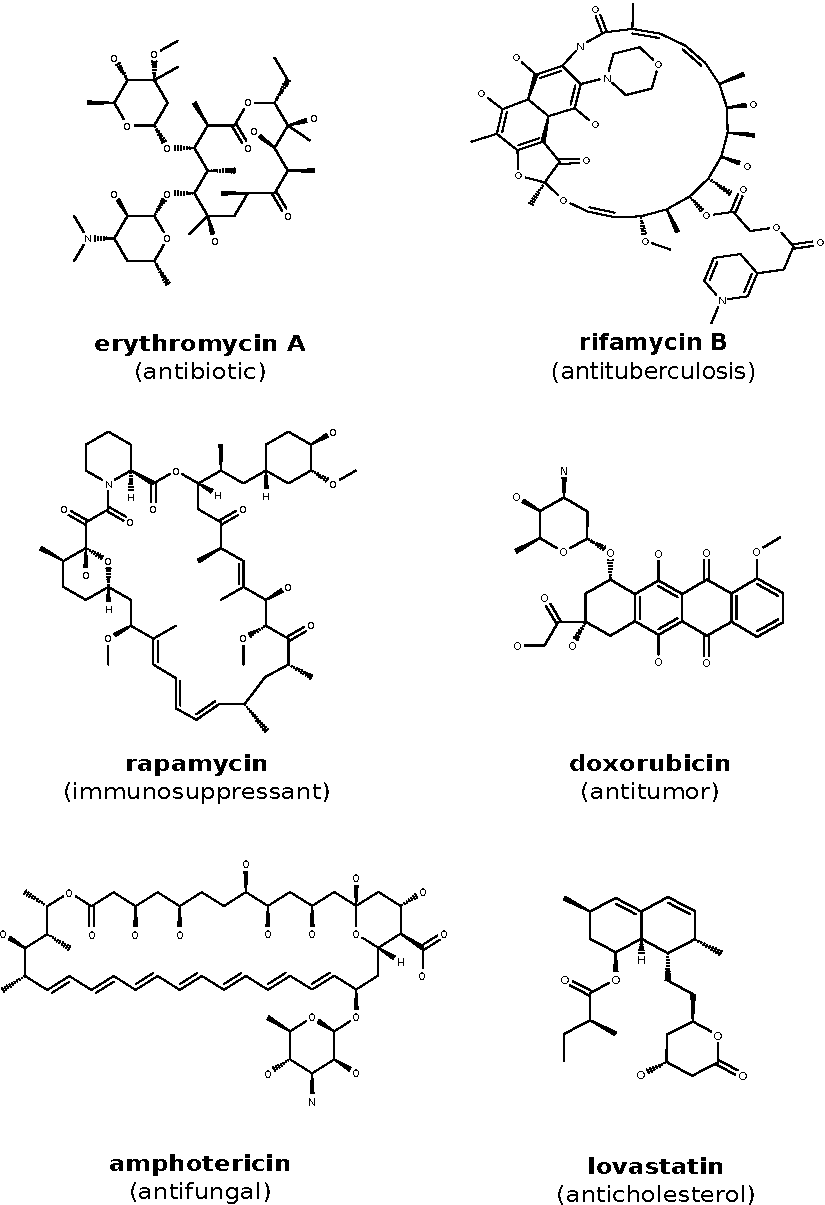
\includegraphics[width=0.9\textwidth, resolution=300, keepaspectratio=true]{graphics/polyketides.pdf}}
	\caption[Example polyketide compounds]{Example polyketide compounds (\url{http://www.drugbank.ca})}
	\label{fig:Polyketides}
	\end{figure}
	
	Polyketide and other natural product based drugs also have a huge market share, which drives pharmaceutical companies to continuously invest in research and manufacturing. Around 10,000 natural products had been identified by the year 1998 and many of these are being used as drugs. Between 1998-2004, 21 natural product based drugs were launched worldwide and around 19 were approved by the FDA between 2005-2010 \Parencite{Mishra2011, Mishra2011A}. Combined sales of erythromycin, FK506 and lovastatin exceeded \textdollar10 billion a year according to a news report in Science magazine published on 1 March, 2001 (\url{http://news.sciencemag.org/2001/03/bugs-making-drugs}).
	
	Polyketide research dates back to 1907 with the John Collie's work at London University on deducing the structure of orcinol \parencite{Collie1907}. However, the main impetus to the field came from Arthur Birch's work on 6-methyl-salicylic acid (6-MSA) produced by \textit{Penicilium patulum} in the 1950s. Arthur Birch explained the mechanism of 6-MSA production based on data from experiments feeding radioactively labelled acetate to the producing strain \parencite{Birch1955}. The labelled product was shown to have the same pattern as was to be expected from Birch's proposed mechanism. These observations of Collie and Birch later on came to be known as the Collie-Birch polyketide hypothesis, which explains that not only these complex natural products were a result of the condensation of simple acetate units, but also that they can be further transformed through enzymatic reactions to produce aromatic or cyclic compounds. 
		
	The detection of these compounds until the 1960s was based on deductive chemistry, where chemists break down the complex molecules into smaller recognizable moieties which were then intuitively assembled on paper \parencite{Powers2004}. Later on the advancement in spectrometric techniques such as mass spectrometry (MS) and nuclear magnetic resonance (NMR) completely transformed the research into easier and more accurate measurements. However, the detailed mechanistic view in the biosynthesis of these compounds and the genes/proteins involved was only possible after 1980s owing to the development of genetic manipulation methods. Genetic methods also enabled the scientific community to realize the potential for \textit{de novo} production of these compounds with altered functional groups. In the present era, with the new concept of synthetic biology, researchers are aiming to design synthetic machineries for the production of novel compounds that can be used for beneficial purposes. 
	
	\section{Polyketide synthases}	
	\label{sec:PKS}
	Polyketides are produced by multi enzyme complexes called polyketide synthases (PKSs). Not surprisingly PKS are equally as complex as polyketide compounds. It was only after the 1980s that researchers were able to characterize the genes and proteins involved in the PKS. The very first genes for a PKS were characterized by David Hopwood's group in 1984, for actinorhodin, an aromatic polyketide compound \parencite{Malpartida}. Later on Peter Leadlay and Leonard Katz independently identified the gene cluster responsible for the antibiotic erythromycin produced by \textit{Saccharopolyspora erythraea} \parencite{Cortes1990, Tuan1990}.
	
		\subsection{FAS and PKS analogous reaction mechanism}
		\label{sec:FAS}
		PKS share sequence and mechanistic similarity with the very well studied fatty acid synthases (FAS) \nomenclature{FAS}{Fatty acid synthase}. FAS synthesizes a relatively small group of saturated compounds as compared to the myriad of polyketides. Fatty acids are produced by a monotonous process of decarboxylative condensation of two ketone units followed by a series of reductive steps till a fully saturated molecule is achieved. The acyl transferase (AT) \nomenclature{AT}{acyltransferase} domain loads the starter (acetyl) and the extender units (malonyl) to the acyl carrier protein (ACP), \nomenclature{ACP}{Acyl carrier protein} which covalently tethers the ligand via a thioester bond to the long phosphopantetheine arm. The ACP transfers the starter or the extender units to the ketosynthase (KS) \nomenclature{KS}{Ketosynthase} for the decarboxylative condensation and also carries the newly synthesized product to be passed on to the other domains for further processing. Acting successively, keto reductase (KR) \nomenclature{KR}{Ketoreductase} reduces the \bet-keto group to a hydroxyl which is further reduced by a dehydratase (DH) \nomenclature{DH}{Dehydratase} to produce an alkene, this double bond is then reduced to a fully saturated chain by an enoyl reductrase (ER). \nomenclature{ER}{Enoyl reductase} The process of decarboxylative condensation and successive reductions continue till the fatty acid chain reaches to a required length, where upon it is then released by the thioesterase (TE) \nomenclature{TE}{Thioesterase} domain.
				
		Both PKS and FAS enzyme systems can be classified into type I, II, with an additional type III for PKS (more detail on PKS types in Section \ref{sec:PKStypes}). Type I FASs as found in mammals and fungi, are large multi domain complexes where the catalytic domains are covalently linked together in a long polypeptide chain. A single set of seven catalytic domains, as mentioned above, are utilized to produce a single molecule of fatty acid of the required length. Whereas, the type II FASs are free standing discrete mono functional catalytic units, used iteratively. Type II FASs are commonly found in bacteria, chloroplasts and mitochondria.
					
		In comparison to FAS machinery, PKS machinery is more complex and dynamic. PKSs vary the reductive steps on the \bet-keto acyl moiety after the condensation has happened, thus producing products with combinations of non modified \bet-keto groups, hydroxyl and enoyl groups. Several type I modular PKS were also found with modules lacking any condensation activity, for example the module 5 in the mmpA subunit of the mupirocin system. PKSs also have a choice of various starter and extender units \parencite{Khosla1999, Staunton2001}, in contrast to FASs which always start with acetyl and malonyl as the starter and extender unit respectively. Among many possible examples, of polyketide antibiotic pathways which utilize non conventional starter and extender units, as compared to the FAS, two examples are aureothin synthesis, which incorporates p-nitrobenzoate as the starter unit, and the erythromycin system which utilizes (2S)-methylmalonyl-CoA as the extender units.  PKS products are usually modified by various types of tailoring enzymes working \textit{in trans} for purposes such as cyclization, beta branching, epoxidation, pyran ring formation etc. Figure \ref{fig:FASandPKS} shows the generic reaction mechanism carried out by the FAS and PKS.
		
		\setlength\fboxsep{5pt}
		\setlength\fboxrule{1.5pt}
		\begin{sidewaysfigure} [htbp]
		\centering
		\fbox{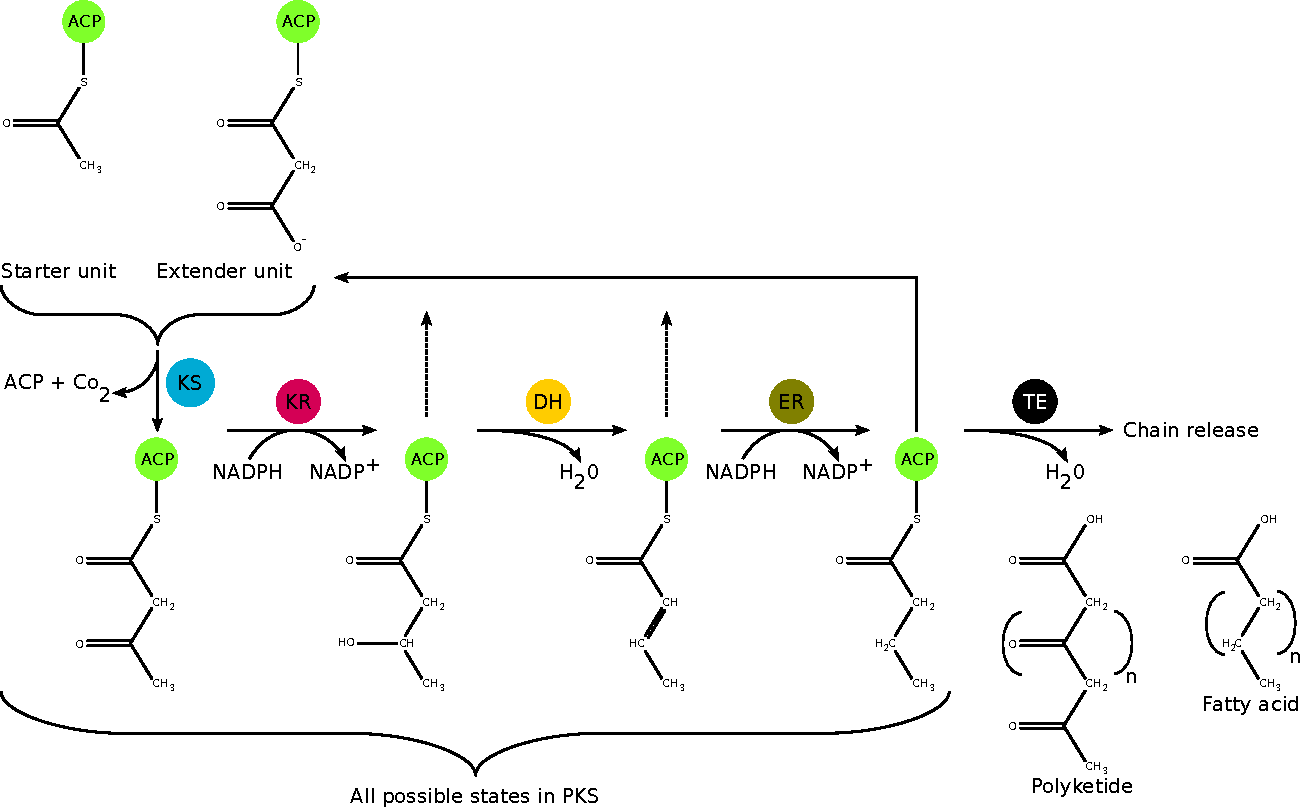
\includegraphics[width=0.9\textwidth, resolution=600, keepaspectratio=true]{graphics/FASandPKS.pdf}}
		\caption[Generic reaction mechanism for FAS and PKS]{Generic reaction mechanism for FAS and PKS. ACP: Acyl carrier protein; KS: Ketosynthase; KR: Ketoreductase; DH: Dehydrates; ER: Enoyl reductrase; TE: Tioesterase. In FAS the \bet-keto moiety in the elongated product is completely reduced to an acyl moiety as compared to the PKS in which it may or may not be partially or completely reduced thus producing keto, hyroxy and enoyl products. }
		\label{fig:FASandPKS}
		\end{sidewaysfigure}
		
		\subsection{FAS and PKS models}
		\label{sec:FASmodels}
		Over the years many research groups have proposed the likely domain organization and structural models for the FAS and PKS systems. The very first model proposed and widely accepted was the head to tail model in the 1970s which was later on overtaken by a newer head to head model for the FAS system and subsequently for the PKS as well. These simple models based on the domain organisation of the gene cluster and a few crosslinking experiments, helped researchers to understand FAS and PKS assembly until augmented by more accurate atomic resolution structures for full length FAS that were determined through X-ray crystallography. Although, researchers managed to successfully determine the structures for the FAS from various organisms we still lack a complete structure of a PKS. Some recent efforts have indeed produced structures of individual or binary domains from different PKS systems but a complete picture of an entire subunit or a module with all the catalytic domains is still missing.
			
			\subsubsection{Head to tail/head models for FAS}
			\label{sec:heatotail}
			Evidence in the 1970s and 1980s seemed to support the existence of a head to tail model for FAS structure and function (Figure \ref{fig:headandtail} A), but this was eventually superseded by a head to head model (Figure \ref{fig:headandtail} B)  In the 1970s many researchers observed that FAS mono functional units fail to catalyse chain elongation. FASs can be reversibly dissociated into functional units on exposure to low ionic strength buffers at cold temperature; the function restores in high ionic media at room temperature \parencite{Kumar1970,Smith1971}. The loss of elongation implied that for condensation to happen the active cite cysteine of the ketosynthase needs to be in close proximity of the phosphopantetheine arm of the ACP. Later on it was discovered that the active site cysteine of one subunit can be cross linked to the phosphopantetheine of the ACP on the other subunit by 1,3-dibromopropanone. This cross linking experiment was interpreted as meaning that the condensation required the interaction of KS and ACP from the opposite subunits \parencite{Stoops1983}. Another experiment on the FAS dimer with blocked thioesterase, showed two hanging fatty acids \parencite{Singh1984}. Additionally sequence analysis revealed that the ACP is located far away from the KS on the FAS cluster. Thus the above observations seemed to support the fully extended head to tail model where there were two reaction sites which were coordinated by the ACPs from the opposite subunit. 
		 	
		 	\setlength\fboxsep{5pt}
		 	\setlength\fboxrule{1.5pt}
		 	\begin{figure} [htbp]
		 	\centering
		 	\fbox{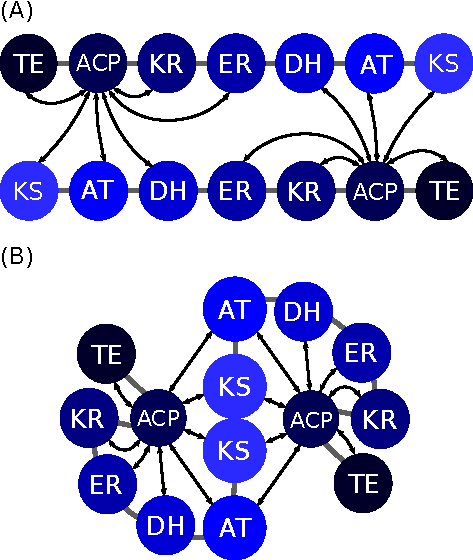
\includegraphics[width=0.8\textwidth, resolution=600, keepaspectratio=true]{graphics/headandtail1.pdf}}
		 	\caption[Head to tail/head models for FAS]{Head to tail/head models for FAS. (A) The fully extended head to tail model (B) The coiled head to head model. Figure adapted from \textcite{Smith2007}. }
		 	\label{fig:headandtail}
		 	\end{figure}
		 				
					
			Thus, the head to tail model gained a wide acceptance till it was challenged on the basis of the mutant complementation experiments. The complementation experiments showed that in the animal FAS the KS and ACPs can function together on either subunit \parencite{Witkowski1996}. Joshi and co-workers from the Smith group created several mutant knockouts in which different domains were inactivated. These mutant subunits were made to re-associate to create a mixed population of hetero and homo dimers. There findings revealed that homodimers formed by the KS, ACP, DH or TE mutant knockouts (at least one point mutation) and the hetero dimers formed by the ACP and TE mutant, ACP and DH mutant and DH and TE mutants were unable to carry out synthesis. However, heterodimers formed by KS and either DH, ACP, or TE mutants were able to carry out the synthesis at a reduced rate. These observations showed that the ACP and DH which are located far on the same subunit were able to interact which suggest that it was not necessary for the FAS to be in fully extended head to tail conformation. On the other hand a coiled state would explain the ability of the far placed ACP and DH to interact \parencite{Joshi1997,Joshi1998}.
		 	
		 	These observations lead to  questioning the interpretation of previously conducted crosslinking experiments, which had showed that 1,3-dibromopropanone can be used to cross link the active cite cysteine of ketosynthase to the phosphopantetheine arm of the ACP. The re-examination of the original cross linking experiment data revealed three bands, which would correspond to the double cross linked inter subunit species, single cross linked inter subunit species and single cross linked intra subunit species. If the interaction of the head to tail model, as in Figure \ref{fig:headandtail} (A), held true then there would have been only two bands for the single and double inter cross linked species. The presence of the third band indicates the possibility of the intra subunit KS - ACP interaction.
		 	
		 	To put the last nail in the coffin of the head to tail model, Joshi and co workers created an engineered mammalian FAS with only one functional subunit, all the domains from the other subunit were inactivated. This engineered FAS was able to catalyse all the biosynthetic steps in the fatty acid synthesis \parencite{Joshi2003}. These observations were enough to refute the requirement of the fully extended state of the head to tail model but would rather support the requirement of a scaffold which allows the domains on the two subunits to be accessible to their companion domain (Figure \ref{fig:headandtail} (B)).
		 	
 			This scaffold would support the newer head to head model in which the KS forms a dimer at the centre and the flanking domains coil around it, instead of KS being at the polar ends as in the head to tail model as  shown in Figure \ref{fig:headandtail} (A). This model also agrees with the KS in the FAS type II in which the KSs are known to exist as homo dimers and the active site is formed by the contribution of both the subunits \parencite{Moche1999, Olsen2001, Price2003}. Experiments carried out by Witkowski and co-worker showed that a truncated N terminal FAS (i.e. with incomplete KS) fails to dimerise. They also showed that the two KS subunits can be  cross linked via an engineered cysteine at the N terminal of the KS at a close proximity of 6 \AA{}. This crosslinking failed if one of the subunits lacks an engineered cysteine. They concluded their observation by performing mass spectrometry on the digested  cross linked product \parencite{Witkowski2004}.
 			
 			\subsubsection{Models for modular PKS}
 			\label{sec:CamPKS}
 			In the 1990s groups from the USA and UK lead by Khosla and Cane, and Staunton and Leadlay respectively, proposed the likely models for modular PKSs. The independent studies carried out by both the groups on the DEBS system using different methods agreed on the presence of two catalytic chambers for the condensation reaction in the modular PKSs. The studies also confirmed the dimeric nature of the PKSs similar to FASs. However, the proposed models by the two groups were strikingly different, details of which are discussed below. 
 			
 			The UK group in a series of experiments carried out limited proteolysis of the DEBS subunits using four proteases. The different sized fragments produced due to proteolysis were identified using N-terminal sequencing. They also determined the oligomeric state of the fragments using gel filtration and analytic ultracentrifugation. All the large fragments carrying the complete module were found to be homodimeric. The loading domain and the AT-ACP domains of the module 1 were found to be monomeric along with all the KR and ER domains in module 1,3,5 and 6 and module 4 respectively. On the basis of the cross linking experiment carried on the FAS (as mentioned in the previous section), the UK group used 1,3-dibromopropanone to cross link the 4'-phosphopantetheine moiety to the cysteine in the KS active site. The cross linking experiment confirmed an interaction between the KS and ACP from the opposite subunits \parencite{Aparicio1994, Staunton1996}.  
 			
 			These observations laid the basis for two models for the modular PKS, which were proposed to be parallel dimers. In the first model they proposed parallel dimers formed by the interaction of the KS and ACP at the interface and the other reductive domains protruding outwards from the axis, keeping all the domains at the reachable distance of the 4'-phosphopantetheine arm. In the second model (which alter came to be known as \textbf{Cambridge model}) the parallel dimers form a helical core utilizing KS, AT and ACP and the reductive domains again protrude away from the axis. Both the models showed the possibility of stacking multiple subunit on top of each other without affecting the functioning of the biosynthesis pathway. However, on the basis of the ultra-centrifugation results, that the protein dimer does not dissociate even at very low concentrations, the helical model was predicted and favoured to be more stable structure. These observations also proposed the inherent ability of the PKS to accommodate additional PKS which can be stacked with the rest of multi enzymes. Since the reductive domains protrude outside the dimeric core there is also a possibility of adding diversity to the reductive steps \parencite{Aparicio1994,Staunton1996}, as represented in Figure 3 A and B of \textcite{Staunton1996}.
 			
 			At the same time Khosla and Cane worked on finding the evidence for the domains participating in polyketide biosynthesis by generating several active site mutant PKSs. The experiments were performed \textit{in vitro} using DEBS 1 + TE, which consist of two modules along with an engineered TE domain. DEBS 1 + TE produces a cyclic triketide by utilizing propionyl-CoA and (2RS)-methylmalonly Co-A as starter and extender units respectively, and NADPH as the hydride donor. These experiments were carried out with the assumption that the modular PKS forms head to tail homodimers similar to the then prevalent idea for  mammalian FASs. In one study they produced three different active site DEBS 1 + TE mutants in which either the KS from module 1 or 2 or the ACP from module 2 was inactivated, refered to as KS1$ ^{0} $, KS2$ ^{0} $ and ACP2$ ^{0} $. These three parental mutant homodimers were utilized to produce three mutant heterodimers in which heterodimer a) consist of KS1$^{0}$ and KS2$^{0}$ , b) consist of KS2$^{0}$ and ACP2$^{0}$ and c) consist of KS1$^{0}$ and ACP2$^{0}$. The first two heterodimers were found to be active and were able to produce the triketide moiety however, the heterodimer c was unable to produce the triketide product. These observations gave substantial evidence that polyketide biosynthesis is based on the participation of two sets of active sites from opposite subunits and the cognate pair of KS and ACP can only be involved in the chain transfer \parencite{Kao1996}. These results were in contrast to FAS biosynthesis which allows chain elongation through either the KS-ACP pair from the opposite subunit or from the same. 
 			
 			In another study, following a similar mutant complementation strategy, Khosla and coworkers created an AT null mutant. This AT mutation was carried out in the module 2 and was paired with either the KS1$^{0}$ or KS2$^{0}$ mutants, thus generating two pairs of heterodimers. The aim of the experiment was to test whether the AT2 domain would be able to load the methylmalonyl extender unit to ACP2 from the same or the opposite subunit. If the loading of the extender unit is similar to the KS-ACP interaction from the opposite subunit then only the heterodimer carrying KS1$^{0}$ and AT2$^{0}$ should be active and not the heterodimer carrying KS2$^{0}$ and AT2$^{0}$. The complementation experiment showed that both the heterodimers were active and the AT domain were able to load the extender unit both inter and intra subunit. Kinetic studies showed no difference in the rate of extender unit loading  between the intra or inter subunit transfer \parencite{Gokhale1998}. 
 			
 			 	
		\subsection{Types of polyketide synthases}
		\label{sec:PKStypes}
		As mentioned in the previous sections, PKSs can be classified into three types, I, II and III where type I and II PKS are similar to FAS type I and II. Apart from the three canonical PKS types various PKS systems exist as hybrid with one or more other types. Hybrids also exists between one of the PKS types and a closely related non PKS system called non ribosomal peptide synthases (NRPS). The following sections describe the different PKS types in detail with relevant examples. 
			
			\subsubsection{Type I PKS}
			\label{sec:typeIPKS}
			Type I PKS are large single polypeptide multi domain protein complexes which can be further sub classified into modular and iterative types. As the name suggests, modular type I PKSs are composed of multiple modules where each module consists of all the necessary domains required for a single round of polyketide chain elongation and associated \bet-carbon processing. Whereas type I  iterative PKSs utilize a single set of covalently bound catalytic domains iteratively until the required length of the polyketide product with correct \bet-carbon processing is reached \parencite{Hertweck2009}. Type I modular PKSs are usually found in bacteria, for example the DEBS system in \textit{Saccharopolyspora erythraea} (Figure \ref{fig:DEBS}), whereas type I iterative PKSs are found in fungi for example the lovastatin system in \textit{Aspergillus terreus} (Figure \ref{fig:lov}). Type I modular PKSs can also be further classified as \textit{cis} and \textit{trans}-AT systems. \textit{Cis}-AT systems (e.g. DEBS) consist of a covalently fused AT domain within each module, which is responsible for loading the extender unit specific for the cognate module. Where as in \textit{trans}-AT systems (e.g. mupirocin) the AT domain is not covalently fused within each module but it exists as a separate discrete domain. \textit{Trans}-ATs are responsible for loading the starter unit at the beginning of the pathway as well as the extender units at each module throughout the pathway. 
			
			In type I modular PKSs since each module is responsible for a single step of chain extension and subsequent \bet-carbon processing, it is possible to deduce the product being produced just by studying the sequence in which the modules are arranged in the biosynthetic cluster. This collinearity rule has enabled the development of various computational methods to predict the probable metabolite being produced directly from the DNA or protein sequence. Section \ref{sec:BioinfoPKS} gives a more detailed account of the computational methods developed till now to predict the polyketide as well as other secondary metabolites from their biosynthetic gene/protein cluster. Although this collinearity rule in type I modular PKSs is effective in predicting metabolite production straight from the sequence, it does not hold true in \textit{trans} AT systems and in systems where a certain module is used iteratively or skipped altogether. 
			
			\setlength\fboxsep{5pt}
			\setlength\fboxrule{1.5pt}
			\begin{sidewaysfigure} [htbp]
			\centering
			\fbox{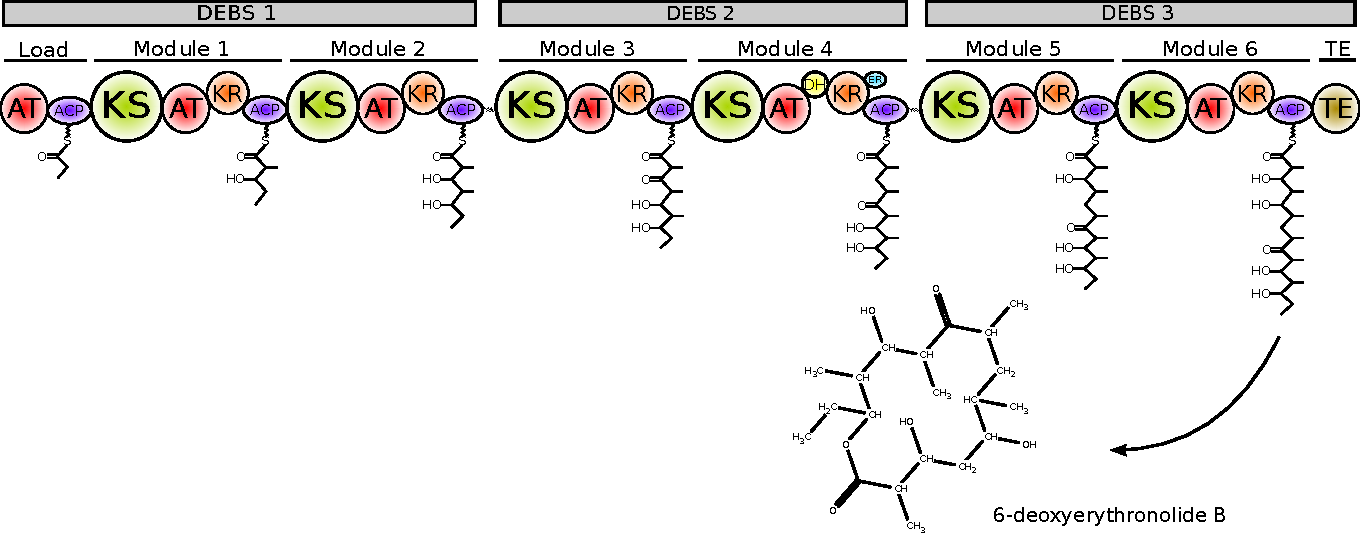
\includegraphics[width=\textwidth, resolution=600, keepaspectratio=true]{graphics/debs.pdf}}
			\caption[Type I polyketide synthases (modular and cis AT) from 6-deoxyerythronolide B synthase
			(DEBS) system.]{Type I polyketide synthases (modular and cis AT) from 6-deoxyerythronolide B synthase
			(DEBS) system.  The DEBS system consist of 28 domains spread across 3 polypeptides (DEBS 1, 2 and 3) of ~350 kDa each, with each polypeptide containing two modules. Abbreviatiosn: KS, ketosynthase; AT, acyltransferase; ACP, acyl carrier protein; KR, ketoreductase; KR 0, inactive ketoreductase; DH,
			dehydratase; ER, enoylreductase. Figure adapted from \parencite{Khosla2007}
			}
			\label{fig:DEBS}
			\end{sidewaysfigure}
			
			For many years DEBS served as the model system for studying type I modular PKS. DEBS is responsible for the production of 6-deoxyerythronolide B which acts as a precursor in the production of the  antibiotic erythromycin. The DEBS system consists of 28 domains spread across 3 polypeptides (DEBS 1, 2 and 3) of ~350 kDa each, with each polypeptide containing two modules (Figure \ref{fig:DEBS}). DEBS 1 contains an extra module which consists of an AT and ACP domain prior to the condensing module 1. This extra module is responsible for priming the KS in module 1 with a propionate unit. DEBS 3 contains a TE domain after module 6, for polyketide release. Each module in the DEBS system is responsible for a single round of Claisen condensation utilizing methyl malonate as the extender unit. Every module in the DEBS system also performs \bet-keto reduction of the condensed product and only module 4 further reduces the \bet-carbon with a dehydratase and an enoyl reductase (Figure \ref{fig:DEBS}) \parencite{Khosla2007}. Due to the modular nature of the DEBS system and ease of cloning the DEBS genes into an appropriate host like \textit{S. coelicolor} and \textit{E. coli}, many research groups exploited the DEBS machinery to understand and elaborate the re-engineering capability of modular type I PKSs. Section \ref{sec: reengineer} explains an example of successes and challenges in re-engineering PKSs.  
			
			\setlength\fboxsep{5pt}
			\setlength\fboxrule{1.5pt}
			\begin{figure} [htbp]
			\centering
			\fbox{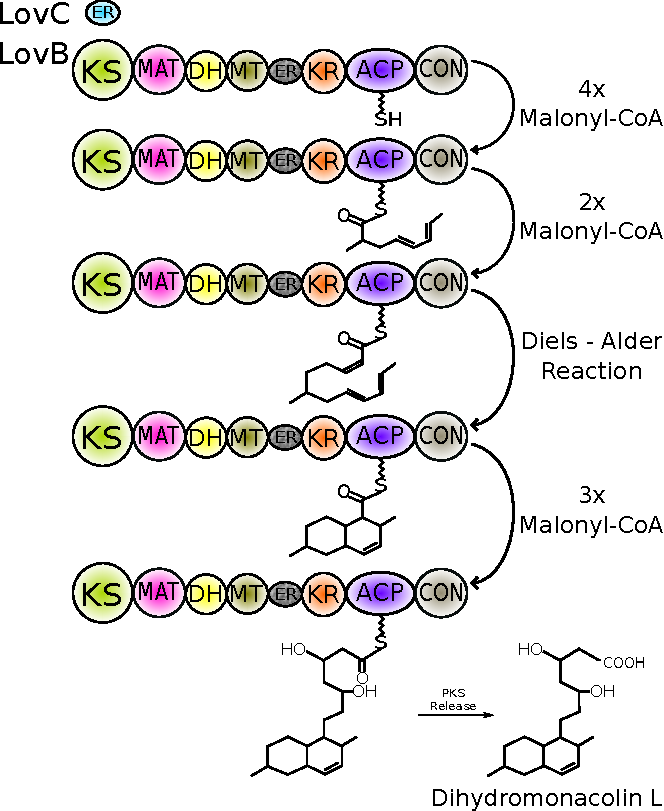
\includegraphics[width=0.7\textwidth, resolution=600, keepaspectratio=true]{graphics/lov.pdf}}
			\caption[A Type I polyketide synthase (iterative), the lovastatin system.]{ A Type I polyketide synthase (iterative), the lovastatin system. The figure here only shows the PKS LovB out of the two PKSs LovB and LovF utilized in the production of lovastatin. LovB is responsible for the production of dihydromonacolin L moiety which is produced by the iterative condensation of 9 malonyl-CoA extender unit. LovB carries a non functioning ER domain for which the function is substituted by LovC. The other domains in LovB consist of a ketosynthase, a malonyl transferase (MAT), a methyl transferase (MT), a dehydratases (DH), an enoyl reductases (ER), a ketoreductases (KR), an acyl carrier protein (ACP) and a condensation domain (CON).
			}
			\label{fig:lov}
			\end{figure}
			
			Another popular and well studied example is the type I iterative PKS that produces lovastatin, which is produced by the fungi \textit{Aspergillus terreus}. Lovastatin is a cholesterol lowering agent which acts as a precursor for the popular drug simvastatin. The lovastatin biosynthesis pathway consist of two PKSs LovB and LovF. LovB, which is responsible for the nonaketide moiety dihydromonacolin L, consists of a ketosynthase, a malonyl transferase (MAT), a methyl transferase (MT), a dehydratases (DH), an enoyl reductases (ER), a ketoreductases (KR), an acyl carrier protein (ACP) and a condensation domain (CON) (Figure \ref{fig:lov}). The ER domain in LovB is non functional therefore LovB utilizes a free standing ER LovC. LovB utilizes 9 malonyl-CoA extender units, a methyl donated from a S-adenosyl-L-methionine (SAM) molecule and an NADPH to produce dihydromonacolin L. LovF consists of all the above mentioned domains but it has a functional ER. LovF catalyses the formation of the 2-methylbutyrate moiety by the condensation of two acetyl units. Other enzymes encoded within the same gene cluster includes LovA and LovD. LovA encodes a cytochrome P450 oxygenase which oxidises the dihydormonacolin L produced by the LovB, which is covalently joined to the 2-methylbutyrate moiety by the trans esterase activity of the LovD. Figure \ref{fig:lov} shows the production of dihydromonacolin L by LovB and LovC in the lovastatin biosynthesis pathway, and includes  the proposed stage of a Diels-Alder reaction for ring formation in the growing polyketide \parencite{Kennedy1999,Ma2007, Campbell2010, Ames2012}. 
			
			Apart from the minimal PKS domains and one or more required \bet-keto processing domains, several type I PKS gene clusters contain a number of tailoring enzymes which perform further different functions at different stages of polyketide synthases. These tailoring enzymes may act on the ACP bound polyketide intermediate or on the released product post production. One such tailoring enzyme is 3-hydroxy-3-methyl glutryl-CoA synthase cassette (HCS) which is responsible for the \bet-branching in many type I PKS systems for example mupirocin, thiomarinol and kalimantacin \parencite{Haines2013}. The HCS cassette adds a methyl branch at the \bet-position of the growing polyketide chain by the coordinated action of five enzymes which include an ACP, an HMG-CoA synthase, two enzymes from the crotonase family and a decarboxylase. This \bet-methylation step is considered to be rate limiting and more complex as compared to the methylation of an $\alpha$ carbon by a methyl transferase. At the onset of \bet-methylation an ACP delivers a polyketide intermediate to the HMG-CoA domain in the HCS cassette. This delivery requires the ACP and the HMG-CoA from the HCS to interact and recognize each other at the appropriate stage of polyketide synthesis. At the time of starting my thesis, it was not very well understood what enables the HCS cassette to recognize the correct ACP for the \bet-branching. One of the projects in the present study was to explore the specificity mechanism of ACP-HCS interaction in the mupriocin pathway, which is described in Chapter \ref{cha:ACP-HCS}.
			
			Another recently discovered tailoring enzyme of interest is halogenase. In the curacin system this halogenase domain works in conjunction with the HCS proteins and is responsible for the addition of a chloride on the $\gamma$ carbon in the growing polyketide chain. In a study published by \textcite{Busche2012}, they found the recognition specificity between this halogenase domain and the ACP. Advances in PKS research are slowly unfolding the details of several different pathways, with a diversity of enzymes functioning in conjunction core PKS function. It is becoming increasingly interesting to understand structure function relationship of these auxiliary enzymes and to exploit them for synthetic biology purposes.
			
			\subsubsection{Type II PKS}
			\label{sec: typeIIPKS}
			Type II polyketide synthases produce aromatic compounds (polyphenols) in Gram-positive bacteria of the class actinomycetes, found in soil and marine environments. Some of the famous examples of type II polyketides are tetracyclines, which is a class of broad spectrum antibiotics, and doxorubicin, which is an anti cancer agent. In contrast to the type I PKSs, where all the catalytic domains are covalently bonded in a single polypeptide chain, the domains forming the type II PKS are encoded on separate genes. However, the genes encoding the type II domains are usually found to be clustered together. Type II PKSs utilize an acyl starter unit and a malonyl extender unit for Claisen condensation, using a single set of mono functional enzymes iteratively. A minimal set of a type II PKS domains comprises of two KSs, a KS$_{\alpha}$ and a KS$_{\beta}$ domain, and an ACP domain. Other catalytic domains such as ketoreductases and aromatases amongst others perform \bet-keto processing. It is much more difficult to study type II PKS as compared to type I PKS due to the very short span of stability of the intermediates produced. With type II PKS it is also not possible to predict the metabolites produced straight from the sequence of the biosynthetic domains involved, which is much simpler in type I modular PKS \parencite{Hertweck2007}. 

			\setlength\fboxsep{5pt}
			\setlength\fboxrule{1.5pt}
			\begin{sidewaysfigure} []
			\centering
			\fbox{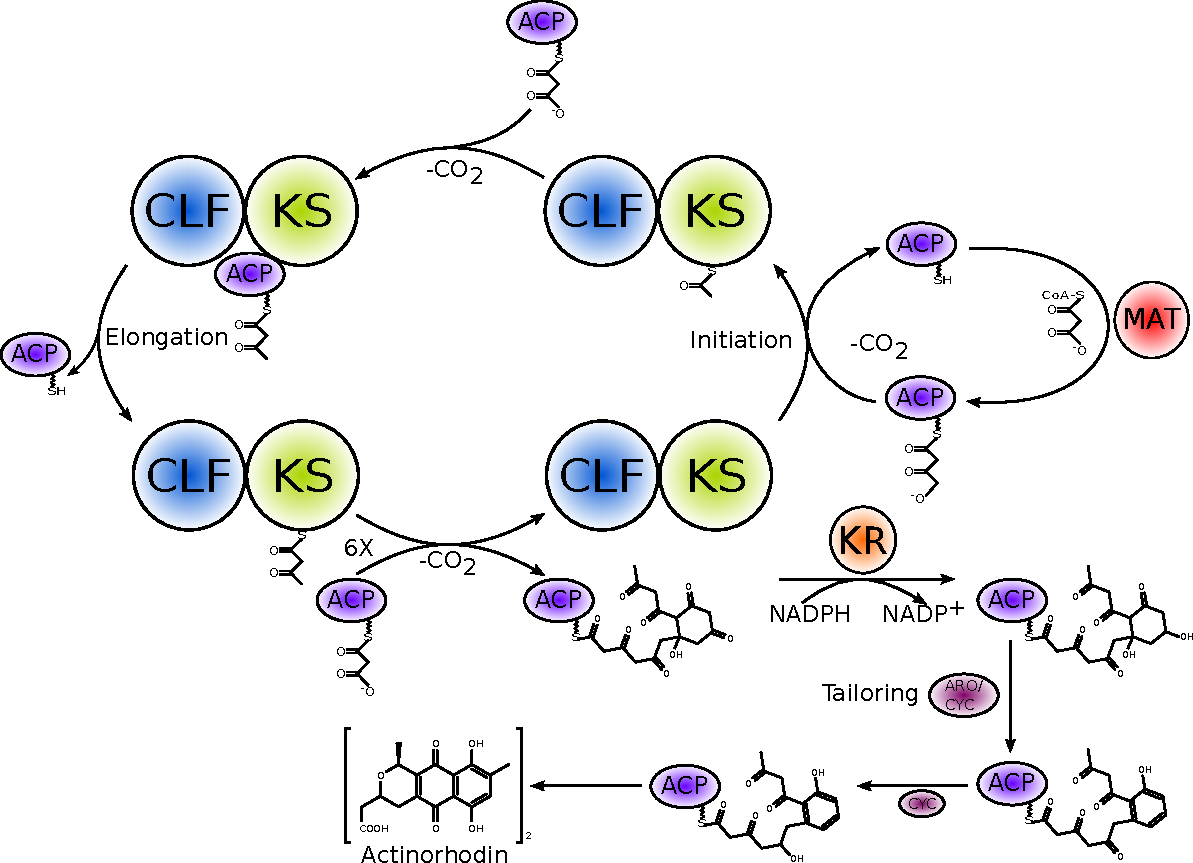
\includegraphics[width=0.7\textwidth, resolution=600, keepaspectratio=true]{graphics/actpathway.pdf}}
			\caption[Type II polyketide synthases from actinorhodin biosynthesis pathway]{Type II polyketide synthases from actinorhodin biosynthesis pathway. The chain length factor (CLF) and ketosynthase (KS) form a heterodimer. The malonyl-CoA:ACP transacylase (MAT) primes the ACP with the malonate unit. The biosynthesis begins with the decarboxylation of a malonyl unit on to the KS followed by the Claisen condensation with an activated malonyl unit. Overall 7 rounds of Claisen condensation takes place to reach the required length. Upon release the product undergoes post synthesis processing with aromatase and cyclase enzymes to produce actinorhodin molecule. Figure adapted from \parencite{Das2009}.}
			\label{fig:ACT}
			\end{sidewaysfigure}
						
			The KS$_{\alpha}$ and KS$_{\beta}$ domains form heterodimers, where KS$_{\alpha}$ is responsible for Claisen condensation and KS$_{\beta}$ keeps a check on the synthesized chain length, also known as \textquoteleft chain length factor\textquoteright (CLF). \nomenclature{CLF}{Chain length factor} KS$_{\beta}$ lacks a catalytic cysteine and therefore it can not perform Claisen condensation but upon mutating the position where a catalytic cysteine would be expected to a glutamine (KS$_Q $) it is capable of decarboxylating the malonyl unit into an acetate \parencite{Keatinge-Clay2004a}. This KS$_Q$ functionality is similar to the KS$_Q$s found in the modular type I PKS where they are utilized to convert a malonyl unit into an acetate starter unit \parencite{Bisang1999}. Swapping CLF from different type II PKS can result in the production of metabolites of different chain lengths.
			
			It is still not very well understood what catalyses the loading of a malonyl unit to the ACP of a type II PKS. Two alternative hypothesis were proposed both with similar possibility and experimental evidence. One hypothesis favours the self malonylation of the ACP, which was experimentally verified \textit{in vitro} in a purified sample of type II PKS \parencite{Arthur2005}. The other hypothesis argues a potential involvement of a malonyl-CoA:ACP transacylase  (MAT) but most of the type II PKS cluster lacks an MAT therefore it was hypothesized that this MAT is borrowed from a FAS in the cell \parencite{Dreier1999,Keatinge-Clay2003}. Type II PKS are also found to utilize domains such as KR, DH and ER from the host FAS \parencite{Tang2006a}. 
						
			Figure \ref{fig:ACT} summarizes the biosynthetic pathway of the type II antibiotic actinorhodin produced by \textit{Streptomyces coelicolor} as an example of a type II PKS. Actinorhodin biosynthesis initiates by the priming of the malonate unit onto an ACP by the malonyl-CoA transacylase. The malonyl-CoA unit is decarboxylated and transferred to the cysteine thiol of the KS$_{\alpha}$ which acts as the starter unit. This step is followed by seven iterative Claisen condensation cycles. At the end of the condensation cycles the intermediate product undergoes keto reduction and successive aromatization and cyclization to produce the polycyclic end product actinorhodin. Actinorhodin biosynthesis is carried out purely by  a minimal set of type II  PKS followed by downstream processing with tailoring enzymes however, other secondary metabolites like R1128 and doxurubicin require an initiation module to produce a diketide starter unit prior to the minimal type II PKS activity. This initiation module consists of a KS homodimer and an ACP, the absence of the CLF suggests the non requirement of chain length control in this module. Further details, including a cartoon representation of an initiation module, are given elsewhere \parencite{Das2009}.
			
			\subsubsection{Type III PKS}
			\label{sec: typeIIIPKS}

			\setlength\fboxsep{5pt}
			\setlength\fboxrule{1.5pt}
			\begin{sidewaysfigure} []
			\centering
			\fbox{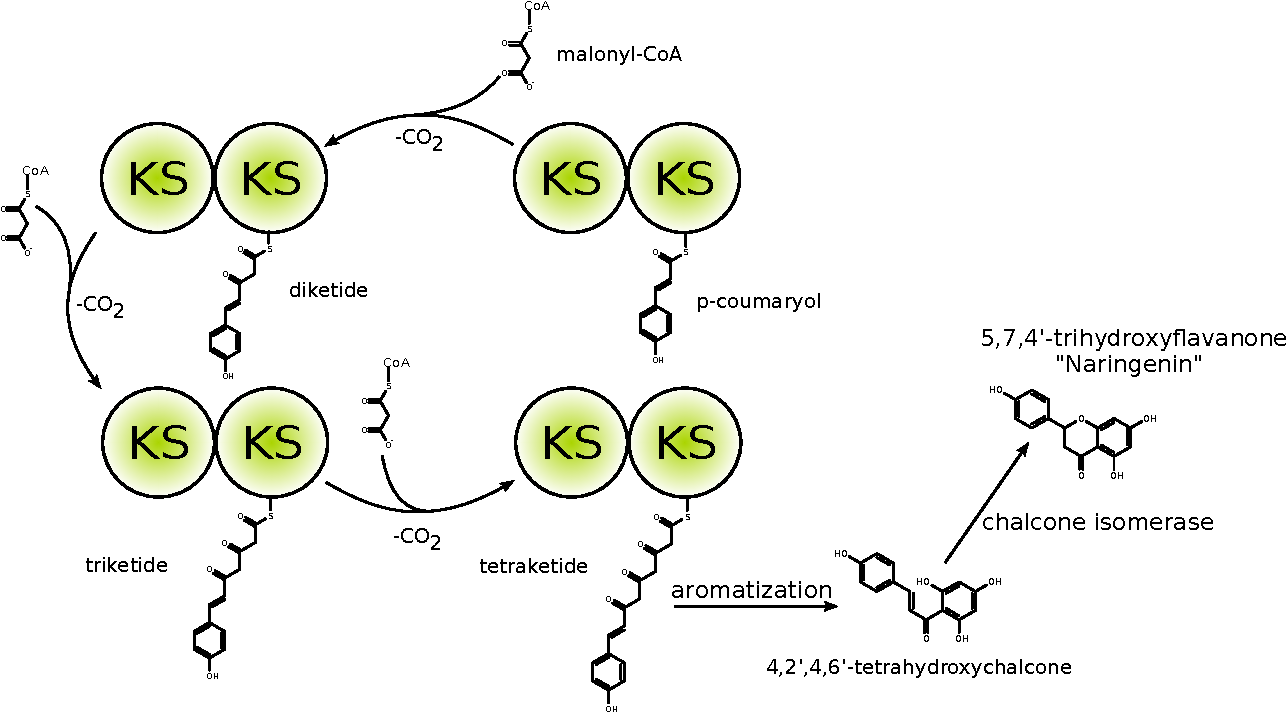
\includegraphics[width=\textwidth, resolution=600, keepaspectratio=true]{graphics/chs.pdf}}
			\caption[Proposed reaction mechanism of Type III polyketide synthases/Chalcone synthase]{Proposed reaction mechanism of Type III polyketide synthases/Chalcone synthase. The growing metabolite is shown attached to one of the KS of the homodimer. The p-coumarocyl-CoA starter unit is condensed iteratively with three acetate units derived from malonyl-CoA, followed by aromatization and chalcone isomerization to produce Naringenin. Figure adapted from \parencite{Ferrer1999}.}
			\label{fig:CHS}
			\end{sidewaysfigure}
						
			Type III PKS commonly found in plants, but with recent discoveries in bacterial systems as well, belong to the superfamily of chalcone synthases (CHS) \nomenclature{CHS}{Chalcone synthases} / stilbene synthases (STS) \nomenclature{STS}{Stilbene synthases}. CHS is the first step in the plant flavanoid biosynthesis and is responsible for a variety of plant metabolites, with functions including defence, pigmentation and fertility.  CHSs utilizes a single homodimeric ketosynthase iteratively, catalyses Claisen condensation of a p-coumaroyl-CoA, as a starter unit, to the three acetate units derived from malonyl-CoA. The same catalytic centre is also further utilized for successive aromatization and cyclization to produce chalcone. Figure \ref{fig:CHS} explains the chalcone biosynthetic pathway proposed by \textcite{Ferrer1999}. PKS type III represents a divergent class of this CHS functionality with the diversity in the choice of starter units, extender units, number of chain extensions and subsequent cyclization. There were differences found in the bacterial and plant type III PKSs, for example bacterial type III PKS can utilize an acyl-ACP starter unit by involving an ACP from an FAS, whereas plants use acyl-CoA as the starter unit. Based on structural analysis of the type III PKS ketosynthase \textcite{Qiu2001a} have suggested the emergence of these enzymes from the fatty acid KAS III. FAS KAS III are responsible for the initiation of type II FAS biosynthesis. The type III PKS utilizes CoA thioesters instead of a phosphopantetheinylated ACP to tether the growing polyketide product \parencite{Austin2003}. 
			
		\subsection{PKS domains}
			\subsubsection{Acyl carrier protein (ACP)}
			\label{sec: ACP}
			Acyl carrier proteins (ACP) belong to a class of carrier proteins which are involved in channelling the substrates via a phosphopantetheine prosthetic group. These carrier proteins are known to be involved in fatty acid synthesis (FAS), polyketide synthesis (PKS) and non-ribosomal peptide synthesis (NRPS) \nomenclature{NRPS}{Non Ribosomal Peptide Synthase}. The carrier proteins involved in FAS and PKSs are called ACPs, but peptidyl carrier proteins (PCP) \nomenclature{PCP}{Peptidyl Carrier Proteins} in NRPSs. In FAS the same ACP domain is utilized iteratively to pass the substrate to the different domains of the module multiple times whereas in PKSs, especially in type I modular PKS, each module has its cognate ACP to perform the substrate channelling for that module. Although the carrier proteins share a wide range of sequence identity among various organisms, they still share a common structural fold. A sequence identity of \textgreater80\% is reported between ACPs from \textit{E. coli} and \textit{V. harveyi}, whereas 21\%-27\% sequence identity between \textit{E. coli} and rat ACPs \parencite{Byers2007}.  A common carrier protein fold consists of a 4 helical bundle which ranges from 70 to 100 amino acids long. Among the three major $\alpha$ helices, helix I runs antiparallel to helix II and IV with a small helix III which runs almost perpendicular to the axis of the three major helices. Inspite of their small structure carrier proteins are found to exhibit great degree of plasticity in their backbone movement. FAS ACPs are found to sequester the growing fatty acid chain within the hydrophobic pocket in the centre of ACP \parencite{Chan2008}. On the other hand NRPS PCPs have been shown to be involved in backbone rearrangement and helical movement during substrate chanelling \parencite{Koglin2006}. However, no such intrinsic conformational motion has yet been reported in PKS ACPs, which is discussed in more detail in Chapter \ref{cha:chap5}. These carrier proteins are translated as inactive apo proteins that are activated by addition of the 4\textquoteright-phosphopantetheine moiety of a coenzyme A, through the action of 4\textquoteright-phosphopanthetheine transferase \parencite{Mootz2001}. This 4\textquoteright-phosphopantetheine moiety is attached to a conserved serine at the end of the helix II via a phosphodiester bond (see Figure \ref{fig:acp}). Carrier proteins have also been found to be abundant in various organisms, with 80 reported in \textit{Streptomyces avermitillis}.
					
			In a typical PKS pathway an ACP has to interact with a large number of proteins which include 
			\begin{inparaenum}[\itshape 1\upshape)]
			\item an AT domain, either \textit{cis} or \textit{trans} 
			\item an upstream KS domain 
			\item a downstream KS domain 
			\item other catalytic domains for example KR, DH, ER, and
			\item several other tailoring enzymes. 
			\end{inparaenum}
			Until recently it was not known how the relatively small structure of the carrier proteins interact with such a diverse set of interacting partners. There were several unanswered questions such as, how much of the carrier protein\textquoteright s surface interacts with the partner protein? Does each interaction occur at a different face of the protein? What drives the phosphopantetheine arm to the different catalytic domains? Some of these questions have been answered lately however, there is still a lot to be discovered. 

			
			\setlength\fboxsep{5pt}
			\setlength\fboxrule{1.5pt}
			\begin{figure} []
			\centering
			\fbox{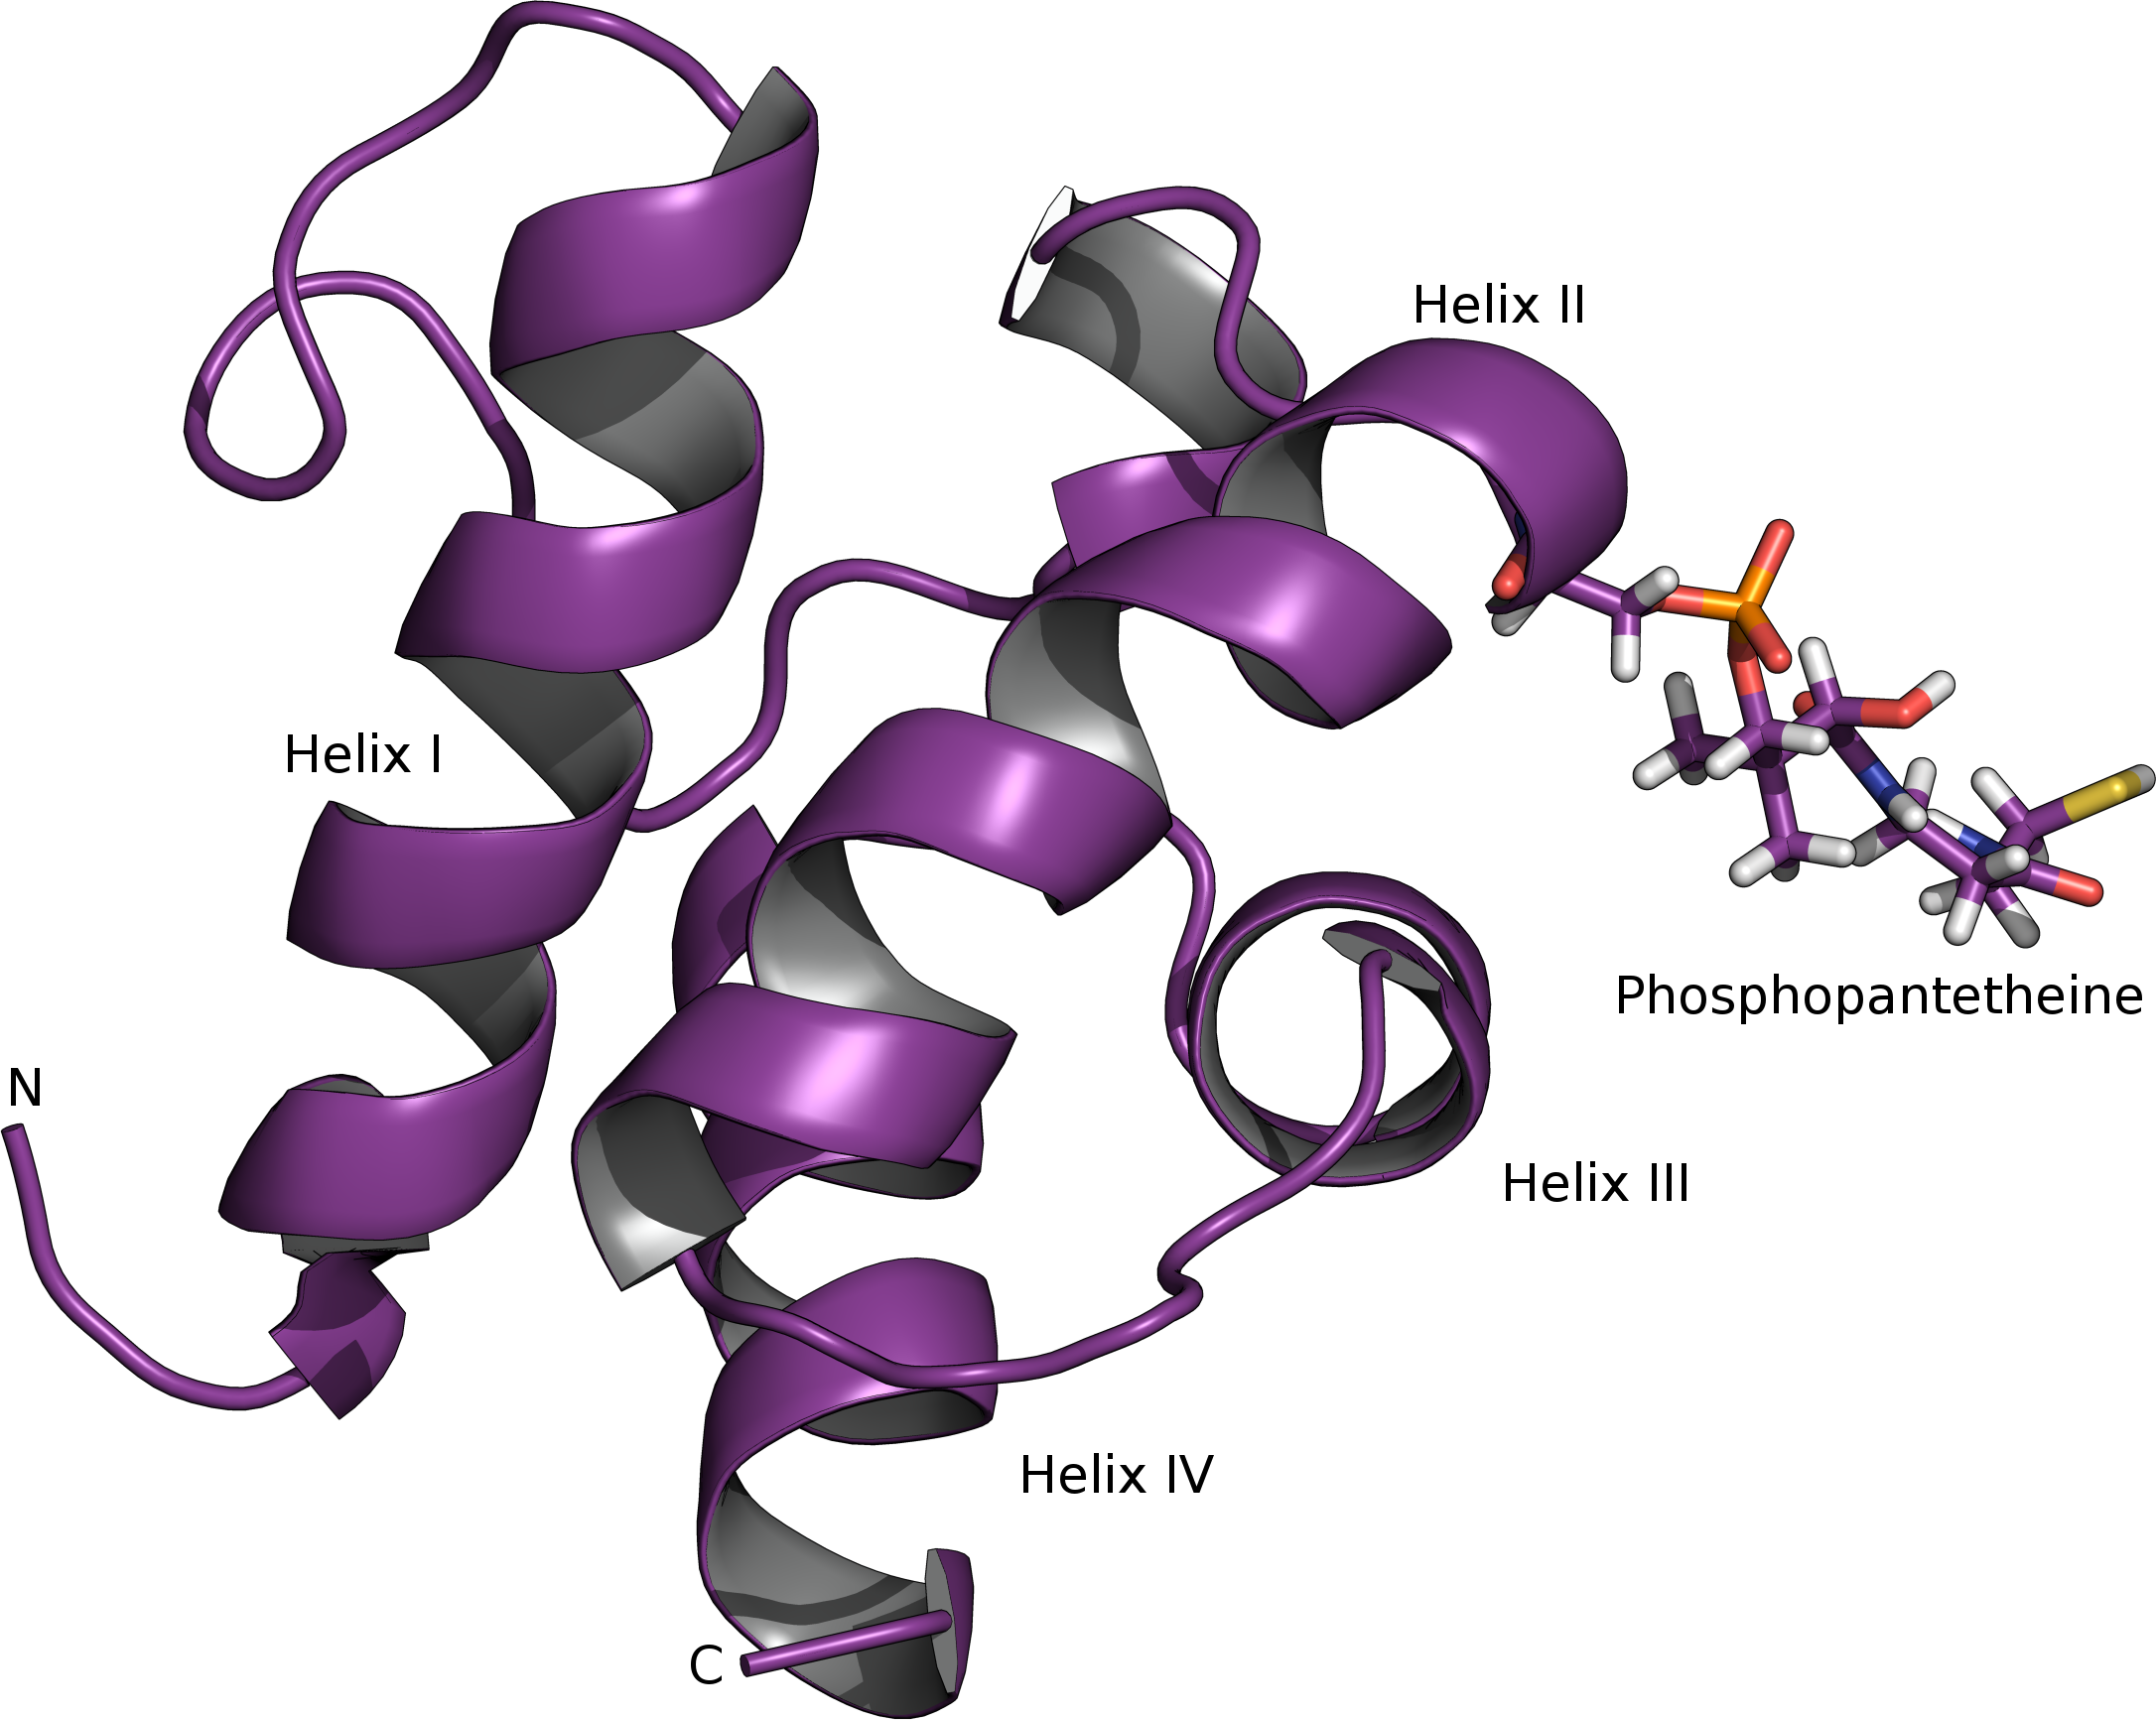
\includegraphics[width=\textwidth, resolution=600, keepaspectratio=true]{graphics/acp.png}}
			\caption[Cartoon representation of an acyl carrier protein from mupirocin pathway]{Cartoon representation of an acyl carrier protein (ACP-A3a) from the mupirocin biosynthesis pathway (PDB ID 2L22). A phosphopantetheine arm is modelled attached to the catalytic serine, represented as sticks \parencite{Haines2013}. }
			\label{fig:acp}
			\end{figure}
			
			
			In a study of FAS ACPs by \textcite{Zhang2003} helix II was shown to interact with various interacting partners as the \textquotedblleft recognition helix\textquotedblright. Helix II being conserved and negatively charged interacts with the positively charged channels of various ACP dependent proteins \parencite{Zhang2001}. However, studies by Khosla's group of PKSs have shown by structural modelling and mutagenesis work that loop I and helix I are the interacting interface for the chain elongation and translocation steps respectively. In another study on curacin biosynthesis helix III on the ACP was found to be interacting with and the halogenase enzyme \parencite{Busche2012}. In the present work as well, helix III is shown to be one of the anchors that interacts with  MupH, as described in Chapter \ref{cha:ACP-HCS}. Thus, it can be said that helix II, which was considered to be the \textquotedblleft recognition helix\textquotedblright, is not the only surface with which ACPs interact with other proteins. Further exploration may lead to finding some other novel features not yet discovered.
			
			Till now there are only 6 entries in the PDB representing 4 different structures solved for the ACPs from PKS systems, 2 for each \textit{cis} and \textit{trans} AT systems. The first set of structures for the \textit{cis} AT PKS were published in 2007 from module 2 of the DEBS system (PDB ID 2JU1, 2JU2) \parencite{Alekseyev2007}, followed by the structure of ACP1 from the CurA module of curacin system (PDB ID 2LIU, 2LIQ) in 2012 \parencite{Busche2012}. Structures from the trans AT systems came out very recently in 2013 for the didomain ACP in the MmpA subunit of the mupriocin system which are involved in \bet-branching mechanism (PDB ID 2L22) \parencite{Haines2013} followed by the solution structure of ACP 5 from the virginiamycin cluster (PDB ID 4CA3) in early 2014 \parencite{Davison2014}.
			
			\subsubsection{Acyl transferases (AT)}
			\label{sec:AT}
			In PKS and FAS systems acyl transferase domains are responsible for loading the starter and extender units onto the ACPs. In the type I modular PKS systems the AT domains can either be covalently bound in the same polypeptide chain, which are called \textit{cis} AT e.g. as in erythromycin synthesis, or can exist in \textit{trans} as discrete domains e.g as in mupirocin synthesis. In FAS systems, the acetyl starter and malonyl extender moiety are transferred on to the same AT domain, at different times, via acetyl/malonyl transferase from an acetyl-CoA/malonyl-CoA molecule. Thus, an FAS AT domain has dual specificity for the starter and extender units and there is a competition between the two substrates for the AT active site. This phenomenon also holds in many \textit{trans} AT PKS systems, for example mupirocin, where a single set of AT domains is responsible for loading both the starter and the extender units. On the other hand, \textit{cis} AT PKS systems have a separate module for loading the starter unit and the AT domain that is covalently bound to a particular module allows loading its cognate extender unit. Thus in principle AT domains can have specificity towards their own extender units allowing different extender units to be utilized at each elongation step \parencite{Khosla1999}. 
			
			The AT domain catalyses the starter and extender unit's transfer from a  CoA on to the phosphopantetheine of an ACP. This transfer is achieved by a ping-pong bi-bi reaction mechanism utilizing a conserved SER-HIS diad (e.g. S642 and H745 in DEBS AT5). The malonyl or methyl malonyl moiety was found to interact with the conserved active site ARG (e.g. R667 in DEBS AT5) at the beginning of the reaction \parencite{Tang2006}. The catalytic SER resides in  a highly conserved motif, GHSXG, and is responsible for the nucleophilic attack on the carbonyl of the acyl moiety offered by the CoA. This nucleophilic attack leads to the formation of a SER-acyl tetrahedral geometry, which is hypothesized to be stabilized by an oxyanion hole formed by the backbone amides (e.g. Q9 and V98 in S. coelicolor MAT structure), and to the release of CoA \parencite{Keatinge-Clay2003}. HIS in the diad helps to enhance the nucleophilicity of the SER. In the second step of the reaction the thiol of the incoming phosphopantetheine initiates a nucliophilic attack on the SER bound acyl carbonyl forming SER-acyl-ACP tetrahedral intermediate which is released by the protonation of the active site SER by the active site HIS (Figure \ref{fig:ATreact}) \parencite{Tsai2009, Dunn2013}. 
			
			Figure \ref{fig:AT} shows the cartoon structure of an AT domain from the module 5 of the DEBS system and the proposed reaction mechanism is shown in Figure \ref{fig:ATreact}. AT domains follow  an $\alpha$/$\beta$-hydrolase fold as the core catalytic domain of approx 240 residues attached to a smaller ferredoxin like  domain of approx 60 residues. The N-terminus of the AT domains in the \textit{cis}-AT systems are found to contribute to the KS-AT linker (approx 140 residues) which is termed equivalent to the docking domain in the \textit{trans}-AT systems \parencite{Tang2006, Gay2014}. However, the docking domain in the \textit{trans}-AT systems does not carry any portion of the AT domain but is formed by the linker sequence in between the KS and the subsequence domain \parencite{Gay2014}. This linker region in the \textit{cis} system (DEBS) is found to be important for the interaction of the ACP during chain transfer and elongation \parencite{Kapur2010, Kapur2012}. Although the crystal structure of a docking domain attached to the KS in the trans AT system was recently published the role of the docking domains are still not understood \parencite{Gay2014}. 
			
			\setlength\fboxsep{5pt}
			\setlength\fboxrule{1.5pt}
			\begin{sidewaysfigure} []
			\centering
			\fbox{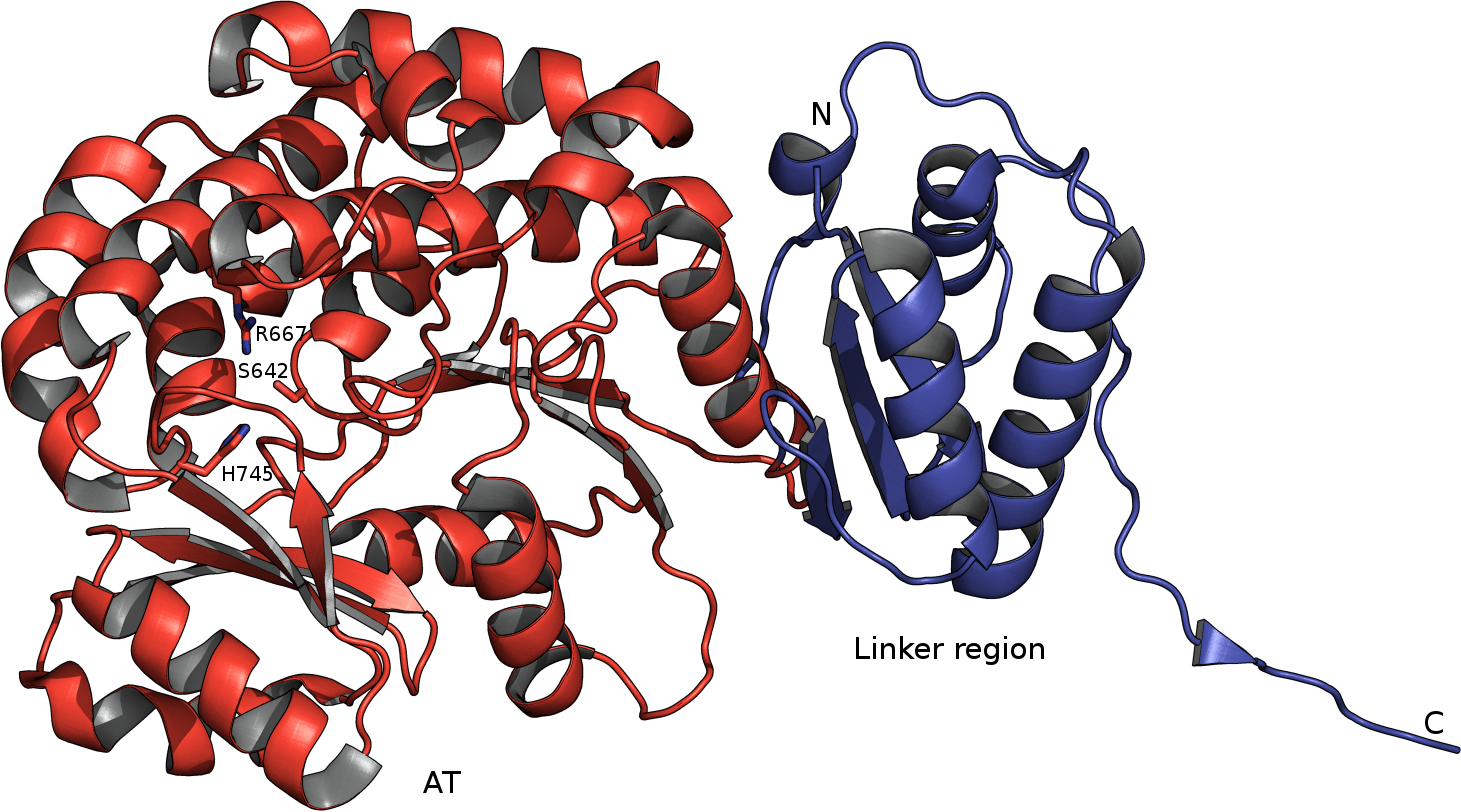
\includegraphics[width=\textwidth, keepaspectratio=true]{graphics/at.png}}
			\caption[Cartoon representation of an acyl transferase domain from the module 5 of DEBS system]{Cartoon representation of an acyl transferase domain (red) from the module 5 of DEBS system along with the linker region (blue) between the KS and the AT domains (PDB ID 2HG4). The catalytic diad S642 and H745 are drawn as sticks along with the conserved active site R667 \parencite{Tang2006}. }
			\label{fig:AT}
			\end{sidewaysfigure}			
			
			\setlength\fboxsep{5pt}
			\setlength\fboxrule{1.5pt}
			\begin{figure} []
			\centering
			\fbox{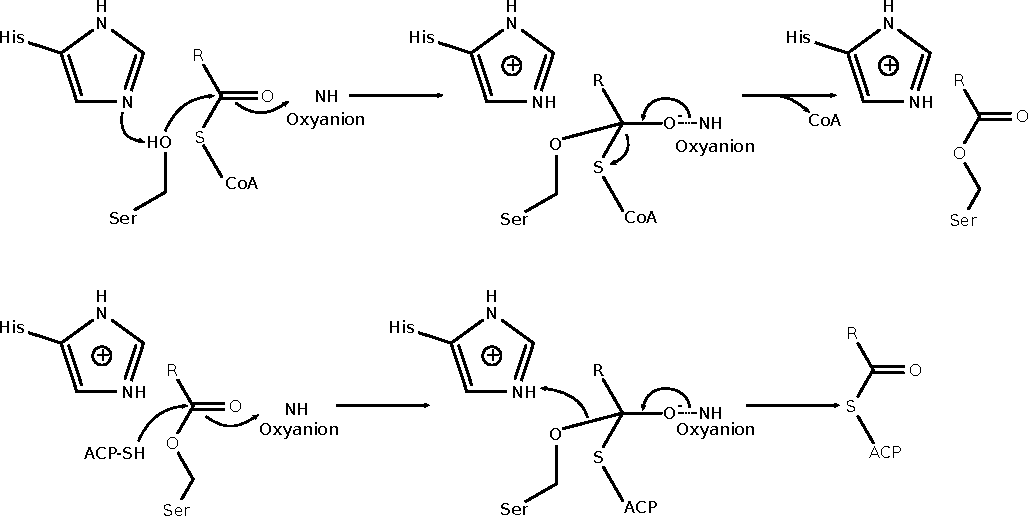
\includegraphics[width=0.95\textwidth, resolution=600, keepaspectratio=true]{graphics/ATreact.pdf}}
			\caption[Proposed reaction mechanism of AT domain]{Proposed reaction mechanism of AT domain. Figure adapted from \parencite{Smith2007}.}
			\label{fig:ATreact}
			\end{figure}
			
			Although the ATs from type I and II PKS and FAS share the same catalytic reaction mechanism and protein fold exhibit a wide range of tolerance and specificity towards the starter and extender units they transfer on the ACP. \textit{In silico} and mutagenesis experiments have identified conserved motifs within the vicinity of active site serine which determines the specificity towards the different substrates. The loading domains in the \textit{cis}-AT systems were found to have more tolerance for a greater variety of starter units such as acetyl, propionyl, isopropionyl than the AT domains responsible for loading the extender units such as malonyl and methyl manlonyl \parencite{Lau1999a,Liou2003}. 
			
			The X in the GHSXG motif, which is usually a branched amino acid such as valine or isoleucine in the malonyl specific ATs, is either a glutamine or methionine in the methyl malonyl specific ATs \parencite{Haydock1995}. On comparing AT structures from DEBS AT5 with a mammalian FAS AT, DEBS AT5 has a glutamine at the X position which makes it specific for methyl malonyl extender unit, whereas mammalian FAS AT has a valine or leucine at the X position which makes it specific for malonyl extender unit \parencite{Tang2006}. 
			
			In another study, \textcite{Yadav2003} studied 187 AT sequences from 19 type I modular PKS clusters and predicted motif QQ\textbf{GHS[QMI]G}RSHT[NS]V was responsible to confer specificity towards methyl malonyl substrate and QQ\textbf{GHS[LVIFAM]G}R[FP]H[ANTGEDS][NHQ]V motif was associated with malonyl specificity. They have also identified a position R117 in \textit{E. coli} malonyl-CoA:acyl carrier protein transacylase crystal structure (PDB ID 1MLA) which was conserved in all the malonyl and methyl malonyl specific ATs but changes to a non polar amino acid for the ATs specific for monocarboxylic substrates such as propionate. These motifs are embedded in their PKS domain detection program SEARCHPKS \parencite{Yadav2003a}. Another motif is the YASH motif which contains the catalytic histidine 100 residues downstream of the catalytic serine. YASH motif was found to be specific in the methyl malonyl specific ATs whereas HAFH at the same position was specific for the malonyl substrates \parencite{Haydock1995}.  
			
			\subsubsection{Ketosynthases (KS)}
			\label{sec:KS}			
			Ketosynthases are responsible for catalysing Claisen condensation in PKS, FAS and NRPS systems. KSs belong to the thiolase family of proteins and in type I FAS and type I and III PKS they form homodimers \parencite{Austin2003, Tang2006}. KSs in type II PKS also forms the dimer but only one subunit performs the Claisen condensation and the second subunit which is also known as chain length factor is a non functional KS considered to be responsible for keeping a check on the growing polyketide chain length \parencite{Tang2003, Szu2011}. The homodimeric state in type I PKS and FAS is considered to be the primary factor for the dimerization of the two subunits. Although ER and DH domains are also found to form dimers, experiments have shown that upon KS deletion the FAS subunits fails to dimerize \parencite{Smith2007}. The thiolase fold of the two dimer forming KSs follow the same  alternating $\alpha /\beta/ \alpha/ \beta/ \alpha$ architecture. The active site is formed at the dimer interface by the contribution of the residues from both the subunits. The active site can be viewed as two segments, one at the most buried segment is next to the dimer interface and bind the acyl intermediate, and an outer tunnel starts from the enzyme surface and binds the phosphopantetheine arm. Sequence analysis has shown diversity and lesser sequence similarity in the residues lining the acyl intermediate binding pocket as compared to the phosphopantetheine binding tunnel \parencite{Olsen2001}. This is due to the ability of the KS across different systems to accept a variety of substrates which are however, attached to the same phosphopantetheine arm. 
			
			There are two main classes of Claisen condensations for carbon-carbon bond formation; the decarboxylating and the non-decarboxylating. The structures of the KSs used for both the classes are low in sequence similarity but still have the same three dimensional thiolase fold \parencite{Heath2002}. The decarboxylating condensing enzymes can be further divided into two sub classes based on the primary sequence analysis 1) Initiation ketosynthase such as type I FAS, FabH  and 2) Elongation ketosynthases such as type I FAS, FabB and FabF \parencite{Davies2000}. The initiation enzymes utilize CoA substrate as the primer whereas the elongation enzymes utilize ACP thioesters however, the reaction mechanism followed by both the enzymes is same. The initiation ketosynthases as the name suggests are found at the beginning of the type I FAS and PKS usually in the loading module for example the niddamycin pathway \parencite{Kakavas1997}.
			
			After years of disagreement and research and with the availability of the high resolution crystal structures of KSs from both FAS and PKS systems researchers have come to the consensus that the Claisen condensation is a three step process involving a CYS-HIS-HIS catalytic triad (Figure \ref{fig:KSreact}). In the \textit{E. coli} FAS (FabB/FabF) KS (PDB ID 1DD8) C163, H298 and, H333 forms the catalytic triad (Figure \ref{fig:KS}). The Claisen condensation initiates with the acyl chain transfer from an ACP on to the catalytic cysteine forming an ACP-acyl-KS thioester tetrahedral intermediate. In FAS (FabB/FabF) this tetrahedral geometry is stabilized by the backbone amides contributed by the catalytic cysteine and a glycine (G391). The pKa of a free cysteine (8.0 to 8.8) is not sufficient for the deprotonation and the nucleophilic attack on the acyl carbonyl. A pKa of about 7.0 or lower is required for the cysteine to act as a nucleophile under physiological conditions. \textcite{Qiu1999} suggested H244 may be involved in assisting the deprotonation of the cysteine thiol. However the distance between the N $\epsilon$ ans S $\gamma$ of the H244 and catalytic cysteine respectively were too far for this to happen. Furthermore replacement of H244 with an alanine resulted in a protein that was unable to catalyse the complete condensation reaction, but was 6 times faster in transacylation than the wild type. However, mutagenesis studies on H244 do show that it assists in the deprotonation of the thiol at low pH \parencite{Davies2000}. The probable explanation for the deprotonation of the catalytic cysteine thiol under physiological conditions was given on the basis that the cysteine is present at the N-terminus of the alpha helix, the positive end of the dipole moment of the helix could stabilize the negative charge, allowing transfer to the acyl chain to the cysteine \parencite{Davies2000}.

			\setlength\fboxsep{5pt}
			\setlength\fboxrule{1.5pt}
			\begin{figure} []
			\centering
			\fbox{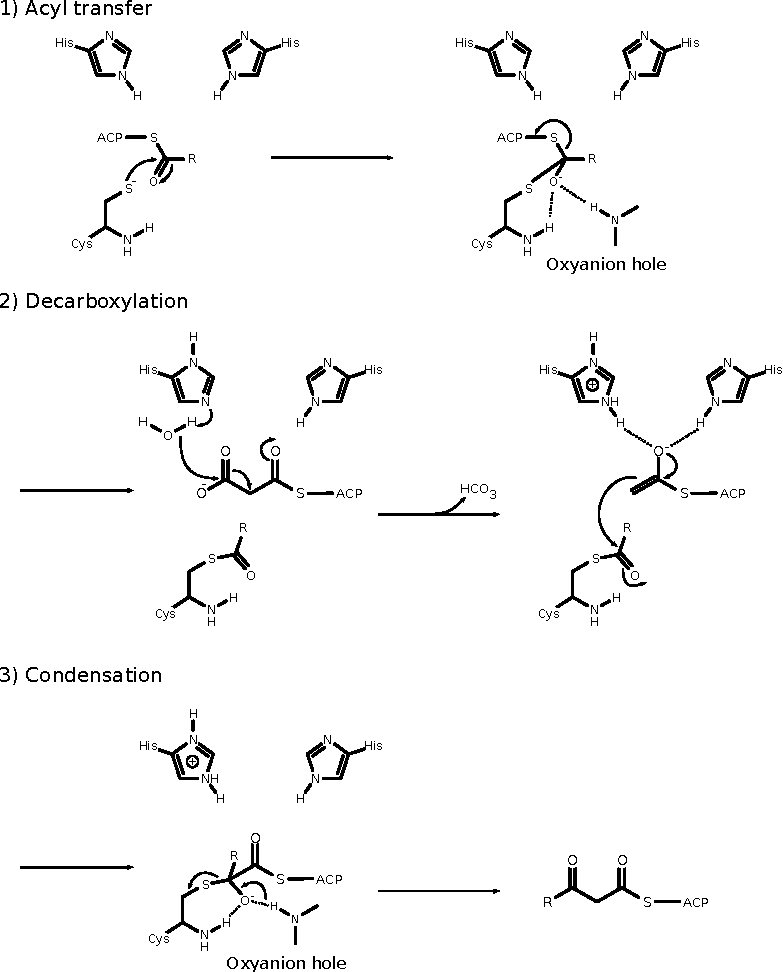
\includegraphics[width=0.95\textwidth, resolution=600, keepaspectratio=true]{graphics/KSreact.pdf}}
			\caption[Proposed reaction mechanism for Claisen condensation]{Proposed reaction mechanism for Claisen condensation. Figure adapted from \parencite{Smith2007}.}
			\label{fig:KSreact}
			\end{figure}			
						
			\setlength\fboxsep{5pt}
			\setlength\fboxrule{1.5pt}
			\begin{sidewaysfigure} []
			\centering
			\fbox{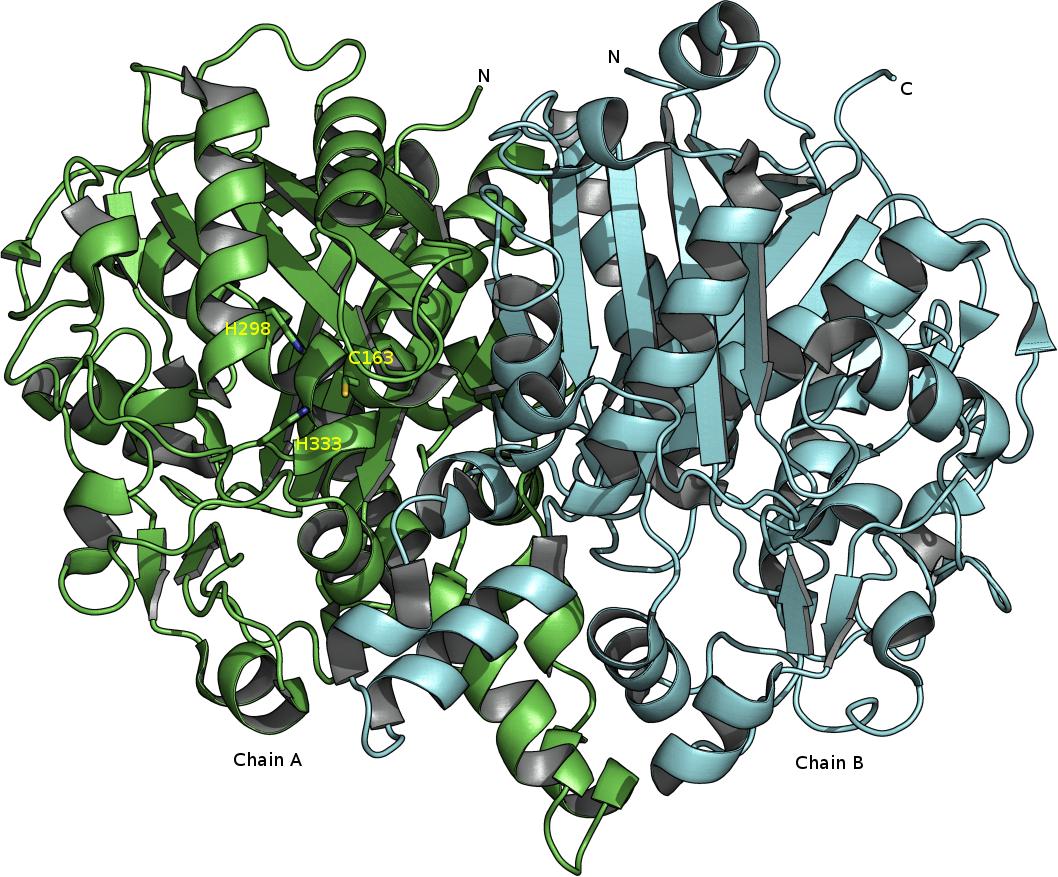
\includegraphics[width=0.7\textwidth, keepaspectratio=true]{graphics/ks.png}}
			\caption[Cartoon representation of a ketosynthase homo dimer from FAS in \textit{E. coli}]{Cartoon representation of a ketosynthase homo dimer from FAS in \textit{E. coli} (PDB ID 1DD8). The catalytic triad C163, H298 and H333 are drawn as sticks \parencite{Olsen1999}.}
			\label{fig:KS}
			\end{sidewaysfigure}
			
			The second step involves the decarboxylation of the malonyl extender unit attached to the ACP. The two histidines are considered to be involved in the decarboxylation of the malonyl unit. A water molecule in the active site is thought to be activated by one of the histidines which in turn attacks the C3 carbonyl of the malonyl resulting in the formation of an enol intermediate, stabilized by the histidines. This decarboxylation step also happens in the absence of the acyl-cysteine thio ester and that is why the above mentioned initiation keosynthases that lacks catalytic cysteine are able to decarboxylate a malonyl or methylmalonyl units into an acetyl or propionyl units respectively. Such initiation ketosynthases carry a glutamine in place of a cysteine (also known as $ KS^{Q} $). In the final step the enol intermediate forms a carbanion which in turn attacks the acyl-cysteine thio ester resulting in a tetrahedral intermediate which is again stabilized by the oxyanion hole followed by the release of the acyl-ACP \parencite{Heath2002}. 
			
			In modular \textit{cis}-AT PKS, Ketosynthases have shown to be tolerant in terms of substrate specificity and can readily accept non native substrates. Studying the structure of the type I and type II KS, type I KSs have a loop at the interface in the homodimers which is replaced by a helix in the type II KSs. This loop region is hypothesized to be responsible for providing additional space to accommodate non native substrate which otherwise is restricted by the helix in the type II KSs \parencite{Pan2002}. KSs were able to catalyse chain elongation with inactivated KR5 or ER4 domain in the DEBS system. KS2 in the DEBS system was also found to be tolerant towards several substrates \parencite{Khosla1999}. Using a KS1 knockout strain  \textcite{Khosla1999} showed that (2S,3R)-diketide  and analogous substrates attached to a NAC molecule tolerated and processed by the KS2 domain. Not only different variants of diketide moeities they also tested an anhydro-triketide moiety which was able to be processed by the KS2, these substrate variants produced analogues of 6-DEB molecule. As well as KS2 being tolerant towards (2S,3R)-diketide moiety KS3, KS5 and KS6 were also able to accept and produce triketide products \parencite{Khosla1999}. 
			
			Recent phylogenetic studies have shown that the \textit{cis} and \textit{trans} PKS evolved independently through different routes. The KS from the \textit{trans}-AT systems were likely to be incorporated via horizontal gene transfer as opposed to gene duplication events in the \textit{cis}-AT systems. This difference may explain how \textit{trans} AT systems came to be more specific towards their substrates as compared to their \textit{cis}-AT counterparts \parencite{Nguyen2008}. These hypothesis were also experimentally supported by the two recent collaborative papers by Piel and Oldham group. In the first paper by \textcite{Jenner2013} utilizing a newly developed mass spectrometry (MS) based method to study ketosynthases specificity analysed substrate specificity of KS5 from bacillaene and KS1, KS2 and KS3$^{0}$  from psymberin biosynthesis pathways. KS5 in the BaeL subunit resides right before the key \bet-branching step which naturally makes it tolerant for non branched substrates. Similarly KS1 and KS2 from PsyA processes non branched substrate and KS3$^{0}$ from PsyD is a non condensing keto synthase but is capable of acyl transfer. \textcite{Jenner2013} incubated these ketosynthases with different SNAC analogues containing branched and unbranched substrates and tested their ability to produce product with MS. They found that the KS5 from BaeL and KS3$^{0}$ from PsyD do not tolerate branched substrate however were able to successfully process unbranched substrates. On the other hand KS1 and KS2 from PsyA were able to process branched substrate with lowered specificity. Upon sequence analysis, homology modelling and substrate docking of KS5 of BaeL, they found that the residue right before the catalytic cysteine (X-cys) seems to interact with the \bet-carbon. This position X is usually a bulky residue like methionine in the non branch accepting ketosynthases and a smaller residue like glycine or alanine in the branched chain accepting ketosynthases. KS5 from BaeL and KS3$^{0}$ from PsyD  have methionine on that position whereas KS1 and KS2 form PsyA have an alanine, which explains the more tolerant behaviour of the branched substrate by KS1 and KS2. To test this prediction from the computational analysis \textcite{Jenner2013} created a KS5 M237A mutant and incubated it with branched and unbranched SNAC analogues. The unbranched analogues were successfully transferred onto the catalytic cysteine of the KS5 mutant as the more space created inside the active site would have not affected the binding of the unbranched substrate. However, the KS3 mutant also showed increased levels of branched substrate specificity which suggests the necessity of the space created by replacing a bulky residue with a small residue immediately preceding the catalytic cysteine. These experiments laid down the new rules for predicting the specificity of KS domains towards branched and unbranched substrates. Although this rule is only restricted to the \bet- position in the substrates authors do not deny the possibility of discrimination based on the interactions at other parts of the substrate. 
			
			In the second paper, \textcite{Kohlhaas2013} tested the specificity of the bacillaene system KS1 domain from BaeJ for amino acid derived intermediates using the same protocols as mentioned above. KS1 in BaeJ accepts a glycine derived substrate from an upstream NPRS module, to test the tolerance of KS1 for different amino acid based substrates \textcite{Kohlhaas2013} created several different full length acyl-SNAC analogues utilizing glycine, alanine and valine to generate 2-amido variants. Upon incubating KS1 with the three 2-amido variants, the glycine derived substrate was able to readily transfer to the KS1 whereas the alanine based substrate did so with lower efficiency. The substrate based on valine failed to acylate KS1. In order to accommodate the bulkier valine derived substrate \textcite{Kohlhaas2013} identified M268 and L450 as the likely residues that offer steric hindrance in the entry of the substrate. They created two mutants M268A and L450A and tested all the three amino acid derived substrates. Glycine and alanine variants were still able to acylate however, the valine variant couldn't. These differences in the acylation efficiency suggested the intrinsic incompatibility of the groups at the $ \alpha $ position. They also created SNAC analogues to test any long range interaction beyond the \bet-position in the intermediates and the affect of not incorporating amide from an $ \alpha $ amino acid. There were no acylation observed in the substrate created to test the long range interaction as well as for the amide from the non $ \alpha $ amino acid. Two other acyl-SNAC analogues featuring 2-amino and 4-keto groups were also incubated to test for acylation efficiency. 2-amino SNAC  was able to acylate efficiently however, no observable acylation occurred with a 4-keto SNAC substrate. These observations suggested the need for an NH at the 2nd position, which would act as an efficient hydrogen bond donor, and that there is no requirement of the 4th carbonyl for the successful acylation. 
			
			\textcite{Kohlhaas2013} also tested KS1 for the effect of different residue type N-terminal to the catalytic cysteine on KS1's ability to accept different substrates. Through sequence analysis they found that most of the amino acid accepting KSs posses an asparagine residue at the position before the catalytic cysteine along with a few occurrence of alanine. On comparing with other ketosynthases in either \textit{cis} or \textit{trans}-AT systems they could never find an asparagine at that position. The dominating presence of an asparagine residue suggested its likely involvement in the acylation of the 2-amidoacetly substrate to KS1. To test this hypothesis they created an N206A mutant and incubated with 2-amidoacetly-SNAC. The mutant strain showed much lowered acylation efficiency. 
			
			\subsubsection{Ketoreductases (KR)}
			\label{sec:KR} 
			Ketoreductases are enzymes responsible for reducing the \bet-keto group to hydroxyl in FAS and PKS systems with the involvement of NADPH as the reducing agent. Unlike KSs which need to exist as a homodimers to function, KRs exist as functional monomers in the PKS dimer. KRs are thought to be responsible for the formation of most of the chiral centres in Polyketide products. 
			
			The stereo specificity of the products of KR domains was verified through domain swapping experiments with the KR2 from the DEBS system and the KR2 from the rapamycin system. The KR2 in the DEBS system produces an L-\bet-hydroxyl group whereas the KR2 from the rapamycin system is responsible for a D-\bet-hydroxyl group. In a model system using DEBS1 (Figure \ref{fig:DEBS}) and the DEBS thioesterase, domain swaps from rapamycin KR2 to DEBS KR2 produced a triketide with a D-\bet-hydroxyl group, confirming the stereo specificity of the KS product \parencite{Cortes1995}. It should also be noted that the mammalian FAS are known to produce D-\bet-hydroxyl groups whereas DEBS KRs produce an L-\bet-hydroxyl group, this observation also suggests that the KRs are not only responsible for the \bet-keto reduction but also for assigning the correct stereo chemistry to the resultant hydroxyl group \parencite{Kao1998}. KRs from the DEBS systems were also found to be tolerant of different substrates. In a domain swap experiment, a system with KR5 from the DEBS system replacing KR2 successfully produced the DEBS1 triketide product, suggesting a wide tolerance for KR substrate specificity \parencite{Khosla1999}.
			
			\setlength\fboxsep{5pt}
			\setlength\fboxrule{1.5pt}
			\begin{sidewaysfigure} []
			\centering
			\fbox{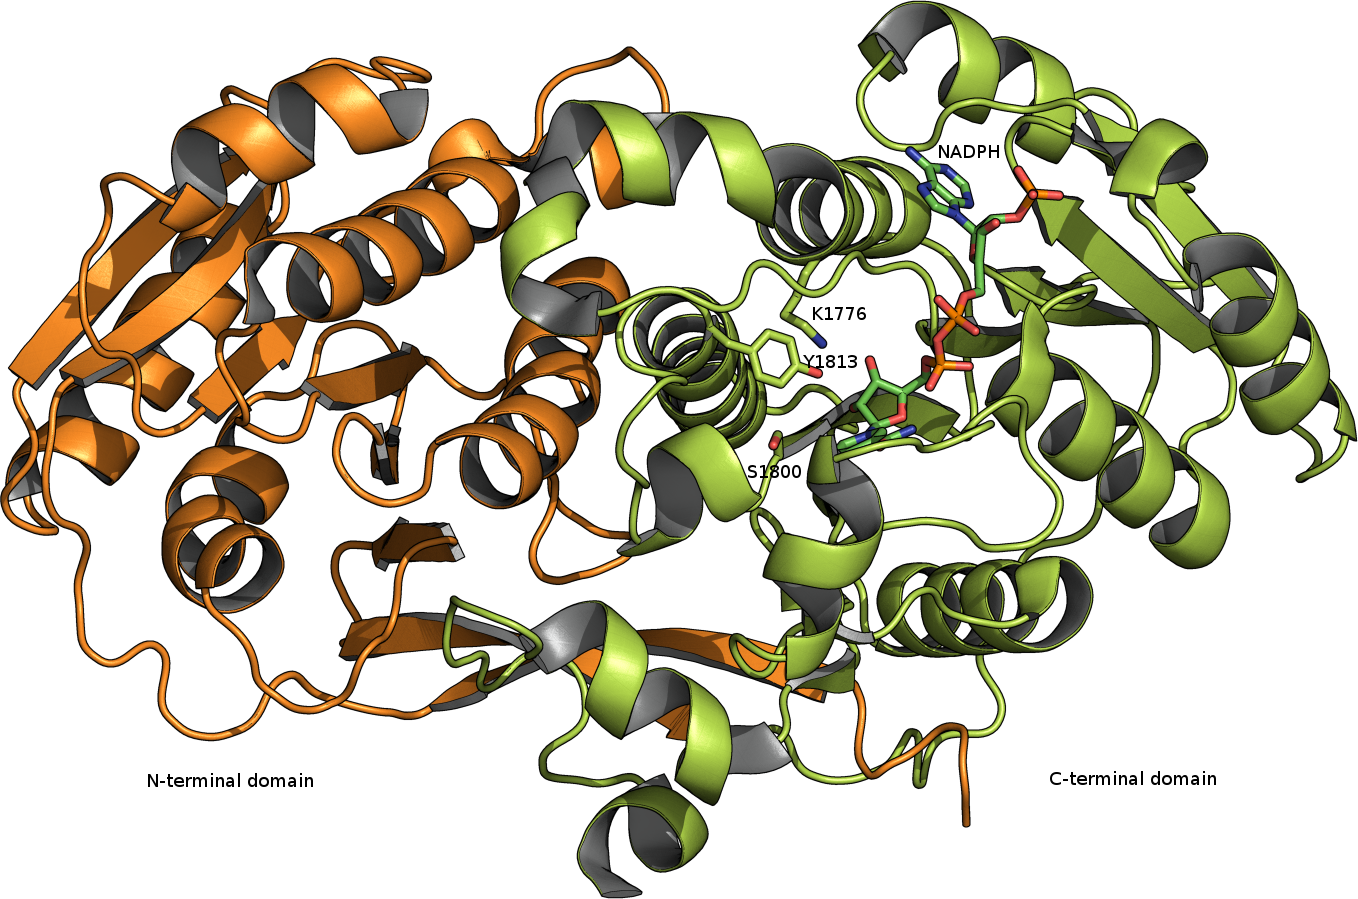
\includegraphics[width=0.8\textwidth, keepaspectratio=true]{graphics/KR.png}}
			\caption[Cartoon representation of a keto reductases domain]{Cartoon representation of a keto reductases domain from the first module of DEBS biosynthesis pathway (PDB ID 2Fr0). The N-terminal structural domain (orange) and the C-terminal catalytic domain (lime) are highlighted along with the catalytic triad Y1813, S1800 and K1776 drawn as sticks. The bound NADPH molecule is shown as sticks \parencite{Keatinge-Clay2006}.}
			\label{fig:KR}
			\end{sidewaysfigure}
			
			Ketoreductases can be classified into three types, type A which is responsible for L-$ \beta $-hydroxyl group, type B for D-$ \beta $-hydroxyl group and type C which are incapable of \bet-keto reduction. Type A and B can be further sub classified as 0, and 1 and 2 depending upon whether they reduce an un-$\alpha$-substituted substrate or an $\alpha$-substituted substrate. A0 and B0 will be type A and B which cater an un-$\alpha$-substituted substrate whereas A1, B1 accepts D-$\alpha$-substituted substrates and A2, B2 accepts L-$\alpha$-substituted substrates  (i.e. [LD]-$ \alpha $-alkyl-[LD]-$ \beta $-hydroxyl). The type C KRs can also be sub classified as C1, which are non functional, and C2, which do not perform \bet-keto reduction but are capable of epimerase activity for the $\alpha$-substituted substrates \parencite{Keatinge-Clay2007}. These classifications were made on the basis of the conserved motifs found through sequence analysis and subsequent mutagenesis and domain swap experiments \parencite{Caffrey2003, Zheng2011}. 
			
			Ketoreductases belong to the superfamily of short chain dehydrogenases/reductases (SDR) and their structures is made up of two Rossmann like fold domains for $\approx$480 residues. The N-terminal structural domain (KR$ _{s} $) does not catalyse the reduction but is thought to be important for providing correct orientation to the C-terminal catalytic domain (KR$_{ c} $). The junction of the  (KR$ _{s} $) and (KR$_{ c} $) is marked by the N-terminal $ \beta $ ($ \beta1 $) strand of (KR$ _{s} $) which is also thought to mark the boundary of the KR, forms a continuous $ \beta $ sheet with the C-terminal $ \beta $ ($ \beta7 $) strand leading to the (KR$_{ c} $) domain. Similar to the SDRs, KRs in modular polyketide synthases were hypothesized to involve the conserved catalytic triad of tyrosine, serine and lysine to carry out \bet-keto reduction \parencite{Keatinge-Clay2006, Zheng2011}. Homology modelling of KR6 from the DEBS3 and subsequent mutagenesis study on the catalytic residues proved the importance of these residues in the \bet-keto processing. \textcite{Reid2003} found that in the complete DEBS system a KR6 Y2699F mutation completely abolishes the pathway whereas KR6 K2664Q and KR6 S2686A significantly reduce polyketide production. However, in a truncated DEBS Module6+TE system all the three KR6 mutations completely abolish the triketide production. Figure \ref{fig:KR} shows the equivalent positions of the catalytic residues in the KR crystal structure from the first module of the DEBS biosynthesis pathway. In the proposed reaction mechanism for the PKS KR, similar to SDRs the catalytic tyrosine was responsible for donating the proton to the carbonyl oxygen of the substrate. Serine provided stability to the ligand through hydrogen bonds and lysine was hypothesized to lower the P$ _{k} $a of the catalytic tyrosine to assist proton transfer. All the KRs from the DEBS system were also shown to utilize pro-S hydride of NADPH. For the L and D configuration of the resultant \bet-hydroxyl group it was proposed that keeping the position of the catalytic residues and the bound cofactor (NADPH) fixed there could be two ways in which the substrate presents the \bet-carbonyl to the active sites (Figure \ref{fig:KRreact}). 

			\setlength\fboxsep{5pt}
			\setlength\fboxrule{1.5pt}
			\begin{figure} []
			\centering
			\fbox{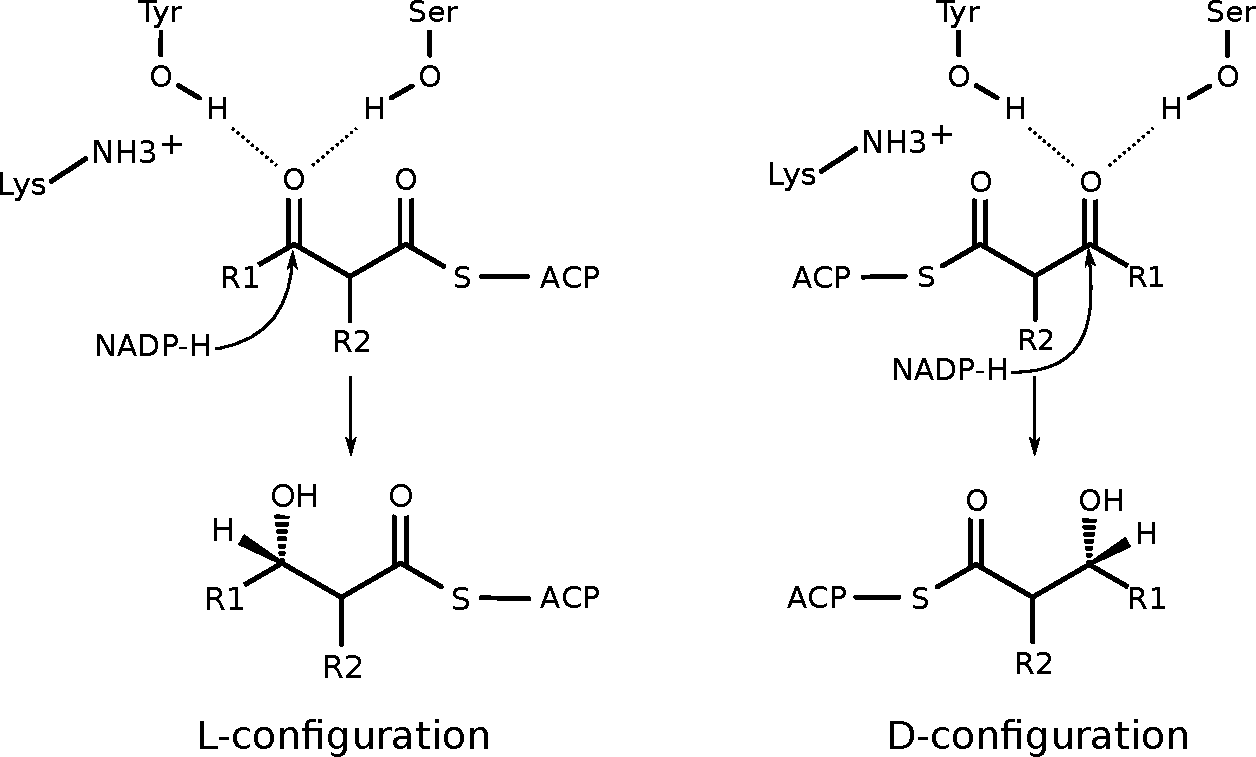
\includegraphics[width=0.95\textwidth, resolution=600, keepaspectratio=true]{graphics/KRreact.pdf}}
			\caption[Proposed reaction mechanism for \bet-keto reduction]{Proposed reaction mechanism for \bet-keto reduction. Figure adapted from \parencite{Reid2003}.}
			\label{fig:KRreact}
			\end{figure}
						
			

			\subsubsection{Dehydratases (DH)}
			\label{sec:DH} 
			DH domains catalyse the reversible dehydration of \bet-hydroxy acyl-ACP to $\alpha,\beta$-unsaturated acyl-ACPs in \textit{cis} or \textit{trans} configuration. The dehydratase domains in the bacterial FAS forms a dimer in a structural fold called a \textquotedblleft hot dog\textquotedblright (Figure \ref{fig:DH}). This hot dog fold comprises a central helix enveloped by the seven \bet-strands. In this hot dog dimeric structure there were two active sites formed at the interface in which an active site dyad histidine is contributed from one subunit and an aspartate from the other subunit. On the contrary the DHs in both the mammalian FAS and dimeric PKS (for example curacin DHs)  are formed of dimers of double hotdog folds in which the histidine and aspartate are provided by the N and C-terminal hotdog respectively (Figure \ref{fig:DH}). The orientation of the dimers in the mammalian FAS and dimeric PKS were different with respect to each other \parencite{Akey2010}. In the proposed reaction mechanism the catalytic histidine which acts as a general base helps in the removal of the proton from the $\alpha $ position and aspartate helps in the removal of \bet-hydroxyl (Figure \ref{fig:DHreact}). The stereochemistry of the dehydrated product is thought to be dependent on the configuration of the \bet-hydroxyl group \parencite{Keatinge-Clay2006, Maier2008, Akey2010}. 
			
			\setlength\fboxsep{5pt}
 			\setlength\fboxrule{1.5pt}
			\begin{figure} []
			\centering
			\fbox{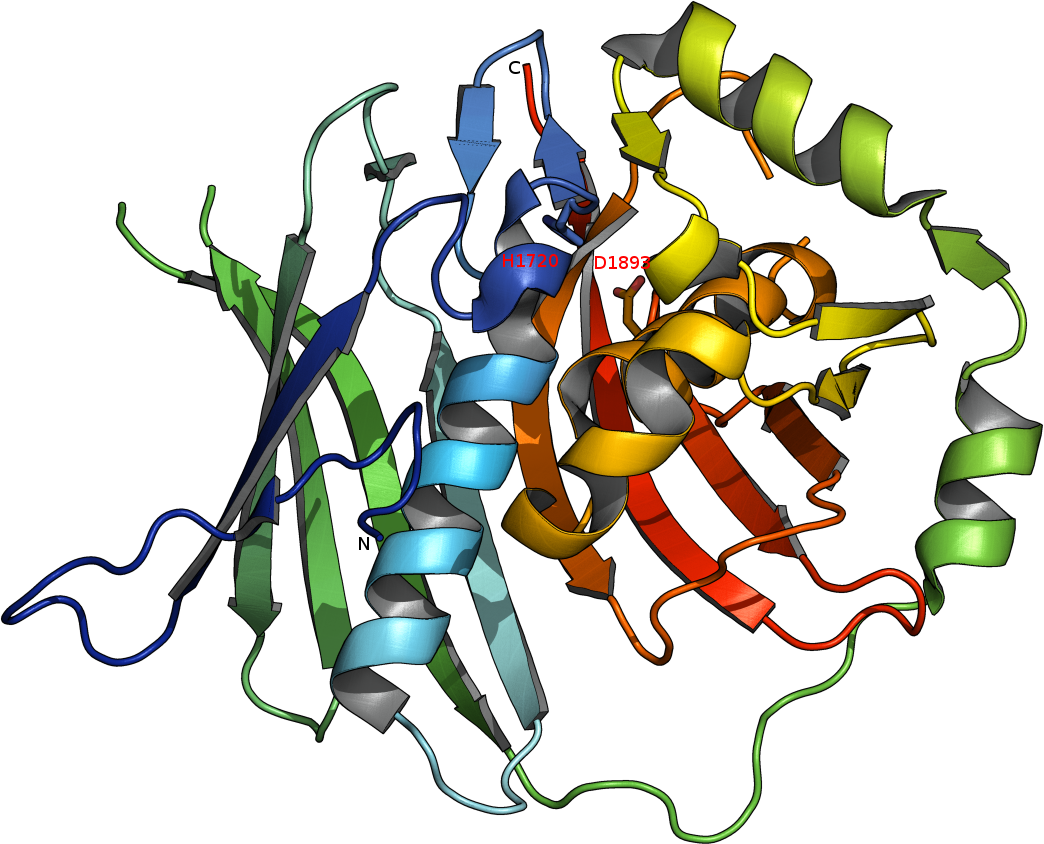
\includegraphics[width=0.95\textwidth, keepaspectratio=true]{graphics/dh.png}}
			\caption[Cartoon representation of the dehydratases domain from curacin biosynthesis pathway]{Cartoon representation of the dehydratases monomer domain (CurF PDB ID 3KG6 chain A) from curacin biosynthesis pathway. The double hot dog structure is coloured in rainbow colours with blue at the N-terminal and red at the C-terminal. The catalytic diad H1720 and D1893 are drawn in sticks and labelled \parencite{Akey2010}.  }
			\label{fig:DH}
			\end{figure}
			
			\setlength\fboxsep{5pt}
 			\setlength\fboxrule{1.5pt}
			\begin{figure} []
			\centering
			\fbox{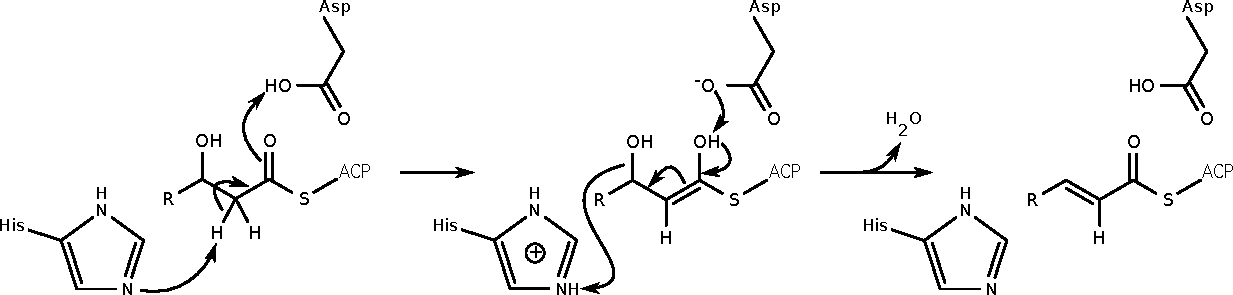
\includegraphics[width=0.95\textwidth, resolution=600, keepaspectratio=true]{graphics/DHreact.pdf}}
			\caption[Proposed reaction mechanism for \bet-hydroxy dehydration]{Proposed reaction mechanism for \bet-hydroxy dehydration.}
			\label{fig:DHreact}
			\end{figure}
			
			\subsubsection{Enoyl reductases (ER)}
			\label{sec:ER}
			The enoyl reductases (ER) in the PKS systems belong to the superfamily of MDR (medium chain dehydrogenase reductases) proteins and are responsible for the reduction of the enoyl-ACP to a fully saturated acyl-ACP on the growing polyketide molecule. These domains usually serve as the last domain in fatty acid and polyketide chain extension and modification cycle before the next round of extension begins. Most of the members of MDR superfamily including ERs exist as homo dimers or tetrameters in FASs and PKSs with the exception of the type I iterative PKS, lovastatin, which contains a free standing monomeric ER (Figure \ref{fig:ER}). 

			\setlength\fboxsep{5pt}
 			\setlength\fboxrule{1.5pt}
			\begin{figure} []
			\centering
			\fbox{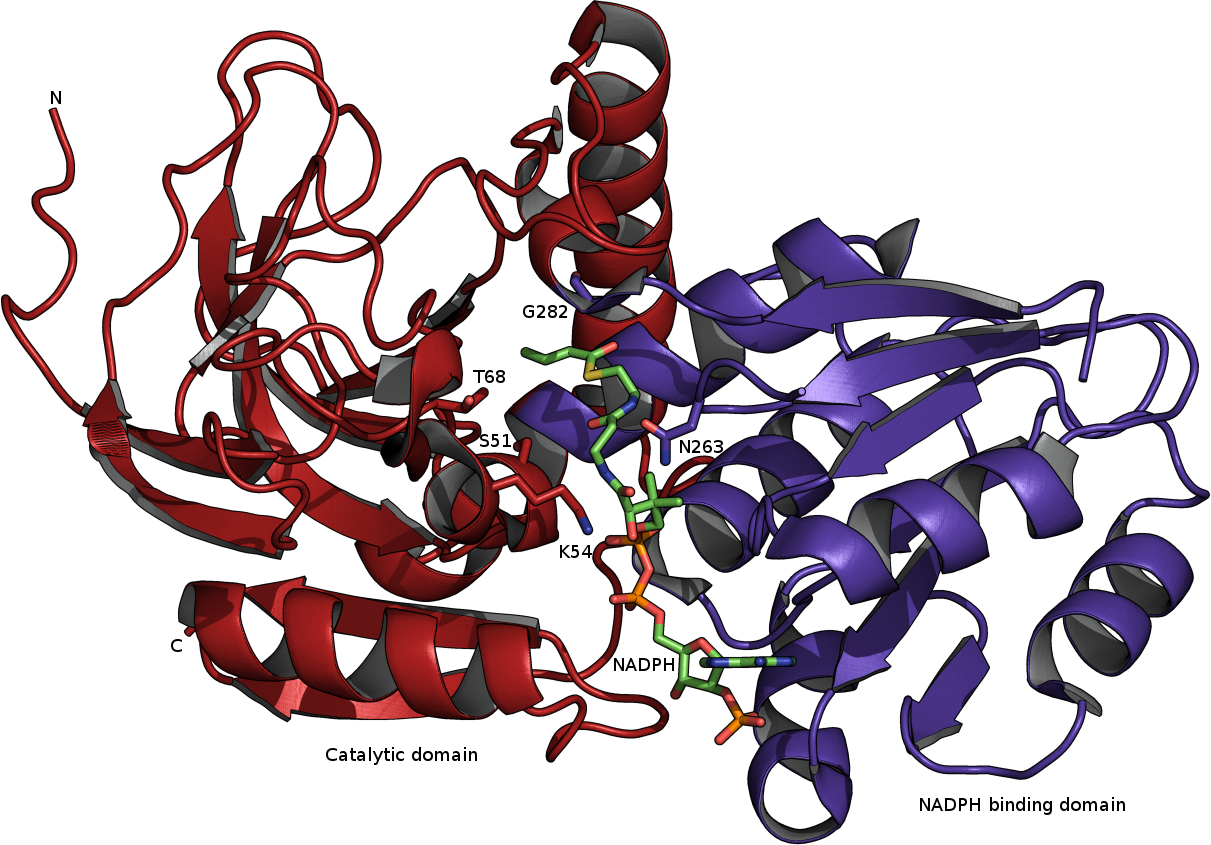
\includegraphics[width=0.95\textwidth, keepaspectratio=true]{graphics/er.png}}
			\caption[Cartoon representation of the enoyl reductase domain from the lovastatin biosynthesis pathway]{Cartoon representation of the enoyl reductase domain from the lovastatin biosynthesis pathway (LovC PDB ID 3B6Z). The catalytic domain (fire brick red) and the NADPH binding domain (purple blue) are separately highlighted. The key active site  resides  S51, K54, T68, N263 and G282 and NADPH are drawn as sticks and labelled \parencite{Ames2012}. }
			\label{fig:ER}
			\end{figure}
						
			The lovastatin ER lovC is composed of two domains the catalytic domain and the cofactor binding domain (Rossmann fold), these structural domains were also found in the other members of the MDR superfamily. The crystal structure solved by \textcite{Ames2012} and subsequent mutagenesis studies have shown key residues which are responsible for LovC catalysis. Figure \ref{fig:ER} highlights the active site residues S51, K54, T68, N263 and G282 in the LovC crystal structure responsible for the oxyanion hole formation and catalysis. In the proposed reaction mechanism (Figure \ref{fig:ERreact} ) K54 and G282 (backbone amide) participate in the oxyanion hole formation to stabilize the enolate oxide formed due to the pro-R hydride transfer from an NADPH. In the next step the enolate oxide accepts a proton most likely from a water molecule and produces a fully saturated $\alpha,\beta$-acyl-ACP. However, the ER in the type I fungal FAS is an exception to this commonly followed reaction mechanism in which the proton is not transferred by an NADPH but instead it utilizes flavin mononucleotide \parencite{Ha2006}. 
			
			The co-factor (NADPH) binding domain  can be characterised by the presence of GXGXXG / AXXXG / A motif and in the DEBS ER4, mutating the NADPH binding motif HAAAGGVGMA to HAAASPVGMA completely abolishes the ER activity. Experiments have shown that ERs have broad substrate specificity and can easily be swapped across different pathways in both FAS and PKS systems \parencite{Khosla1999, Witkowski2004a, Khosla2007}.

			\setlength\fboxsep{5pt}
 			\setlength\fboxrule{1.5pt}
			\begin{figure} []
			\centering
			\fbox{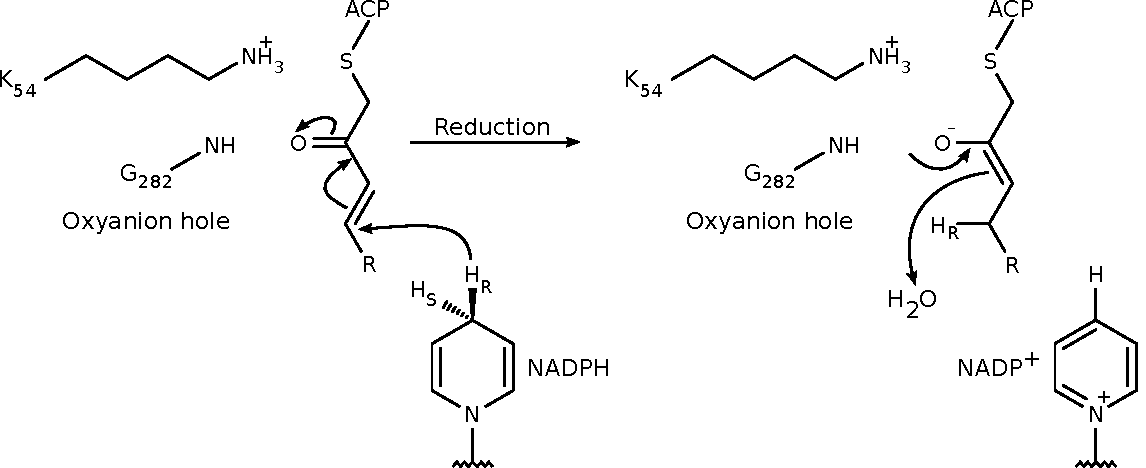
\includegraphics[width=0.95\textwidth, resolution=600, keepaspectratio=true]{graphics/ERreact.pdf}}
			\caption[Proposed reaction mechanism for enoyl reduction]{Proposed reaction mechanism for enoyl reduction in lovastatin biosynthesis pathway (LovC). Figure adapted from \parencite{Ames2012}.}
			\label{fig:ERreact}
			\end{figure}			
						
			\subsubsection{Thioesterases (TE)}
			\label{sec:TE}
			Thioesterases (TE) are the domains responsible for the hydrolytic release and sometimes macro-cyclization  of the polyketide chain attached to an ACP. In modular PKSs, TEs are usually the terminal domains however, experiments from Khosla's group have shown that TE domains are also capable of performing well when attached to a bi modular DEBS1 subunit \parencite{Gokhale1999a}. Thus, TE domains are capable of exhibiting a broad range of substrate tolerance. TE domains have a typical $ \alpha/\beta $ hydrolase fold and a S, H and A catalytic triad, both in the type I modular PKSs and type II fungal iterative PKSs. In the DEBS system the hydrolytic release of the polyketide chain has been proposed as a two step process, in the first step the catalytic S142 initiates a nucleophilic attack on the incoming polyketide intermediate resulting in the transacylation of the acyl chain to the catalytic S142 forming an acyl-enzyme complex. In the second step H259 helps to deprotonate the C-13 hydroxyl on the TE bound polyketide intermediate which results in the release and macro cyclization of the 6-deoxyerythronolide B. In the DEBS TE the 14 membered ring is also supported by seven hydrogen bonds inside the active site, which ensures the correct orientation of the C-13 hydroxyl group close to the Ser-O-acyl linkage  \parencite{Gokhale1999a, Sharma2007, Khosla2007}. Figure \ref{fig:TE} and \ref{fig:TEreact} show the crystal structure of the TE monomer from the DEBS system with the highlighted active site triad and the proposed reaction mechanism respectively \parencite{Tsai2001}. 

			\setlength\fboxsep{5pt}
 			\setlength\fboxrule{1.5pt}
			\begin{figure} []
			\centering
			\fbox{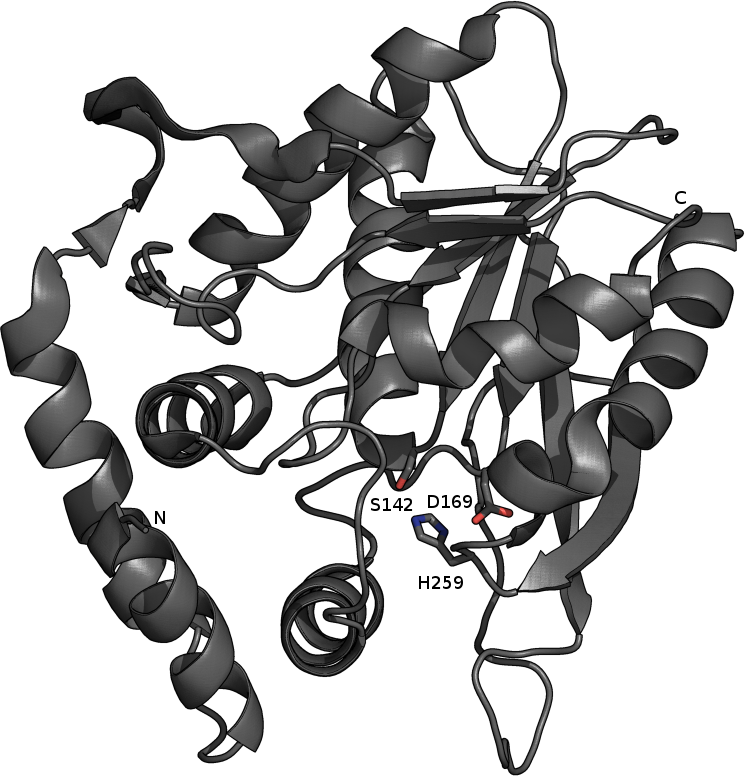
\includegraphics[width=0.7\textwidth, keepaspectratio=true]{graphics/te.png}}
			\caption[Cartoon representation of the thioesterases domain from DEBS biosynthesis pathway]{Cartoon representation of the thioesterases domain monomer from DEBS biosynthesis pathway (PDB ID 1KEZ). The catalytic triad S142, H259 and D169 are drawn as sticks and labelled \parencite{Tsai2001}. }
			\label{fig:TE}
			\end{figure}
			
			\setlength\fboxsep{5pt}
 			\setlength\fboxrule{1.5pt}
			\begin{figure} []
			\centering
			\fbox{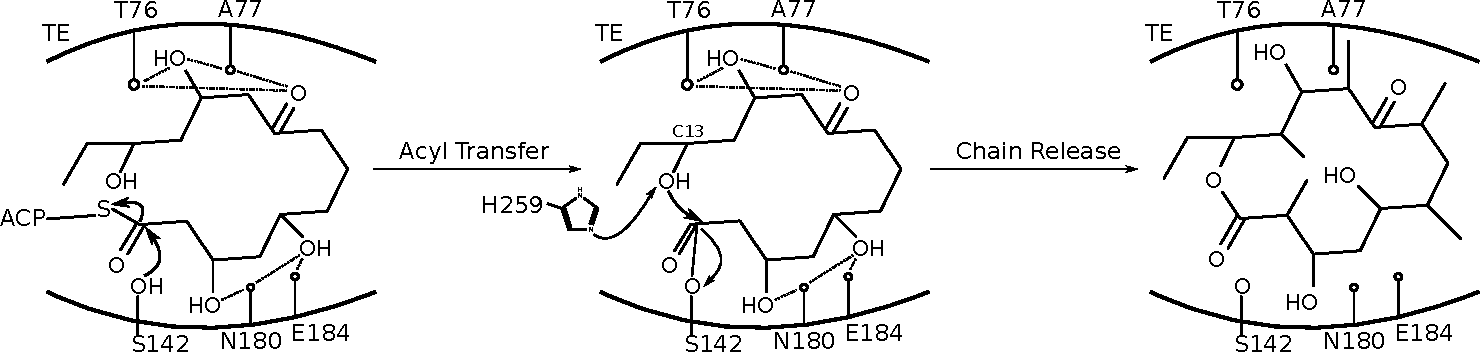
\includegraphics[width=0.95\textwidth, resolution=600, keepaspectratio=true]{graphics/TEreact.pdf}}
			\caption[Proposed reaction mechanism for thioesterase]{Proposed reaction mechanism for thioesterase in DEBS biosynthesis pathway. Hydrogen bonds are drawn as dotted lines. Figure adapted from \parencite{Tsai2001}.}
			\label{fig:TEreact}
			\end{figure}			
\newpage						
		\subsection{Complete modular structures of FAS/PKS}
		\label{sec:PKSstructure}
		The earliest attempts made to experimentally determine the complete modular structure of an FAS  were carried out in the late 1980s using small angle neutron scattering and electron microscopy using samples from chicken, pig and human FAS \parencite{Stoops1987, Kitamoto1988, Brink2002}. Owing to the poor quality of the electron density measured those models were only used to support the feasibility of the previously proposed head-to-head model over the fully extended head-to-tail model. Those models were also not good enough to correctly determine whether the two chains of the FAS were arranged in a back to back manner or were crossed over. 
		
		In the mid 2000s Nenad Ban and his colleagues were able to successfully determine the structure of a complete FAS module from mammalian and fungal species through X-ray crystallography at various resolutions \parencite{Maier2006, Jenni2007, Maier2008}. And later on in 2013 they produced a cryo-EM structure of the Mycobacterial FAS \parencite{Boehringer2013}. Similar to the previous attempts Ban's group also struggled in correctly determining the structure of the highly flexible regions such as the terminal ACP and the TE domains and it was only the yeast FAS in which they could successfully locate the position of the ACP. All the other structures were determined without the ACP and the TE domain.
		
		\subsubsection{Mammalian FAS}
		\label{sec:mFAS}
		The first crystal structure determined by the Ban group was the 4.5 \AA{} resolution mammalian FAS an  $ \alpha_{2}$-homodimeric protein with all the seven FAS domains on each of the two subunits. In spite of being successful in obtaining crystals of the porcine FAS the resolution was not good enough to correctly determine the position of the side chains in the molecule however, the secondary structural elements were clearly detectable. Therefore, they utilized the electron density map to fit the previously determined crystal structures of individual domains from type II FAS to obtain a domain architecture of the mammalian FAS (PDB ID 2CF2) \parencite{Maier2006}. 
		
		The overall shape of the mammalian FAS was like an X, imagining this as a person, the KS homodimers form the lower and DH domain pseudo dimers form the upper portion of the torso of the body, the MAT domains forming the legs attached to the KS, the ER domain homo dimer the head and the KR domains forming the arms (Figure \ref{fig:mammalianFasStructure}). This arrangement of the domains in the quaternary structure was in contrast to the linear arrangement of the domains in the primary structure and has dimensions of 210 \AA{} x 180 \AA{} x 90 \AA{}. The architecture also revealed two main dimerization interfaces, one at the KS and the other at the ER domains covering an area of $\approx$5000 $ \AA{}^{2} $. The KS dimer was found to be similar to bacterial KS I from FabB and was in agreement with cross linking experiments conducted in the mammalian FAS to cross link the N-terminus of a KS domain with the engineered active site cysteine of the other \parencite{Witkowski2004}. The ER domain homodimers form a continuous 12 stranded beta sheet at the interface joining the two nucleotide binding domains, six strands coming from each monomer. Apart from the dimer interfaces between the KS and the ER domains a small portion of the lower end of the DH domains also contribute to the overall dimer formation. The DH domains sit on top of the KS domains with the lower portion of the DH domains making a contact with the upper portion of the KS, domains which forms the waist like region. Linker regions were found in between the KS and the MAT domain and also between the MAT and DH domain. The KR domains are separate single domains hanging out as arms with no contacts between the two which was contrary to observation of tetrameric bacterial KRs \parencite{Maier2006, Boehringer2013}. 
		
		\textcite{Maier2006} made an interesting observation that the X shape of the mammalian FAS is asymmetrical. The conformation in which the X-ray structure was obtained had different sized reaction centres in the KS domain. The distance between the KRs and the MAT domains on the same sides were not similar and they were measured to be 72 \AA{} on one side and 87 \AA{} on the other. It was speculated that this difference in the size of the reaction centres may be caused by the mechanism of substrate binding to the KS and the product release after elongation, mediated by a hinge in the \textquotedblleft waist\textquotedblright \ region. In support of this hypothesis, the bacterial KSs in FabB have shown non symmetrical mode of substrate binding. They also proposed that the KS/MAT linker region might also allow the MAT domains to  move in the \textquotedblleft up and down\textquotedblright \ direction. The proposed cumulative effect of these motions were to accommodate the ACPs close to the enzymatic domains. As the observed length of the phosphopantetheine arm was only long enough for the bound substrate to reach to the centre of the active sites, implies if the ACPs were in close contact with the individual catalytic domains then there should be enough space in the quaternary arrangement of the FAS domains to accommodate the ACP next to the active site entrance of each domain.  This hypothesis also strengthened by work by \textcite{Zhang2003}, which identified the key residues responsible for the interaction between the ACPs and the KR domains in the bacterial type II FAS, thus proving the existence of domain-domain interaction between the ACPs and the FAS catalytic domains.

			\setlength\fboxsep{5pt}
 			\setlength\fboxrule{1.5pt}
			\begin{figure} []
			\centering
			\fbox{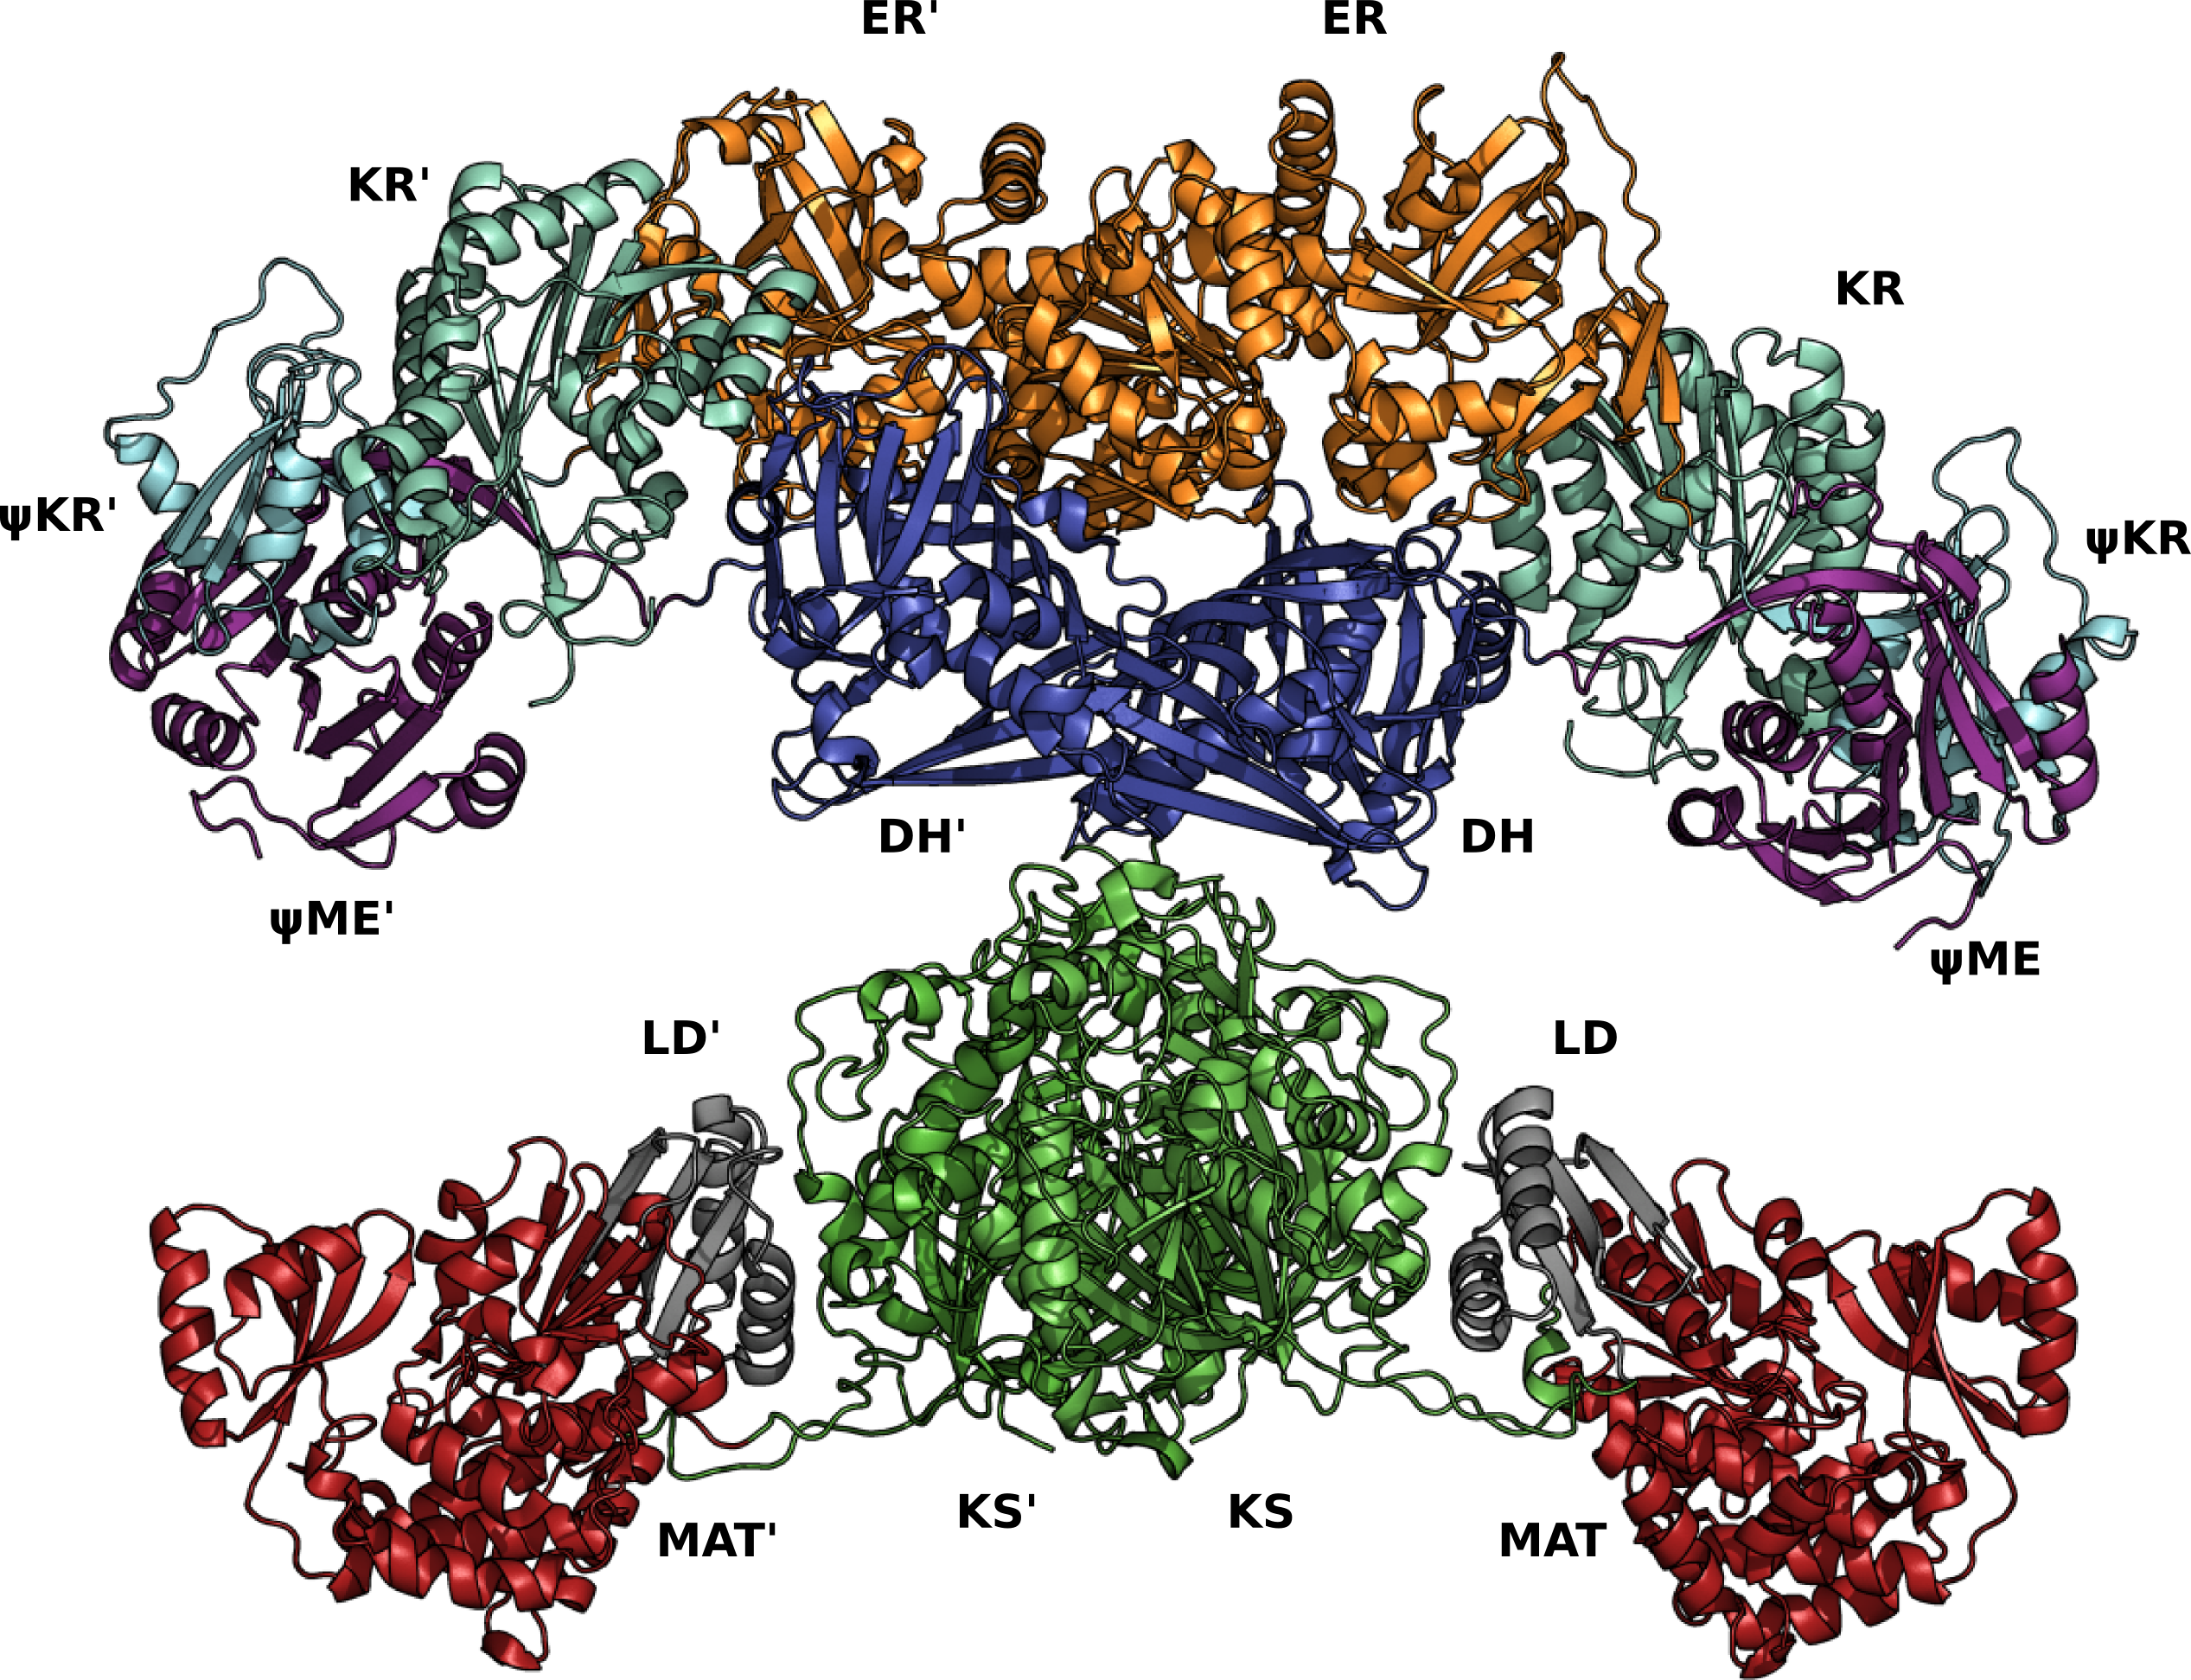
\includegraphics[width=0.95\textwidth, resolution=600, keepaspectratio=true]{graphics/mammalianFasStructure.png}}
			\caption[X-ray structure of the mammalian FAS (PDB ID 2VZ8) rendered as cartoon.]{X-ray structure of the mammalian FAS (PDB ID 2VZ8) rendered as cartoon. The catalytic (KS and MAT) and the modifying domains (KR, DH and ER) are coloured and labelled as indicated. The linker domains (LD) are coloured as grey and the pseudo domains (ME and KR) are labelled with the symbol $ \psi $.}
			\label{fig:mammalianFasStructure}
			\end{figure}			
					
		Following the determination of the mammalian FAS domain architecture based on the 4.5 \AA{} resolution X-ray crystallographic map, Ban's group successfully determined the 3.2 \AA{} resolution crystal structure of FAS in its NADP$ ^{+} $ free and bound states (PDB ID 2VZ8). The resolution for this crystal structure was good enough to correctly determine the side chains along with the secondary structure (Figure \ref{fig:mammalianFasStructure}). However, even in this attempt they couldn't determine the structure for the ACP and the TE domains. The 3.2 \AA{} resolution structure also agreed with the previously observed X shaped domain organization of the mammalian FAS. However, they identified two additional structural domains. One of the additional domains resembled a methyl transferase but is apparently catalytically inactive, and thus referred to as pseudo methyl transferase, and the other domain was similar to a ketoreductase which was thought to provide structural scaffold for the correct orientation of the catalytically active KR. This structure had similar dimerisation interfaces between the KS and the ER domains to those observed in the 4.5 \AA{} resolution model. However, the size measured was according to the electron density observed for the mammalian FAS side chains rather than the fit from the type II FAS discrete domains. The overall contact area in the dimerisation interface of the 3.2 \AA{} was measured to be 5400 $ \AA{}^{2} $ which included 150 amino acids with the contributions of $\approx$2600 and 1600 $ \AA{}^{2} $ from KS and ER domains respectively. The two DH domains also contributed 800 $ \AA{}^{2} $ to the dimerization interface along with the linker region between MAT, DH and the KS domains. This crystal structure also revealed the linker regions between the KS and the MAT domains, consisting of two helices and three \bet-strands forming an anti parallel \bet-sheet. This linker, which was thought to prevent any direct linkage between the KS and MAT domains, was also observed in the KS-AT crystal structure in the type I modular DEBS PKS determined at the same time by Khosla's group \parencite{Tang2006, Tang2007}. On the basis of the sequence context this region was also speculated to be present in the trans AT systems and a very recent crystal structure of the KS homodimers from a trans AT system showed the presence of a similar linker region attached to the C-terminal of the KS domains \parencite{Gay2014}. The precise role of this linker region is still unknown however experiments from Khosla's group have shown that they might be necessary for the ACP docking during the elongation and acyl-transfer stages \parencite{Kapur2010}. 
		
		\subsubsection{Fungal FAS}
		\label{sec:fFAS}
		In 2007 Ban group solved the crystal structure of 2.6 mDa $ \alpha_{6}\beta_{6} $ -dodecameric fungal FAS from \textit{Thermomyces lanuginosus} (PDB ID 4V58)  and that of \textit{Saccharomyces cerevisiae} (PDB ID 2UV8), both at 3.1 \AA{} resolution \parencite{Jenni2007}. The structure determined from \textit{S. cerevisiae} also revealed the position of the ACP attached to the KS active site. Although both the mammalian and fungal FAS are type I FAS where the domains are covalently attached in a single polypeptide their quaternary structures are very different from each other. The fungal FAS structure comprised of a central wheel sandwiched between two dome like structures (Figure \ref{fig:fungalFasStructure}) providing two distinct reaction centres with five entrances through the walls and top of the domes. The two reaction centres were connected by six passages through the central wheel. The central wheel was composed of 6 $ \alpha $ subunits  whereas the domes were composed of 3 $ \beta $ subunits each. One $ \alpha $ and one $ \beta $ subunit join to form a single non-redundant FAS unit. Thus in a fungal FAS complex there are six functional units of FAS formed by 12 polypeptide chains. The $ \alpha $ chains consists of KS and the KR domains and the $\beta$ chains consist of AT, MPT (malonyl/palmitoyl transferase) \nomenclature{MPT}{Malonyl/palmitoyl transferase}, DH and ER domains with numerous inter-chain contacts between the domains. All the active sites were found to point towards the inner side of the catalytic centres in the two domes. The fungal FAS also had phosphopantetheinyl transferase (PPT) domains attached to the C-terminal hanging outside the reaction centres. PPT are responsible for attaching the phosphopantetheine arm to the ACP. 
		
			\setlength\fboxsep{5pt}
 			\setlength\fboxrule{1.5pt}
			\begin{figure} []
			\centering
			\fbox{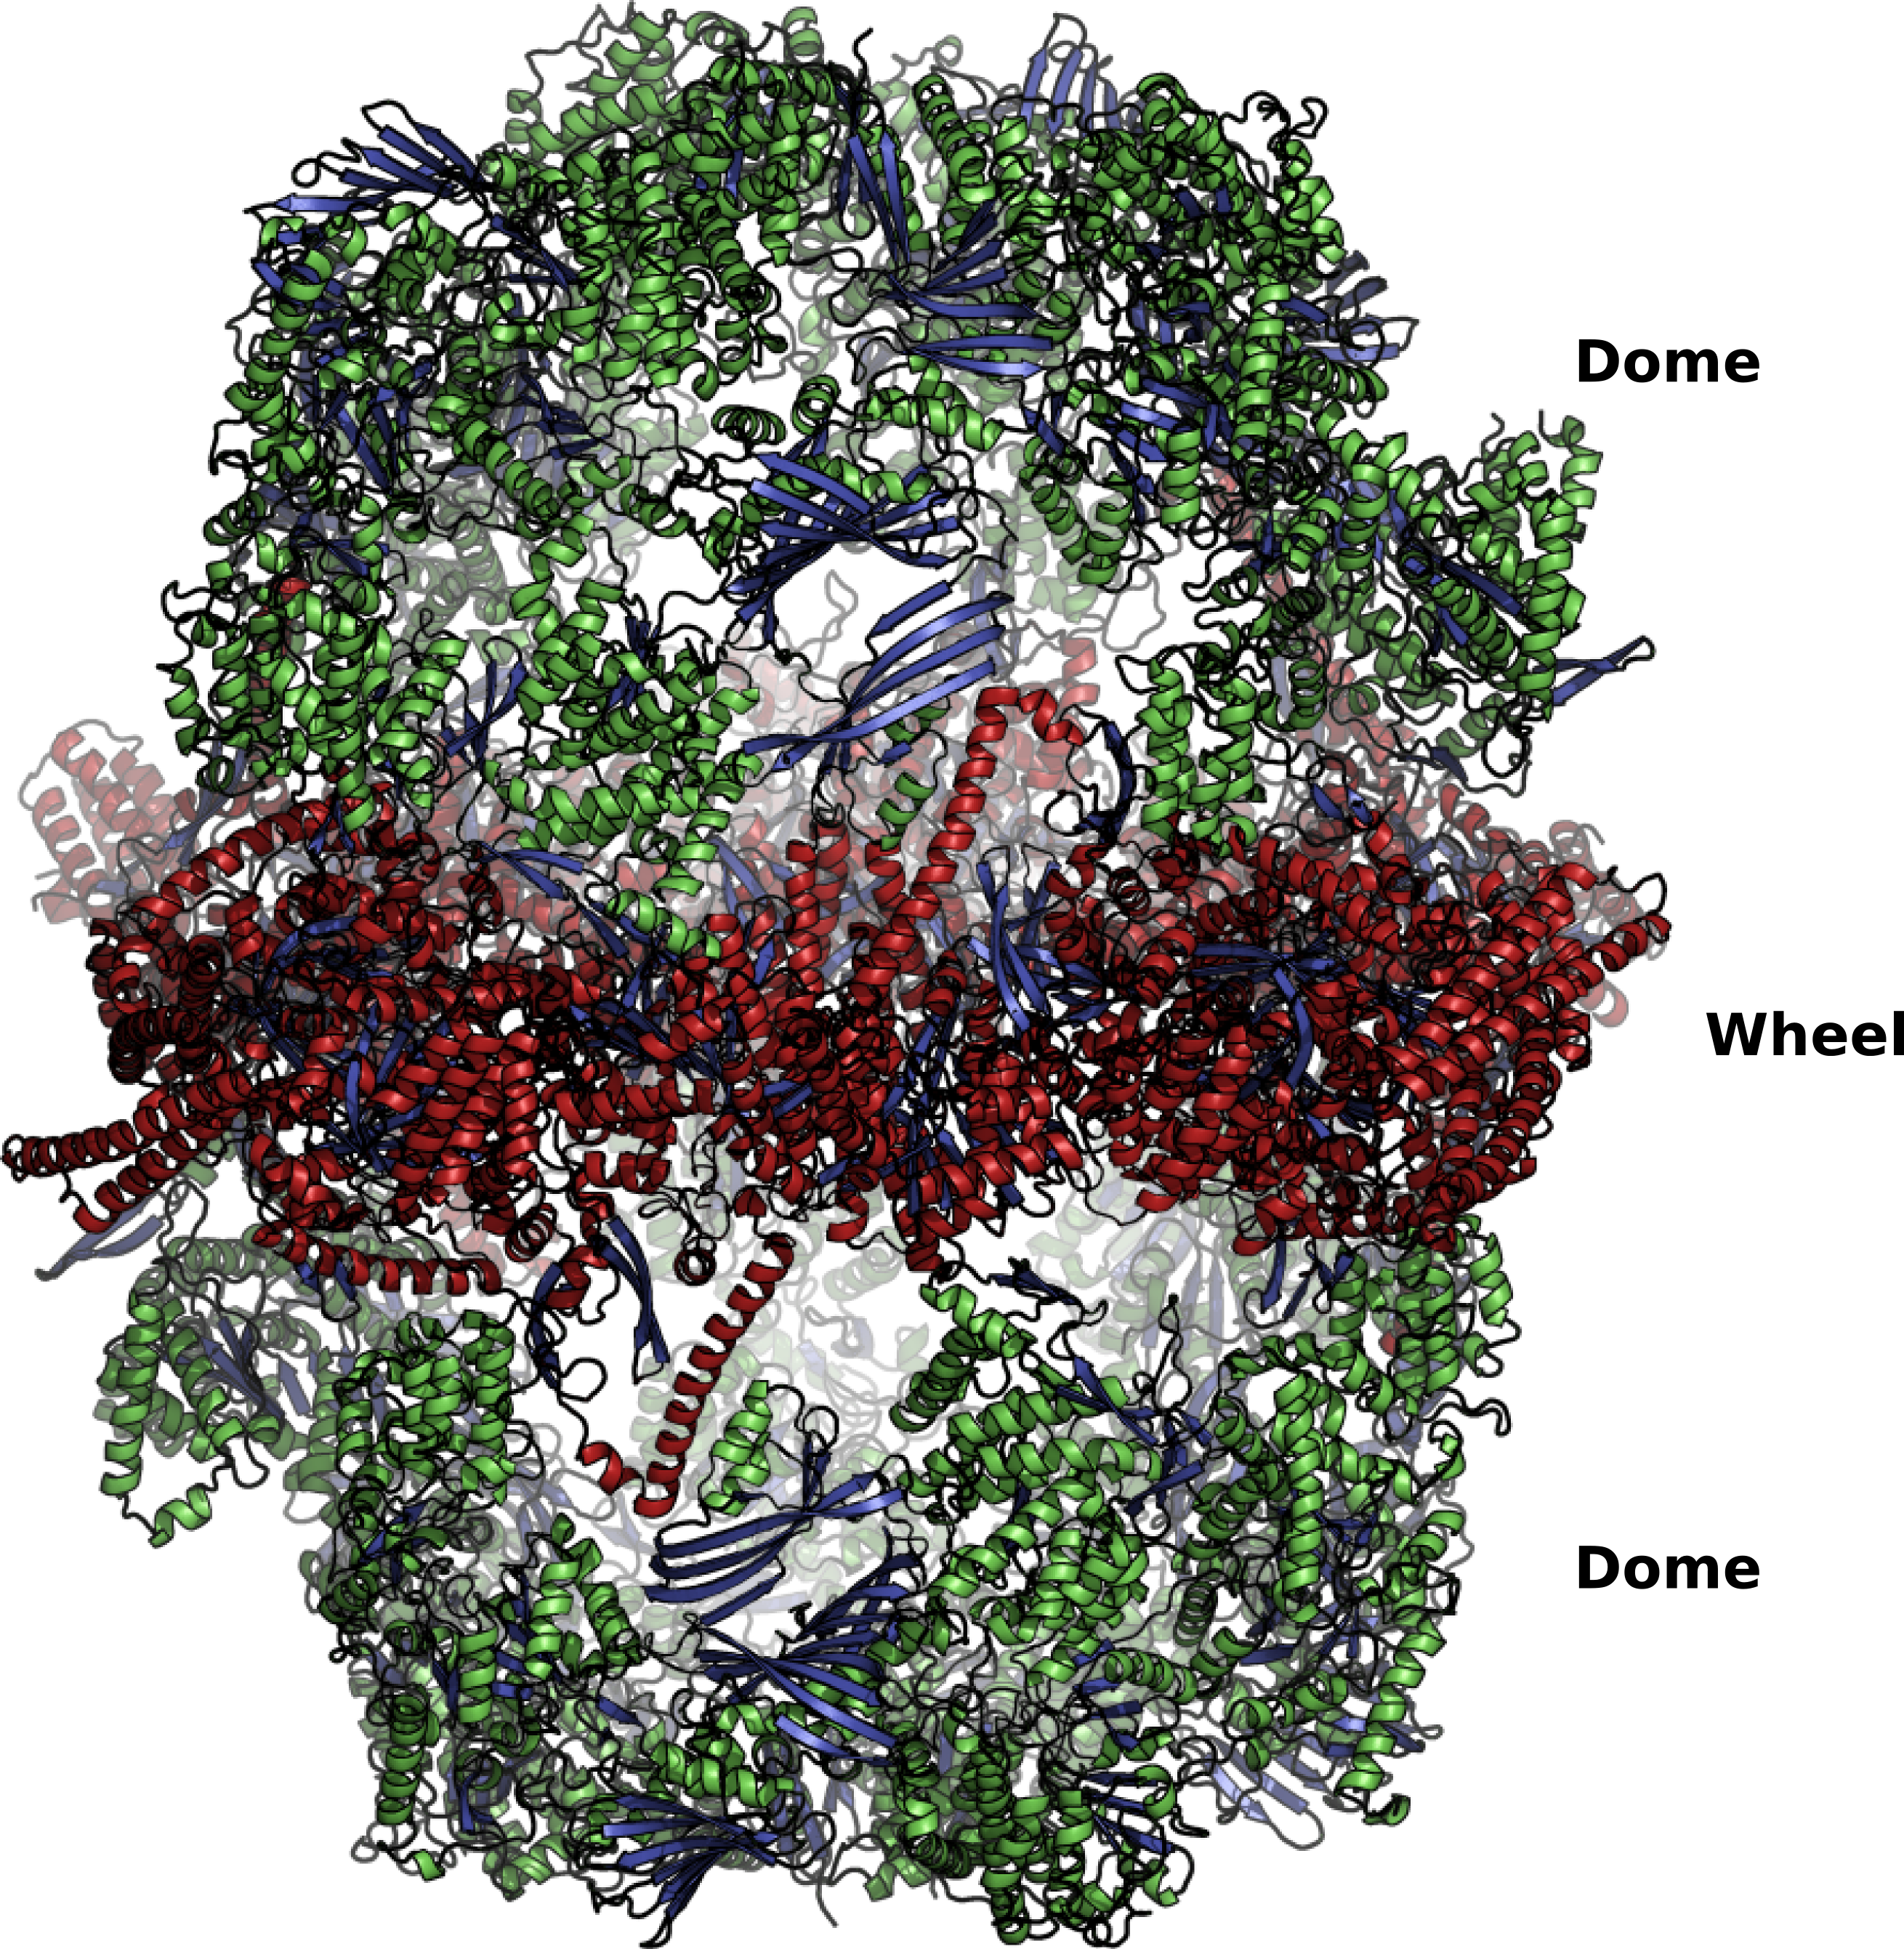
\includegraphics[width=0.95\textwidth, resolution=600, keepaspectratio=true]{graphics/fungalFasStructure.png}}
			\caption[X-ray structure of the fungal FAS (PDB ID 4V58) rendered as cartoon.]{X-ray structure of the fungal FAS (PDB ID 4V58) rendered as cartoon. Helices in the domes and the middle wheel are coloured in green and red respectively. Beta sheets are coloured in blue.}
			\label{fig:fungalFasStructure}
			\end{figure}			
		
		The all helical acyl carrier proteins in the fungal FAS were twice the size of their bacterial counterpart  with the first four helices overlapping very well with their homologues. The catalytic Serine was found to be on a loop between helices 7 and 8 whereas helix 8 was considered to be the recognition helix when making a contact with the KS. There were three ACPs each in both the reaction centres and these are doubly tethered, to the reaction centre wall at the N-terminus and to the central wheel at the C-terminus. The AT and the MPT domains had similar folds and were thought to be involved in charging ACPs with the acetyl or malonyl, and palmitoyl moieties respectively. The fungal FAS KS domains exhibit broad substrate specificity as compared to their bacterial homologues. A single FAS KS is capable of iteratively catalyse fatty acid chain elongation from $ C_{2} $ to $ C_{16} $ whereas three different KS domains are required in the bacterial FAS. All the KS domains were found to be tightly embedded in the central wheel of the fungal FAS with the active sites pointing towards opposite reaction centres. The ketoreductases found in fungal FAS followed the classical Rossmann fold however they were dimeric as compared to the monomeric mammalian and tetrameteric bacterial KRs. The DH domains in the fungal FAS formed a triple hot dog fold as compared to the mammalian double hot dog fold. The ER domains in the fungal FAS were also different from their mammalian and bacterial counterparts since the fungal ER utilizes flavin mononucleotide (FMN) \nomenclature{FMN}{Flavin mononucleotide} instead of an NADPH and forms a TIM barrel as opposed to Rossmann fold \parencite{Jenni2007, Leibundgut2007}.
		
		\subsubsection{Bacterial type I FAS}
		\label{sec:bFAS}
		In the year 2013 Ban's group published the cryo-EM reconstruction of a Mycobacterial FAS structure at 7.5 \AA{} resolution from the \textit{Mycobacterium smegmatis} species (PDB ID 4V8L, \textcite{Boehringer2013}). The Mycobacterial FAS showed a barrel shaped domain architecture similar to the fungal FAS (Figure \ref{fig:mycoFasStructure}). However, the structure was more compact with wider openings for the external entrance into the structures. \textcite{Boehringer2013} used the yeast FAS crystal structure to fit the Mycobacterial EM density map. The 7.5 \AA{} resolution was good enough to detect the individual helices however, the $ \beta $ strands were not clearly visible. Although the flattened shape of the $\beta$ sheets were detectable. 
		
			\setlength\fboxsep{5pt}
 			\setlength\fboxrule{1.5pt}
			\begin{figure} []
			\centering
			\fbox{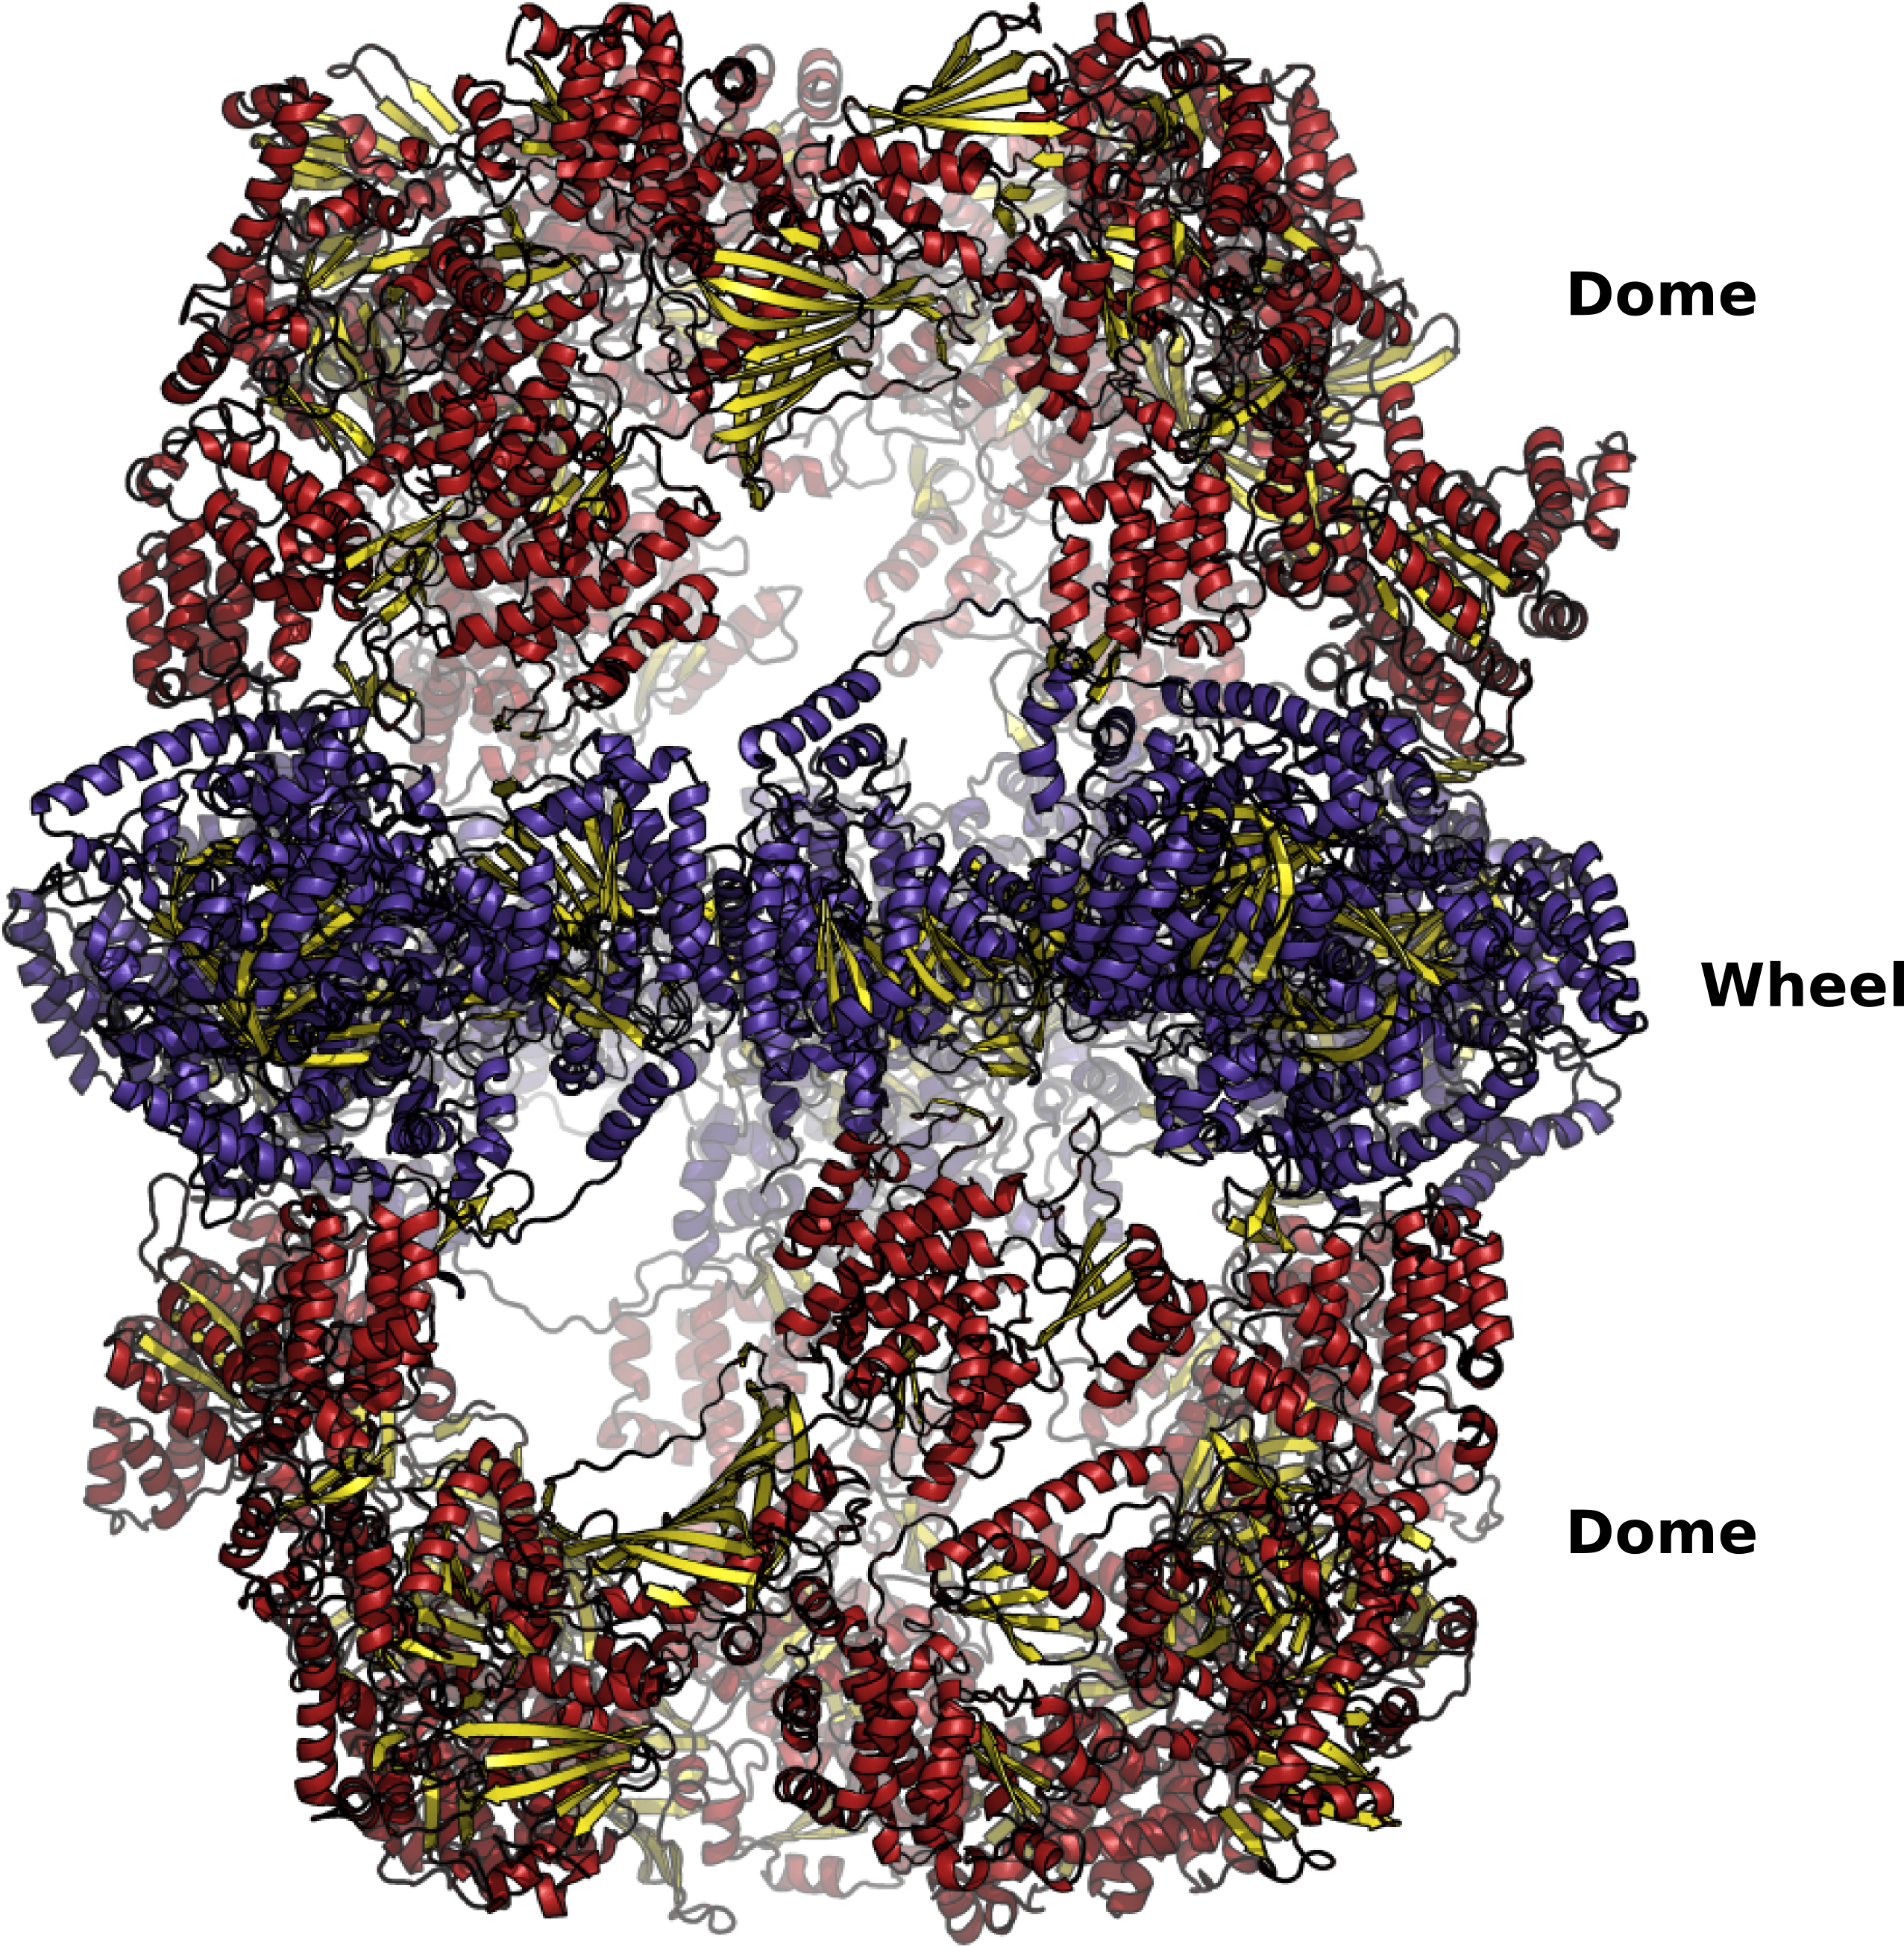
\includegraphics[width=0.95\textwidth, resolution=600, keepaspectratio=true]{graphics/mycoFasStructure.png}}
			\caption[X-ray structure of the mycobacterial FAS (PDB ID 4V8L) rendered as cartoon.]{X-ray structure of the mycobacterial FAS (PDB ID 4V8L) rendered as cartoon. Helices in the domes and the middle wheel are coloured in red and blue respectively. Beta sheets are coloured in yellow.}
			\label{fig:mycoFasStructure}
			\end{figure}			
					
		The \textit{Mycobacteium smegmatis} FAS is a 2.0 mDa $\alpha_{6}$ homohexameric structure coded as a single polypeptide containing all the catalytic domains as compared to the domains spread across two polypeptides in the fungal FAS. However, it lacked the phosphopantetheinyl transferase domain attached to the C-terminus. PPTs, called ACP synthases in \textit{Mycobacteria}, are standalone homotrimers encoded by a separate gene.This explains the presence of wider openings in the dome walls to let the ACP synthases reach the ACPs inside the reaction centres within the domes. %The AT domains in the \textit{Mycobacteria} have a conserved active site isoleucine which prevents any larger and charged substrates to be transferred on to an ACP. This suggest the role of MPT in recruiting larger substrate for the production of longer chain fatty acids.

\newpage		
		\subsubsection{\textit{Cis} and \textit{trans} AT PKS}
		\label{sec:ctPKS}
		Soon after the FAS structural elucidation by Ban's group the PKS community also released atomic resolution structural models for PKS systems. Khosla and colleagues were only able to crystallize the KS-AT homodimeric structures from DEBS 3$^{rd}$ and 5$^{th}$ modules \parencite{Tang2006, Tang2007}, and until very recently those were the only structures available for the PKS systems, which only represent part of the module. The first structure which came out was the 2.7 \AA{} resolution crystal structure of the 194 kD KS-AT homodimer from the module 5 of DEBS system (PDB ID 2HG4). This structure agreed very well with the then resolved 4.5 \AA{} resolution domain architecture structure of the mammalian FAS and was similar to the leg region of the mammalian FAS structure (Figure \ref{fig:debs2hg4tructure}). 

			\setlength\fboxsep{5pt}
 			\setlength\fboxrule{1.5pt}
			\begin{figure} []
			\centering
			\fbox{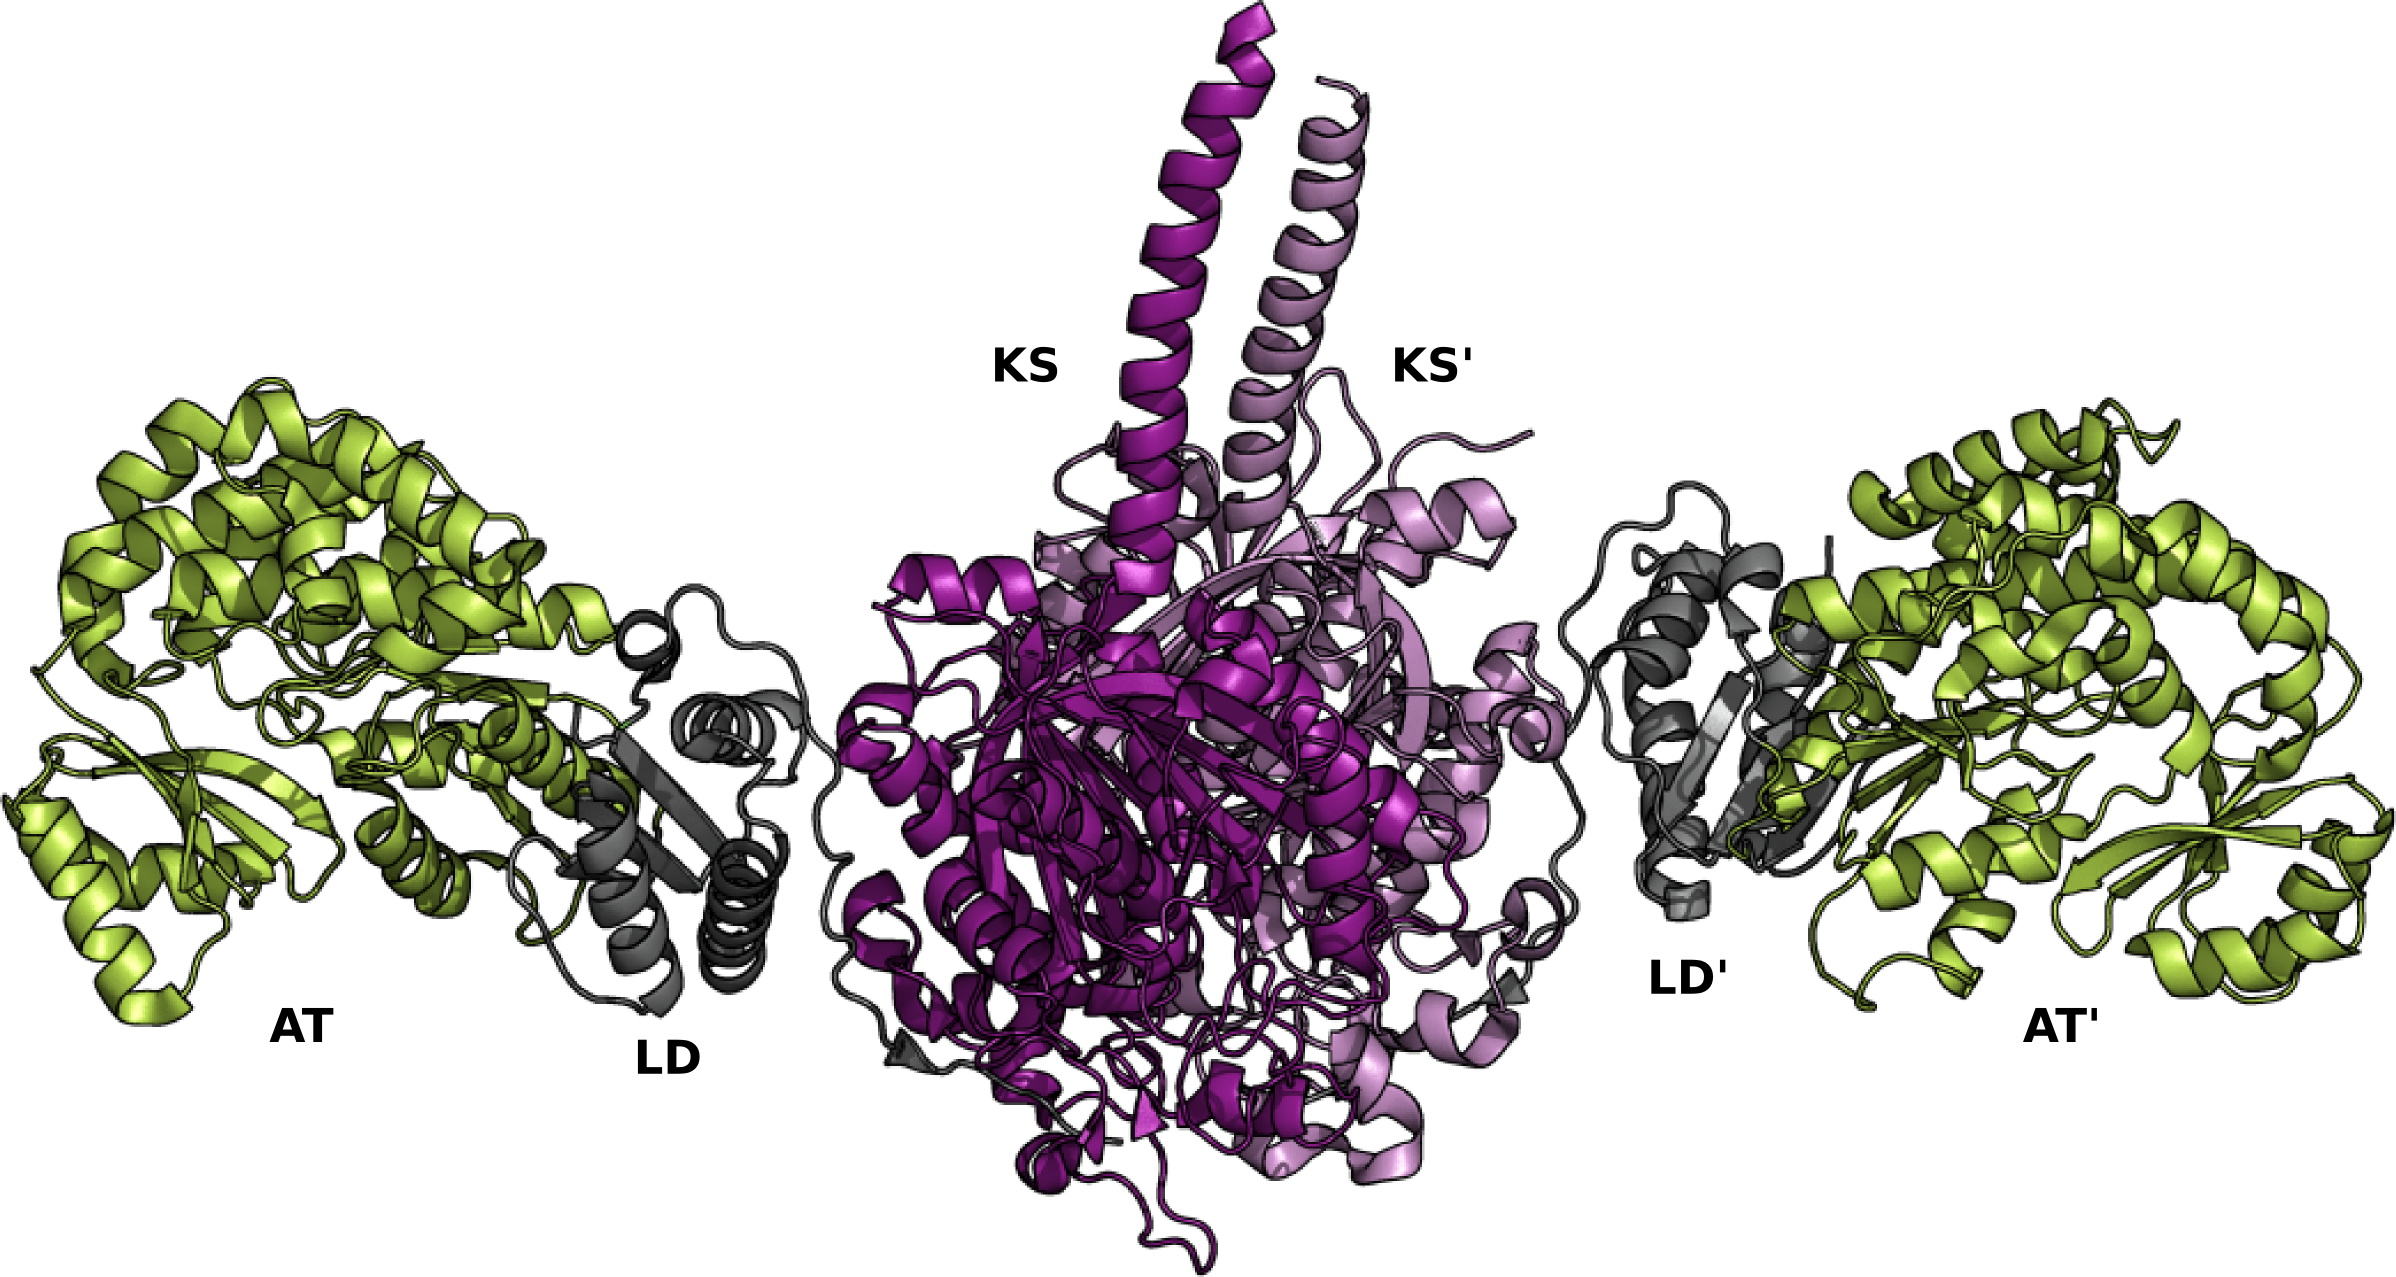
\includegraphics[width=0.95\textwidth, resolution=600, keepaspectratio=true]{graphics/debs2hg4Structure.png}}
			\caption[X-ray structure of the KS-AT homodimer from the DEBS (PDB ID 2HG4) system rendered as cartoon]{X-ray structure of the KS-AT homodimer from the DEBS (PDB ID 2HG4) system rendered as cartoon. Ketosynthase (KS) dimers are coloured in two different shades of purple, linker domains (LD) are coloured in grey and acyltransferase (AT) domains are coloured in lemon yellow.}
			\label{fig:debs2hg4tructure}
			\end{figure}					
		
		Apart from the two full length domain structures of the KS and AT domain the solved structure also had three linker regions. The N-terminal helical linker region, the linker region/domain between the KS and AT domains and the C-terminal linker which was thought to connect the AT and the KR domains. The KS domains form the dimer at the two fold axis and cover an area of 2,828 $ \AA{}^{2} $ at the interface. The KS domain fold was similar to their bacterial type II FAS counterpart and superimposed well with the \textit{E. coli} KS I domain. The N-terminal linker forms a helical dimer which protrudes outwards towards the solvent and does not make any contact with the rest of the protein complex. These linkers were thought to be involved in the inter modular interaction between the N-terminal linker of the KS domains with the C-terminal linker of the ACP from the previous module.  The two helices make hydrophobic contacts and a salt bridge between them. The well defined KS to AT linker region was formed by three $ \beta $-strands sandwiched between three $ \alpha $-helices from one side and two alpha helices from the other side contributed by the AT domains and the AT-KR linker forming an $ \alpha\beta\alpha $ fold. The C-terminus of the AT domain folds back towards the KS-AT linker and extends a further 30 aa extend across the surface of the KS, which presumably forms the linker between the AT and the KR, making 8 hydrogen bonds with the KS domain and 5 hydrogen bonds with KS-AT linker. Such a fold was not previously reported in the PDB. 
		
		Similar to the KS domains, AT domains also had the similar fold to that of the bacterial type II AT domains and superimposed well with the \textit{E. coli} AT domain, with the RMS deviation of 1.59 \AA{}. This structure also revealed an $\approx$80 \AA{} distance between the active site C199 and the S642 in the KS and AT domains respectively which suggested an extensive movement of the ACP domains in substrate channelling that would otherwise not be possible just by the phosphopantetheine arm of $\approx$20 \AA{}. 
		
		The active site of the KS domains also matched well with their bacterial type II homologues where it centres around the active site Cysteine reaching towards the dimer interface. The active site cleft was formed by the contribution of the residues from both the subunits and was connected via a tunnel to the outer opening at the surface of the KS domain. The residues lining the tunnel were highly conserved among the KS's homologue with the primary role of supporting the phosphopantetheine arm. Another interesting observation made through the KS-AT homodimer structure was the flexible loop region (residue 153-161) at the dimer interface which forms the part of the active site. This loop region is a helix in the type II KSs. It was hypothesized that this loop might be responsible for the KS specificity and helps in accommodating substrates of different size. This observation agreed well with the previous observations that the KS 5 can accommodate substrates of larger size than the native ligand \parencite{Tang2006}.
		
		The second structure solved by Khosla and colleagues was the 190kD KS-AT homodimer from the DEBS module 3 (PDB ID 2QO3, \textcite{Tang2007}). The overall fold of this strcutre was similar to the previously determined KS 5 structure however, it lacked the N-terminal linker region. The KS3 domain overlapped with the KS5 domain with an RMS deviation of 0.85 \AA{} for 386 backbone C$_{\alpha}$ atoms. One obvious difference was observed between the two KSs in the region from residue 71 to 91 (number according to KS3). This loop region on the surface in KS3 was longer as compared to the equivalent region in KS5. Sequence alignment with the other KSs from the DEBS system revealed that all the other KSs in the DEBS system were longer than KS5 by 12 residues in this region. 
		
		The KS-AT linker/domain in the KS3-AT3 structure also superimposed well with the KS5-AT5 linker region with an RMSD of 1.54 \AA{}. \textcite{Tang2007} also observed the difference in the active site lining residues in the KS3 and KS5 active sites. KS5 active site had fewer bulkier residues than KS3 active site, presumably to accommodate a larger substrate. They also found a conformational difference between a loop at the dimer interface from the residue 153 to 158 in the KS3 structure and residue 149 to 154 in the KS5 structure, the region that is a helix in type II KSs as explained above. Thus this loop region shows the importance not only in differentiating between the KS type I and type II but also exhibit differences between the same type from one KS to another. % on the basis of the nature of substrate. 		
		
		In 2014, for the first time, a complete modular structure for a PKS module was determined by \textcite{Dutta2014} for module 5 (PikAIII) in the pikromycin cluster from \textit{Streptomyces venezuelae}. The PikAIII consists of KS, AT, KR and ACP domains, the structure was determined by single particle electron microscopy (cryo-EM) at 7.5 to 9.5 \AA \ resolution. The cryo-EM maps were able to identify the secondary structures, which were used for the rigid body fitting of X-ray structures of the KS, AT, KR, and ACP domains from the DEBS system (Figure \ref{fig:emPksStructure}).

			\setlength\fboxsep{5pt}
 			\setlength\fboxrule{1.5pt}
			\begin{figure} []
			\centering
			\fbox{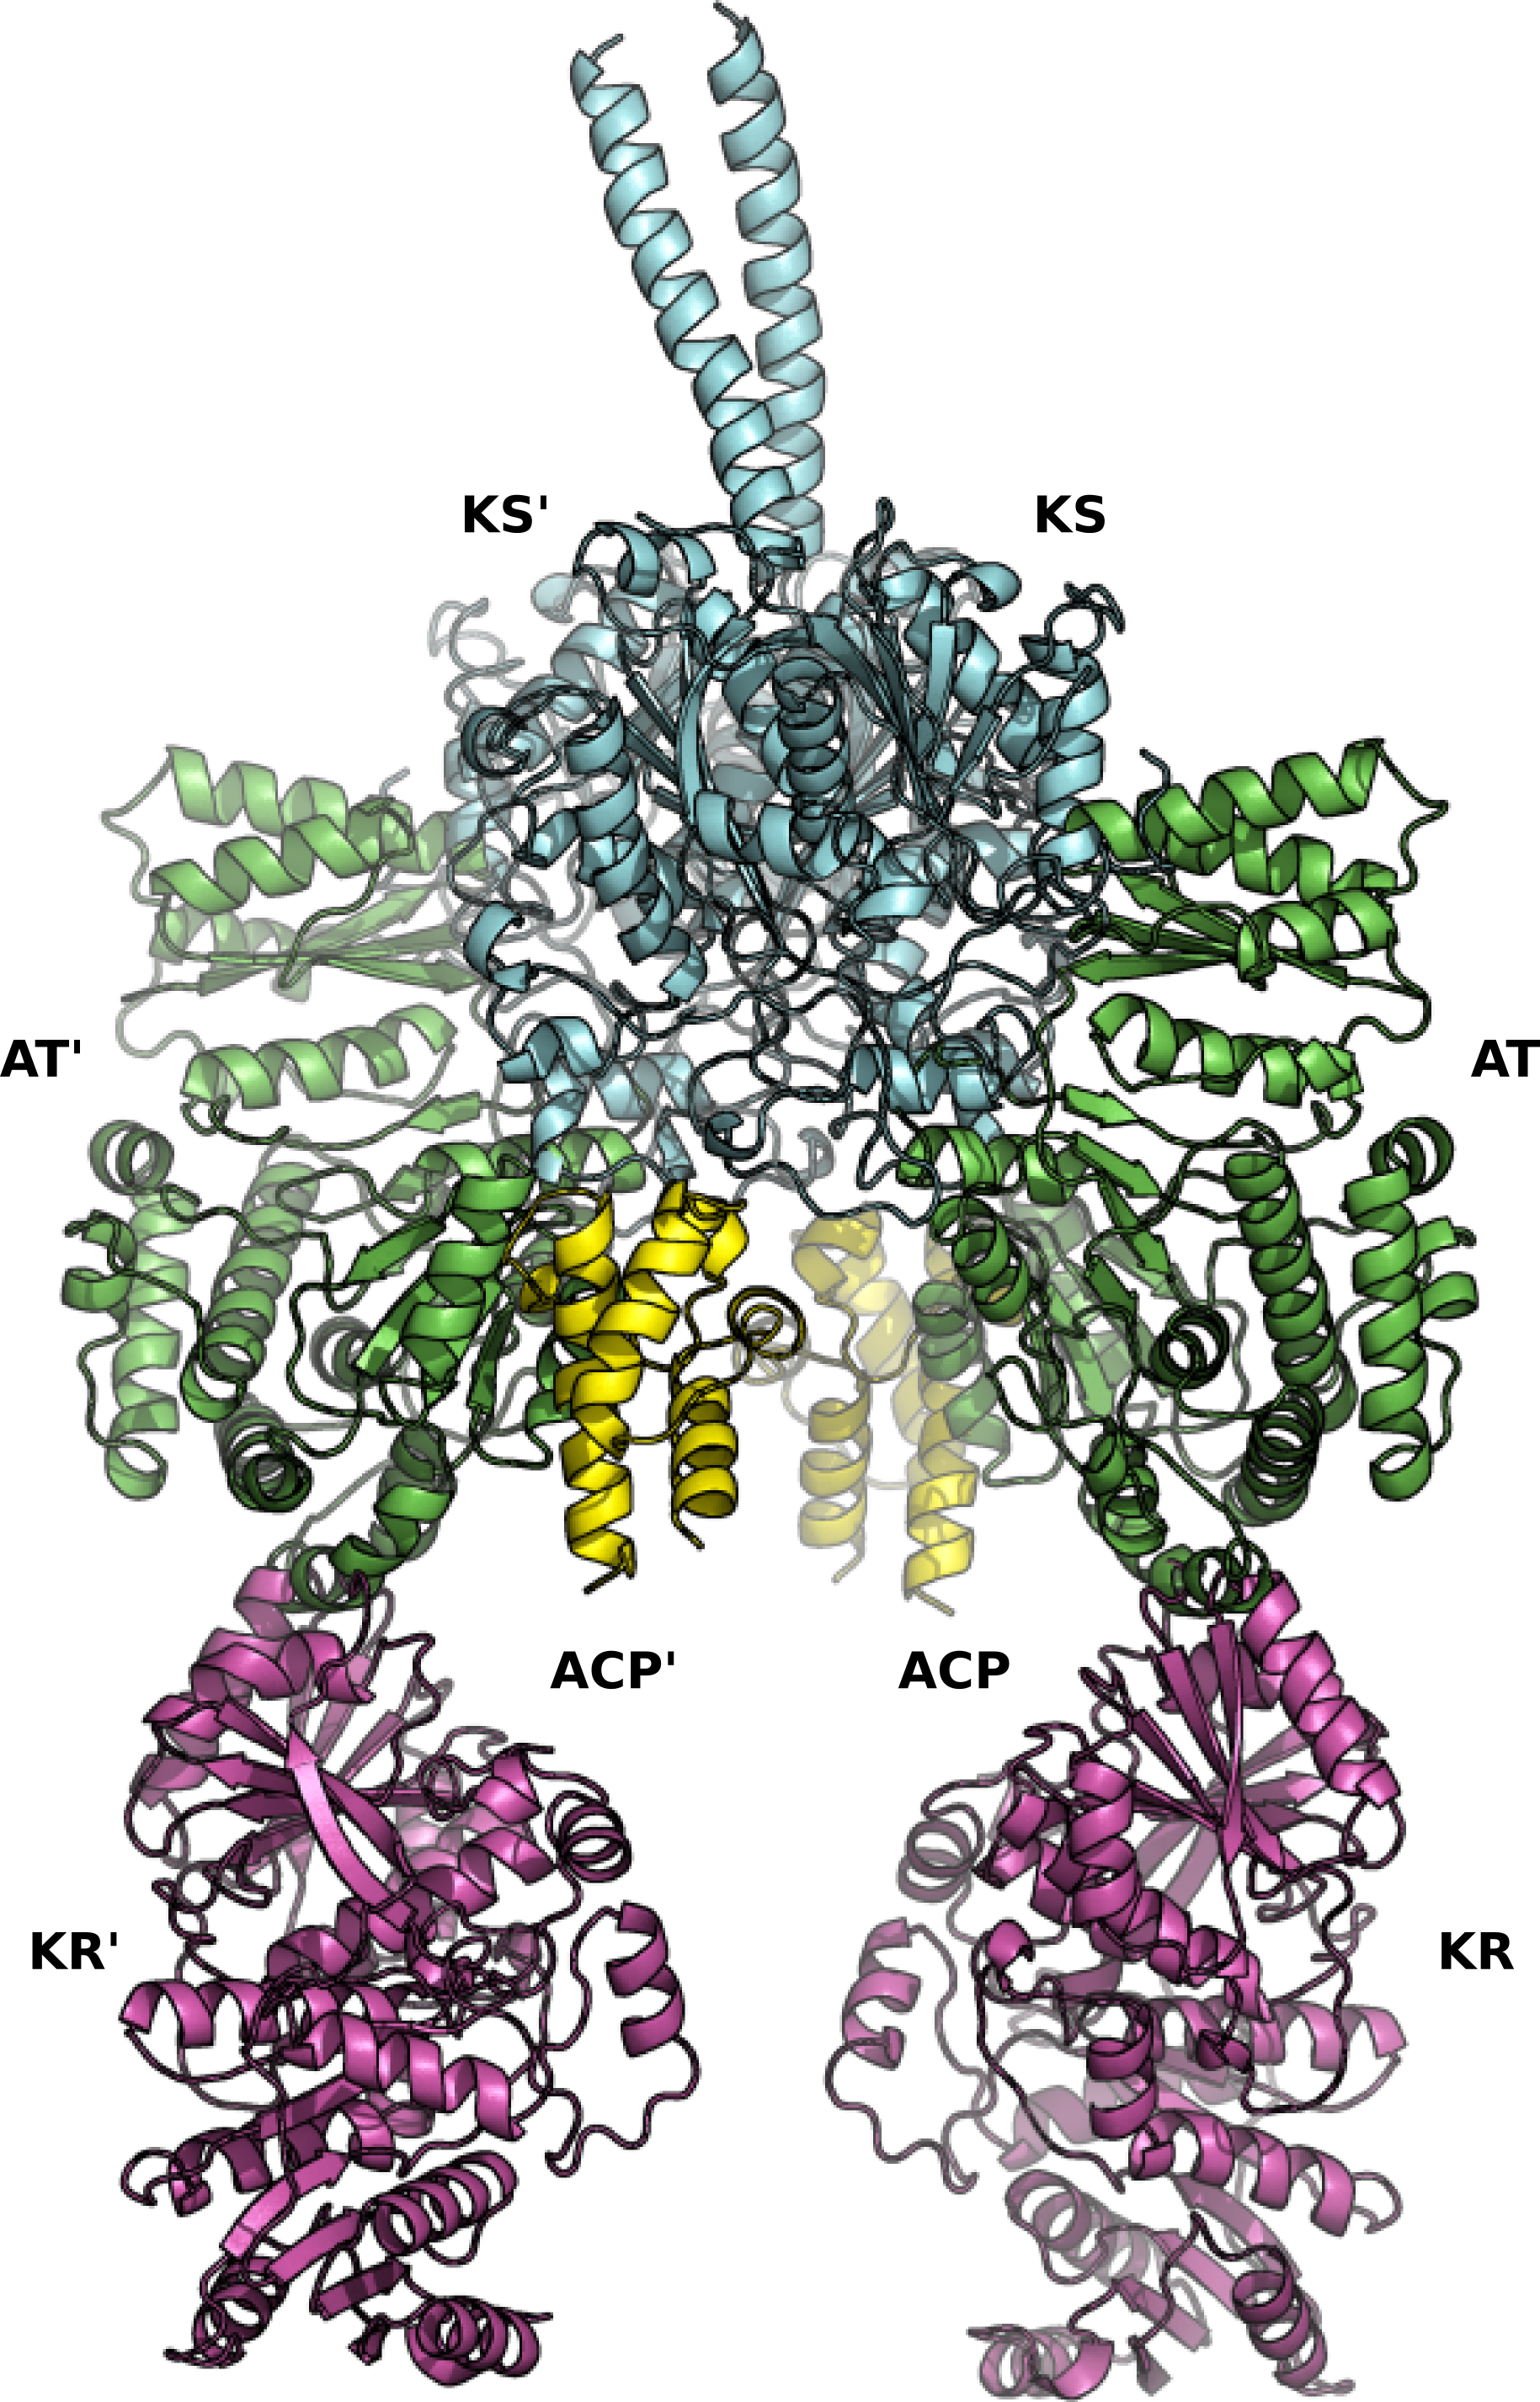
\includegraphics[width=0.80\textwidth, resolution=600, keepaspectratio=true]{graphics/emPksStructure.png}}
			\caption[EM structure of module 5 (PikAIII) from pikromycin cluster]{EM structure of module 5 (PikAIII) from pikromycin cluster. Ketosynthase (KS) dimers are coloured in cyan, acyl transferase (AT) domains are coloured in green, ketoreductase (KR) domains are coloured in magenta and acyl carrier protein (ACP) domains are coloured in yellow \parencite{Dutta2014}.}
			\label{fig:emPksStructure}
			\end{figure}					
					
		The EM structure revealed a striking difference between the PikAIII PKS module and the mammalian FAS structure which was till now considered to be the scaffold for the PKS modules as well. The PikAIII structure revealed a single reaction chamber utilized by that module's ACP to reach all the catalytic domains within the module, whereas the ACP from the previous module delivers the polyketide intermediated through a separate entrance outside the reaction chamber. The PikAIII symmetrical dimer folds into an arch shaped structure with KSs forming the dimer interface at the dome with the ATs hanging on either side of the KS dimer rotated at $ \approx $120\textdegree from their relative positions in mammalian FAS and also DEBS KS-AT dimer structures. The AT domains were also found to form an extensive interface with the KSs as compared to their counterparts in the mammalian FAS and DEBS KS-AT structures. The KR domains are lowered towards the base of the arch attached to the AT domains with the active sites of the AT and KR domains facing towards the reaction chamber. The ACPs were found either at the top, just below the KSs in between the two ATs, or at the base of the arch sandwiched between the two KRs. No evidence was detected for the two ACPs to be in different positions at the same time for example one near the ATs and the other near the KRs. 
		
		The cryo-EM maps also revealed that the linkers between the KRs and ACPs are long enough to reach both the KSs in the dimer. In another work from the same group, \textcite{Whicher2014} have shown a structural rearrangement of the KS-AT domains upon substrate binding in the PikAIII. In the parent paper,   \textcite{Dutta2014} have also shown that dimer formation of the PikAIII is not completely dependent on KS dimerization but is partly contributed by the post ACP dimerization helices. The presence or absence of the ACP domains was also found to  influence the orientation of the KR domains. In a PikAIII $ \Delta $ ACP5 strain, the KR domains were found to be rotated at $ \approx $165\textdegree about the axis of the arch legs. Upon expressing ACP4 from the previous module into the PikAIII $ \Delta $ ACP5 strain the ACP4 was found to be interacting at the N-terminal docking domain of the module 5 KSs, completely away from the reaction chamber where ACP5 would be found. This evidence established the involvement of a separate entrance for the acyl chain transfer on the KSs from an upstream module than utilizing the same reaction chamber involved in the chain elongation and \bet-carbon processing. In another unexpected observation KSs were found to have a second entrance to the active site for the entry of the extender units during elongation reaction. This second entrance was previously not reported either in the FAS or PKS structures. 
		
		\subsection{An example of re-engineering PKSs}
		\label{sec: reengineer}
		A number of groups have made contributions to our current understanding of PKS pathways and how to re-engineer them \parencite{Weissman2005, Challis2008, Piel2010, Kwon2012}, with the macrolide systems being particularly popular systems for study \parencite{Park2010}. Much work has been focused on the type I PKSs. For example, Khosla's group have extensively manipulated and modelled the DEBS system \parencite{Khosla2007}. In their work using a number of chimeric constructs of ACPs, crystal structure determination and computational protein-protein docking revealed how an ACP has specificity for the chain elongation in the DEBS pathway \parencite{Kapur2010}. How the same ACP specifically passes the processed substrate onto the next module \parencite{Kapur2010, Kapur2012}, and why a PKS dimer might be required for function.
		
		Chimeras of ACP3 and ACP6 from deoxyerythronolide B synthase, the ACPs from modules 3 and 6 of the synthetic pathway, indicate that the loop between helix I and helix II were critical during the elongation process of synthesis. Computer docking of the ACP onto the crystal structure of the KS5-AT5 homodimer indicated two residues in the loop that appeared critical for electrostatic complementarity (D44 and R45). Further modelling showed electrostatic complementarity between the KS-AT didomain in each module and the equivalent residues in their cognate ACP, ACP3 (R44, R45), ACP4 (R44, K45), ACP5 (D44, R45) and ACP6 (D44, Q45). Mutations R44A/R45A in ACP3 confirmed the importance of the residues at these positions. The authors noted that these key residues of the ACP interact with the linker (docking domain) between the KS and AT modules, as well as the AT module, and thus this mechanism cannot be the same for PKSs that have the AT acting in trans unless it docks in a similar orientation to the cis AT.
		
		In contrast to the elongation mechanism, for the transfer of the substrate from an ACP to the KS on the next module they found a different mechanism, one that relied on the $ 1^{st} $ ten residues in helix I of the ACP. They also concluded that the PKS domains are made up of subdomains and they have a distinct role in mediating interdomain interaction. These experiments also support the idea of homodimeric architecture of multimodular PKSs. This work emphasizes the benefit of computational modelling working together with well-designed experiments to elucidate the engineering principles underlying the PKS.
		
		From understanding the principle behind the ACP-KS recognition in the polyketide chain elongation and translocation steps, an obvious question arises. Is there a way that this unidirectional ratchet flow of the pathway can be modified? Khosla's group identified a charge complementarity mechanism during chain elongation at the position 23 on the ACP at the KS-AT interaction interface. They found that the opposite charge on KS-AT linker of the following module attracts the preceding ACP, whereas the similar charge on the KS-AT linker of the parent module repels it, thus allowing the reaction to always move forward. Exploiting this mechanism they re-programmed module 3 of the DEBs system to carry out an iterative step of chain elongation. In an experiment they swapped the helix I of ACP3 with the helix I of ACP2, as the helix I is responsible for the chain elongation step. This swapping did not allow the ACP3 to transfer the chain to the module 4 instead it falls back to the KS3 in the module 3 for one more round of chain elongation. The reaction stopped after one round of iterative chain elongation for reasons unknown. However, it could be a limitation of the KS active site to accommodate the larger substrate.
		
	\section{NRPS}
	\label{sec:NRPS}
	Nonribosomal peptide syntetases (NRPSs) are also highly prevalent in secondary metabolite biosynthesis and often synthesize compounds in conjunction with PKSs. The NRPS and PKS systems have similar modular structures and thus NRPSs warrant some discussion here. Nonribosomal peptides are the product of the sequential addition of amino acid monomers catalyzed by NRPSs, involving the domains similar in function to that of PKS system. The amino acid monomers are selected and activated by an adenylation (A) domain which transfers to a thiolation domain or a peptide carrier protein (T or PCP), peptide bond formation is catalyzed by a condensation (C) domain. The PCP has a phosphopantetheine prosthetic group that facilitates the transfer of growing peptide chain/monomers to the various active sites and function analogously to an ACP with a similar four helix bundle structure. The adenylation (A) domain, condensation (C) domain and thiolation or peptide carrier protein (PCP) form the minimal set of domains required to carry out the NRP biosynthesis. In both, the modular PKS and NRPS system the individual domains are linked together by a polypeptide linker region which has also been found to be responsible for functional communication within the domains.
	
	\section{Mupirocin}
	\label{sec:Mup}
	Mupirocin is a polyketide antibiotic used as a topical drug against MRSA and various other  Gram positive bacteria, to treat bacterial skin and hospital acquired infections \parencite{Fuller1971}. Mupirocin is produced by \textit{Pseudomonas fluorescens} NCIMB 10586 and consists of four different pseudomonic acids (PAs) A,B,C and D. PA A, B, C, D contributes 90\%, 8\%, \textless2\% and \textless2\% respectively to the mixture. PAs are made up of monic acid esterified to 9-hydroxynonanoic acid (Figure \ref{fig:mupirocin}). Mupirocin acts by inhibiting bacterial isoleucine tRNA synthetase \nomenclature{IleRS}{Isoleucine tRNA synthetase} thus inhibiting protein production resulting in the cell death \parencite{Hughes1978}.
	
	\setlength\fboxsep{5pt}
	\setlength\fboxrule{1.5pt}
	\begin{figure} []
	\centering
	\fbox{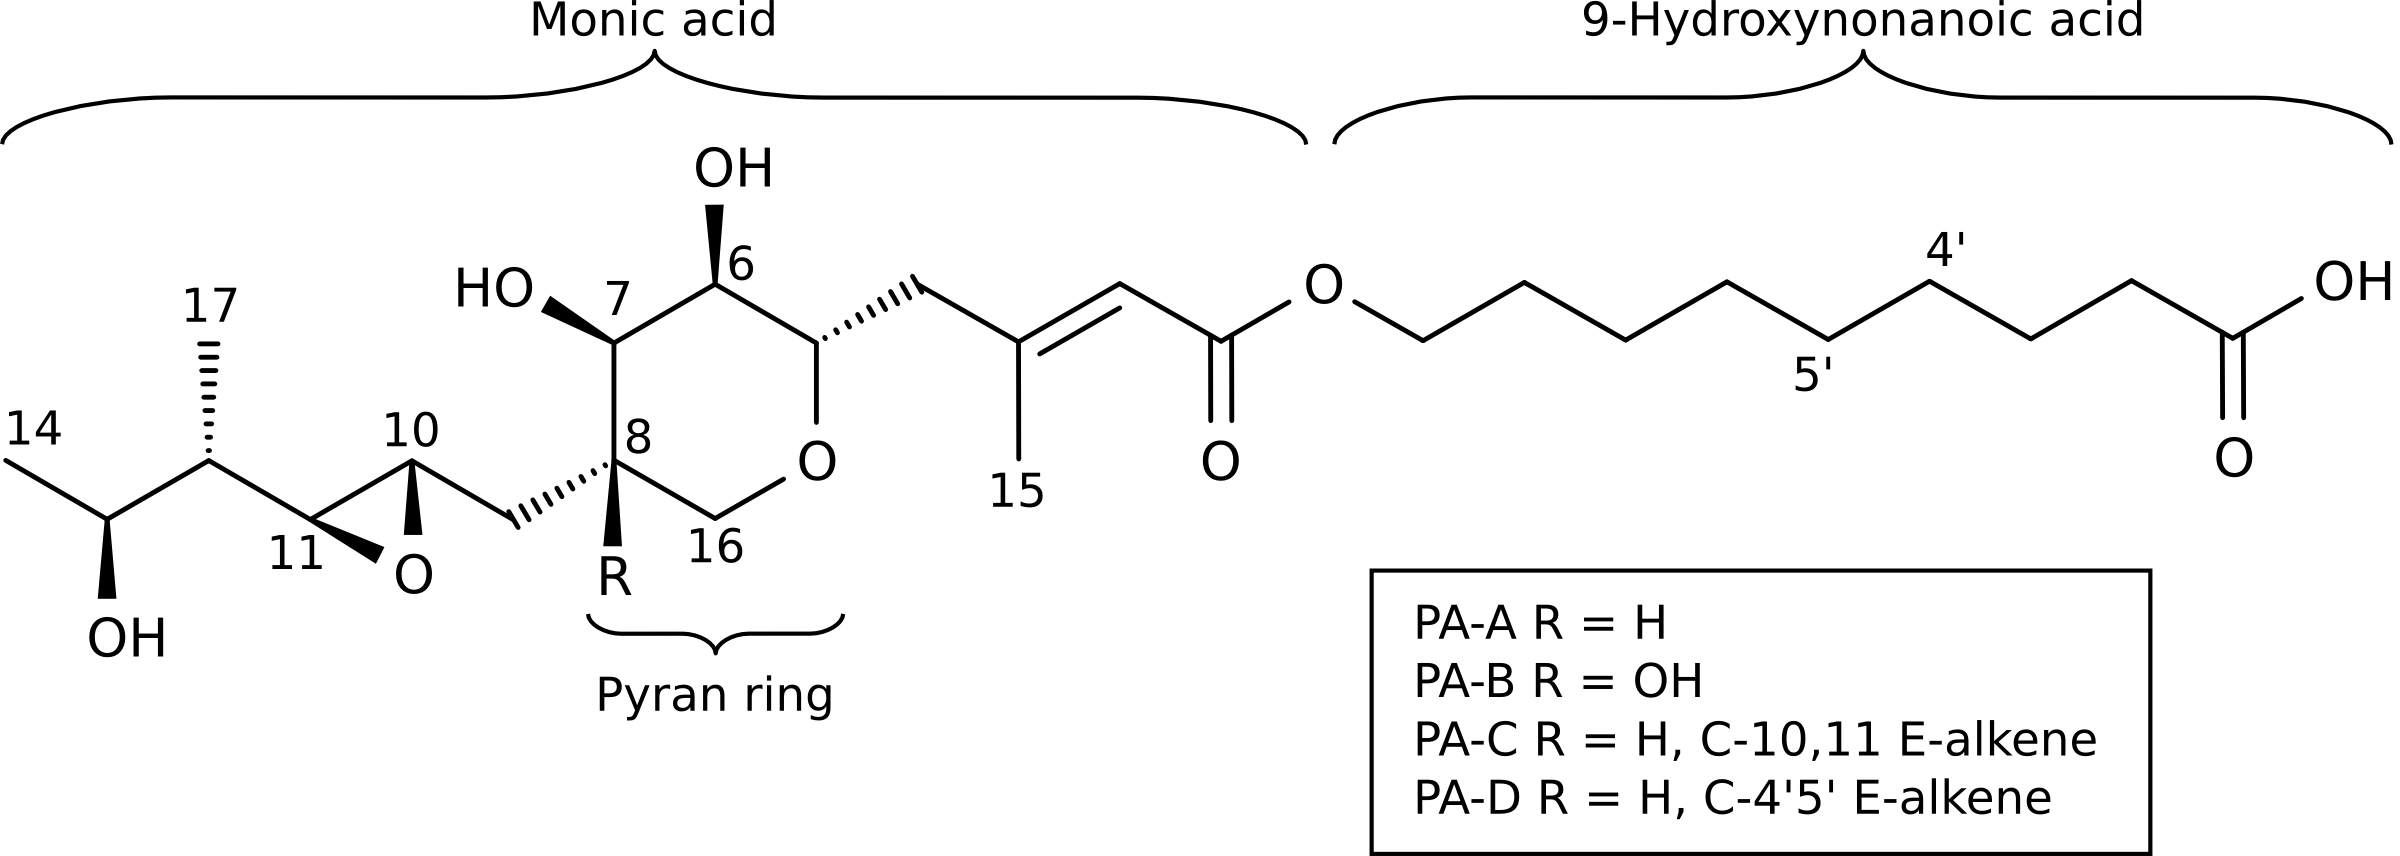
\includegraphics[width=0.8\textwidth, resolution=600, keepaspectratio=true]{graphics/mupirocin.png}}
	\caption[Mupirocin structure]{Mupirocin structure}
	\label{fig:mupirocin}
	\end{figure}
	
		\subsection{Mupirocin Drawbacks}
		\label{sec:MupDrawbacks}
		Mupirocin has proved to be more potent on bacterial IleRS than on the corresponding eukaryotic enzyme, which is highly desirable for any pharmaceutical product. Weak affinity for the eukaryotic IleRS minimises the chances of eukaryotic toxicity and side effects of the drug. Thus, the pseudomonic acids have excellent structures and biological activity as pharmaceutical compounds. However, mupirocin can only be used as a tropical drug as it gets disintegrated inside the body by the hydrolysis of the ester bond between monic and 9-hydoxynonanoic acid (Figure \ref{fig:mupirocin}). It also loses its activity at higher pH, thus preventing it from being used as a systemic drug.
		
		Recent studies \parencite{Patel2009, Thomas2010} have also shown increasing occurrences of mupirocin resistance in \textit{S. aureus}. This resistance can be of low level as well as high level. In low level Mupirocin resistance a single amino acid mutation has been observed in the Rossmann fold region of IleRS, which normally binds to the ATP or else to the 9-hydroxynonanoic acid of Mupirocin. Hence the single amino acid change prevents Mupirocin from inhibiting its target. High level resistance usually results from the presence of eukaryotic like IleRS. This can be acquired either through horizontal gene transfer or through a plasmid containing the mupA gene. The \textit{P. fluorescens} strain, which produces mupirocin, has two different IleRS producing genes of which one is similar to eukaryotic IleRS. This eukaryotic similar IleRS enables \textit{P. fluorescens} to keep on synthesising proteins even at high concentration of Mupirocin. Low-level resistance is not of present concern but the high-level resistance in clinical strains of \textit{S. aureus} acquired through the expression of the mupA gene is alarming. Many of the plasmids containing these genes can conjugate which may cause clonal expansion of the resistant strains.
		
		Therefore with increasing levels of Mupirocin resistance and its limitation for systemic use, there is a need to develop new analogues which may overcome the limitations of Mupirocin. However, before we reach up to the level of producing new analogues we need to understand better the underlying pathway.
		
		\subsection{Mupirocin Biosynthesis}
		\label{sec:MupBiosynthesis}
		The mupirocin biosynthetic cluster (\textit{mup}) consists of a 75kb region encoding 35 ORFs. Figure 1.5 explains the mup cluster and the probable pathway as proposed by Thomas and co- workers \parencite{Thomas2010, Gurney2011}. The \textit{mup} cluster encodes six designated MMPs (Mupirocin multifunctional proteins; \textit{mmpA} to \textit{mmpF}) out of which five encode for polyketide synthases. The non-PKS domain is MmpC, encoding two acyltransferase domains, which is a characteristic of a trans AT system. The proposed biosynthesic pathway initiates in a typical Type I PKS manner where MmpD holds the first starter unit and produces a C$ _{12} $ unit, with MmpA extending this to  C$_{17} $, with further tailoring enzymes producing monic acid. MmpD and MmpA consist of four and three modules respectively each containing a KS and ACP domain. MmpD also consists of KR, DH and MT domains while MmpA only has one KR domain. The first module in MmpD has a non-functional DH and the first module in MmpA is proposed to be involved with the transfer of the growing polyketide chain from MmpD to MmpA. Mupirocin biosynthesis starts with an activated acetyl as a starter unit and uses malonyl-CoA as an extender unit. C$_{16} $ and  C$_{17} $ carbons in the monic acid unit are derived from S-adenosyl methionine (SAM).

		\setlength\fboxsep{5pt}
		\setlength\fboxrule{1.5pt}
		\begin{sidewaysfigure} []
		\centering
		\fbox{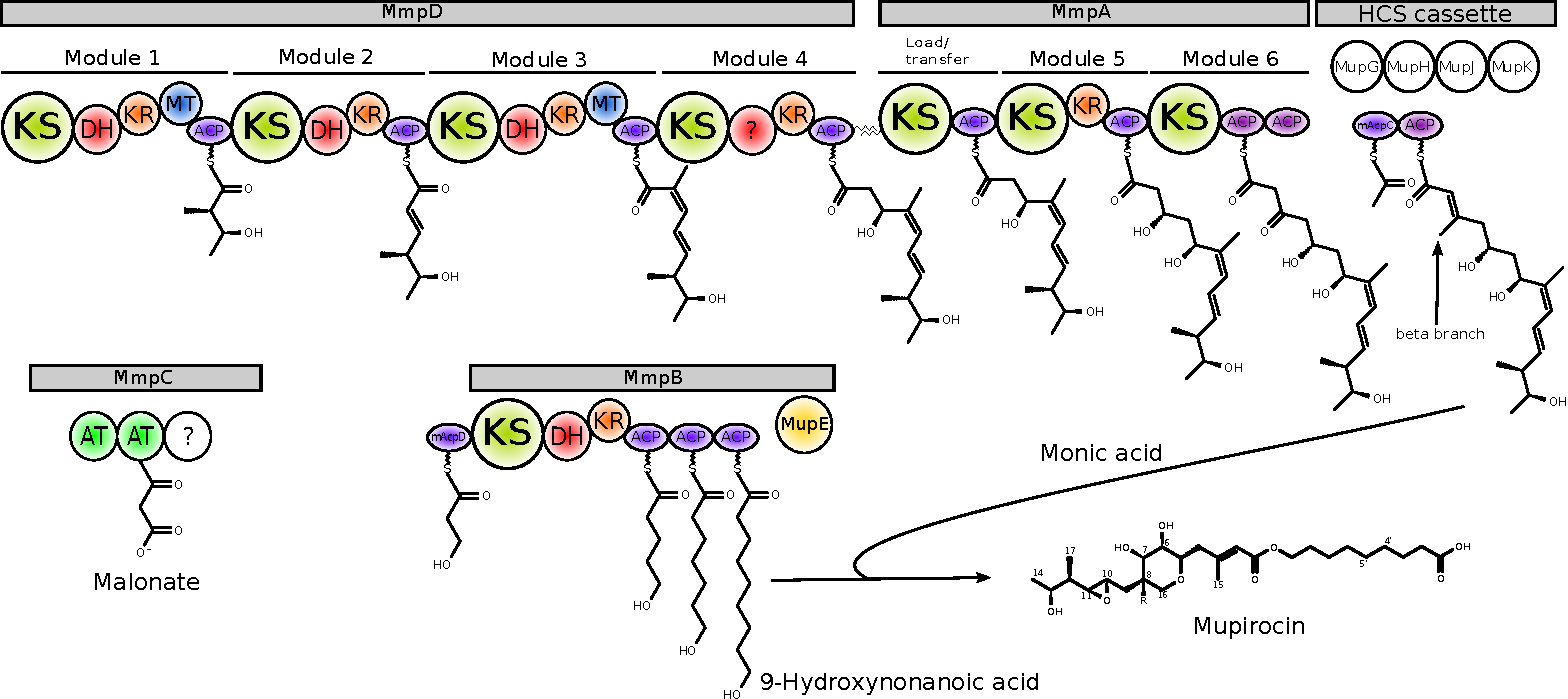
\includegraphics[width=\textwidth, resolution=600, keepaspectratio=true]{graphics/muppathway.pdf}}
		\caption[Mupirocin biosynthesis pathway]{Mupirocin biosynthesis pathway. Figure adapted from \parencite{Thomas2010}.}
		\label{fig:muppathway}
		\end{sidewaysfigure}
					
		The C$_{15} $ carbon is hypothesised to be incorporated by the HMG-CoA synthases activity of MupH in the HCS cassette (MupG, MupH, MupJ and MupK). Knocking out any of the HCS genes stalls the pathway at the end of MmpA and results in the accumulation of intermediate mupirocin H. \parencite{Wu2007}. The HCS cassette has at least four enzymatic functions: an ACP, a hydroxymethyl glutaryl-CoA synthase, a decarboxylase and one or more dehydratases from the crotonase superfamily, in some cases supplemented with other functions. HCS cassettes variously introduce e.g. \bet-methyl, cyclopropane and vinyl chloride moieties, depending on the system they are found in and the exact nature of the cassette. HCS cassettes are found to act on the type I modules, which lack KR, DH or ER domains but which  tend to have tandemly repeated ACPs. Given the variety of functions that the HCS cassette can perform, artificially including them in a PKS cluster provides a powerful tool for the synthesis of novel compounds. To achieve this we need to understand what allows the enzymes of the cassette to know at what point in the pathway they are supposed to work, in particular how a system such as myxovirescin uses two HCS cassettes to produce two specific $ \beta $ modifications in the same system.
		
		\textit{MupC, mupF, mupO, mupU, mupV} and \textit{macp}E provides the correct oxidation state around the pyran ring and mutating any of these genes would result in the accumulation of pseudomonic acid B. Whereas MupT and MupW are hypothesised to be involved in the activation of methyl group C$_{8} $  in order to create the pyran ring.
		
		Finally, MmpB is proposed to synthesise 9-hydroxynonanoic acid starting from 3-hydroxy-propionate via three condensations with malonate iterated three times in the same PKS.  3-hydroxypropionate starter unit is hypothesized to be produced jointly by mAcpD, MupS and MupQ. It is also not understood whether 3-hydroxy-propionate is first attached to mAcpD and then elongated to produce 9-hydroxynonanoic acid or is first esterified to monic acid and then elongated further.
		
		The mupirocin biosynthesis pathway has an ACP doublet (ACPmupA3a/b in MmpA) and an ACP triplet (ACP5, 6 and 7 in MmpB) which is thought to hold multiple substrates for high throughput in rate limiting steps. Apart from the six orfs, which code for the Mmps, the rest of the orfs encode for discrete polypeptides.
		
	\section{Bioinformatics approaches in PKS research}
	\label{sec:BioinfoPKS}
	Research into PKS pathways has been carried out in two major areas. Firstly to identify and experimentally characterize new polyketide natural products and secondly, to develop a synthetic biology tool box for the design and synthesis of novel “natural” products by the re-engineering of naturally occurring polyketide biosynthetic machinery, both of which might provide the basis for novel drugs. Bioinformatics analysis of PKS clusters has played a major role in guiding recent experiments via a variety of tools, examples are PKSDB \parencite{Yadav2003} a database of PKS domains developed a decade ago, which was one of the first tools available, SBSPKS \parencite{Anand2010} and antiSMASH \parencite{Medema2011}, which are recent advanced sequence analysis tools guided by protein structure analysis.
	
	Most work in the field has focused on the core PKS functions, particularly type I PKSs, thus there is still little known about the mechanisms of the tailoring enzymes acting in trans. Such tailoring enzymes are an essential part of any PKS system since they provide additional chemical diversity to the polyketide chain. An ability to predict the function of tailoring enzymes and their compatibility with other PKS modules would provide much additional functionality to the synthetic biology tool box. \textit{Trans}-AT systems are less well studied and since software tools are primarily targeted at \textit{cis}-AT systems they tend to completely fail or have limited capabilities in predicting \textit{trans}-AT systems.
%	
	PKSDB/SEARCHPKS and NRPS-PKS were the first available webservers for identifying PKS/NRPS domains in an unknown sequence as well as relating PKS/NRPS sequences to their corresponding secondary metabolites; recent reviews \parencite{Jenke-Kodama2009, Bachmann2009} give a detailed discussion on the utility of the PKSDB and the NRPS-PKS databases. Following similar lines, resources like ASMPKS \parencite{Tae2007}, ClustScan \parencite{Starcevic2008}, CLUSEAN \parencite{Weber2009}, NP.searcher \parencite{Li2009}, NRPSpredictor \parencite{Rottig2011}, NRPSsp \parencite{Prieto2012} and antiSMASH \parencite{Medema2011} have been developed for the discovery of secondary metabolites through genome analysis. All these servers primarily utilize sequence information either for domain identification or to correlate the various PKS domains to their corresponding metabolic products. However, many of them also utilize structural information for predicting the most likely starter and extender units picked by the acyl transferase domains, and SBSPKS models the 3D structure of PKS modules. Table  \ref{tab:pks_res} gives a summary of the resources available for PKS/NRPS pathway analysis with a detailed description in Section \ref{sec:comptools} of Appendix IV.
%		
\newpage		
		\begin{singlespace}
		\begin{small}
		\begin{longtabu}[tbp]{p{2.5cm} p{2cm} p{2cm} p{2cm} p{2cm} p{2.5cm}}
		\caption{Resources available for secondary metabolite prediction.}
		\\ \hline\hline\hline
		 \bf{Resources} & \bf{Clusters/ types} & \bf{Prediction tools} & \bf{Domain for which specifity is predicted} & \bf{Backend or Training data source} & \bf{Hyperlink} \\ \hline\hline\hline
		SEARCHPKS, PKSDB (database) & PKS & BLAST & AT & PKSDB & \url{http://www.nii.res.in/searchpks.html} \\ \hline
		NRPS-PKS (database) & NRPS, PKS & BLAST & AT, A	& PKSDB, NRPSDB, ITERDB, CHSDB & \url{http://www.nii.res.in/nrps-pks.html} \\ \hline
		ASMPKS & PKS & GLIMMER, BLAST & AT & PKSDB, More & \url{http://gate.smallsoft.co.kr:8008/~hstae/asmpks/genome.pl} \\ \hline 
		NRPSpredictor, NRPSpredictor2 & NRPS & SVM, TSVM & A & Training data amalgamated from various sources &	\url{http://nrps.informatik.uni-tuebingen.de/Controller?cmd=SubmitJob} \\ \hline 
		CLUSTSCAN, CompGen (homologous recombination module) & PKS, NRPS, PKS-NRPS hybrid & HMM	& KR, AT & Pfam, Specialized & \url{http://bioserv.pbf.hr/cms/}, \url{http://bioserv.pbf.hr/cms/index.php?page=compgen} \\ \hline
		SBSPKS & NRPS, PKS & BLAST, 3D structure modelling & AT, A & PKSDB, NRPSDB, ITERDB, CHSDB & \url{http://www.nii.ac.in/~pksdb/sbspks/master.html} \\ \hline
		NORINE (database) & NRPS products, monomers & & & & \url{http://bioinfo.lifl.fr/norine/} \\ \hline
		CLUSEAN (Perl module framework)	& NRPS, PKS & BLAST, HMM & A & NCBI NR, Pfam, Specialized & \url{http://redmine.secondarymetabolites.org/projects/clusean} \\ \hline
		antiSMASH (metaserver \& standalone) & NRPS, PKS, terpenes, aminoglycosides, amino-coumarins, indolocarbazoles, lantibiotics, bacteriocins, nucleosides, β-lactams, butyrolactones, siderophores, melanins and others & NCBI BLAST+, HMMer, Muscle, Glimmer, FastTree, TreeGraph & AT, A, KR & Amalgamated from various previously published works	& \url{http://antismash.secondarymetabolites.org/} \\ \hline\hline\hline
		\label{tab:pks_res}
		\end{longtabu}
		\end{small}
		\end{singlespace}

	\section{Research objectives and thesis outline}
	\label{sec:researchobjectives}
	The mupirocin biosynthesis pathway provides a model system for understanding \textit{trans}-AT PKSs, and contributing to our understanding of the way proteins and substrate recognition events are regulated. In the present work the analysis was mainly focused on the structural modelling of the protein complexes involved in the mupirocin synthesis via the tools of structural bioinformatics supplemented with information from experiments. The findings in this thesis will be a prototype for the modelling of large macromolecular complexes in prokaryotic systems and the structural models produced will enhance our understanding of the synthetic pathways allowing us to re-engineer them with greater success. 
	
	The overall thesis is divided into four results chapters Chapter 3 to 6, which discuss the results of three major projects in their respective chapters and two minor projects compiled in one chapter. Chapter 2 describes the methods used in the different projects in detail. The last chapter of the thesis summarizes and discusses the entire thesis. 
	
	The project discussed in Chapter 3, aimed to elucidate the mode of interaction between ACP-mupA3ab:MupH complex, which are involved in beta branching, proposing key interacting residues for mutagenesis experiments. Structural models and properties of MupH the HMG-CoA synthase homologue in HCS cassette were predicted using various bioinformatics tools. ACP sequences from characterised PKS pathways were also classified into beta and non-beta branching type using hidden Markov model analysis. Mutagenesis experiments carried out by Prof. Thomas' group on the predicted ACP:MupH interface supports the predicted complex and residues responsible for the specificity of the interaction. Some of the findings of this project are already published in \textcite{Haines2013}.
	
	Based on the hypothesis generated in the first project, further lab experiments were carried out as described in Chapter 4. The aim was to complement the \bet-branching-ACPs in the mupirocin cluster with the \bet-branching-ACP(s) from the kalimantacin cluster. It was hypothesized that the \bet-branching ACP(s) from the kalimantacin cluster would not work with MupH but will work with BatC (MupH equivalent form kalimantacin cluster). The aim was also to identify the key residues at the interface of the \bet-branching ACPs from the \textit{mup} cluster and BatC which can be modified to work efficiently with BatC.
	
	As the experiments and molecular dynamics (MD) simulations carried out on FAS ACPs \parencite{Chan2008} have shown the formation of a hydrophobic tunnel which sequesters the fatty acid chain, the third project was to see if a similar mechanism might exist in the PKS ACPs. Molecular dynamics simulations of the ACPs from module 2 and 3 of MmpA in the mupirocin cluster were carried out in explicit solvent with a time scale of 50 ns to 1 $ \mu $s. Several macroscopic properties were calculated by analysing the MD simulation trajectories, a sequestering of the substrate to the ACP surface was seen but the atomic details are different from what was seen in the FAS system. 
	
	Chapter 6 presents the results of two independent projects, the first project aimed to find out the means of recognition specificity of the KS-mupA2 towards the predicted $ \alpha $-OH substituted substrate and the results suggest a specific recognition motif that may stall substrate progression until it has been hydroxylated. The second project aimed to investigate the significance of movements of loops on the MupH surface that were seen in the simulations presented in Chapter 4. Simulations suggested the loops may leave easy access to the active site until the substrate is bound.
	

	

\nomenclature{Mup}{Mupirocin cluster}
\nomenclature{Mmp}{Mupirocin multi functional proteins}
\nomenclature{MD}{Molecular dynamics}
\nomenclature{6-MSA}{6-methyl-salicylic acid}
\nomenclature{HCS}{3-hydroxy-3-methyl glutryl-CoA synthase cassette}
\nomenclature{HMG-CoA}{3-hydroxy-3-methyl glutryl-CoA}
\nomenclature{MS}{Mass spectrometry}
\nomenclature{bp}{Basepair}
\nomenclature{DEBS}{6-deoxyerythronolide B synthase}
\nomenclature{MAT}{Malonyl transferase}
\nomenclature{MT}{Methyl transferase}
\nomenclature{SNAC}{Sodium 8-((2-hydroxybenzoyl)amino)octanoate}
\nomenclature{SDR}{Short chain dehydrogenases/reductases}
\nomenclature{NADPH}{Nicotinamide adenine dinucleotide phosphate}
\nomenclature{MDR}{Medium chain dehydrogenase reductases}
\nomenclature{PPT}{Phosphopantetheinyl transferase}
\nomenclature{MRSA}{Methicillin-resistant \textit{S. aureus}}
\nomenclature{INSDC}{International Nucleotide Sequence Database Collaboration}
\nomenclature{CDS}{coding sequences}
\nomenclature{PSI-BLAST}{Position Specific Iterative - Basic Local Alignment Search Tool}
\nomenclature{PSSM}{Position specific scoring matrix}
\nomenclature{PHI-BLAST}{Pattern Hit Initiated - Basic Local Alignment Search Tool}
\nomenclature{HMM}{Hidden Markov model}
\nomenclature{SASA}{solvent accessible surface area}
\nomenclature{EDTA}{Ethylenediaminetetraacetic acid}
\nomenclature{TAE}{Tris Acetate EDTA}
\nomenclature{TTC}{Triphenyl tetrazolium chloride}
\nomenclature{AIR}{Ambiguous interaction restraints}
\nomenclature{MSA}{Multiple sequence alignment}
	\chapter{Materials and Methods}
\label{cha:MaterialsAndMethods}

	\section{Databases}
	\label{sec:Databases}
	In the present study various databases have been used to retrieve sequence (DNA and Protein) and protein structure information. For the sequence analysis in Section \ref{sec: ACPSequenceAnalysis} RefSeq microbial and UniProtKB/TrEMBL (with 6408654 seq and 20127441 seq respectively, as on 9$^{th}$ March, 2012) were used to search for ACP homologues using the hidden Markov models. RefSeq is a non-redundant database of DNA, RNA and protein sequences curated by the sequences from International Nucleotide Sequence Database Collaboration (INSDC) hosted at the National Centre for Biotechnology Information (NCBI) \nomenclature{NCBI}{National Centre for Biotechnology Information}. RefSeq (\url{http://www.ncbi.nlm.nih.gov/refseq/}) provides the reference sequence for a species, each entry being annotated and cross-linked to other databases by collaborating groups and NCBI staff. RefSeq can be accessed via the Entrez search engine, through a sequence similarity search using BLAST \nomenclature{BLAST}{Basic Local Alignment Search Tool} or by the RefSeq FTP server. The RefSeq microbial dataset was used, which consists of sequences from microbial genomes/proteomes. 

	UniProtKB/TrEMBL (\url{http://www.uniprot.org}) is a collection of computationally annotated protein sequences. The sequences in UniProtKB/TrEMBL are derived from the computational translation of the coding sequences (CDS) submitted in INSDC databases. UniProtKB/TrEMBL can be accessed through keyword or uniprot identifier searches on the UniProtKB website or through a sequence similarity search using BLAST. The purpose of selecting two databases was not only to retrieve the highest quality sequence information from a curated database but also to have maximum coverage of sequences available through an automated database. The sequence data from both the databases were obtained from their FTP websites in the FASTA format.
	
	For molecular modelling, as explained in Section \ref{sec:HomologyModelling}, protein structure coordinate information was taken from the Protein Data Bank (PDB) \nomenclature{PDB}{Protein Data Bank} (\url{http://www.rcsb.org}). The PDB is the single archive for macromolecule (DNA and Protein) 3D coordinate information. It consists of structural information determined through experimental methods such as NMR spectroscopy and X-ray crystallography. The PDB database can be searched by keyword or PDB identifier, or by running a BLAST similarity search either from within the PDB website or through NCBI BLAST.
	
	\section{Sequence analysis}
	\label{sec:SequenceAnalysis}
	In molecular biology, routine sequence analysis is carried out to infer the biological function of newly sequenced DNA or protein sequences. For the purpose of inferring biological function similarity searches against annotated sequence databases using pairwise alignment methods such as BLAST and FASTA are in common use. Pairwise sequence alignment methods give equal weighting to all aligned positions. However, in a multiple sequence alignment it can be clearly seen that several positions within a family of proteins are under more evolutionary pressure to be conserved than others. Thus pairwise sequence alignment methods are good for fast searches of closely related sequences but are poor at detecting remote homology. In contrast, methods based on position specific scoring and probability such as Profiles and hidden Markov models are much more sensitive in detecting remote homology. 
		
		\subsection{PSI-BLAST and multiple sequence alignment}
		\label{sec:PSIBlastAndMSA}
		In the present study position specific iterative BLAST (PSI-BLAST) has been used to identify template structures for homology modelling (see Section \ref{sec:HomologyModelling}). PSI-BLAST is an extension of the normal protein-protein BLAST but it uses a position specific scoring matrix (PSSM) or profile. This PSSM is generated from the multiple sequence alignment of the sequences found in a normal protein BLAST, which is the first iteration of PSI-BLAST. The PSSM is used and refined in further iterations of PSI-BLAST, rather than a simple sequence. PSI-BLAST is more sensitive in detecting distantly related sequences as compared to the normal protein-protein BLAST. 
		
		In Section \ref{sec: ACPSequenceAnalysis} multiple sequence alignments (MSAs) were used to identify conserved residues which differentiate branching-ACPs from non-branching-ACPs. An MSA is created with three or more sequences with the aim of identifying regions of sequence homology and conserved positions, which may be used to characterize a protein family. MSAs are also used for phylogenetic reconstructions as differences between sequences, can be used to estimate how recently two proteins from a given family a common ancestor in a family of protein/DNA sequences. As explained in Section \ref{sec:ET} MSAs were also used for evolutionary trace analysis to predict positions under evolutionary pressure within a clade as compared to between the clades. The ClustalW and Muscle programs were used for generating MSAs.
		
		\subsection{Hidden Markov models (HMMs)}
		\label{sec:HMM}
		HMMs are models which represent a probability distribution of the occurrence of residues for each position in a multiple sequence alignment allowing for the residue type to occur through conservation, insertion, deletion, or some combination of the later two with the aim of encapsulating the common features of a protein family that are necessary to recognize other members of the family. HMMs are built on a set of aligned sequences belonging to a family of proteins. Each column in an MSA is considered as a \textquotedblleft state\textquotedblright which \textquotedblleft emits\textquotedblright symbols (residues) according to the emission probabilities. Each state is interconnected to other states called transitions with state transition probabilities. The model produces the sequence of symbols based on the emission and transition probabilities and the probability of a given sequence being produced is the product of all the emission and transition probabilities. The hidden part in a hidden Markov model is the sequence of the states taken to produce the sequence of symbols. It’s only the “emitted” symbols which are visible, not the underlying state. In practice HMMs are generated (or trained) using an MSA. To align a sequence to an HMM model the HMM can be seen as traversing all the possible sequences of states through the model to generate the target sequence. This will assign the probability values to the sequences produced of which the best ones are selected through a dynamic programming based algorithm such as the Viterbi algorithm.
		
		\subsubsection{HMM analysis of \bet-branching and standard ACPs}
		\label{sec:HMMACPs}
		HMMs were used to classify a subclass of acyl carrier proteins (ACPs) called the branching ACPs (for results see Section \ref{sec: ACPSequenceAnalysis}). The two HMM models were built using the HMMER program from the 15 clusters with known pathways, with 38 and 178 sequences (sequences provided by Dr. Anthony Haines) for the branching and the non-branching-ACPs respectively. The training and the test set were scored with each HMM models and the scores were plotted on a scatter graph to highlight two distinct clusters between branching and non-branching ACPs. The non-branching HMM model was also searched against TrEMBL and RefSeq databases which fetched 16,490 unique sequences with the length greater or equal to 60 amino acids. These sequences were also scored with both the models and plotted in a separate scatter plot along with the training set.  The models were deposited with SMART since no domain prediction software (SMART, Pfam etc.) had the capacity to distinguish these two types of ACP.
	
	\section{Molecular Modelling}
	\label{sec:MolecularModelling}
	The present study aims to model the polyketide synthase complexes which are large macromolecular complexes. Determining the structure of large protein complexes through experimental methods such as X-ray crystallography and NMR \nomenclature{NMR}{Nuclear Magnateic Resonance} spectroscopy is possible however at times can be quite difficult and time consuming. On the other hand with the increase in computing capacity and the large amount of molecular biology data available it is increasingly possible and efficient to use computational methods to predict structures based on the existing structural data. Molecular modelling can be used for tasks such as protein structure prediction through homology modelling, understanding protein dynamics through molecular dynamics simulations, protein – protein interaction interface prediction and molecular docking to generate atomic resolution three dimensional protein complex structures. 
	
		\subsection{Homology modelling}
		\label{sec:HomologyModelling}
		Homology modelling or comparative modelling is a computational method to generate three dimensional protein structures of atomic resolution. As the name suggests homology modelling is based on the fact that the proteins which perform similar functions tend to have similar sequences with regions important for the function being conserved. Furthermore, the protein structures of even divergent protein sequences, which share a common ancestry, tend to fold into a similar three-dimensional structure. Thus a protein structure can be used to predict the atomic resolution model of a homologous target sequence \Parencite{Chothial1986}. The theoretical models generated through homology modelling primarily rely on the quality of the sequence alignment between the target sequence and the homologous sequence and the quality of the homologous structure. Over the past few years several state of art computational tools have emerged with increasing level of accuracy, which are continually being monitored by the biannual CASP competitions (\url{http://predictioncenter.org/}).
		
		In the present work, different versions of the Modeller \Parencite{Sali1993} program have been used to carry out the homology modelling for all the predicted structures. Modeller generates the three dimensional models of the target protein sequence by satisfying spatial restraints obtained from the sequence alignment of the target and the homologous protein templates. This method in principle is quite similar to employing the distance geometry approach used in NMR experiments. The spatial restraints extracted from the sequence alignment are expressed as probability density functions (PDFs) which are used to restrain C$\alpha$-C$\alpha$ bond distance, N-O distance, main chain and side chain dihedral angles. Apart from the bond distance restraints derived from the sequence-template alignment, stereochemical restraints are added using a molecular mechanics force field. In the final model building step the model is generated by minimizing the violation of all the restraints \Parencite{Marti-Renom2000, Eswar2006}.
		
		This method of model prediction has an advantage over many other tools for the same purpose as it allows several restraints to be added by the user derived from various resources. It is thus possible to apply restraints derived from experiments such as NMR spectroscopy, fluorescence resonance energy transfer (FRET), crosslinking experiments as well as restraints derived from Bioinformatics based experiments. The model building step can also be coupled with model refinement steps using simulated annealing and molecular dynamics simulations. However, in the present work many of the models were generated without any model refinement step which allows a direct comparison with the template structure as the algorithm places the side chains at the similar positions to the template. %Here Modeller has also been used to model homodimeric proteins for example the ketosynthase homo dimer in MmpA, as found in the X-ray structure of the ketosynthase - acyltransferase didomain of module 5 from DEBS systems (PDB ID 2HG4).
		
			\subsubsection{Modelling of MupH + ligand complex}
			\label{sec:HomologyModellingMupH}
			MupH was modelled using Modeller version 9.8 \Parencite{Eswar2006}. The MupH sequence was used to search the PDB for the solved homologous structures, using PSI-BLAST. 10 structures were selected ranging from 27\% to 32\% sequence identity to generate the initial alignment using ClustalW \Parencite{Larkin2007}. The structures chosen in similarity with the MupH sequence were from the species \textit{Staphylococcus auereus, Enterococcus faecalis, Brassica juncea, Streptococcus mutans} and \textit{Homo sapiens} thus providing a wide range of organisms for comparisons. All the homologues found were HMG-CoA synthases. The secondary structures of the templates, determined by DSSP \Parencite{Joosten2011}, guided manual refinement of the final alignment using Seaview \Parencite{Galtier1996}. The HMG-CoA synthase structure from \textit{Enterococcus faecalis} (PDB ID 1X9E), having 87\% query coverage with 32\% sequence identity, was selected as the template. Modeller produced five structures which were further tested for stereochemical quality using the PROCHECK \Parencite{Laskowski1993} program (\url{http://nihserver.mbi.ucla.edu/SAVES/}). The model with the best PROCHECK score was selected for further analysis. 
			
			In order to dock the polyketide intermediate ligand in the MupH active site the modelled MupH structure was superimposed on the 1X9E crystal structure and the X-ray determined coordinates for the phosphopantetheine moiety from the bound ligand in 1X9E were copied. The rest of the polyketide intermediate was built manually inside the MupH active site using the PyMol program (\url{http://www.pymol.org}). To remove the steric clashes energy minimization was carried out using Chimera \Parencite{Pettersen2004}. The AMBER99SB-ILDN \Parencite{Hornak2006} force field and Antechamber program were used to assign the force field parameters to the protein and ligand respectively. 
			
			\subsubsection{Modelling of ACP-mupA2}
			\label{sec:ACP2modelling}
			ACP-mupA2 (the ACP from the second module of MmpA in the mupirocin cluster) was modelled using Modeller version 9.10. The ACP-mupA2 sequence (GenPept Acc No. AAM12909 range 1822 to 1916) was used to search against the PDB database using BLAST to identify the template. The NMR structure of the Holo-Acpi Domain from the CurA module from \textit{Lyngbya Majuscula} (PDB ID 2LIU) was selected as the best template with 80\% query coverage and 29\% sequence identity. To generate the initial alignment for modelling, a multiple sequence alignment was carried out using two template sequences, 2LIU, 2L22 (ACP-mupA3ab NMR structure from the third module of MmpA in the mupirocin cluster) and other ACP sequences from the mupirocin cluster. Sequence alignment was manually refined using secondary structure information as explained in Section \ref{sec:HomologyModellingMupH} and the homology modelling was carried out using 2LIU as the template, generating five structures. The structures were tested for stereochemical quality using PROCHECK and the structure with the best PROCHECK score was selected for further analysis. 
			
			\subsubsection{Modelling of the KS-mupA2 dimer}
			\label{sec:KS2modelling}
			KS-mupA2 (KS from the second module of MmpA in the mupirocin cluster) was modelled using Modeller version 9.11. KS-mupA2 was modelled as a dimer along with the KS docking domain also called as the linker region between the KS and AT domain in the \textit{cis} systems. KS-mupA2 sequences (GenPept Acc No. AAM12909.2 range 715 to 715 to 1288) was searched against the PDB database using BLAST to identify the template. Two templates from the DEBS system, the KS-AT dimer from module three and five (PDB ID 2QO3 and 2HG4) along with the KS sequences from the mupirocin system, were used to generate the initial alignment which was manually refined using secondary structure information and visual inspection of the alignment. The DEBS structure 2QO3 with 88\% query coverage and 39\% sequence identity was used as the template to generate five homology models. The structures were tested for stereochemical quality using PROCHECK and the structure with the best PROCHECK score was selected for further analysis.
		
		\subsection{Molecular dynamic simulation}
		\label{sec:MolecularDynamicSimulation}
		Molecular dynamic (MD) simulation is a computational method to simulate the time dependent behaviour of a physical system. In molecular modelling, MD simulations of proteins and DNA macromolecules are used to observe the changes in forces and structural dynamics with respect to time. In a typical MD simulation of a physical system of N interacting atoms, such as a protein immersed in a box of solvent, the atoms are allowed to move following Newton's laws of motion. Equation \ref{eq:force} represents the differential form of Newton's second law of motion i.e. F=ma, describing the motion of a particle \textit{i} of mass $ m_{i} $, in the direction $ x_{i} $ with the force $ F_{x_i} $ acting on the particle in the $ x_{i} $ direction. %force F$ _{i} $, on a particle i with coordinates r$ _{i} $, which is equal to the product of mass of the particle m$ _{i} $  and its acceleration. 
		
		\begin{equation}
		\label{eq:force}
			\frac{\delta^2x_i}{\delta t^2} =  \frac{F_{x_i}}{m_i}, i=1 ... N
		\end{equation}
		
%		\noindent Where force is the negative derivative of the potential function $V (r_1, r_2 ... r_N)$.
%		
%		\begin{equation}
%		\label{eq:force1}
%			F_i = - \frac{\delta V}{\delta r_i}
%		\end{equation}
		
		\noindent The calculation of the forces highly depends on the parameters of the molecular mechanics force field equation used. The equation below is the functional form of the AMBER force field equation.
		
		\begin{equation}
		\label{eq:AMBER}
		\begin{gathered}
			V(r^N) = \sum k_b (l-l_0)^2 + \sum k_a (\theta - \theta_0)^2 + \sum \frac{1}{2} V_n [1 + \cos(nw - \gamma)] \\ 
			+ \sum_{j=1}^{N-1} \sum_{i=j+1}^{N} \Biggl \lbrace \Biggl[\epsilon_{ij} \left(  \frac{r_{0ij}}{r_{ij}} \right)^{12} - 2 \left(\frac{r_{0ij}}{r_{ij}}\right)^6 \Biggl] + \frac{q_i q_j}{4 \pi \epsilon_0 r_{ij}} \Biggl\rbrace
		\end{gathered}			
		\end{equation}
		
		The first term in the equation represents the energy of the covalent bonds. The second term represents the energy of the bond angles. The third term represents the energy due to torsional angles and the last term represents the energy due to non-bonded interaction between all the atom pairs, which include van der Waals, and electrostatic energies. 
		
		In molecular dynamics simulation the equation of Newton's second law of motion is solved for the desired length of time. %at the required temperature and pressure. 
		The change in the coordinates of the atoms due to the motion is recorded at regular intervals. The coordinates with respect to time represents the trajectory of the system. Once the system has reached the equilibrium state many macroscopic properties can be studied by averaging over the equilibrium trajectory. MD simulations are widely used in molecular modelling to study folding and unfolding of the proteins, protein structure stability, protein-protein interactions, free energy binding of drug-protein complexes, the effects of mutations on the structural dynamics of the proteins etc. 
		
		In the present study the GROMACS 4 \parencite{Pronk2013} molecular dynamics program has been used to study the protein dynamics in explicit solvent (water) and the protocol can be summarized in three major steps. 
		
		\begin{description}
		\item[Structure preparation] \hfill \\ In the first step, the physical system to be simulated is represented in the computer. The protein structure from X-ray or NMR experiments or through homology modelling contains the coordinate information only. However, for running the MD simulation this coordinate information needs to be expressed in terms of atomic coordinates, atom types, bonds, electric charge distribution etc. This information is stored in a topology file along with the necessary force field parameters from the selected force field and the water model to be used for the explicit solvent simulation. There are several popular force fields supported by GROMACS, which includes GROMOS \parencite{Oostenbrink2004}, AMBER \parencite{Lindorff-Larsen2010}, OPLSA \parencite{Jorgensen1996}, and the CHARMM27 \parencite{MacKerell1998} force fields. During the structure preparation step hydrogen atoms (if any are present) are usually removed from the coordinate file and added back according to the specifications of the force field used. This rebuilding of hydrogen atoms may cause some steric clashes which need to be relaxed through energy minimization. 
		
		For simulations in explicit solvent usually a simulation box is created with periodic boundary conditions (PBC) which is filled with a suitable water model for example SPC, TIP3P \parencite{Spoel1998}. There are a few limited number of shapes in which the simulation box can be created with a cube being the largest in terms of the volume and truncated dodecahedron being the smallest. A truncated dodecahedron surrounds spherical globular proteins better because it does not accumulate huge amount of solvent at the corners therefore it is computationally less expensive than e.g. a cube. The PBC means a single unit is repeated infinitely in order to overcome the edge effects caused by the walls of the simulation box. %Once the box is setup it is filled with the water molecules chosen in the first step. There are several water models available with preference for different force field equations. 
		For the Amber force field used in the present work the TIP3P water model is considered a compatible model and was used here. At this point once the solvation box is created and filled with the suitable solvent the net charge of the system is neutralized by adding counter ions. The energy of the system is minimized either using a steepest descent algorithm, conjugate gradient algorithm or both to remove any steric clashes \parencite{Hess2008a}.
					
		\item[Equilibration and production run] \hfill \\  In the second step, the system is equilibrated by running short MD simulations in which the protein is restrained to the reference position while keeping the water molecules flexible. This allows the water molecule to relax around the protein. %as well as reach the system to the desired temperature and pressure. 
		It is a general practice to first run a short simulation with only temperature coupling to equilibrate the system at the desired temperature for example at 300K. Once the system is equilibrated at the desired temperature another short simulation can be run with the pressure coupling as well to equilibrate the system under both the temperature and pressure conditions. These equilibration steps are usually performed for few hundred pico seconds depending upon the size of the system. 
		
		In the final production run, MD simulation is carried out without any restrains on the protein under the influence of temperature and pressure, which can be of several nanoseconds long depending upon the macroscopic property under study and the computational power available \parencite{Hess2008a}. 
		\end{description}
		
			\subsubsection{Parameter determination}
			\label{sec:MDparameters}
			As mentioned above, the forces in the simulation depend on the parameters used. These parameters include atomic properties such as mass, partial charge and atom type, bond properties such as equilibrium bond length, equilibrium bond angle and dihedral angle preferences and parameters representing the partial charges  and van der Waals interaction. Since, forcefields in GROMACS are optimized for protein and nucleic acid simulation, parameters are given only for the standard amino acids, nucleotides and a few counter ions. However, GROMACS allows the addition of extra parameters to represent systems which consist of atoms not represented by the standard set of parameters. In order to include a molecule which is not a part of the standard set, different methods based on either experimental data or quantum mechanics calculations can be used to determine parameters. While working with the AMBER force fields small molecules can be simulated using parameters from the general amber force field (GAFF). GAFF was created to be compatible with the AMBER force fields \parencite{Wang2004} and is part of the AMBER molecular dynamics package which is not included in GROMACS by default. 
			
			In the present study at several instances a ligand molecule was covalently attached to a residue in the protein, for example a phosphopantetheine arm attached to the active site serine in an ACP. To carry out molecular dynamics simulation with the phosphopantetheine and other molecules attached to the serine on ACP a new residue type was created for each serine ligated with ligand. Since, these new residues were not a part of the standard amino acid set, GROMACS did not have the parameters to carry out the simulation. For this reason parameters from the GAFF were added to the AMBER 99SB-ILDN \parencite{Lindorff-Larsen2010} force field. The GAFF parameters were obtained from the AMBER molecular dynamics package and the values which differed in units from GROMACS format where converted using several in house perl scripts (see Appendix I \ref{sec:gafftogro}).
			
			While using GAFF in AMBER molecular dynamics package, partial atomic charges (AM1-BCC) are assigned using antechamber software included in the package. However, in GROMACS suite there was no such software available which can assign partial atomic charges to small molecule. %Every force field supported by GROMACS have charges for standard amino acids, nucleotides and few metal ions in their corresponding databases. 
			Therefore, in order to derive partial atomic charges for the new residues, AMBER force field compatible RESP charges were calculated using RED server (\url{http://q4md-forcefieldtools.org/REDS/} \parencite{Bayly1993, Dupradeau2010b, Vanquelef2011}). For the calculation of RESP charges the RED server requires the structure file in a P2N format. The program Ante RED, available in the RED server, converts a  PDB file into the P2N format. The RED IV server was used to calculate RESP-A1A charges for all the ligands, using the Gaussian 2009 D.01 quantum mechanics program. Fully automated mode 1 was chosen while running RED IV which performs geometry optimisation as well as charge fitting. Once the charges were calculated a new entry was created for each new residue type in the \textit{aminoacids.rtp} database of GROMACS. The new residue name was also updated in the \textit{residuetype.dat}  database. For each new residue the corresponding hydrogen atoms were also created in the \textit{aminoacids.hdb} database. While determining charges for the new moiety attached to an existing amino acid, the charges for the serine side chain were varied but the backbone atoms of the parent residue were kept the same as that of the original forcefield. Section \ref{sec:newresidues} in Appendix II lists the ligands with the charges which were added to the AMBER99SB-ILDN \textit{aminoacids.rpt} database.
				
			\subsubsection{Molecular dynamics simulation of W44L mutant and wild type ACP-mupA3a}
			\label{sec:WtoL_MD}
			A) The mutation from W to L at the $44^{th}$ position in the ACP-mupA3a NMR structure was carried out using PyMol. The two constructs (wild type and the mutant) were subjected to 20 independent simulations for 10 ns each. The GROMACS 4 \parencite{Hess2008a} molecular dynamics engine with AMBER99SB-ILDN \parencite{Lindorff-Larsen2010} force field and TIP3P water model was used to carry out the simulation with a time step of 2fs and in a water box extending 5 {\AA }  beyond the surface of the protein. The simulation systems were each neutralized with 2 Na$ ^{+} $ counter ions, minimized for 1000 steps of conjugate gradient and 1000 steps of steepest descent energy minimisation and were equilibrated for 100 ps. The final simulation run was performed for 10 ns at 300K temperature and 1 atm pressure with other parameters set as the GROMACS 4 defaults.
			
			B) Another set of two independent simulations were setup for the W44L mutant and wild type ACP-mupA3a for 1 microsecond each. The simulation systems were neutralized by adding 2 Na$ ^{+} $ counter ions and the protocol and the setup was same as described in Section \ref{sec:SPTsimulation}.
			
			\subsubsection{Molecular dynamics simulation of ACP-mupA3a with covalently bound phosphopantetheine}
			\label{sec:SPTsimulation}
			The ACP-mupA3a NMR structure was simulated with the phosphopantetheine covalently attached to S38 of both the wild type ACP-mupA3a and W44L ACP-mupA3a mutant. In order to simulate phosphopantetheine covalently attached to S38 a new residue named SPT was introduced in the GROMACS \textit{aminoacids.rtp} database (Appendix II Section \ref{sec:SPTcharge}). The structure for SPT was drawn using Pymol by extending S38 coordinates from the NMR structure (PDB ID 2L22). Parameters for the serine backbone atoms were kept the same as that of the original AMBER99SB-ILDN forcefield and for the rest of the ligand (from phosphate onwards) were derived from GAFF. Charges for the phosphopantetheine moiety were determined  using  the RED server as described in Section \ref{sec:MDparameters}. The structure file used for charge calculation consisted of a phosphopantetheine moiety attached to the serine side chain oxygen with all the atoms of the serine present and the backbone carbonyl carbon and amide nitrogen blocked with methyl groups. After charge fitting with RED server, the charges on the serine backbone were set to the same values ass the AMBER99SB-ILDN force field, the blocking methyl groups were removed, and the remaining charges were adjusted in the third decimal places to keep the overall charge of the molecule as -1 %While keeping the charges for the serine backbone atoms the same as that of the AMBER99SB-ILDN forcefield, the difference in the charges upon removing the  methyl groups used for blocking, were adjusted in other atoms to keep the overall charge of the molecule as -1 
			(Appendix II Section \ref{sec:SPTcharge}).
			
			The two constructs (wild type and the mutant) were subjected to 5 independent simulations for 50 ns each. Simulations were carried out using TIP3P water with a time step of 2fs and placed in an octahedron water box extending 10 {\AA }  beyond the surface of the protein. Each simulation system was neutralized with 3 Na$ ^{+} $ counter ions and minimized for 1000 steps of conjugate gradient and 1000 steps of steepest descent energy minimisation. Following the energy minimisation each system was equilibrated with 100 ps of NVT and 100 ps of NPT simulations keeping the position of the protein atoms restrained. The final simulation was performed for 50 ns at 300K temperature and 1 atm pressure using V-rescale thermostat \parencite{Berendsen1984} and Parrinello-Rahman pressure coupling \parencite{Parrinello1980} respectively. Out of the five simulations per construct one was extended for to 200 ns for both wild type and mutant ACP-mupA3a.
			
					
			\subsubsection{Molecular dynamics simulation of ACP-mupA3a with its substrate}
			\label{sec:SPMsimulation}			
			ACP-mupA3a wild type and W44L ACP-mupA3a mutant were simulated with their substrate prior to \bet-branching (Figure \ref{fig:muppathway}). The ACP-mupA3a substrate was built directly onto the phosphopantetheine  of Section \ref{sec:SPTsimulation} by using PyMol. All the bond parameters and charges for the phosphopantetheine moiety were kept the same as the previous calculations. Parameters for the ACP-mupA3a substrate were obtained from GAFF and charges were calculated using the RED server. The charge calculations were performed on the ACP-mupA3a substrate attached to a sulphur and peptide moiety, representing the terminal atoms of the phosphopantetheine arm, the peptide being blocked by the addition of a methyl group. Including the entire phosphopantetheine in charge calculations was not preferred as it showed to bias the geometry optimization in a U shaped conformation rather than an extended one and these interactions would polarize the charges. HG-63G* charges already over polarize the charges compared to gas phase, to mimic the effect of intermolecular interactions \parencite{Winn1997} Therefore, the charges were calculated separately and then merged with the previously calculated charges for the phosphopantetheine, keeping the overall charge on the molecule as -1. The new residue, SPM, was added into the AMBER99SB-ILDN \textit{amoniacids.rtp} database in GROMACS (Appendix II Section \ref{sec:SPMcharge}). The simulation system was neutralized by adding 3 Na$ ^{+} $ counter ions and five independent simulations were carried out for 50 ns each following the same protocol as described in Section  \ref{sec:SPTsimulation}. One of the simulations was extended to 1 $ \mu $s for the wild type ACP-mupA3a and upto 200 ns for the W44L ACP-mupA3a mutant. 

			\subsubsection{Molecular dynamics simulation of ACP-mupA3a with a covalently bound saturated carbon chain}
			\label{sec:SPCsimulation}
			ACP-mupA3a wild type was simulated with a covalently bound 14C saturated chain to the phosphopantetheine. The carbon chain was of the same length as that of the ACP-mupA3a substrate's backbone. The parameters and the charges for the phosphopantetheine moiety were the same as in the previous calculations. The parameters for the 14C saturated carbon chain was obtained from GAFF and the charges were calculated using RED server. The new residue SPD was added into the AMBER99SB-ILDN \textit{amoniacids.rtp} database in GROMACS (Appendix II Section \ref{sec:SPCcharge}). The simulation system was neutralized by adding 3 Na$ ^{+} $ counter ions and three independent simulations were carried out for 50 ns each following the same protocol as described in Section  \ref{sec:SPTsimulation}. One of the simulations was extended upto 200 ns. 
			
			\subsubsection{Molecular dynamics simulation of ACP-mupA2a with its substrate}
			\label{sec:SPBsimulation}
			ACP-mupA2a wild type was simulated with its substrate (Figure \ref{fig:muppathway}). All the parameters for the phosphopantetheine moiety were the same as in the previous calculations. Parameters for the ACP-mupA2 substrate were obtained from GAFF with charges calculated using the RED server. The new residue SPB was added into the AMBER99SB-ILDN \textit{amoniacids.rtp} database in GROMACS (Appendix II Section \ref{sec:SPBcharge}). The molecular dynamics simulation procedure was as in the Section \ref{sec:SPTsimulation}. The simulation system was neutralized by adding 5 Na$ ^{+} $ counter ions and three independent simulations were carried out for 50 ns each following the same protocol as described in Section  \ref{sec:SPTsimulation}. One of the simulations was extended to 200 ns. 
			
			\subsubsection{Molecular dynamics simulations of ACP-mupA3a:MupH complex}
			\label{sec:mdAcpMuph}
			The starting configuration for MD simulation of the ACP-mupA3a:MupH complex was a representative complex from the \textit{in silico} docking described in Section \ref{sec:acpMuphDocking} and Chapter \ref{cha:ACP-HCS} Section \ref{sec:MupHACPInteraction}. ACP-mupA3a had its substrate attached to the phosphopantetheine. %The conformation of the phosphopantetheine and the monic acid was made as close to the previous docking conformation as possible by aligning the two ligands together. 
			An acetyl molecule was covalently attached to the C115 in the MupH active site. The force field parameters for the phosphopantetheine and ACP-mupA3a substrate were taken from the previous calculations as described in section \ref{sec:SPMsimulation}. Parameters for the acetyl molecule attached to the C115 were obtained from GAFF with the charges calculated by using the RED server. A new residue type CYA for C115Acetylated-cysteine was introduced into the AMBER99SB-ILDN \textit{amoniacids.rtp} database in GROMACS (Appendix II \ref{sec:CYAcharge}). The simulation system was neutralized by adding 16 Na$ ^{+} $ counter ions and three independent simulations were carried out for 50 ns each following the same protocol as described in Section  \ref{sec:SPTsimulation}. One of the simulations was extended upto 100 ns.
			
			Another set of simulations were carried out for ACP-mupA3a:MupH complex but with MupH as a dimer. All the parameters were kept the same as that for the ACP-mupA3a:MupH monomer complex. However, new topologies were generated including the MupH dimer. The ACP-mupA3a:MupH dimer system was neutralize by adding 29 Na$ ^{+} $ counter ions. Three independent simulations were carried out for 50 ns each following the same protocol as described in Section  \ref{sec:SPTsimulation}.
			
			\subsubsection{Molecular dynamics simulations of MupH and MupH acetylated at C115 in isolation}
			\label{sec:muphCya}
			Three independent simulations for MupH and MupH acetylated at C115 were carried out for 50 ns each. The force field parameters for the acetyl molecule attached to the C115 were from previous calculations (as described in Section \ref{sec:mdAcpMuph}). The simulation systems for both the structures were neutralized with 13 Na$ ^{+} $ counter ions and were carried out following the same protocol as described in Section  \ref{sec:SPTsimulation}.
			
			\subsubsection{Calculating the RMSD and RMSF of ACP-mupA3a and ACP-mupA2 from their reference starting structure}
			\label{sec:RMSDstartingStructure}
			Root mean square deviations (RMSD) of the backbone atoms from the reference starting structure were calculated for all the extended simulations of ACP-mupA3a and ACP-mupA2 using the GROMACS module \textit{g\textunderscore rms}. Below is an example command to run \textit{g\textunderscore rms}, which requires a MD simulation input file and a MD simulation output trajectory file. The RMSD was calculated at every 10 ps of the simulation. The RMSD plots were visualized using the program Grace (\url{http://plasma-gate.weizmann.ac.il/Grace/}). 
			
\begin{lstlisting}
g_rms -s md.tpr -f md.xtc -o rmsd.xvg
\end{lstlisting}			
			
			Root mean square fluctuations (RMSF) were calculated for the backbone atoms, averaged per residue, for all the extended simulations of ACP-mupA3a and ACP-mupA2 using the GROMACS module  \textit{g\textunderscore rmsf}. Below is an example command to run \textit{g\textunderscore rmsf}, which requires a MD simulation input file and a MD simulation output trajectory file. The RMSF was calculated from points in the trajectory at 10 ps intervals. A combined scatter graph was plotted for all the simulations using a spread sheet program. 

\begin{lstlisting}
g_rmsf -s md.tpr -f md.xtc -o rmsf.xvg -res
\end{lstlisting}			
			
			
			\subsubsection{Calculating RMSD of the ACP-mupA3a and ACP-mupA2 from the reference FAS ACP structure}
			\label{sec:RMSDFASACP}
			The GROMACS suite has a module to calculate RMSD of a set of atoms from a reference structure, but it does not perform well with a reference structure which is not identical to the structure in the simulation. The task in this analysis was to calculate the RMSD of the conformational states of the ACP-mupA3a and ACP-mupA2 (wild and mutant) structures at every ns of the simulation from the reference FAS ACP structure (PDB ID 1L0I). To perform this task not natively supported by GROMACS, conformational states at every ns of the simulation were extracted using VMD (Visual Molecular Dynamics) \parencite{Humphrey1996}. I wrote a Perl script (Appendix I Section \ref{sec:rmsdMatt}) to extract the individual conformational states from a multiple structure concatenated file and aligned each of them with the reference FAS ACP structure using the Matt structural alignment program \parencite{Menke2008}. My script also extracts the RMSD value from each alignment result file and outputs the results on the screen with the time frame of the simulation. A scatter graph was plotted of the RMSD values against time for each simulation system using a spread sheet program. 
			
			\subsubsection{Calculating cavity volume during the course of ACP-mupA3a/mupA2 simulations}
			\label{sec:calCavVolume}
			To detect the formation and change in the volume of the proposed cavity in the ACP-mupA3a / mupA2 structure during the course of molecular dynamics simulations a third party GROMACS plugin \textit{trj\textunderscore cavity} was used \parencite{Paramo2014}. %\textit{trj\textunderscore cavity} utilizes a grid based method and the time taken in neighbour search increase linearly as compared to the system size. 
			It takes a GROMACS topology and trajectory as the input and an optional seed value in the form of Cartesian coordinates to initiate the cavity detection at a particular position on the protein. Here, the seed value was calculated using the PASS program from the MetaPocket server \parencite{Huang2009}. Another important parameter is a dimension value which is 5 by default which means that the algorithm requires void space in 5 of the 6 possible directions (that is +/- x, y, z coordinates) till it encounters protein atoms. The program gives the flexibility of choosing the grid size in \AA which is 1.4 by default, to represent the size of a water molecule, and the atomic radii. In this analysis a gird size of 1.3 and the atomic radii from the AMBER99SB-ILDN force field were used. The grid size of 1.3 was decided after the observation that with a grid size of 1.4 there was no cavity detected in many of the frames where a human would deem there to be one. As the proposed cavity is highly surface exposed the void spaces were not deep enough to find protein in all the five directions. The grid size of 1.3 did not eliminate the possibility of no cavity detection but upon visual inspection of the trajectories there were fewer frames found with no cavity mapped. Upon decreasing the dimension size to 4 and keeping the grid size to default 1.4 more frames were detected with cavities but there were more instances of spill overs. Here, spill overs mean that the probe couldn't find protein in five directions and hence ran off the intended cavity space until it finds the edge. This could be controlled with a cutoff distance, various cutoff distances were tried but there wasn't much improvement. Upon decreasing the grid size lower than 1.3 lead the probe go through the  protein interior thus mapping the whole or the majority of the structure as a potential cavity. Grid sizes lower than 1.3 with an increased atomic radii were also tried but again there wasn't much improvement and at the same time the system seem to be more unrealistic. Therefore, after comparing different parameter sets the final set of parameters were decided to be dimension of 5, 1.3 grid spacing, 9 cutoff distance, AMBER99SB-ILDN atomic radii and a corresponding seed value for different structures. The command below shows an example of the parameters assigned. A scatter graph was plotted of the cavity volumes against time for each simulation system using a spread sheet program.
			
\begin{lstlisting}
trj_cavity -s em.gro -f md_cat-fit.xtc -seed 46.804 50.162 30.501 -o cavity_max_dim5_ff1.3.pdb -ov volume_max_dim5_ff1.3.xvg -mode max -dim 5  -ff_path amber99sb-ildn.ff/ -ff_radius -spacing 1.3 -cutoff 9
\end{lstlisting}
			
			
			\subsubsection{Calculating hydrogen bonds and solvent accessible surface area (SASA) during the course of ACP-mupA3a and ACP-mupA2 simulations}
			\label{sec:hbond_SASA}
			To detect and quantify the interaction of the phosphopantetheine and the acyl chain with the protein surface and the solvent, the number of hydrogen bonds and solvent accessible surface area (SASA) were calculated. Two built in modules in the GROMACS suite \textit{g\textunderscore hbond} and \textit{g\textunderscore sas} were used for calculating the hydrogen bonds and SASA respectively. New GROMACS index groups were made for the phosphopantetheine and acyl chains to represent them as different moieties, from the atoms starting from phosphate till the sulphur as the phosphopantetheine and from the first carbon after the sulphur till the terminal carbon as the acyl chains respectively. The hydrogen bonds were calculated during the course of simulation at 10 ps intervals between each index group and the protein as well as with the solvent for both the phosphopantetheine and the acyl chains (excluding phosphopantetheine). Separate scatter graphs were plotted of the number hydrogen bonds detected and the SASA values against time for each simulation system using a spread sheet program. Below are the example commands to calculate hydrogen bonds and SASA using g\textunderscore hbond and g\textunderscore sas module respectively.
			
\begin{lstlisting}
g_hbond -f md_1-cat.xtc -s em.tpr -n index.ndx  -num sol_hbnum.xvg -dist sol_hbdist.xvg
g_sas -s em.tpr -f md_3-cat.xtc -n index.ndx -o sas_area.xvg -tv sas_volume.xvg
\end{lstlisting}
			
			
			\subsubsection{Calculating the distance between the two loops on the MupH surface}
			\label{sec:distLoops}
			To detect the loop movement at the MupH cavity during the simulation g\textunderscore dist module of the GROMACS suit was used. The distance between the CA atom of three residues on the loop I (L150, M151 and I152) were measured from each of the three residues on the loop II (P208, D208 and S209), at every 5 ns of the simulation. Six index groups were created for the three residues on the loop I and the three on the loop II to differentiate them as different entities for the distance measurement. In case of the MupH dimer complex the residues were selected on chain A. The distance between one residue on the loop I with each of the three residues on loop II was represented as an average. A scatter graph was plotted for the three distance averages calculated between the loop I and loop II for every simulation. Below is an example command to calculate the distance between two atoms or groups in GROMACS using g\textunderscore dist module.
			
\begin{lstlisting}
g_dist -f md.xtc -s md.tpr -n loopres.ndx -o dist_0_P207_L150.xvg
\end{lstlisting}			
			
		\subsection{Interface prediction}
		\label{sec:InterfacePrediction}
		At present the available protein interface prediction methods can be divided into two classes. The first class of methods predicts the residues most likely to be at an interface using multiple sequence alignment. Since there is  evolutionary pressure for conservation of the interface, for example the Evolutionary Trace method (ET) \parencite{Lichtarge1996}, which is ideally mapped onto the surface of the protein structure. The second class of the methods do not rely on any evolutionary information and are solely based on geometrical, physiochemical and statistical properties of the surface of the protein structure, for example the PIER (Protein Interface Recognition for Structural Proteomics) method \parencite{Kufareva2007}. In the present work both ET and PIER have been used to predict the most likely interacting interfaces, which were either used to drive the docking experiments and/or to validate the docking results (Section \ref{sec:RVandPIER}). Predicting interacting interfaces can help to reduce the sampling required for docking experiments as the surface areas that are least likely to be at the interface can be excluded from the analysis, although here they were used to support results obtained by docking calculations that did not incorporate those predictions. 
		
			\subsubsection{Evolutionary trace (ET)}
			\label{sec:ET}
			Evolutionary trace (ET) \nomenclature{ET}{Evolutionary trace} analysis ranks the positions in a multiple sequence alignment of a family of protein sequences according to their evolutionary importance. ET analysis is based on two hypotheses. First, in an evolutionary related family of proteins the functionally important residues, such as in active sites and at protein-protein interaction interfaces, are conserved. Second, some mutations may lead to new functions, or functional variants and sequences showing these features may form a clade with the residue associated with the subtype of function under pressure to be conserved \parencite{Lichtarge1996}. 
		
			To generate an evolutionary trace from a multiple sequence alignment the first step is to generate a the phylogenetic tree and partition it into different clades based on sequence identity. On a dendogram a clade is defined as a set of sequences arising from the same node. This partitioning of the clusters is carried out by the partition identity cutoff (PIC) \parencite{Du1994}. Once each cluster is identified through partitioning, a consensus sequence is derived for each and every clade. This consensus sequence represents a residue type for the conserved positions or a blank (neutral) for positions which are not conserved within a clade. In the next step these consensus sequences are aligned to determine residues conserved within clades but which might vary between clades, and this is the ET. If any of the consensus sequences contain a neutral or a gap position then that position is considered to be neutral in the trace. Finally the functionally important residues obtained from the trace are mapped onto the structure.
			
			Partitioning plays an important role in the ET analysis. A few large clusters are obtained at a lower PIC value which could be good enough to highlight broad functional features of a protein family. However, to highlight finer functionality within a subgroup higher PIC values are needed. The number of sequences in the alignment is also an important criterion for a successful trace. A high PIC value will generate a large number of clusters with a single sequence which are excluded from the analysis. When there are very few sequences in a cluster these may not represent the true variation within the group and many positions that are in reality neutral will be highlighted as functionally important.
		
			Oliver Lichtarge and co-workers \parencite{Lichtarge1996} have shown that the evolutionary trace identifies ligand binding sites in the three protein domains SH2, SH3 and the DNA binding domains of nuclear hormone receptor. The results obtained at lower and higher PIC values show agreement with experimental observations. 
		
			As explained earlier the consensus sequence derived for each and every clade represents alignment positions which are conserved within a clade and if these are conserved within each clade, but not necessarily between them, ET ranks them as important. However, this procedure suffers from the limitation that the positions which are not considered to be conserved and hence not included in the ET ranking, may also be important, on the basis that they might not be conserved at that position in only one sequence or clade. This lack of conservation may arise for example due to a sequencing error, even if its not a sequencing error throwing away the whole column because one sequence did not have the identical residue might lose important information. To over come this limitation and make the ET more robust, a hybrid method called real value evolutionary trace (rvET) \nomenclature{rvET}{Real value evolutionary trace} was developed \parencite{Mihalek2004}. Real value evolutionary trace is a combination of ET with information entropy. Information entropy allows the ranking of the importance of a position by counting the frequency of different residue types in a column. Hence by combining the ET with information entropy those columns which lack absolute consensus but are highly conserved may also be ranked as important, the rvET score is lower for columns with partial conservation in a clade as compared to the columns in which a particular residue is absolutely conserved in one clade and differ in another clade.
			
			Real value evolutionary trace analysis can be performed using ET viewer \parencite{Morgan2006} which is an easy to use graphical user interface java applet. The applet runs the trace remotely on a server in the Lichtarge group and requires a reference protein structure and a sequence alignment. Both the structure and the sequence alignment can be uploaded by the user manually or be obtained automatically by the server from the PDB website and through an automated blast search respectively. In the present work both the structure and the alignment were uploaded manually and the rvET was carried out with default parameters.
			
			\subsubsection{Protein Interface Recognition for Structural Proteomics (PIER)}
			\label{sec:PIER}
			PIER (\url{http://abagyan.ucsd.edu/PIER/}) \nomenclature{PIER}{Protein Interface Recognition for Structural Proteomics} is a computational method to predict the interface residues based on the local statistical properties of the protein surface at the atomic group level \parencite{Kufareva2007}. PIER predictions do not analyse sequence conservation information although in the original publication of the method evolutionary information was supplemented but this produced marginal or no additional improvement in the predictions. The PIER prediction model is based on the data obtained from 748 protein complexes available in the PDB at the time of its publication. This diverse set consists of 490 homodimeric, 62 heterodimeric, and 196 transient interfaces. In order to validate the model \textcite{Kufareva2007} randomly divided the dataset of 748 complexes into three equally distributed sets. Each set was used to train a model and which was tested on the other two sets. PIER has shown a precision (positive predictive value) of 60\% at the recall (sensitivity) rate of 50\% in identifying the interface residues. Where precision can be defined as the ratio of the total number of true positives (TP) to the size of the predicted patch (TP+FP), FP means false positive, and the recall rate is the ratio of total number of true positives (TP) to the size of the true interface (TP+FN), FN means false negative. Through the statistical analysis of the data set, \textcite{Kufareva2007} identified 12 significant atom groups (Table 1 in the original paper \parencite{Kufareva2007}) with a high probability of being found at an interface.  The analysis revealed that stable permanent complexes are mostly formed by side chain interactions. Whereas in transient complexes backbone - backbone and backbone - side chain interactions are dominant. 
			
			The PIER algorithm predicts interface residues in a four step process. 
			\begin{inparaenum}[\itshape a\upshape)]
			\item It generates the surface patches on the given protein based on solvent accessible surface area. 
			\item For each patch it assigns 12 physical descriptors for the 12 significant atomic groups based on the total solvent accessible area of all atoms of a group. 
			\item It calculates the PIER value for each patch. 
			\item Transfer the calculated patch PIER value to the residues. 
			\end{inparaenum}
			The PIER value represents the chances of a residue to be on the interface, higher the score for a residue more likely it to be at the interface. In the present study the PIER values are mapped onto the structures using the b-factor column of the PDB file. The structures are coloured with the rainbow colouring scheme. Where the residues coloured as red are most relevant and violet as the least. 
		
		\subsection{Molecular docking}
		\label{sec:Docking}
		\textit{In silico} docking is a computational method to predict the most likely stable conformation of two molecules with respect to each other. Molecular docking can be performed to predict atomic resolution models of protein – small molecule, protein-DNA, protein-RNA and protein-protein complexes. Broadly, for any of the above mentioned purposes, docking can be of two types. First, rigid body docking in which the two interacting molecules are considered as solid structures and the resulting complex is a function of shape complementarity between the two monomers. The second approach called the flexible docking allows for certain or all the parts of the interacting molecules to be flexible and dynamic. Both approaches have their own merits and demerits, rigid body docking is faster than flexible body and can be applied to larger complexes however; flexible docking is more accurate but can be quite computationally expensive for large molecules \parencite{Teague2003}. Both processes require a search algorithm which sets the search space for all the possible molecular orientations and an energy term which calculates the intermolecular energy of the pair, this energy term is usually based on a molecular mechanics force field. A clustering algorithm can also be used to rank and cluster the complexes into clusters of similar orientation and comparable energies. Both rigid body and flexible docking can be of a global or local type. In global docking one molecule is kept stationary while the other molecule is allowed to roll over the entire surface of the stationary molecule to find the best match. The global docking algorithms do not require any prior knowledge of the interacting interface or residues for example the ZDOCK server (\url{http://zdock.umassmed.edu/}) \parencite{Pierce2014}. Whereas, in local docking the docking interface or patch is roughly predefined and the docking algorithm tries to optimize the match for example the HADDOCK server (\url{http://haddock.science.uu.nl/}) \parencite{DeVries2010}. This predefined patch would usually be residues identified to be on the interface through various protein – protein interaction studies, mutation experiments or Bioinformatics analysis such as ET or PIER.
		
		More recent docking software also supplements the scoring procedure with biochemical and/or biophysical data such as chemical shift perturbation data obtained from NMR experiments, mutagenesis data or Bioinformatics analysis. HADDOCK (High Ambiguity Driven Docking) \parencite{Dominguez2003} is one such software which carries out the docking by expressing the interface information as ambiguous interaction restraints (AIRs). An AIR can be defined as the ambiguous distance between all the interacting residues. HADDOCK has continuously been ranked as one of the best software available for docking in the CAPRI competitions (\url{http://www.ebi.ac.uk/msd-srv/capri/}). In practice the HADDOCK software can be accessed through an easy to use webserver \parencite{DeVries2010} (\url{http://haddock.science.uu.nl/}) which gives access ranging from easy to guru level interface. The latest version of HADDOCK can also perform multi body interface docking which can be used to dock upto six proteins structures \parencite{Karaca2010}.
		 
		HADDOCK requires a list of \textquotedblleft active\textquotedblright{ } and \textquotedblleft passive\textquotedblright{ }  residues which are likely to be on the interface. For example the active residues can be the ones which show significant chemical shift perturbation upon complex formation in an NMR experiment and also have a high solvent exposure in the free form of protein. Whereas, the passive residues are the one which surrounds the active residues and have a less significant chemical shift but still with high solvent exposure. The docking is driven by assigning an AIR between any atom in active residue of one protein to the atoms in the active and passive residues of the other protein with the aim to maximize the interaction. The AIRs are defined as an ambiguous intermolecular distance with a maximum value of 3 \AA. Apart from assigning active and passive residues to generate AIRs HADDOCK can also utilize unambiguous distance restraints within the same structure or in between the two structures.
		
		The overall docking protocol consists of three stages. In the first stage the orientation of the two molecules is randomized followed by docking by rigid body energy minimization. This step is faster and generates approximately 1000 docking solutions of which the top 200 complexes in terms of intermolecular energies are further refined. The second stage is a three step semi rigid simulated annealing refinement. In the first step the two proteins are considered as rigid bodies, in the second step the side chains at the interface are allowed to be flexible and in the third step both the side chain and the backbone is allowed to be flexible. The resulting complexes are then subjected to the steepest descent energy minimization. The final stage of the docking is carried out with refinement at the interface in Cartesian space using molecular dynamic simulation in TIP3 explicit solvent with OPLS all atom force field. The final complexes are clustered using pairwise backbone RMSD \nomenclature{RMSD}{Root Mean Square Deviation} where a cluster consists of at least two complexes with the RMSD smaller than 1 \AA \ at the interface.  %In the present study both the methods were used and the results are mentioned in Section 3.3.
		
			\subsubsection{ACP-mupA3a/b + MupH docking}
			\label{sec:acpMuphDocking}
			ACP-mupA3a was docked using HADDOCK server in two different ways to a MupH structure modelled as described in Section \ref{sec:HomologyModellingMupH}. The Easy interface was used for docking with a list of active and passive residues. The active and passive residues (explained in Section \ref{sec:Docking}) were determined using the PIER program (as described in Section \ref{sec:PIER}). The list of active and passive residues obtained from PIER are mentioned in the results section of Chapter \ref{cha:ACP-HCS}, in Table \ref{tab: active_and_passive}.
			
			In the second method the expert interface was used to dock ACP-mupA3a/b with MupH using distance restraints. A distance restraint of 2.0 \AA \ was used between the phosphorous of phosphopantetheine bound in the active site of MupH and the O$ \gamma $ of the serine (S38/142) residue of ACP-mupA3a or mupA3b. An additional restrain of 9.13 \AA \ \parencite{Steussy2005} was placed between the sulphur of the thioester linkage in the ligand and the C$ \alpha $ of the catalytic cysteine (C115) of MupH.
			
			\subsubsection{Docking the natural substrate into KS-mupA2 dimer}
			\label{sec:Ks2Docking}
			The natural substrate of the KS-mupA2 was docked into the modelled KS-mupA2 homodimeric structure (modelling described in Section \ref{sec:KS2modelling}) using the HADDOCK server Multi-body interface, with distance restraints. Docking was performed to mimic the decarboxylation stage of the Claisen condensation (see Section \ref{sec:KS} for KS reaction mechanism). A distance restraint of 1.8 \AA \ between the SG of the catalytic cysteine C158 and the first carbon of the substrate was used to mimic the acyl chain transfer step. To mimic the oxyanion hole formation, the backbone NH atoms of residues C158 and A403 were used to restrain the first carbonyl of the substrate with a distance restraint of 2.93 \AA \ each. To  mimic the decarboxylation step, atom HD1 of H293 and HE2 of H333 were used to restrain the carbonyl of the malonate and atom OZ of F219 was used to restrain the carboxylate of the malonate with a distance restraint of 3.0 \AA \ each. To keep the phosphopantetheine attached to the malonate in a fully extended state a modelled ACP-mupA2 structure was also docked with a distance restraint of 2.0 \AA  \ between the atom OG of S38 on the ACP-mupA2 and the phosphate of the phosphopantetheine.
			
	\section{Kalimantacin ACP swap experiment}
	\label{sec:kalacpswap}
	
		\subsection{Bacterial strains and Plasmids}
		\label{sec:bactstrains}
		The wild type mupirocin producer \textit{Pseudomonas fluorescens} NCIMB 10586 strain was used as a control. A \textit{Pseudomonas fluorescens} $ \Delta $\textit{acp4} strain, which was deleted for the \textit{acp4} (ACP-mupA3b) was used as the starting point for ACP swap experiments since it carries just the ACP-mupA3a in the 3$ ^{rd} $ module of MmpA.  A  \textit{Pseudomonas fluorescens} $ \Delta $\textit{mupH} strain, which has a deletion in \textit{mupH}, was used as the  host strain for swapping the ACP-mupA3ab with the ACP-k24a from the kalimantacin cluster. \textit{Escherichia coli} DH5$ \alpha $ was used as the host for all cloning experiments, \textit{Escherichia coli} S17-1 was used for the conjugal transfer of plasmids to \textit{Pseudomonas fluorescens}. \textit{Bacillus subtilis} 1064 was used as the detection organism for the overlay bioassay. Plasmid pAKE604 was used to clone the kalimantacin ACP together with the ACP-mupA3ab flanking regions from the \textit{mup} cluster. Previously-prepared pJH10 derivatives were used to express \textit{mupH}, \textit{batC} and \textit{batC} L218M mutant \textit{in trans}. Table \ref{bacterialStrainSummary} lists the bacterial strains and plasmids used in this study along with their genotype.
		
		\begin{table}[htbp]
		\caption{Bacterial strains and plasmids used in this study}
		\begin{center}
		\begin{tabularx}{\textwidth}{p{4cm}Xp{3cm}}
		\toprule[2pt]
		\textbf{Bacterial strain} & \textbf{Genotype and properties} & \textbf{Reference} \\ 
		\midrule[1pt]
		\textit{Pseudomonas fluorescens} NCIMB 10586 & Wild type (WT) strain which produces mupirocin & G. T. Banks \\ 
		\textit{Pseudomonas fluorescens} $ \Delta $\textit{acp4} & \textit{Pseudomonas fluorescens} NCIMB 10586 with \textit{acp-mupA3b (acp4)} deleted & \parencite{Rahman2005} \\ 
		\textit{Pseudomonas fluorescens}  $ \Delta $\textit{mupH} & \textit{Pseudomonas fluorescens} NCIMB 10586 with \textit{mupH} deleted & \textcite{Wu2007} \\ 
		\textit{Escherichia coli} DH5α & $ \Phi $80lacZ$ \Delta $M15, \textit{recA1}, \textit{endA1}, \textit{gyrA86}, \textit{thi-1}, \textit{HsdR17(r$ _{k}^{-} $, m$ _{k}^{+} $)}, \textit{supE44}, \textit{rrelA1}, \textit{deoR}, $ \Delta $\textit{(lacZYA-ArgF)U169 } & Gibco BRL \\ 
		\textit{Escherichia coli} S17-1 & \textit{RecA pro hsdR RP4-2-Tc::Mu-km::TAN7} & \textcite{Simon1983}\\ 
		\textit{Escherichia coli} S17-1 + \textit{mupH} & \textit{E. coli} S17-1 with \textit{mupH} in pJH10 plasmid & \textcite{Haines2013}\\ 
		\textit{Escherichia coli} S17-1 + \textit{batC} & \textit{E. coli} S17-1 with \textit{batC} in pJH10 plasmid & \textcite{Haines2013}\\ 		
		\textit{Escherichia coli} S17-1 + \textit{batC} L\textgreater M & \textit{E. coli} S17-1 with \textit{batC} L\textgreater M in pJH10 plasmid & \textcite{Haines2013}\\ 		
		\textit{Bacillus subtilis} 1064 & \textit{trpC2amyE::(spec P$ _{xyl} $-gfp-lacl)} \textit{chr::pSG1196(rmD0lacO cat)} & \textcite{Moir1979} \\ 
		\textbf{Plasmid} &  & \\ 
		pAKE604 & Size 7.2 kb, pMB1 replicon, Amp$ ^{R} $, Kan$ ^{R} $, \textit{oriT}, \textit{lacZ$ \alpha $}, \textit{sacB} & \textcite{El-Sayed2001}\\ 
		pJH10 & Size 14.5 kb, IncQ. pOLE1 IncC1 deleted. Tet$ ^{R} $ (from pDM1.2) \textit{oriT} & \textcite{El-Sayed2001}\\ 
		\bottomrule[2pt]
		\end{tabularx}
		\end{center}
		\label{bacterialStrainSummary}
		\end{table}
		
		
		\subsection{Cell culture media and growth conditions}
		\label{sec:media}
		Four types of culture media were used in this project: 
		
		L-broth \nomenclature{L-broth}{Luria broth} which contains yeast extract (10 g/l), tryptone (5 g/l), NaCl (10 g/l) and glucose (1 g/l);
		
		L-agar \nomenclature{L-agar}{Luria agar} which contains all the ingredients from the L-broth along with agar (15 g/l);
		
		M9-Minimal medium which contains (per liter) 1.5 \% w/v water agar (400 ml), 2XM9 salts (400 ml), 1M thiamine (800 $ \mu $l), 1M MgSo$ _{4} $ (800 $ \mu $l), 1M CaCl$ _{2}$ (800 $ \mu $l)  and 40\% glucose (4 ml);
		
		Mupirocin secondary stage medium (SSM), \nomenclature{SSM}{Secondary stage medium} for HPLC, which consists of (per litre) soy flour (25 g), spray dried corn liquor (2.5 g), (NH$ _{4} $)4SO$ _{4} $ (5 g), MgSO$ _{4} $.7H$ _{2} $O (0.5 g), Na$ _{2} $HPO$ _{4} $ (1 g), KH$ _{2} $PO$ _{4} $ (1.5 g), KCl (1 g), CaCO$ _{3} $ (6.25 g), glucose (4 \%). The SSM was prepared, autoclaved and pH adjusted to 7.5 prior to adding glucose.
		
		For selection of resistance all the media were supplemented with the antibiotics ampicillin (50 $ \mu $g/ml dissolved in water), tetracycline (15  $ \mu $g/ml dissolved in 70\% ethanol) and kanamycin (50 $ \mu $g/ml dissolved in water) used individually or in combination. \textit{Pseudomonas fluorescens} strains were grown at 30\textcelsius \ whereas \textit{Escherichia coli} and \textit{Bacillus subtilis} strains were grown at 37\textcelsius.

		\subsection{Competent cell preparation}
		\label{sec:compcell}
		Competent \textit{E. coli} bacteria were prepared using the calcium chloride method \parencite{Cohen1973}. \textit{E. coli} cells were grown overnight in 5 ml L-broth at 35\textcelsius \ at 200 rpm. Overnight cultures were diluted 1 in 100 using fresh L-broth and were grown again at 37\textcelsius \ at 200 rpm until the optical density of the culture at 600 nm reached 0.4-0.6. Cells were pelleted by centrifugation at 5000 X g for 7 min at 4\textcelsius. After discarding the supernatant, the cell pellet was re-suspended in pre chilled 100 mM calcium chloride (2 ml per 5 ml culture) and incubated on ice for 20 min. Cells were pelleted again by centrifugation at 5000 X g for 7 min at 4\textcelsius \ and the pellet was re-suspended in pre chilled 100 mM calcium chloride (0.5 ml per 5 ml culture) to make the cells competent. These competent cells were stored in 4\textcelsius \ and used within two weeks. 		
		
		\subsection{Polymerase Chain Reaction}
		\label{sec:pcr}
		Standard polymerase chain reactions (PCR) were performed to amplify regions of chromosomal or plasmid DNA, both for cloning or for testing the cloned products. For cloning purpose Q5 High Fidelity (HF) kit was used, because this enzyme has proof-reading ability which ensures accurate DNA replication. However, it also generates DNA fragments with blunt ends.  For testing purposes the Taq Polymerase kit from Invitrogen was used. Taq does not have proof reading ability but it is cheaper than Q5 HF enzyme and hence better for testing. Table \ref{tab:q5andtaq} lists the ingredients needed for a single PCR reaction using a Q5 or Taq DNA polymerase. 
		
		\begin{table}[htbp]
		\caption{PCR reaction master mix for Q5 and Taq DNA polymerase}
		\begin{center}
		\begin{tabular}{lrlr}
			\toprule[2pt]
			\textbf{Q5 }               & \multicolumn{1}{l}{\textbf{}} & \textbf{Taq}               & \multicolumn{1}{l}{} \\
			Ingredient                 &                      Quantity & Ingredient                 &             Quantity \\ \midrule[1pt]
			Water                      &          25.5 / 14.5 $ \mu $l & Water                      &        12.4 $ \mu $l \\
			Q5 buffer                  &                   10 $ \mu $l & 50\% glycerol              &          10 $ \mu $l \\
			10 mM dNTPs                &                    4 $ \mu $l & 10 X PCR buffer            &           5 $ \mu $l \\
			10 $ \mu $M forward Primer &                    5 $ \mu $l & 50 mM MgCl2                &           1 $ \mu $l \\
			10 $ \mu $M reverse primer &                    5 $ \mu $l & 10 mM dNTPs                &           4 $ \mu $l \\
			Q5 polymerase              &                  0.5 $ \mu $l & 10 $ \mu $M forward Primer &           6 $ \mu $l \\
			Template DNA               &                    1 $ \mu $l & 10 $ \mu $M reverse primer &           6 $ \mu $l \\
			Enhancer (optional)        &               0 / 10 $ \mu $l & Taq DNA polymerase         &         0.6 $ \mu $l \\
			                           &          \multicolumn{1}{l}{} & Template DNA               &           5 $ \mu $l \\ \midrule[1pt]
			\textbf{Total volume}      &                   50 $ \mu $l & \multicolumn{1}{l}{}       &          50 $ \mu $l \\ \bottomrule[2pt]
		\end{tabular}
		\end{center}
		\label{tab:q5andtaq}
		\end{table}
		
		For amplifying the three fragments, i.e. ACP-K24a and the two ACP-mupA3ab flanking regions from the \textit{mup} cluster, six primers were designed. The primers were designed (Table \ref{tab:primers}) to perform Gibson assembly in the next step therefore the gene-specific primer sequence (highlighted in blue) also included the overlap region (highlighted in red) (more details in section \ref{sec:gibson}). All the primers were obtained from Alta Biosciences, University of Birmingham.
		
		\begin{table}[htbp]
		\caption{Primers for amplifying ACP-K24a, left and right flanking regions. }
		\label{tab:primers}
		\begin{center}
		\begin{threeparttable}[b]
		\begin{tabular}{llcc}
			\toprule[2pt]
			\textbf{Primer} & \textbf{Sequence}                                                           & \textbf{Length} &\textbf{Product size} \\ \midrule[1pt]
			acpK24a-F       & \texttt{\textcolor{red}{CGCGGATACTCAGCCAA}\textcolor{blue}{CAGGACATCGTCGTA} }        &              32 & \multirow{2}{*}{297+(17x2)}\\
			acpK24a-R       & \texttt{\textcolor{red}{GCAGCCGTTGCTTGAGT}\textcolor{blue}{CGACGGATAACGGTT}}         &              32 &\\
			mup-LF          & \texttt{\textcolor{red}{ACCCGGTGAATTCTCTAGAA}\textcolor{blue}{CGCGAGCCAGACCTGCAAGC}} &              40 & \multirow{2}{*}{487+20}\\
			mup-LR          & \texttt{\textcolor{blue}{TTGGCTGAGTATCCGCGGCG}}                                      &              20 &\\
			mup-RF          & \texttt{\textcolor{blue}{ACTCAAGCAACGGCTGCG}}                                        &              18 & \multirow{2}{*}{532+20}\\
			mup-RR          & \texttt{\textcolor{red}{GGTAATCCCGGATCCCCGGG}\textcolor{blue}{AACAGCATGGTGCAATCGC}}  &              39 &\\ \bottomrule[2pt]
		\end{tabular}
		\begin{tablenotes}
		\item F and R denotes forward and reverse; mup-L/R denotes left and right flanking regions.
		\item Product size is the intended length of the amplified fragments including the length of the homology region (red).
		\end{tablenotes}
		\end{threeparttable}
		\end{center}
		\end{table}
		
		To amplify the kalimantacin ACP-K24a, purified kalimantacin chromosomal DNA supplied by our collaborators the group of Prof. Rob Lavigne in Belgium, was used as the template. The reaction mix was prepared for the Q5 polymerase as mentioned in the Table \ref{tab:q5andtaq}, with and without the optional enhancer. The annealing temperature for the primers were calculated using the NEB TM calculator (\url{http://tmcalculator.neb.com}). Since the primers were designed to be used with the Gibson assembly in the next step two annealing temperatures were calculated, the annealing temperature for the gene specific primer sequence was 57\textcelsius \ and the annealing temperature for the whole sequence including the overlap sequence was 72\textcelsius. Table \ref{tab:k24apcr} shows the programme used for the kalimantacin ACP-K24a amplification using Q5 polymerase kit.
		
		\begin{table}[htbp]
		\caption{The PCR program used for amplifying ACP-K24a with the Q5 polymerase kit.}
		\label{tab:k24apcr}
		\begin{center}
		\begin{tabular}{lrrr}
			\toprule[2pt]
			\textbf{Steps}         & \multicolumn{1}{l}{\textbf{Temperature (\textcelsius)}} & \multicolumn{1}{l}{\textbf{Time (sec)}} & \multicolumn{1}{l}{\textbf{Cycle}} \\ \midrule[1pt]
			Initial denaturation   &                                       98 &                                      30 &                                  1 \\
			Denaturation           &                                       98 &                                      10 &                                  2 \\
			Annealing              &                                       57 &                                      20 &                                  2 \\
			Extension              &                                       72 &                                      30 &                                  2 \\
			Denaturation           &                                       98 &                                      10 &                                 28 \\
			Annealing \& Extension &                                       72 &                                      40 &                                 28 \\
			Long extension         &                                       72 &                                     120 &                                  1 \\ \bottomrule[2pt]
		\end{tabular}
		\end{center}
		\end{table}
		
		To amplify DNA for available bacterial strains, individual colonies were picked and suspended in 50 $ \mu $l of sterile distilled water. The suspension was boiled for 10 mins and then centrifuged to 15000 X g for 5 mins, 2 $ \mu $l of the supernatant was used as the template DNA and the rest of the ingredients were as described in the Table \ref{tab:q5andtaq}. For the left arm, annealing temperature calculated for the gene specific primer region including the overlap region, was 72\textcelsius. Table \ref{tab:leftpcr} shows the program used for the left arm PCR.
		
		\begin{table}[htbp]
		\caption{The PCR program used for amplifying the left arm with the Q5 polymerase kit.}
		\label{tab:leftpcr}
		\begin{center}
		\begin{tabular}{lrrr}
			\toprule[2pt]
			\textbf{Steps}          & \multicolumn{1}{l}{\textbf{Temperature (\textcelsius)}} & \multicolumn{1}{l}{\textbf{Time (sec)}} & \multicolumn{1}{l}{\textbf{Cycle}} \\ \midrule[1pt]
			Initial denaturation    &                                                      98 &                                      30 &                                  1 \\
			Denaturation            &                                                      98 &                                      10 &                                 30 \\
			Annealing and extension &                                                      72 &                                      60 &                                 30 \\
			Long extension          &                                                      72 &                                     120 &                                  1 \\ \bottomrule[2pt]
		\end{tabular}
		\end{center}
		\end{table}
		
		To amplify the right arm, the annealing temperature initially calculated for the gene specific primer region was 68\textcelsius \ and including the overlap region was 70\textcelsius. However, I found that while using two different annealing temperatures at different stages of the PCR cycle, working at the calculated temperatures sometimes does not produce good results. To explore temperatures that might produce better results, a gradient PCR was setup.  In 1\textcelsius \ steps on the PCR block and 6 samples were placed with gaps to give 60, 62, 64, 66, 68 and 69\textcelsius. Table \ref{tab:rightpcr} shows the programme used for the right arm.

		\begin{table}[htbp]
		\caption{The PCR programme used for amplifying the right arm with the Q5 polymerase kit.}
		\label{tab:rightpcr}
		\begin{center}
		\begin{tabular}{lrrr}
			\toprule[2pt]
			\textbf{Steps}       & \multicolumn{1}{l}{\textbf{Temperature (\textcelsius)}} & \multicolumn{1}{l}{\textbf{Time (sec)}} & \multicolumn{1}{l}{\textbf{Cycle}} \\ \midrule[1pt]
			Initial denaturation &                                                      98 &                                      30 &                                  1 \\
			Denaturation         &                                                      98 &                                      10 &                                  2 \\
			Annealing            &                                     65.5 (5.5 gradient) &                                      20 &                                  2 \\
			Extension            &                                                      72 &                                      50 &                                  2 \\
			Denaturation         &                                                      98 &                                      10 &                                 28 \\
			Annealing            &                                     67.5 (5.5 gradient) &                                      20 &                                 28 \\
			Extension            &                                                      72 &                                      50 &                                 28 \\
			Long extension       &                                                      72 &                                     120 &                                  1 \\ \bottomrule[2pt]
		\end{tabular}
		\end{center}
		\end{table}
		
		\subsection{Agarose gel electrophoresis}
		\label{sec:agarosegel}
		Agarose gel electrophoresis were performed to verify the size of the DNA fragments generated either by PCR or restriction digestion reactions. 100 ml of 1\% agarose gels were prepared by melting 1 g of agarose in 98 ml of distilled water followed by addition of 2 ml of 50X tris acetate EDTA (TAE) buffer and 2 $\mu$l of ethidium bromide solution (concentration 2.0 $\mu$g/$\mu$l). 1 kb DNA Ladder from Thermo Scientific was used as the molecular weight marker. 
		
						
		\subsection{Gibson Assembly}
		\label{sec:gibson}
		Gibson assembly is a method that can efficiently join multiple overlapping DNA fragments in a single isothermal reaction as illustrated in Figure \ref{fig:gibson}. It requires that the DNA fragments contain $ \approx $20-40 base pair overlap with adjacent DNA fragments. The Gibson assembly master mix consists of three different enzymes in a single buffer, which include: an exonuclease, which creates single stranded 3' strand which serves as the overlapping region complementary to the adjacent DNA fragment; a polymerase enzyme, which extends the gaps within each annealed fragment; and a DNA ligase which seals the nicks in the assembled DNA. To get the DNA fragments for the Gibson assembly, i.e. ACP-K24a from the kalimantacin cluster and the two five hundred base long DNA fragments from both the sides of ACP-mupA3a (left and right arm), PCR was performed as explained in the section \ref{sec:pcr}. 
		
			\setlength\fboxsep{5pt}
			\setlength\fboxrule{1.5pt}
			\begin{figure} [htbp]
			\centering
			\fbox{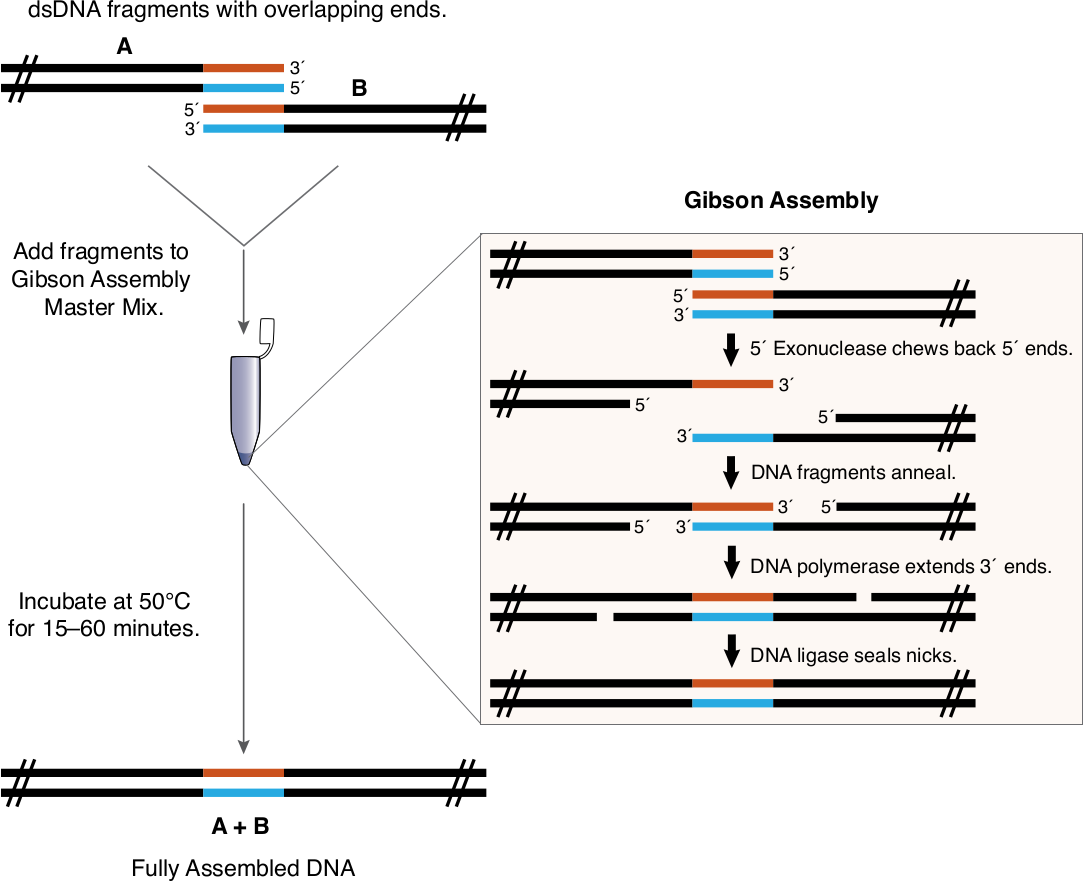
\includegraphics[width=0.8\textwidth, resolution=600, keepaspectratio=true]{graphics/gibson.png}}
			\caption[Overview of the Gibson assembly method]{Overview of the Gibson assembly method. Picture reproduced from the NEB Gibsson assembly master mix instruction manual NEB \#E2611S/L}
			\label{fig:gibson}
			\end{figure}				
		
		Once fragments of the desired size were obtained, the three PCR products were purified using the GE Healthcare Life Sciences Illustra-GRX PCR DNA and gel band purification kit and the concentration of DNA in the solution was estimated using the Nanodrop instrument. Simultaneously suicide plasmid vector pKAE604 was digested using Hind III and Sal I restriction enzymes. The digested product was purified and the concentration of the plasmid DNA was measured. For Gibson assembly NEB recommends a total DNA concentration of 0.2 to 1.0 pM when 4 to 6 DNA fragments are to be assembled. Therefore, for 4 fragments 0.25 pM is required and the weight in ng for each of the four fragments can be calculated with equation \ref{eq:gibson}. This allowed the volume required in $ \mu $l of the extracted DNA solutions to be determined. NEB recommends incubation of the Gibson Assembly master mix for an hour at 50\textcelsius.
		
		\begin{equation}
		\label{eq:gibson}
			weight \ in \ ng = \frac{pmols \times base \ pairs \times 650 \ daltons}{1000}
		\end{equation}
		
		\subsection{Transformation and validation}
		\label{sec:transformation}
		Following the Gibson assembly the ligated product was transformed into freshly prepared \textit{E. coli} DH5$ \alpha $ competent cells. As recommended by the NEB Gibson assembly protocol, the ligated product was diluted 4 fold (5 $ \mu $l of ligation in 15 $ \mu $l of deionised distilled water) prior to transformation. For transformation 2  $ \mu $l of the diluted product was added to 100  $ \mu $l of the competent cells and was held on ice for an hour. After an hour the cells were heat shocked for 90 sec at 42\textcelsius \ and then briefly returned to ice. The culture held on ice was mixed with 500  $ \mu $l of L-broth and was incubated at 37\textcelsius \ for an hour. Finally 200  $ \mu $l and 400  $ \mu $l of the culture was plated on to L-agar plates with kanamycin and grown at 37\textcelsius \ overnight.
		
		PCR was performed on the colonies picked from the transformation plates, using the left arm forward primer and the right arm reverse primer. The method for PCR was same as mentioned in the section \ref{sec:pcr} using the Taq polymerase enzyme. Table \ref{tab:validategibson} shows the PCR programme used for validating the ligation of the four fragments using Gibson assembly. The PCR product were analysed by 1 \% agarose gel electrophoresis. 

		\begin{table}[htbp]
		\caption{The PCR programme used for validating the product of Gibson assembly with the Taq DNA polymerase kit.}
		\label{tab:validategibson}
		\begin{center}
		\begin{tabular}{lrrr}
			\toprule[2pt]
			\textbf{Steps}          & \multicolumn{1}{l}{\textbf{Temperature (\textcelsius)}} & \multicolumn{1}{l}{\textbf{Time (sec)}} & \multicolumn{1}{l}{\textbf{Cycle}} \\ \midrule[1pt]
			Initial denaturation    &                                                      94 &                                      180 &                                  1 \\
			Denaturation            &                                                      94 &                                      30 &                                 30 \\
			Annealing and extension &                                                      72 &                                      90 &                                 30 \\
			Long extension          &                                                      72 &                                     600 &                                  1 \\ \bottomrule[2pt]
		\end{tabular}
		\end{center}
		\end{table}
		
		Successful PCR products were purified and sequenced using primers designed previously by Dr. Joanne Hothersall. Those primers bind on the region outside the multiple cloning site in the pAKE604 plasmid. The validated sample(s) was used to transform freshly prepared \textit{E. coli} S17-1 competent cells and were grown on L-agar plates with kanamycin selection and a sample of the successful transformant was stored in the -80\textcelsius \ freezer. 
		
		\subsection{Conjugal transfer of the suicide vector into \textit{P. fluorescens}}
		\label{sec:mating}
		For mating, overnight cultures were prepared for the transformed \textit{E. coli} S17-1 and the two \textit{P. fluorescens} host strains. 1 ml of each of the two \textit{P. fluorescens} host strains was mixed separately with 1 ml of the transformed \textit{E. coli} S17-1 strain. 1 ml of the culture mixture was filtered through a millipore nylon filter using a syringe and the filters were placed face up on to an L-agar plate without any antibiotic and grown overnight at 30\textcelsius. The bacteria were washed off the filters with 1 ml of saline. 10$ ^{-5} $ fold serial dilutions were made using 100 $\mu$l of the cells washed in saline followed by plating 100 $\mu$l of each dilution onto minimal medium plates with kanamycin selection. The plates were grown at 30\textcelsius \ for three to four days till the colonies were visible and big enough to be picked easily.
		
		To detect the successful transfer of the plasmid into the \textit{P. fluorescens} $ \Delta $ACP4 and $ \Delta $MupH cells, colonies were subjected to PCR (as described in Table \ref{tab:validategibson}) with ACP-K24a specific primers using Taq DNA polymerase.  The PCR products were analysed using 1\% agarose gel.
			 
		\subsection{Sucrose selection and excisant validation}
		\label{sec:suc selection}
		After mating, the \textit{P. fluorescens} \textit{trans} conjugants were subject to sucrose selection. For the \textit{P. fluorescens} $ \Delta $ACP4 trans-conjugants, colonies were grown overnight in L-broth without any selection. For each of the overnight cultures, five serial dilutions of 10$ ^{-1} $ were made for a final dilution of 10$ ^{-5}$  and 100 $\mu$l of culture from each of the five dilution tubes was plated on L-agar plates with sucrose selection. The cells were grown at 30\textcelsius \ for 24 hrs. To confirm that the plasmid had successfully excised out of the \textit{P. fluorescens} strains, colonies were patched onto two plates carrying ampicillin and kanamycin respectively. The colonies which grew on the ampicillin plates but not on the kanamycin plates were the ones which had successfully excised the plasmid. Successful excisions were subjected to PCR (as described in Table \ref{tab:validategibson}) with ACP-K24a specific primers using Taq DNA polymerase, in order to detect the integration of the ACP-K24a into \textit{P. fluorescens} $ \Delta $ACP4 chromosome.

		The previous steps validated the integration of the ACP-K24a into the \textit{P. fluorescens} $ \Delta $ACP4 chromosome but did not detect whether the integration had happened at the correct position in the \textit{mup} cluster. To validate that ACP-K24a had integrated at the correct position another PCR using Taq DNA polymerase was carried out. Primers designed previously by Dr. Anthony Haines, which bind to the positions outside the left and right arms were used with the annealing temperature of 53\textcelsius \ (as described in Table \ref{tab:validategibson}, with separate annealing and extension steps). \textit{P. fluorescens} NCIMB 10586 and \textit{P. fluorescens} $ \Delta $ACP4 were used as the controls. The PCR products were further subjected to restriction digests using enzymes Blp I and Stu I. Blp I cuts in the middle of the ACP-K24a but not does not cut anywhere in ACP-mupA3a and Stu I cuts in the middle of the ACP-mupA3a as well as at the rear ends of the two arms. A 20$\mu$l restriction digestion reaction mixture consists of DNA (5$\mu$l), Buffer (2$\mu$l), BSA (1$\mu$l), enzyme (conc. 5 units/$\mu$l) and enough sterile distilled water to make the total volume of 20$\mu$l. The restriction digest fragments were analysed by electrophoresis on 1\% agarose gel, an uncut fragment was used as the control. 
		
		For \textit{P. fluorescens} $ \Delta $MupH trans-conjugants sucrose selection was performed following the same steps as that for the \textit{P. fluorescens} $ \Delta $ACP4 trans-conjugants. However, to validate the excisions and integrants, samples were subjected to PCR using the primers designed to bind to the region outside the two arms. The steps of PCR with ACP-K24a specific primers and subsequent restriction digestions were excluded, since running a PCR using only the outer primers and sequencing the PCR products gave the same result in fewer steps and less time as compared to the above mentioned steps. 

		\subsection{Overlay Bioassay for \textit{in trans} expression of MupH, BatC and BatC L218M mutant}
		\label{sec:bioassay}
	
		For the bioassay 20 ml measured L-agar plates were made. The \textit{P. fluorescens} $ \Delta $H-6d strain carrying one of MupH, BatC or Batc L218M \textit{in trans} and the $ \Delta $4-1a  strain carrying the BatC \textit{in trans} were grown overnight in 5 ml L-broth with ampicillin selection. \textit{P. fluorescens} NCIMB 10586, $\Delta $MupH,  $ \Delta $ACP4, $ \Delta $H-6d and $ \Delta $4-1a were also grown without any plasmids, as controls. 100 $\mu$l of the overnight cultures were diluted with 900 $\mu$l of L-broth. To keep the concentration of the cells the same in all the cultures, the optical density of the samples was measured at 600 nm. Using equation \ref{eq:ODbioassay}, further dilutions were made keeping the total volume of the sample as 1 ml. 
		
		\begin{equation}
		\label{eq:ODbioassay}
		volume \ of \ the \ sample \ to \ dilute = \frac{smallest \ OD_{600}}{individual \ sample  \ OD_{600}} \times 1000
		\end{equation} 
		
		10 $ \mu $l of the diluted samples were spotted onto the 20 ml L-agar plates and were grown for 24 hr on the bench at room temperature. Simultaneously an overnight culture of \textit{Bacillus subtilis} 1064 strain was grown at 37\textcelsius. To prepare the overlay medium 4 ml of \textit{Bacillus subtilis} culture were mixed in 100 ml of molten L-agar and 500 $ \mu $l of TTC (5\% w/v). 15 ml of the overlay medium were poured over the spots from the 24 hr grown \textit{P. fluorescens} strains and were allowed to settle till the agar solidified, followed by a 24 hr incubation at 30\textcelsius. The diameters of the clearance zones were measured in two different directions, subtracting the diameter of the central disk. 
		  
		\subsection{High performance liquid chromatography analysis}
		\label{sec:hplc}
		To order to detect the pseudomonic acids produced by the \textit{in trans} expression of \textit{mupH}, \textit{batC} and \textit{batC} L218M in the ACP-K24a mutant \textit{P. fluorescens} strains, high performance liquid chromatography (HPLC) \nomenclature{HPLC}{High performance liquid chromatography} was performed. \textit{P. fluorescens} NCIMB 10586 and \textit{P. fluorescens} $ \Delta $H-6d and $ \Delta $4-1a with an empty pJH10 plasmid were used as controls. The seed cultures were prepared by growing the strains for 16 hr in L-broth at 25\textcelsius, 200 rpm. From the seed cultures, 1.25 ml of each sample was inoculated into  25 ml of the secondary stage medium (SSM). The inoculated cultures were grown at 22\textcelsius, 200 rpm for 40 hr. The cultures were pelleted in Falcon tubes by centrifugation at 5000 X g, at 25\textcelsius \ for 40 min. The supernatant was separated and filtered using 0.2 $ \mu $m Acrodiscs Nylon filters (Pall-Gelman, labs) before injection into the HPLC machine.
		
		The HPLC machine (Gilson) was supplied with HPLC grade water (Fisher) and 100\% aceto nitrile (Fisher) as mobile phase. The two solvents were added with 0.01\% formic acid (v/v) for pH adjustment and were degassed using an aspirator to remove any dissolved air prior to injection into the machine. The machine was set at 0.002 AUFS  (absorbance units full scale) \nomenclature{AUFS}{Absorbance units full scale} sensitivity and the detection was carried out at the wavelength of 233 nm. A Supelco reverse phase C18 column (15cm X 4.6 mm, 5$ \mu $m), which had hydrophobic alkyl chains covalently attached to the silica beads, was used to bind the hydrophobic compounds. Elution was performed by using a 5-70\% acetonitrile-water gradient at 1ml/min flow rate for 1 hr. Unipoint software was used to run the programme and analyse the chromatograms. 
		
		
		
		
		
		
		
		
		
		
		
		
		
\chapter{ACP-HCS interaction in \bet-branching}
\label{cha:ACP-HCS}

\section{Introduction}
\label{sec:IntroACP-HCS}
Some type I Polyketide biosynthesis systems, for example producing mupirocin, thiomarinol, kalamanticin, or myxovericins, are found to incorporate a branch on the third (i.e. \bet) carbon in the growing polyketide chain, referred to as a \bet-branch. This \bet-branching mechanism is thought to be catalysed via an \textquotedblleft HMG-CoA synthase (HCS) cassette\textquotedblright, consisting of an HMG-CoA synthase homologue and further auxiliary enzymes. In the mupirocin system the HCS cassette is a set of 5 proteins of which MupH (the HMG-CoA synthase homologue) is the first enzyme to interact with an acyl carrier protein (ACP) from the MmpA subunit. This interaction between ACP and MupH initiates the \bet-branching reaction. 

At the start of the present work little was known about the HCS cassette structure and function or how it interacts with the proteins in PKS? It was not understood what allows MupH to recognize the ACPs with substrates for \bet-branching, as opposed to the several other ACPs involved in a typical PKS pathway where branching is not required. We also did not know whether HCS proteins have a subtype or if they always work as one set of only five proteins as found in the mupirocin cluster. However, a recent study of the myxovirescin system \parencite{Simunovic2006} shows two HCS clusters involved in \bet-branching at two position in the synthesis pathway. These two stages are catalysed by two non-complimentary pairs of HMG-CoA synthase homologue and ACP interactions, which suggests the possibility of HCS subtypes. In a study of the curacin system, it was found that the HCS proteins can also work in conjunction with a halogenase. This halogenase activity adds a halogen (chlorine in case of curacin) on the $4^{th}$ ($ \gamma $-carbon) carbon of the growing polyketide chain \parencite{Busche2012}. 

A number of questions arise.
\begin{inparaenum}[\itshape 1\upshape)]
\item How different are the ACPs which interact with the HCS cassette from other ACPs found in the pathway? 
\item Is it possible to predict the molecular features responsible for the ACP-HCS recognition? 
\item And can these molecular features be exploited for the engineering of \bet-branching function in mupirocin biosynthesis pathway or other systems?
\end{inparaenum}
I have used computational methods to address these exciting questions. The work started using the preliminary data available from Prof. Christopher M. Thomas lab. 

In a sequence analysis carried out by Dr. Anthony Haines on the ACPs from various PKS systems, in \bet-branching ACPs a conserved tryptophan motif is found (Figure \ref{fig:WflagAlignment}) at the position 6 residues downstream of the catalytic serine. This position is not found to be conserved in the non-branching ACPs. It was also found that upon mutating this conserved tryptophan to leucine in the mupirocin system the production of pseudomonic acid A is significantly lowered. Thus, it was hypothesized that this conserved tryptophan could be the recognition motif. These preliminary observations lead Dr. Mathew Crump from the University of Bristol to solve the solution structure of the ACP di-domain from module 6 of the MmpA subunit in the mupirocin biosynthesis pathway. This NMR structure (PDB ID 2L22) has been used in the present work to carry out the predictions on the ACP-HCS interaction mechanism.

	\subsection{HMG-CoA synthase cassette}
	\label{sec:HMG-Coasynthase}
	The HCS cassette in the mupirocin biosynthesis pathway, is a set of 5 proteins consisting of an ACP (mACPc), a 3-hydroxy-3-methylglutaryl-CoA (HMG-CoA) synthase homologue (MupH), a decarboxylase (MupG) and two proteins (MupJ, MupK) from the crotonase superfamily. MupH homologues, our focus here \parencite{Wu2007}, are found in various polyketide biosynthesis pathways and are thought to be involved in \bet-branching mechanisms along with the other enzymes in the HCS cassette. It is hypothesized that acyl carrier proteins from the ACP di-domain (ACP-mupA3a and ACP-mupA3b), in the MmpA subunit of the mupirocin biosynthesis pathway, make the first point of contact with the MupH, initiating the \bet-branching reaction. This interaction between the ACPs and MupH is thought to be governed by a set of specificity determinants in the interacting residue pairs, which allows the ACPs involved in the \bet-branching systems to recognise and interact with the proteins in the HCS cassette. To understand better what governs the interaction between the ACPs and MupH, a structural model of the ACP-mupH complex determined either through experimental or computational methods could help to design mutagenesis experiments. The solution structure for the ACP-mupA3ab di-domain has been recently resolved (PDB ID 2L22), however there is no structure available for MupH. To predict a reliable structure of MupH and to understand its structural properties it was necessary to first understand the structural properties and the reaction mechanism catalysed by its homologue HMG-CoA synthase.

		\subsubsection{HMG-CoA synthase reaction mechanism}
		\label{sec:HCSreact}
		HMG-CoA synthases (EC 2.3.3.10) are 42 KDa proteins found in a wide range of organisms from bacteria to mammals and play a central role in fatty acid, polyketide, and isoprenoid biosynthesis. The enzyme belongs to the thiolase superfamily and can be broadly classified into the bacterial isoforms, the eukaryotic cytosolic isoforms and the mammalian specific mitochondrial isoform \parencite{Shafqat2010}.
	
		HMG-CoA synthase catalyses a three step reaction that involves a conserved Cys-His-Glu catalytic triad and an acyl-enzyme intermediate. As in \textit{Enterococcus faecalis} HMG-CoA synthase (PDB Id 1X9E) the first step is a \textbf{deacetylation} of the substrate Ac-CoA, H233 is thought to act as a catalytic base or H-bond donor for the nucleophilic C111, which attacks the carbonyl carbon of Ac-CoA , thereby transferring the acetyl group to the Cys-S atom and releasing the reduced CoASH (Figure  \ref{fig:HMGCO-Areact}) \parencite{Steussy2005}.

		\setlength\fboxsep{5pt}
		\setlength\fboxrule{1.5pt}
		\begin{figure}[]
		\centering
		\fbox{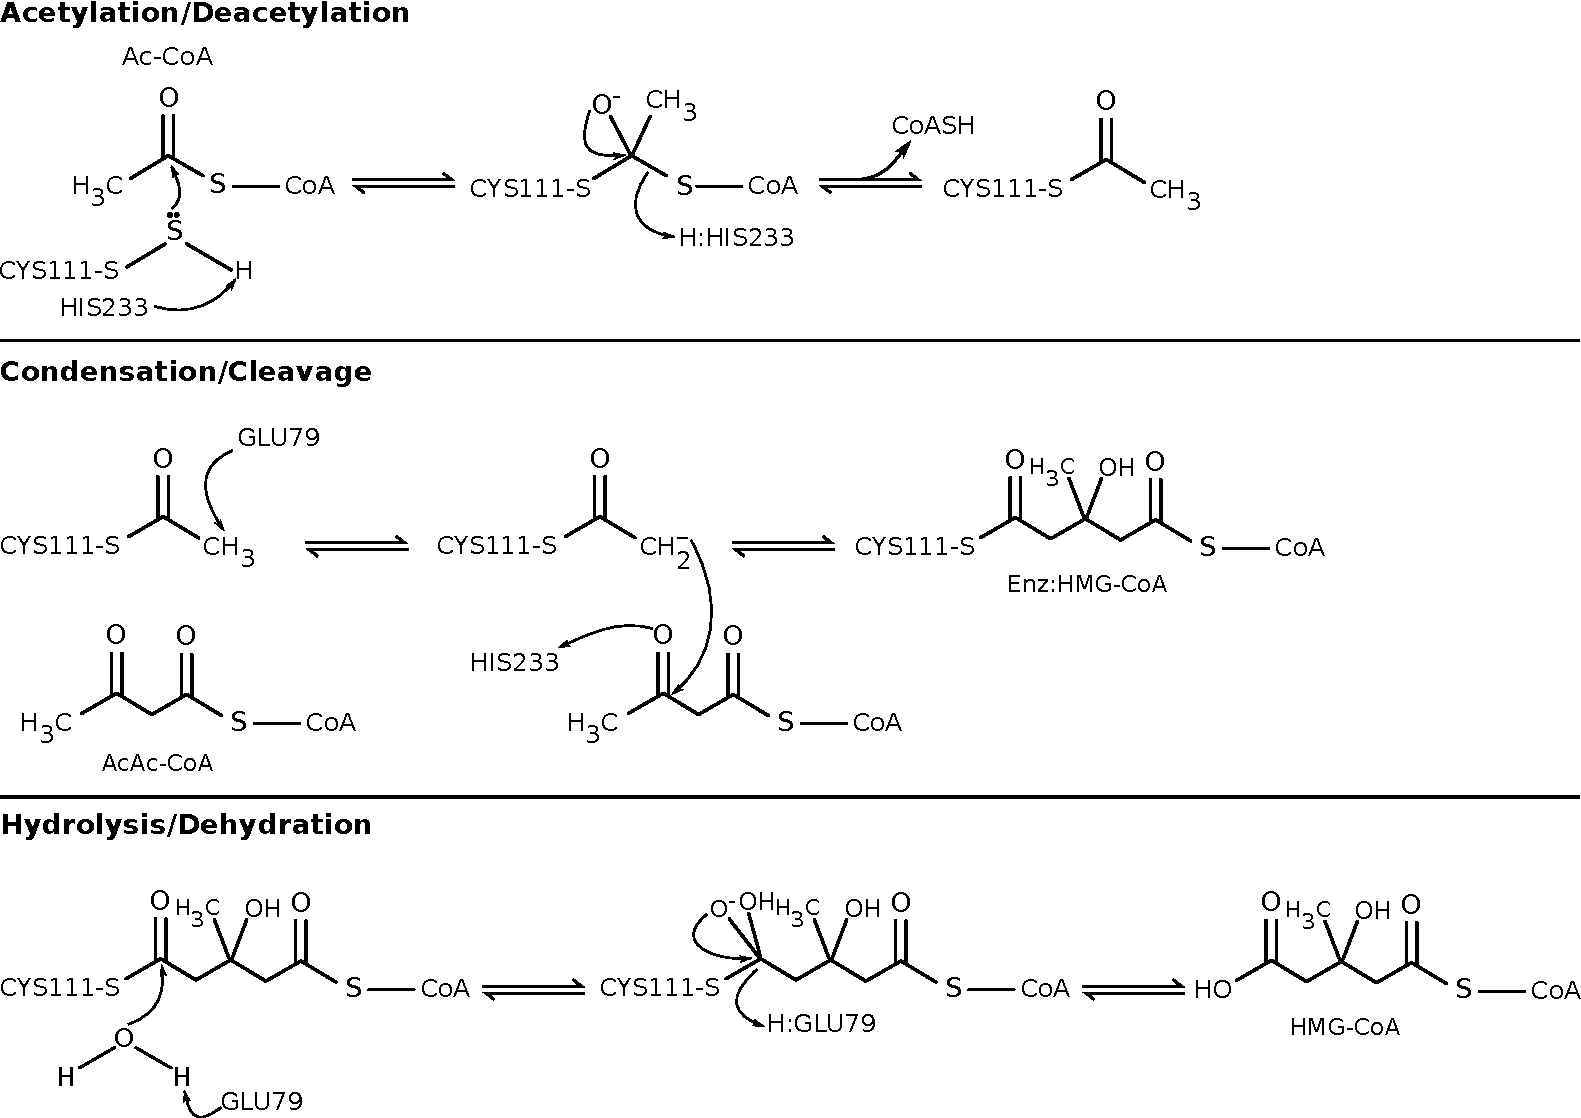
\includegraphics[width=0.9\textwidth, keepaspectratio=true]{graphics/hmgreact.pdf}}
		\caption[The reaction mechanism of HMG-CoA synthase.]{The reaction mechanism of HMG-CoA synthase. proposed in \parencite{Steussy2005}}.
		\label{fig:HMGCO-Areact}
		\end{figure}				
	
		In the second step, the methyl group of acetylated-Cys is deprotonated by the general base G79 to form a carbanion which attacks the distal (\bet) carbonyl of the incoming AcAC-CoA (second substrate), following the \textbf{condensation} of Ac-Co and AcAC-CoA forming an enzyme:HMG-CoA intermediate.
	
		In the final step the resultant enzyme:HMG-CoA intermediate is \textbf{hydrolyzed} to release the product HMG-CoA and regenerate the reduced Cysteine. G79 is shown to mediate the hydrolysis step. The similar reaction mechanism is also observed in \textit{Staphylococcus aureus, Brassica juncea} and Human HMG-CoA synthases \parencite{Theisen2004, Shafqat2010}.
		
		It is assumed that the \bet-branching mechanism of MupH would be similar to that of HMG-CoA synthase and thus can be used to guide the modelling.

\section{Results}

	\subsection{ACP sequence analysis}
	\label{sec: ACPSequenceAnalysis}
	The initial sequence analysis carried out by Dr. Anthony Haines on the seven well-characterized PKS clusters known to be involved in \bet-branching (Figure \ref{fig:WflagAlignment}) revealed the presence of a conserved tryptophan 6 residues downstream of the catalytic serine. A W was not seen at this position in the non-branching ACPs. Dr. Haines further used the sequence motif (DSXXXXXW) as a search pattern for PHI-BLAST and found further ACPs that he confirmed from the literature were associated with \bet-branching \parencite{Haines2013}. This sequence motif predicted ACPs from all the known systems involved in \bet-branching with the exception of two ACPs from virginiamycin and leinamycin clusters each. Which suggests that although this sequence motif is a strong predictor of \bet-branching associated ACPs it might not be enough to predict all of them. Therefore in the present study a stronger predictor, based on the statistical method of Hidden Markov models (HMM), was developed to classify ACPs into \bet-branching and non-\bet-branching types.
	
	\setlength\fboxsep{5pt}
	\setlength\fboxrule{1.5pt}
	\begin{figure}[]
	\centering
	\fbox{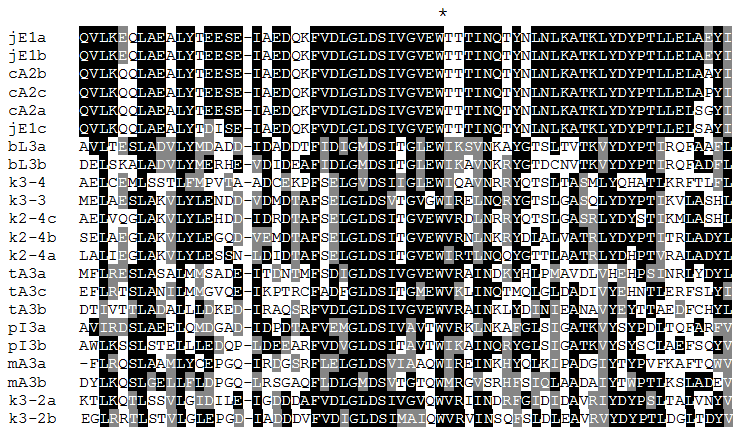
\includegraphics[width=0.9\textwidth, resolution=600, keepaspectratio=true]{graphics/wflagalignment.png}}
	\caption[Alignment of the ACP sequences from HCS cassette containing systems.]{Alignment of the ACP sequences from HCS cassette containing systems provided by Dr. Anthony Haines. The conserved W is indicated by a *.}
	\label{fig:WflagAlignment}
	\end{figure}
		
	 The sequences provided by Dr. Anthony Haines were used to build HMMs using 38 and 178 sequences from 15 well characterised pathways for the \bet-branching and non-\bet-branching ACPs respectively. These models were tested using a test set of ACPs (provided by Dr. Anthony Haines) from other clusters which were not part of the training set. These results were plotted on a graph of non-\bet-branching HMM score against \bet-branching HMM score (Figure \ref{fig:hmmplot}). The graph was divided by the $y=x$ line where the models predict an ACP as having the same likelihood of being a \bet-branching ACP or standard ACP. The majority of ACPs from the remaining clusters with at least one identified \bet-branch-associated ACP locate to one or other of these clusters (Figure \ref{fig:hmmplot}). 
	 
	 \bet-branching ACPs from the virginiamycin cluster were identified as the outliers which are just above the $ y=x $ line and adjacent to the \textquoteleft branching\textquoteright{ } cluster. Other outliers were the two \bet-branching ACPs from the leinamycin cluster one of which was just below the line and the other actually fallen within the non-branching cluster. Except for leinamycin, classifying ACPs using HMMs agrees with the available information about their likely presence in the \bet-branching or non-\bet-branching modules. The model for non-\bet-branching ACPs (standard) was used to fetch the ACP sequences from the UniProtKB/TrEMBL (20127441 seq) and Refseq microbial (6408654 seq) databases, database version on 9th March, 2012. I developed a couple of Perl scripts (see Appendix I) to remove all the sequences which were shorter than 60 aa or duplicates or sequences without the phosphopantethinylated serine which resulted in a set of 16,490 unique sequences. To ensure that these sequences cover the full length of the model, they were extended by 7 residues on both the ends. The extended sequences were scored using both the HMM models and a scatter diagram was plotted (Figure 3. Scatter diagrams showing the separation of ACPs into two clusters by their fit to the \bet-branch-associated \textquoteleft branching\textquoteright{ } ACP HMM and the non-branching \textquoteleft standard\textquoteright{ } ACP HMM. (b)). In Figure  \ref{fig:hmmplot} the scatter plots shows the separation of ACPs into two clusters by their fit to the \bet-branch-associated \textquoteleft branching\textquoteright{ } ACP HMM and the non-branching \textquoteleft standard\textquoteright{ } ACP HMM. These scatter plots were rendered by Dr. Anthony Haines using the data provided by the HMM analysis carried out by Rohit Farmer (this graph is also presented in \parencite{Haines2013}). 

	\setlength\fboxsep{5pt}
	\setlength\fboxrule{1.5pt}
	\begin{figure}[]
	\centering
	\fbox{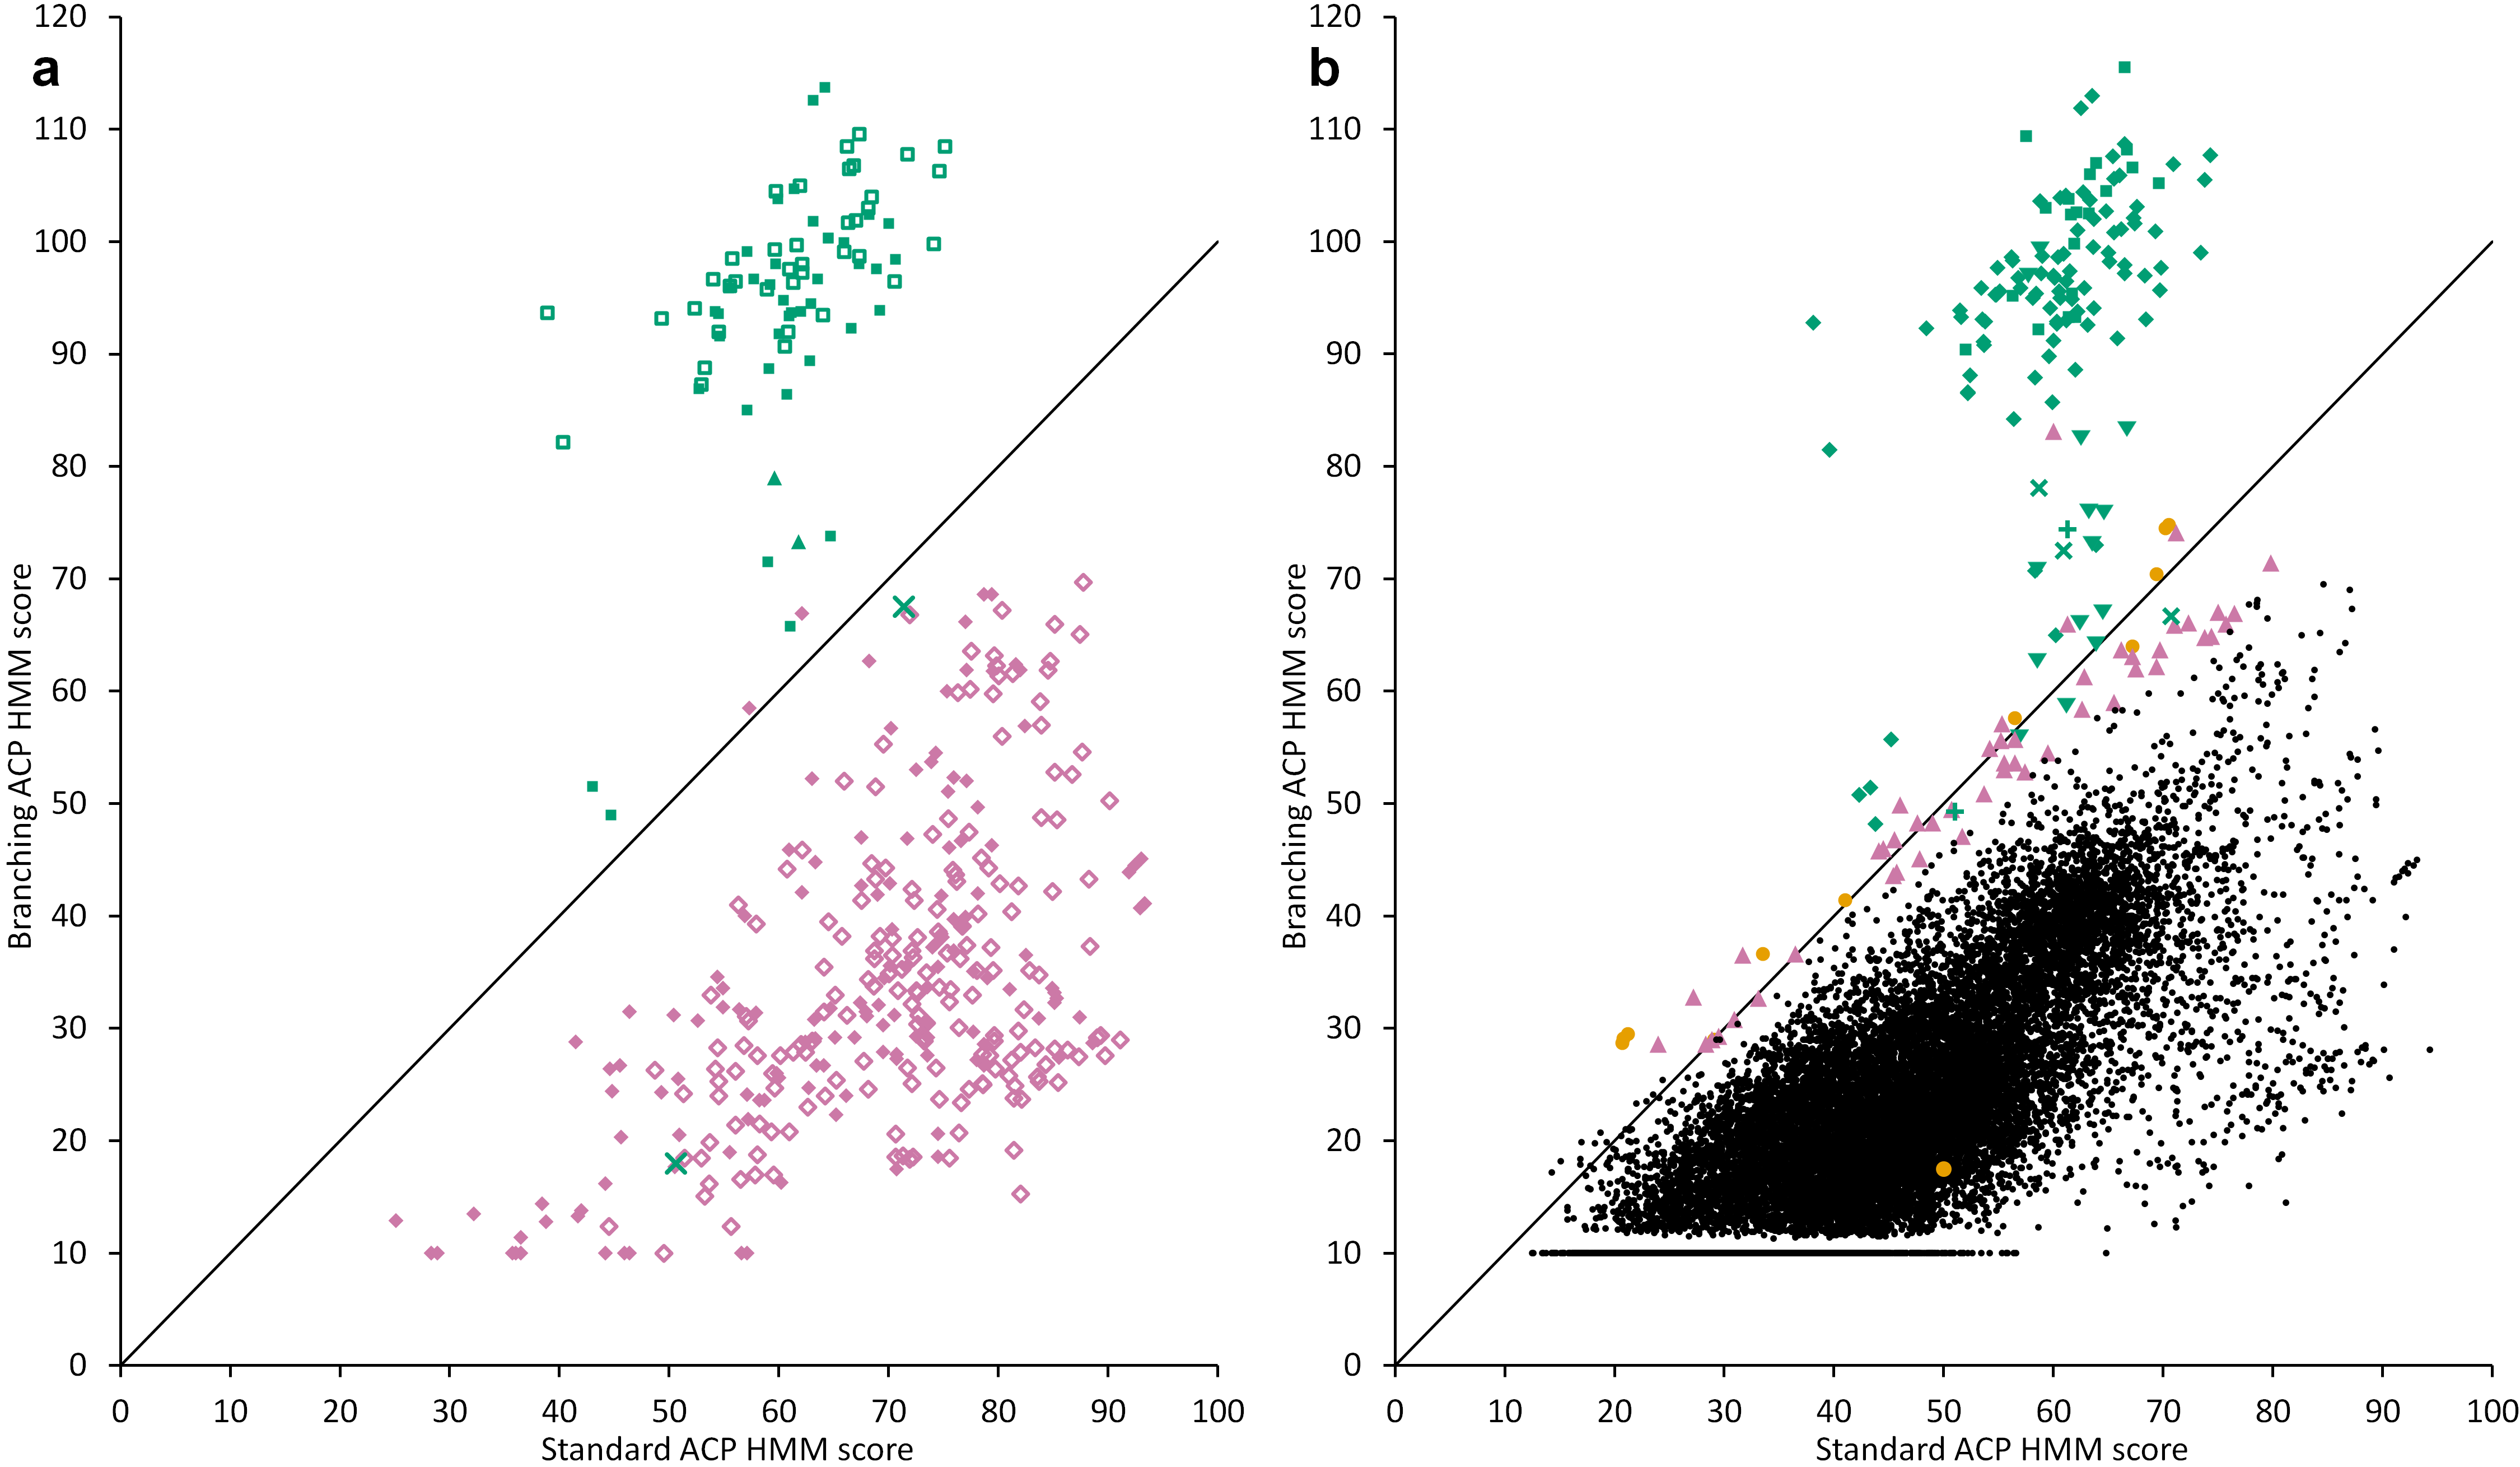
\includegraphics[width=0.9\textwidth, resolution=600, keepaspectratio=true]{graphics/hmmplot.png}}
	\caption[Scatter diagrams showing the separation of ACPs into two clusters by their fit to the \bet-branch-associated ‘branching’ ACP HMM and the non-branching ‘standard’ ACP HMM.]{Scatter diagrams showing the separation of ACPs into two clusters by their fit to the \bet-branch-associated ‘branching’ ACP HMM and the non-branching ‘standard’ ACP HMM. (A) ACPs from 26 pks clusters with at least one known or predicted branching ACP. (\textcolor{PineGreen}{$ \square $}) Training set for HMM using known branching ACPs. (\textcolor{PineGreen}{$ \blacksquare $}) predicted branching except (\textcolor{PineGreen}{$ \blacktriangle $}) virginiamycin cluster branching ACPs and (\textcolor{PineGreen}{$ \times $}) leinamycin cluster \bet-branch-associated module ACPs (\textcolor{Thistle}{$\lozenge$}) Training set for HMM using non-branching ACPs (\textcolor{Thistle}{$ \blacklozenge $}) predicted non-branching ACPs. (B) 16,490 ACP-like sequences identified by screening the TrEMBL and RefSeq protein databases using the standard ACP HMM. Sequences which did not pass the branching HMM cut-off were conferred a score of 10 so they could be plotted. (\textcolor{PineGreen}{$ \blacklozenge $}) branching ACP. (\textcolor{PineGreen}{$ \blacksquare $}) unlisted variants in similar clusters (\textcolor{PineGreen}{$ \times $}) known branching, (\textcolor{PineGreen}{$ \blacktriangledown $}) predicted branching, identified in this screen (\textcolor{PineGreen}{$ + $}) ACPs which may add branches in a non-type I-pks pathway. (\textcolor{Dandelion}{\textbullet}) insufficient sequence context or conflicting information. (\textcolor{Thistle}{$ \blacktriangle $}) predicted non-branching ($ \cdotp $) not examined. Graph and parts of the figure legend copied from \textcite{Haines2013}.}
	\label{fig:hmmplot}
	\end{figure}
		
	The newly found ACPs in the screen could be classified as likely \bet-branching or non-branching. On the graph, close to the $ y=x $ line, an HMM score of above 45 represents the ambiguous regions where the branching state of an ACP cannot be predicted below 45 seems to be indicative of non branching. One ACP from the leinamycin cluster was found in this region, the other in the non-branching region. The two \bet-branching ACPs from the myxovirescin, cluster, which are associated with different MupH homologues, can be clearly identified. This suggests that the HMM model can be used to identify the ACPs associated with the \bet-branching but cannot be used to predict the ACP subtypes if they exist.
			
		\subsubsection{Minimum changes required to shift ACP-tmlD3a from non-\bet-branching to \bet-branching cluster.}
		\label{sec:MinumChanges}
		It was observed in the HMM analysis that the \bet-branching ACPs and the non-\bet-branching ACPs (standard) cluster in different zones, which raises a question as to the minimum changes necessary to shift an ACP from standard ACP cluster to \bet-branching ACP cluster, as scored by the HMM models? These mutations might allow us to make a non-branching ACP function like a \bet-branching ACP.
				
		To address this question I wrote a Perl script (Appendix I, Script \ref{sec:MinChangesScript}) to mutate each and every position in the sequence to the other 19 proteinogenic amino acids. A non branching ACP (ACP-tmlD3a) from the thiomarinol cluster was taken as the sequence of reference. ACP-tmlD3a was chosen because experiments from Prof. Thomas group showed no mupirocin production upon replacing ACP-mupA3a/b with ACP-tmlD3a/b. The script generated all possible substitutions at each of the 67 positions in the sequence, giving 19 X 67  = 1273 sequences.
	
		\setlength\fboxsep{5pt}
		\setlength\fboxrule{1.5pt}
		\begin{figure}[]
		\centering
		\fbox{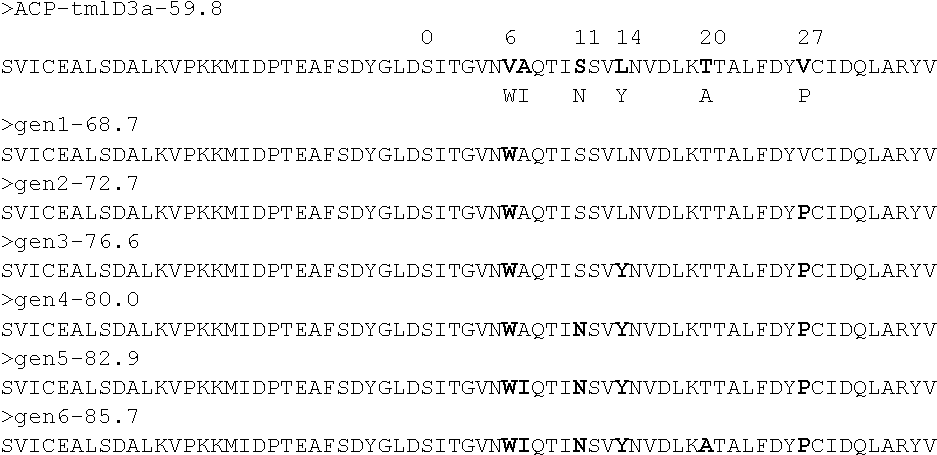
\includegraphics[width=0.9\textwidth, resolution=600, keepaspectratio=true]{graphics/minchanges.pdf}}
		\caption[The number of mutations required to reach the score of 82.2 or above when scored with \bet-branching HMM model.]{The ACP-tmlD3a sequence scored 59.8 against \bet-branching HMM model and would require 5 mutations at the positions 6, 7, 11, 14 , and 20 counting from the active site serine (0) to reach the score 82.9 and 6$^{th}$ mutation at position 27 to score 85.7. Figure  3 .9 shows the relative positions of the residues required to be mutated on the ACP-tmlD3a:MupH complex}
		\label{fig:minchanges}
		\end{figure}
					
		From the previous analysis it was observed that the \bet-branching ACP sequences typically score in the range of 82.2 to 109.6 using \bet-branching HMM model (wacp.hmm). This suggests that if any sequence scores 82.2 or above using \bet-branching HMM model, should fall under the \bet-branching cluster. Utilizing this observation the 1273 sequences were scored using \bet-branching model %(wacp.hmm), 
		thus generating a first generation of mutated sequences. The sequence with the highest score was selected for the next generation of mutations and the process was iterated till a score of 82.2 or above was reached. For ACP-tmlD3a it took 5 generations (iteration) to reach the score of 82.9 and 85.7 in 6 generations. 
				
		This experiment suggests that it would need to make a minimum of 6 mutations at the positions shown in Figure \ref{fig:minchanges} and listed in Table \ref{tab:MinimumACPChanges}, to shift the ACP-tmlD3a from the non-branching ACP cluster to the \bet-branching ACP cluster. Unsurprisingly, the highest scoring amino acid change in the first generation of mutated sequences was tryptophan (W). All the other mutations were observed downstream from the active site serine are mainly towards helix III (Figure \ref{fig:minchangestd3a}). The same method could be applied to the other ACPs as well however, the number of mutations (iterations) required may be different.
				
				
				\begin{table}[htbp]
				\begin{small}
				\caption{Muations required for ACP-tmlD3a sequence to score more highly with the HMM trained on branching ACPs than with the non-branching ACPs}
				\label{tab:MinimumACPChanges}
				\begin{center}
				\begin{tabular}{c c c}
					\toprule[2pt]
					 Mutation  & Branching ACP HMM & Standard ACP HMM \\ \midrule[1pt]
					ACP-tmlD3a & 59.8              & 79.4             \\
					   V36W    & 68.7              & 76.1             \\
					   V57P    & 72.7              & 79               \\
					   L44Y    & 76.6              & 79.3             \\
					   S41I    & 80                & 80.1             \\
					   A37I    & 82.9              & 80.1             \\
					   T50A    & 85.7              & 78.9             \\ \bottomrule[2pt]
				\end{tabular}
				\end{center}
				\end{small}
				\end{table}
	
			\setlength\fboxsep{5pt}
			\setlength\fboxrule{1.5pt}
			\begin{figure}[]
			\centering
			\fbox{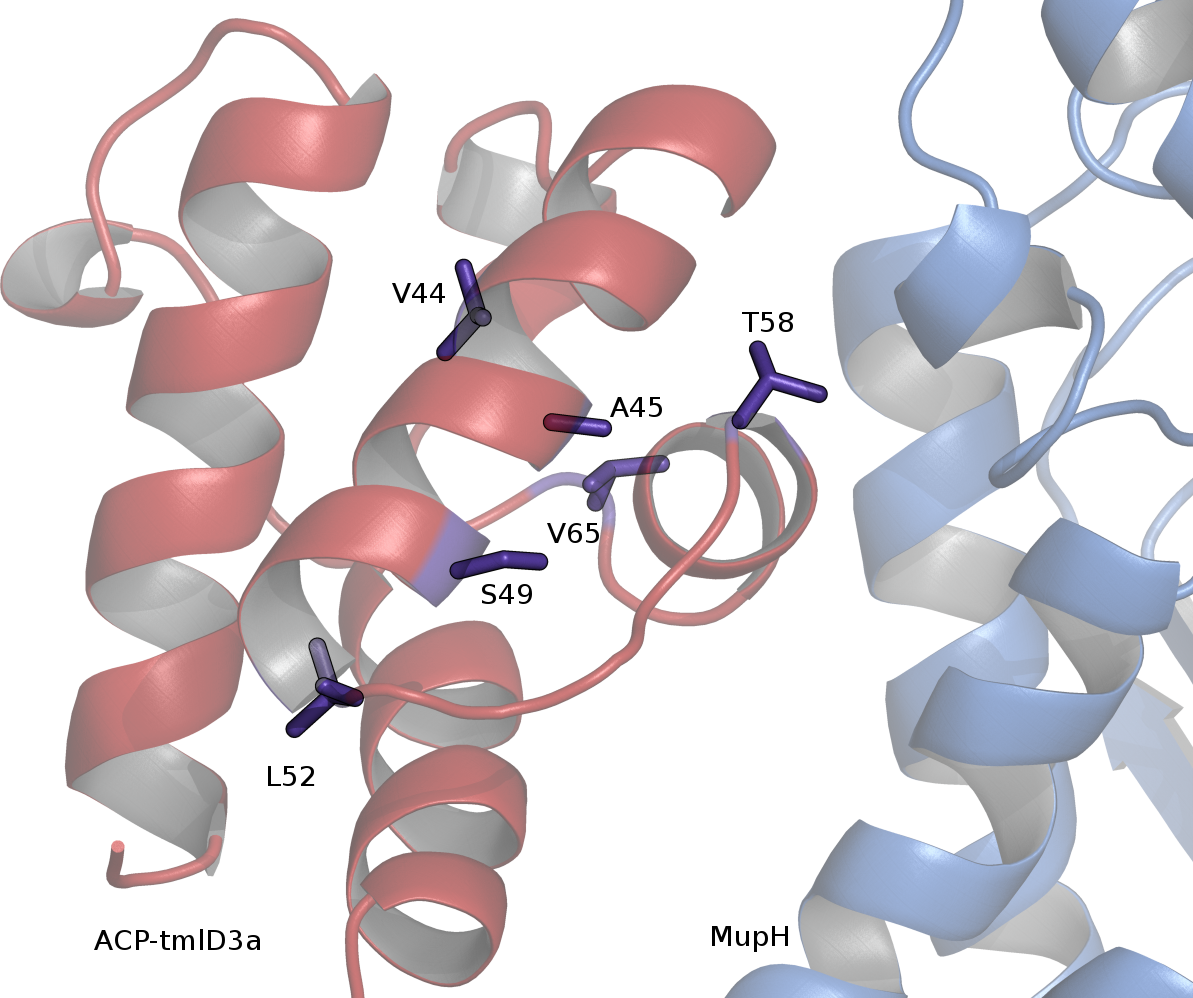
\includegraphics[width=0.7\textwidth, resolution=600, keepaspectratio=true]{graphics/minchangestd3a.png}}
			\caption[Mutations required reaching the score of 82.2 or above when scored with \bet-branching HMM model mapped on the structure.]{Mutations required reaching the score of 82.2 or above when scored with \bet-branching HMM model mapped on the structure. ACP-tmlD3a (red) in complex with MupH (Blue) superimposed on the mupA3a:MupH complex 1 from cluster 1. The residues displayed as sticks are the positions for the mutations V44W, V65P, L52Y, S49I, A45I and T58A that are needed for the ACP-tmlD3a sequence to score more highly in the HMM trained on \bet-branching ACPs than in the HMM trained on non-\bet-branching ACPs (see Table \ref{tab:MinimumACPChanges})}
			\label{fig:minchangestd3a}
			\end{figure}			
		
	\subsection{ACP structure analysis}
	\label{sec:ACPStructureAnalysis}
	%So it is clearly important for recognition, even though it was not intially clear how, the structure of the di-domain ACPs from the module 6 of the MmpA subunit in the mupirocin synthesis pathway was determined through NMR (PDB ID 2L22). 
	The NMR determined apo ACP-mupA3ab (PDB ID 2L22) structures consists of a typical four helical bundle. The NMR experiments showed that the conserved tryptophan identified in the sequence analysis lies buried in the ACPs core between helix I and helix II rather than forming an exposed patch. The burial of the tryptophan inside the ACP core raised the question of how this residue permits an interaction between the ACPs and the HMG-CoA synthase homologue. As mentioned earlier that on the basis of the W to L mutation experiments which showed a substantial decrease in the pseudomonic acid A production.
	
	The orientation of the tryptophan seen in ACP-mupA3a is almost perpendicular to  that in ACP-mupA3b, Figure \ref{fig:acp3and4} shows ACP-mupA3a and ACP-mupA3b superimposed on helix II, however, both the configurations are in trans Figure \ref{fig:acp3nmr} shows that the conformation of W is consistent with the ensemble for each ACP. Figure \ref{fig:2liunmr} shows the 20 NMR structures of an ACP homologue from the curacin system (PDB ID 2LIU). Figure \ref{fig:allacps} shows the structural comparison of the curacin ACPs (2LIU, 2LIW) with the mup ACPs. The tryptophan side chains can be seen to form a continuum rather than being biased towards a preferred orientation. Notably in all the above mentioned ACP structures the tryptophan side chain tends to orient similarly within a given NMR ensemble but is different between ensembles. However, the curacin ACP (2LIU and 2LIW) ensembles are more similar to each other than ACP-mupA3a and ACP-mupA3b to each other.  Table \ref{tab:RotamericValue} lists the rotameric values for the tryptophan side chain in the above mentioned four ACP structures. The tryptophan side chain atom numbering scheme is based on the Recommendations for the presentation of NMR structures of proteins and nucleic acids \parencite{Markley1998}. Another notable difference in the ACP-mupA3a/b structure is the position of the helix III (Figure \ref{fig:diffhelix3}).
	
	\begin{table}[htbp]
	\caption{Backbone dependent tryptophan side chain rotameric values}
	\begin{center}
	\begin{tabular}{p{1.5cm}p{1.5cm}p{1.5cm}p{1.5cm}p{1.5cm}p{1.5cm}}
	
		\toprule[2pt]
		ACPs & \multicolumn{1}{l}{Phi} & \multicolumn{1}{l}{Psi} & \multicolumn{1}{l}{Chi1} & \multicolumn{ 2}{c}{Chi2}   \\
	         & \multicolumn{1}{l}{\tiny(C$'_{i-1}$-N$_{i}$- C$^{\alpha}_{i}$-C$'_{i}$)} & \multicolumn{1}{l}{\tiny(N$_{i}$-C$^{\alpha}_{i}$-C$'_{i}$-N$_{i+1}$)} & \multicolumn{1}{l}{\tiny(N-C$^{\alpha}$-C$ ^{\beta} $-C$^{\gamma}$)} & \multicolumn{1}{l}{\tiny(C$^{\alpha}$-C$^{\beta}$-C$^{\gamma}$-C$^{\delta1}$)} & \multicolumn{1}{l}{\tiny(C$^{\alpha}$-C$^{\beta}$-C$^{\gamma}$-C$^{\delta2}$)} \\ \midrule[1pt]
	  mupA3a & -62   & -38.5 & -158.8 & 77.3 & -103.8  \\
	  mupA3b & -59.5 & -54.7 & -178.2 & 10.9 & -170.6  \\
	  2LIU   & -65.3 & -36.5 & -168.6 & 59.8 & -118.6  \\
	  2LIW   & -66.8 & -34   & -169.3 & 45.2 & -132.4  \\ \bottomrule[2pt]
	\end{tabular}
	\end{center}
	\label{tab:RotamericValue}
	\end{table}
			
	These measured rotamer values for the tryptophan side chain atoms were compared with the values given in the default set of the 2010 backbone-dependent rotamer library \parencite{Shapovalov2011} from Ronald Dunbrack's group. By looking into the Dunbrack’s rotamer library it was not obvious what causes the difference in the orientation of the tryptophan as the calculated values lie within the rotamer probability distribution. To supplement the observation the NMR structure of ACP-mupA3a/b had all side chains removed and the SCWRL4 software \parencite{Krivov2009}, which uses the Dunbrack rotamer library, was used to put the side chains back on the ACP backbone. SCWRL4 placed the side chains at similar positions to those of the original side chains in the NMR structure for both ACP-mupA3a/b, which suggests nothing unusual about the W residues.
	
			\setlength\fboxsep{5pt}
			\setlength\fboxrule{1.5pt}
			\begin{figure}[]
			\centering
			\fbox{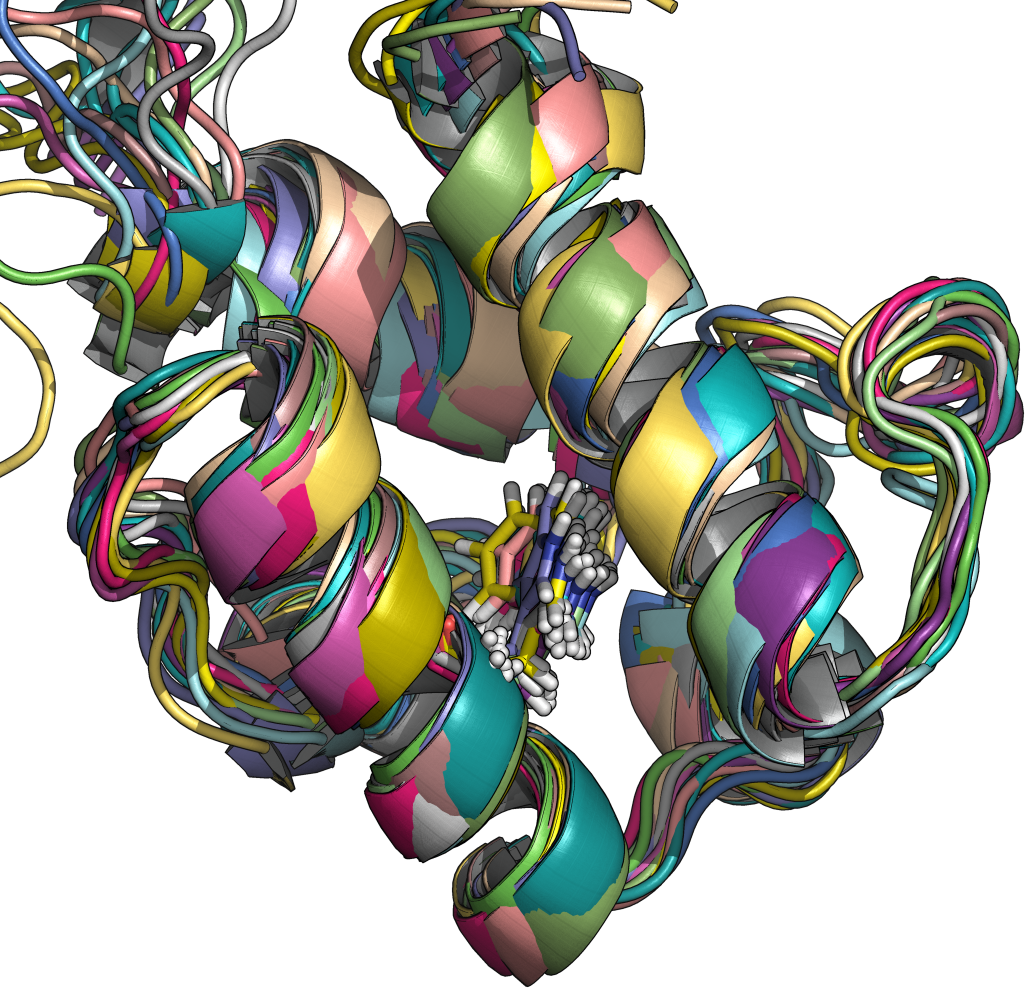
\includegraphics[width=0.6\textwidth, resolution=600, keepaspectratio=true]{graphics/acp3nmr.png}}
			\caption[The 20 ACP-mupA3a NMR models superimposed on each other. Tryptophan highlighted as sticks.]{The 20 ACP-mupA3a NMR models superimposed on each other. Tryptophan highlighted as sticks.}
			\label{fig:acp3nmr}
			\end{figure}			
	
			\setlength\fboxsep{5pt}
			\setlength\fboxrule{1.5pt}
			\begin{figure}[]
			\centering
			\fbox{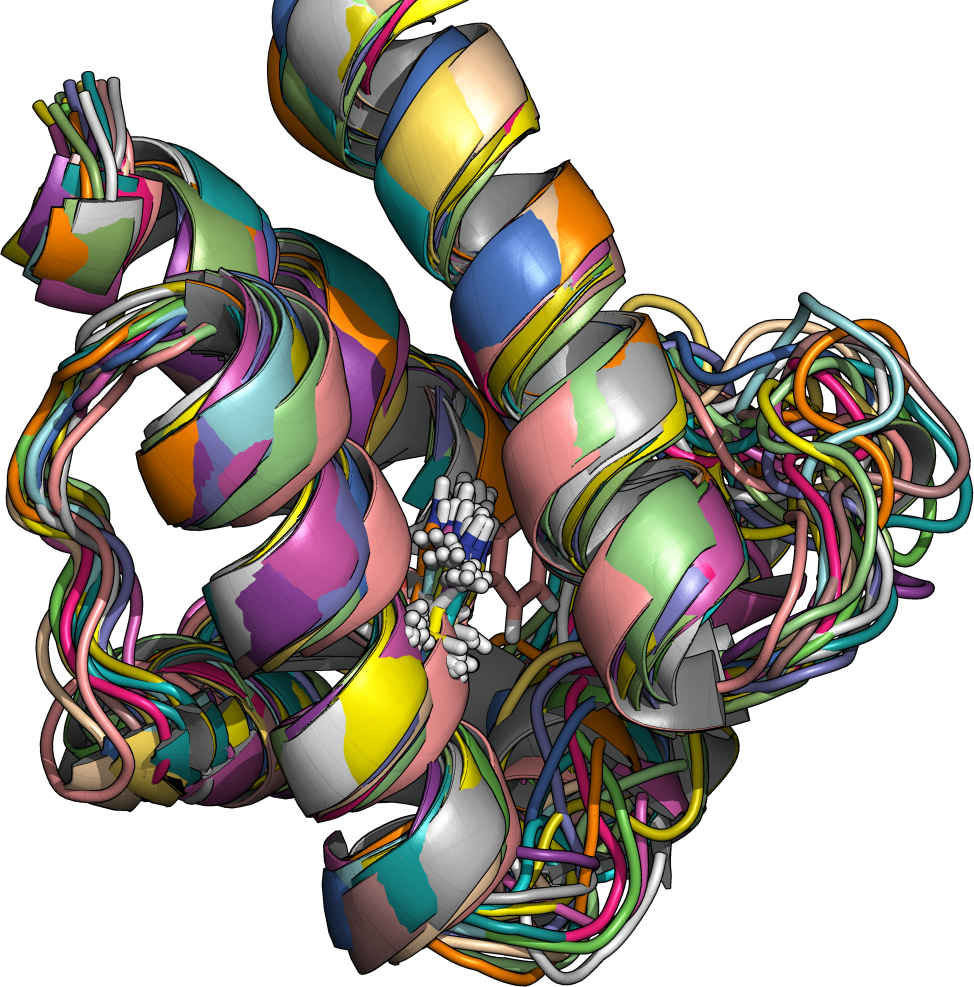
\includegraphics[width=0.6\textwidth, resolution=600, keepaspectratio=true]{graphics/acp4nmr.png}}
			\caption[The 20 ACP-mupA3b NMR models superimposed on each other. Tryptophan highlighted as sticks.]{The 20 ACP-mupA3b NMR models superimposed on each other. Tryptophan highlighted as sticks.}
			\label{fig:acp4nmr}
			\end{figure}					
	
			\setlength\fboxsep{5pt}
			\setlength\fboxrule{1.5pt}
			\begin{figure}[]
			\centering
			\fbox{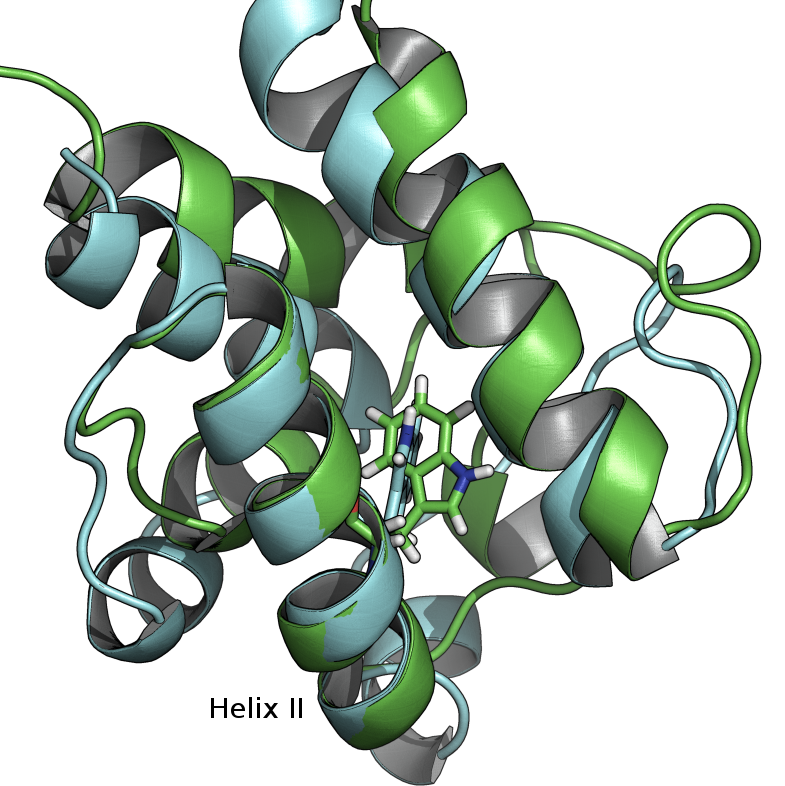
\includegraphics[width=0.6\textwidth, resolution=600, keepaspectratio=true]{graphics/acp3and4.png}}
			\caption[ACP-mupA3a (green) and ACP-mupA3b (cyan) superimposed on helix II. Tryptophan highlighted as sticks]{ACP-mupA3a (green) and ACP-mupA3b (cyan) superimposed on helix II. Tryptophan highlighted as sticks}
			\label{fig:acp3and4}
			\end{figure}							
			
			\setlength\fboxsep{5pt}
			\setlength\fboxrule{1.5pt}
			\begin{figure}[]
			\centering
			\fbox{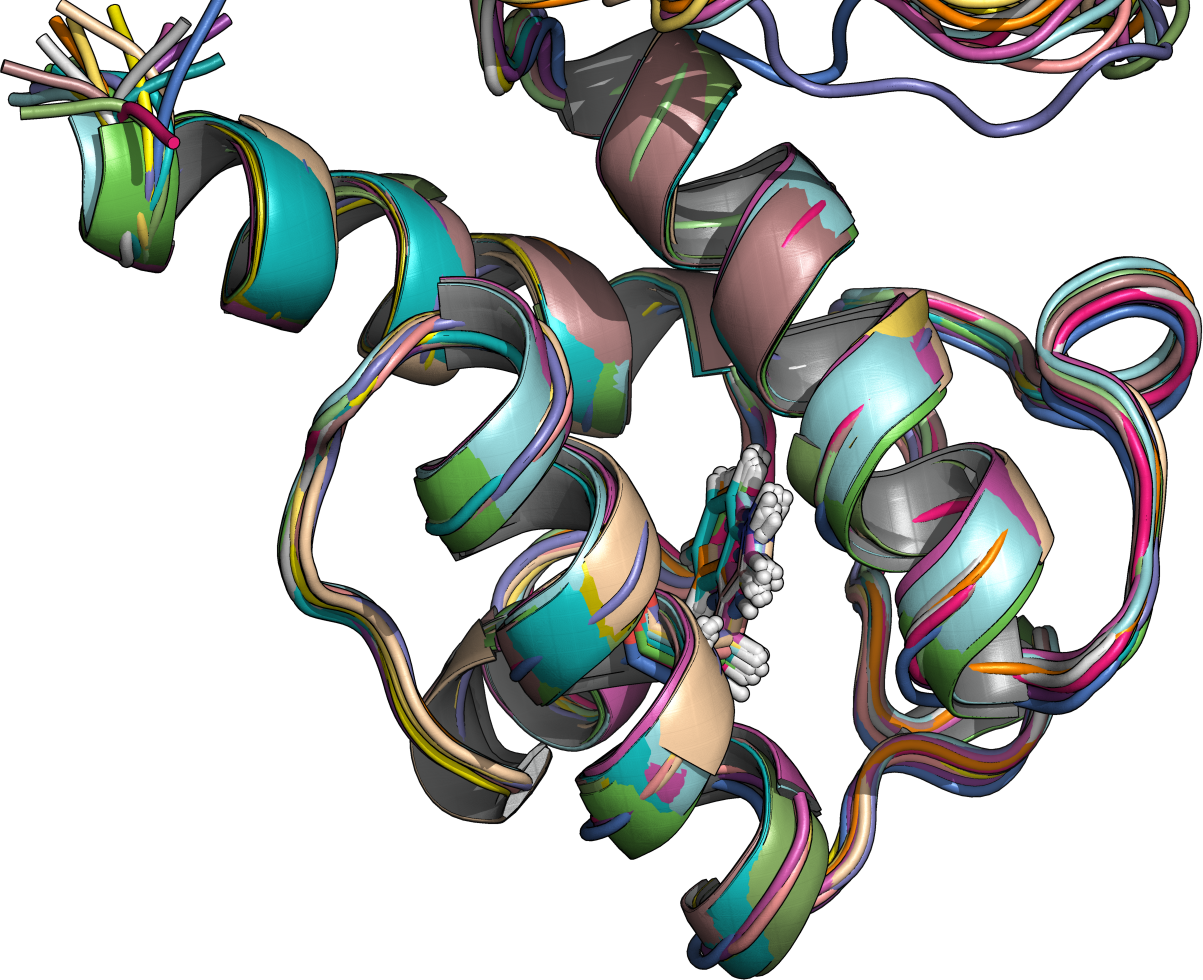
\includegraphics[width=0.6\textwidth, resolution=600, keepaspectratio=true]{graphics/2liunmr.png}}
			\caption[Curacin ACP responsible for halogenase activity via \bet-branching mechanism (PDB ID 2LIU), NMR models superimposed on each other. Tryptophan highlighted as sticks.]{Curacin ACP responsible for halogenase activity via \bet-branching mechanism (PDB ID 2LIU), NMR models superimposed on each other. Tryptophan highlighted as sticks.}
			\label{fig:2liunmr}
			\end{figure}
	
			\setlength\fboxsep{5pt}
			\setlength\fboxrule{1.5pt}
			\begin{figure}[]
			\centering
			\fbox{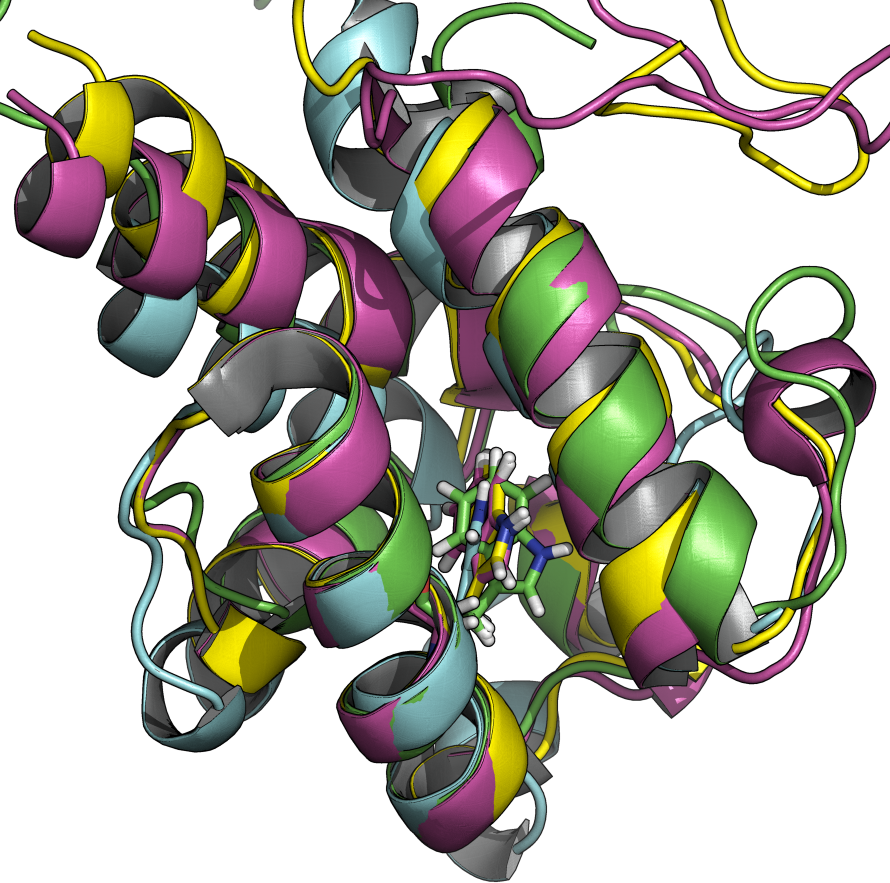
\includegraphics[width=0.6\textwidth, resolution=600, keepaspectratio=true]{graphics/allacps.png}}
			\caption[Superimposed representative structures of ACP-mupA3a (green), ACP-mupA3b (cyan), curacin ACPS 2LIU (magenta) and 2LIW (yellow).]{Superimposed representative structures of ACP-mupA3a (green), ACP-mupA3b (cyan), curacin ACPS 2LIU (magenta) and 2LIW (yellow). Tryptophan highlighted as sticks.}
			\label{fig:allacps}
			\end{figure}
	
			\setlength\fboxsep{5pt}
			\setlength\fboxrule{1.5pt}
			\begin{figure}[]
			\centering
			\fbox{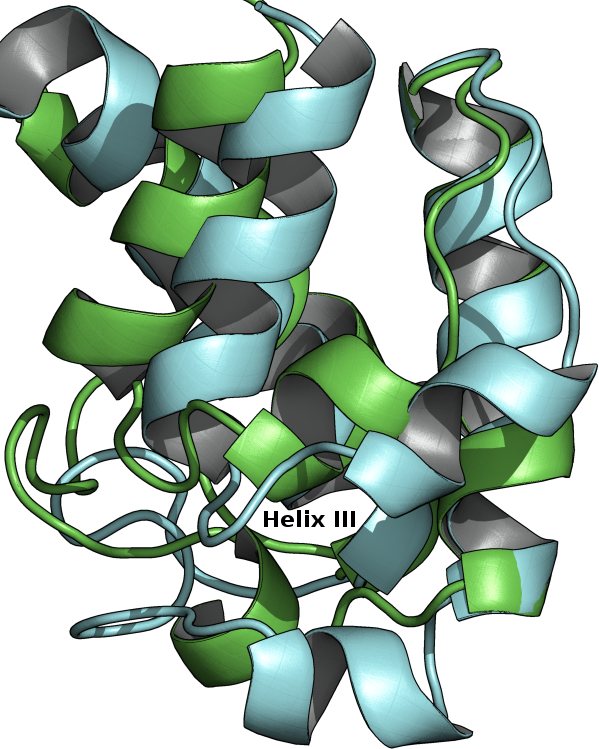
\includegraphics[width=0.4\textwidth, resolution=600, keepaspectratio=true]{graphics/diffhelix3.png}}
			\caption[Superimposed ACP-mupA3a (green) and ACP-mupA3b (cyan) highlighting the difference in helix III position.]{Superimposed ACP-mupA3a (green) and ACP-mupA3b (cyan) highlighting the difference in helix III position.}
			\label{fig:diffhelix3}
			\end{figure}
		
		\subsubsection{Affect of W to L mutation on ACP molecular dynamics}
		\label{sec:WtoLMD}
		To investigate the possible effect of the W to L mutation on the structural dynamics of ACP-mupA3a, molecular dynamics simulations of the wild type and mutant ACP in water were carried out (see methods section \ref{sec:WtoL_MD}) . Figure \ref{fig:MDacp} shows the averaged root mean square fluctuation (RMSF) of 20 simulations for wild and mutant type each. The RMSF values suggest significantly greater motion in the mutant than in the wild type, with the largest effects being around helix III and in the loop between helix I and helix II.
				
			\setlength\fboxsep{5pt}
			\setlength\fboxrule{1.5pt}
			\begin{figure}[]
			\centering
			\fbox{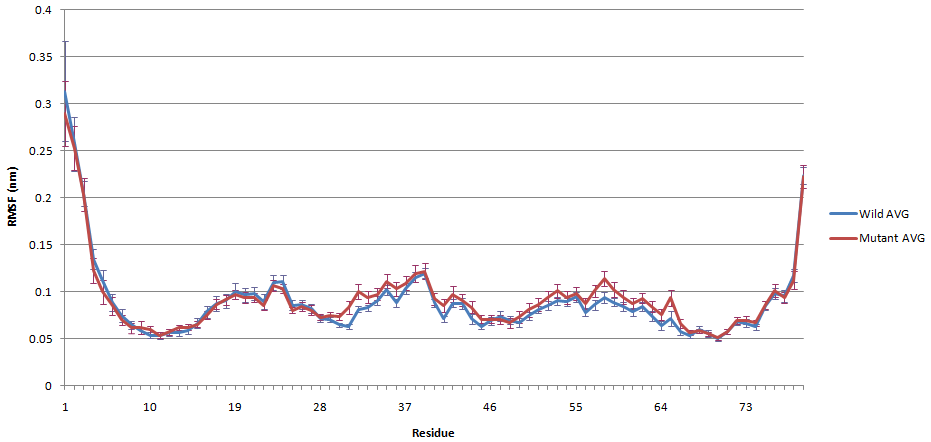
\includegraphics[width=0.9\textwidth, keepaspectratio=true]{graphics/MDacp.png}}
			\caption[Graph of the average over 20 simulations of the root mean squared fluctuation (RMSF) of the backbone calculated for each simulation of the wild type (blue) and W44L mutant (red) of ACP-mupA3a.]{Graph of the average over 20 simulations of the root mean squared fluctuation (RMSF) of the backbone calculated for each simulation of the wild type (blue) and W44L mutant (red) of ACP-mupA3a. The error bars represent the least significant difference at the 95\% confidence level; i.e. where the error bars of the two lines do not overlap they are signifcant in a t-test with 95\% confidence. Residues 29-35 (central part of the loop between helix I and helix II), 41, 44 (in helix II), 57-59 (N-ter of helix III), and 64 (C-ter of helix 3) show significantly greater motion in the mutant than in the wild type, with the largest effects being around helix III and in the loop between helix I and helix II. Graph reproduced from \textcite{Haines2013}.}
			\label{fig:MDacp}
			\end{figure}			

	\subsection{MupH structure prediction}
	\label{sec:MupHstructure}
	As the MupH structure was not available in the PDB database, homology modelling was used to predict its three dimensional structure. A structural homologue from \textit{Staphylococcus auereus} (PDB ID 1X9E) was used as the template for the protein structure prediction as well as for the docking of the mupirocin intermediate in the predicted structure (details in section \ref{sec:HomologyModellingMupH}). The predicted structures were verified for their stereochemical qualities and energy minimized to stabilise the docked ligand inside the active site (Figure \ref{fig:MupH}). To verify the correct orientation of the ligand inside the MupH active site the residues within 5 \AA{} of the docked ligand (Figure \ref{fig:5around}) were compared with conserved and functionally important residues in the MupH homologue structures (Figure \ref{fig:1XPKvsMupH} ).
	
			\setlength\fboxsep{5pt}
			\setlength\fboxrule{1.5pt}
			\begin{figure}[]
			\centering
			\fbox{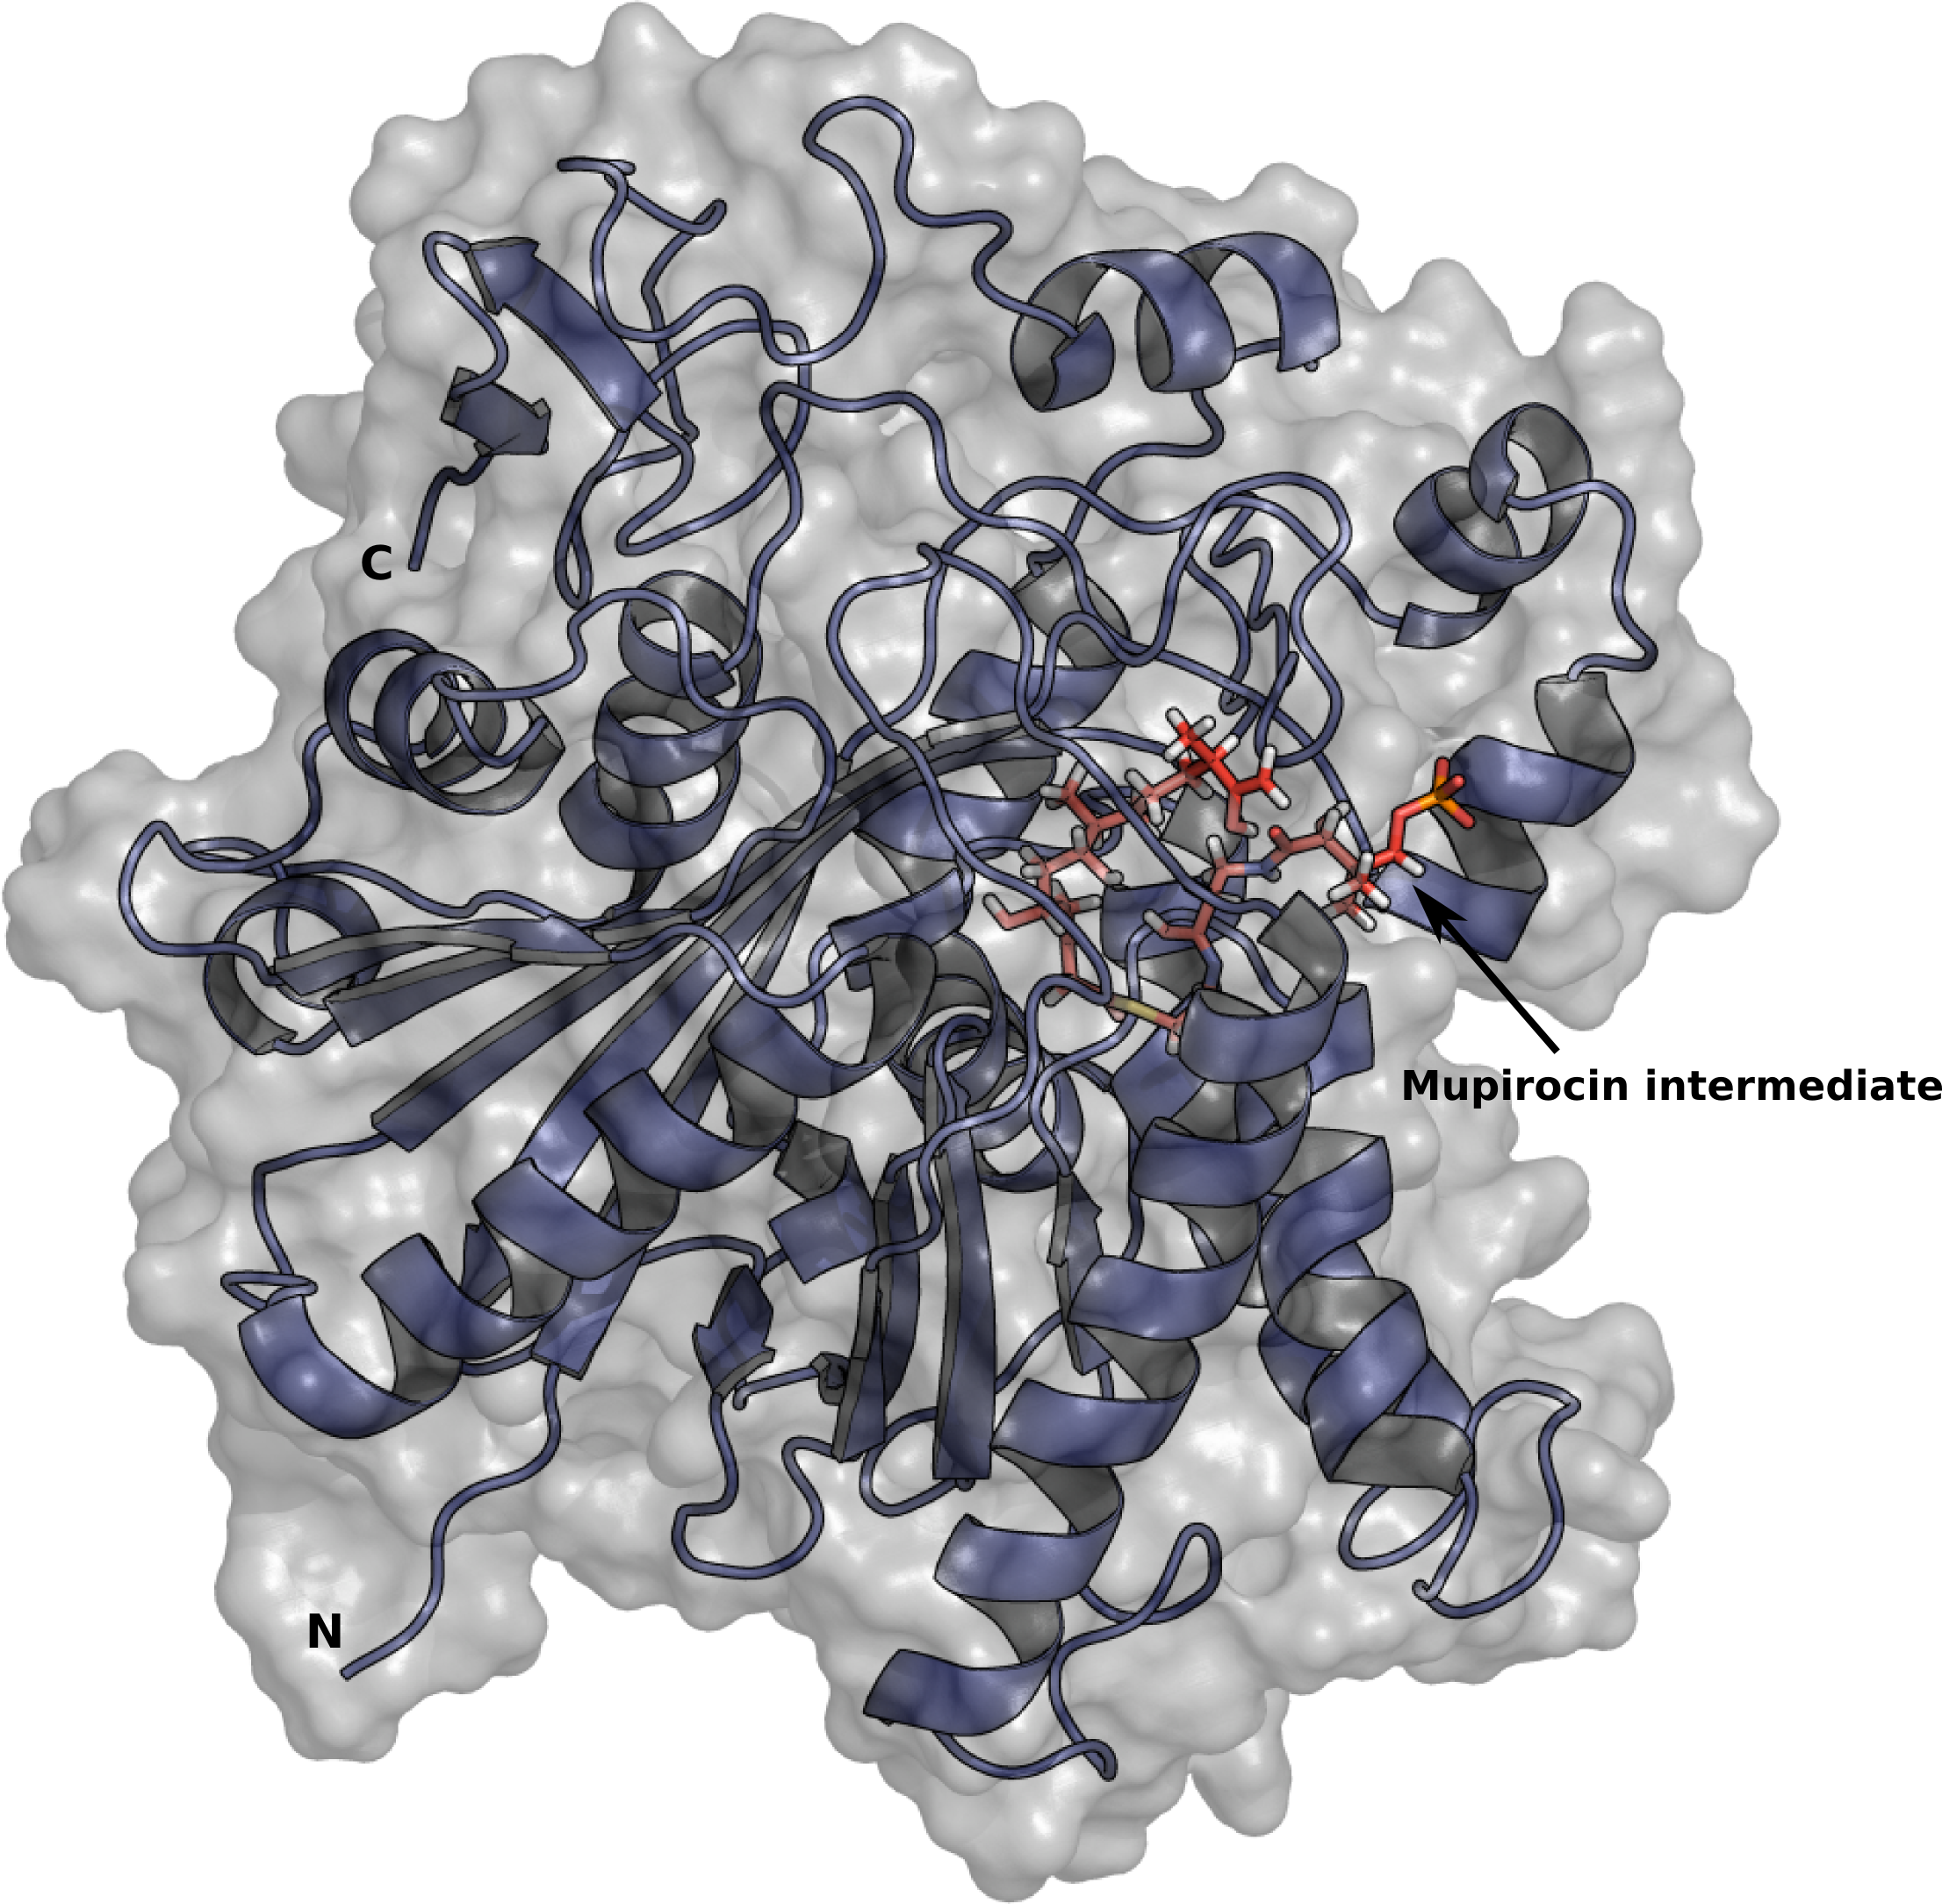
\includegraphics[width=0.9\textwidth, keepaspectratio=true]{graphics/muph.png}}
			\caption[Homology model of MupH complexed with the mupirocin intermediate.]{Homology model of MupH complexed with the mupirocin intermediate based on the HMG-CoA synthase X-ray structure from \textit{Enterococcus faecalis} (PDB ID 1X9E).}
			\label{fig:MupH}
			\end{figure}	

			\setlength\fboxsep{5pt}
			\setlength\fboxrule{1.5pt}
			\begin{figure}[]
			\centering
			\fbox{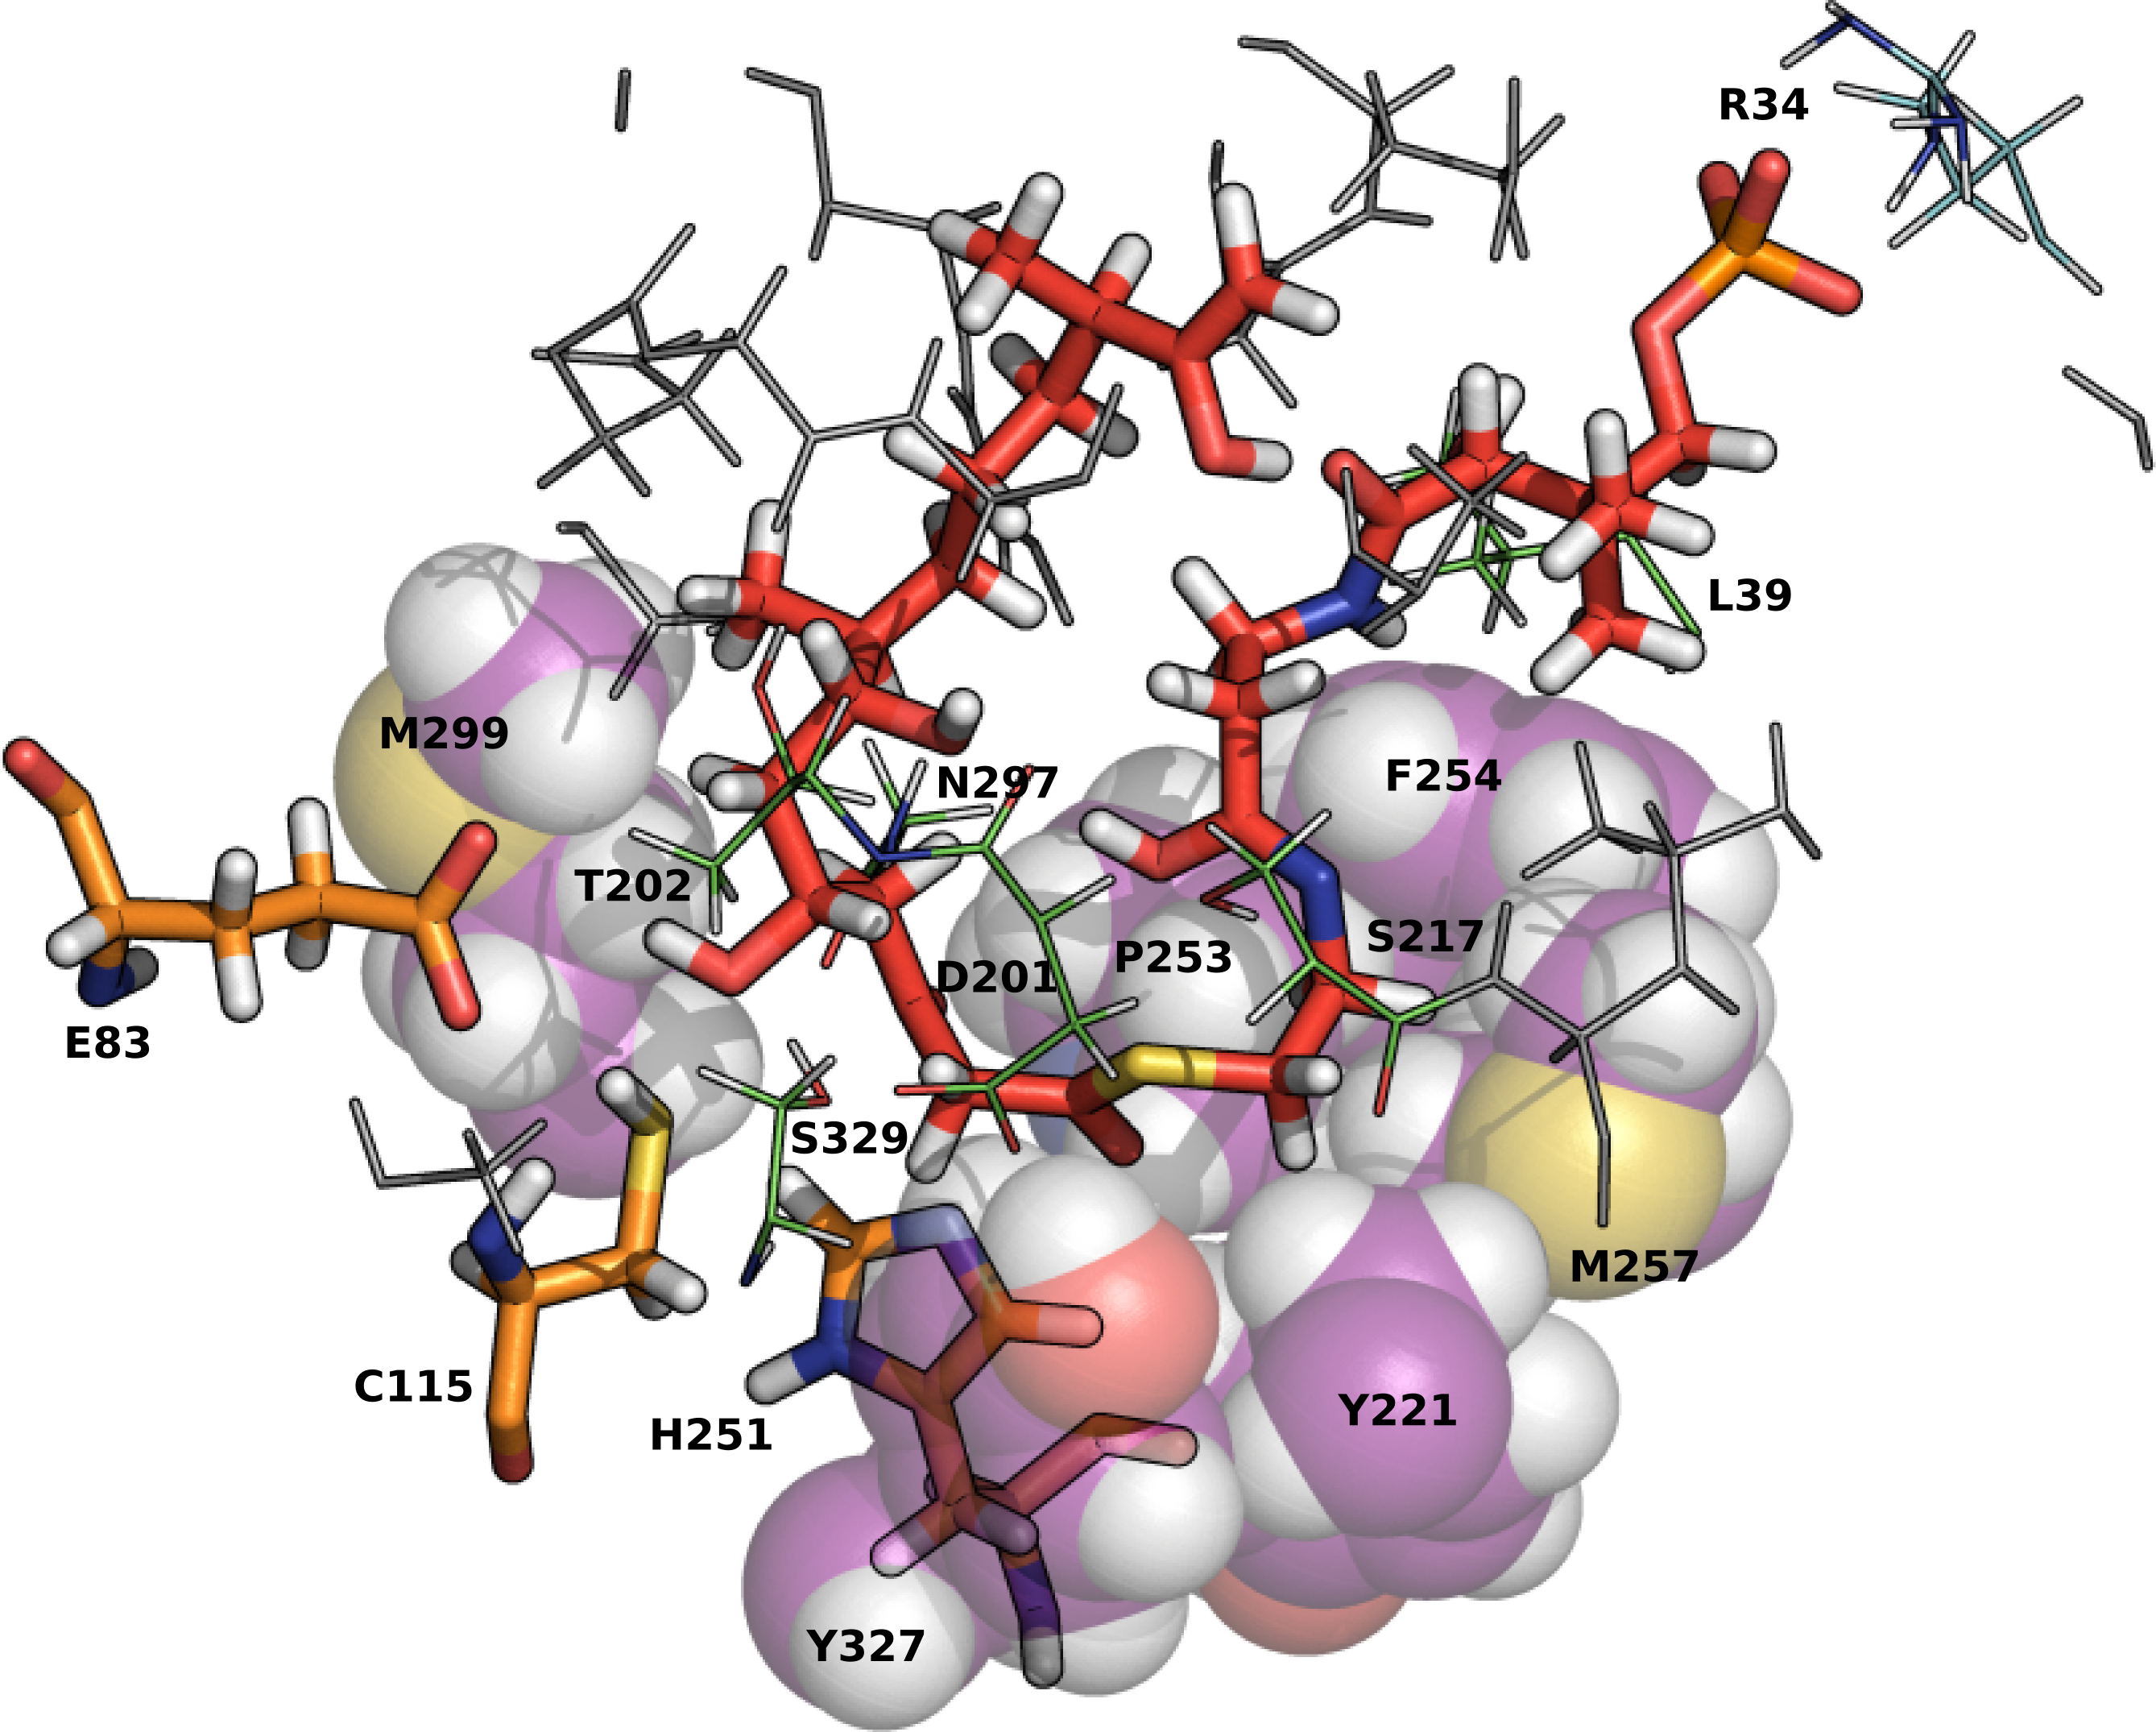
\includegraphics[width=0.9\textwidth, keepaspectratio=true]{graphics/5around.png}}
			\caption[Residues within a 5 \AA{} radius of the mupirocin intermediate.]{Residues within a 5 \AA{} radius of the mupirocin  intermediate. The residues of the catalytic triad are shown as sticks, other active site essential residues are shown as lines with green backbone, tunnel lining residues are shown as spheres, the gate keeper residues are shown as line with cyan backbone. The term catalytic triad, other essential residues, tunnel lining residues and the gate keeper residues are further discussed in detail in the Section \ref{sec:MupHandHomologue}. C115 and E83 are placed close the \bet-carbon thus the model is consistent with the catalytic activity.}
			\label{fig:5around}
			\end{figure}	
				
			\setlength\fboxsep{5pt}
			\setlength\fboxrule{1.5pt}
			\begin{sidewaysfigure}[]
			\centering
			\fbox{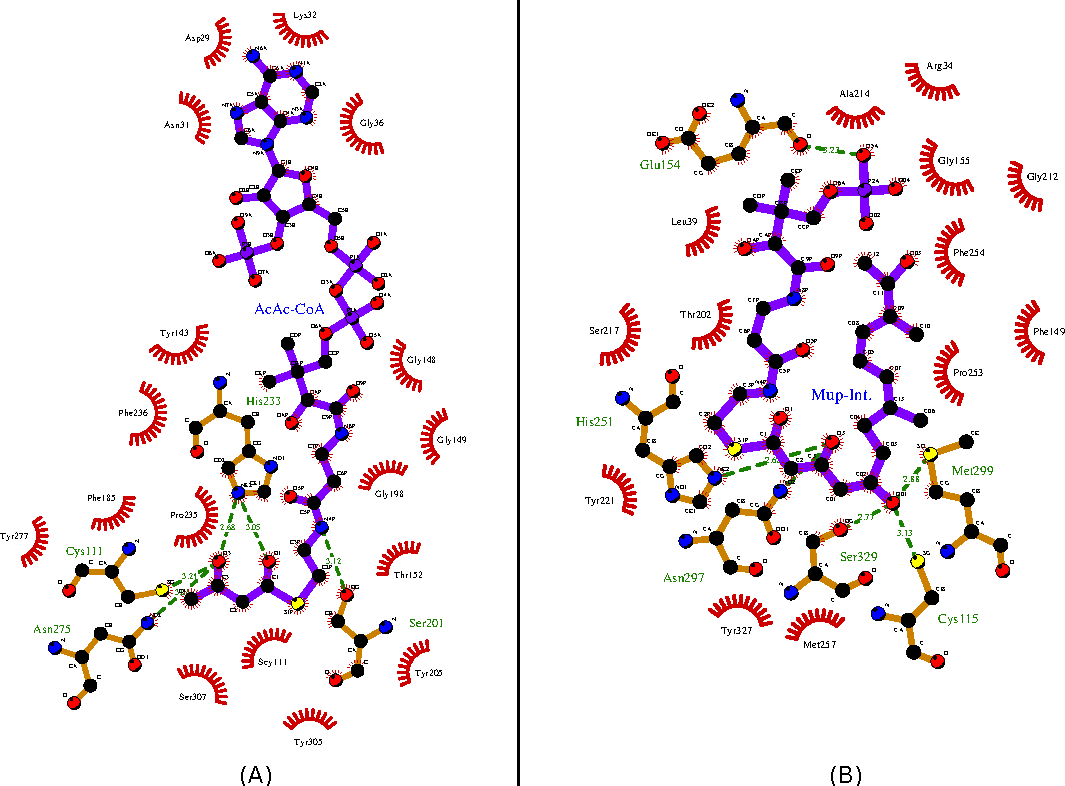
\includegraphics[width=0.8\textwidth, keepaspectratio=true]{graphics/1XPKvsMupH.pdf}}
			\caption[Protein-ligand interaction plot for HMG-CoA homologues.]{Protein-ligand interaction plot for HMG-CoA homologues. (A) crystal structure of \textit{Staphylococuccous aureus} HMG-CoA (PDB ID 1XPK) complexed with acetoacetyl-CoA and (B) modelled MupH complexed with PKS bound mupirocin intermediate. Green dotted lines shows hydrogen bonds and red arches around the residues shows hydrophobic interactions. Plot produced by LigPlot \parencite{Wallace1995}.}
			\label{fig:1XPKvsMupH}
			\end{sidewaysfigure}				
	
	\subsection{Similarity between MupH and HMG-CoA homologues in sequence and structure}
	\label{sec:MupHandHomologue}
	Despite the low level of sequence identity among MupH homologues, the key catalytic and substrate binding residues mentioned in the literature are highly conserved (Figure \ref{fig:MuphModAli}). Residues that are conserved and  identified as important in the literature are listed in Table \ref{tab:MupHconserved_residue}. The conserved residues can be divided into four categories, (1) catalytic triad (2) residues responsible for substrate orientation in the active site (3) tunnel residues (4) gate Keeper residues \parencite{Misra1996, Bahnson2004,Theisen2004,Steussy2005,  Shafqat2010}.
	
		
			\setlength\fboxsep{5pt}
			\setlength\fboxrule{1.5pt}
			\begin{sidewaysfigure} []
			\centering
			\fbox{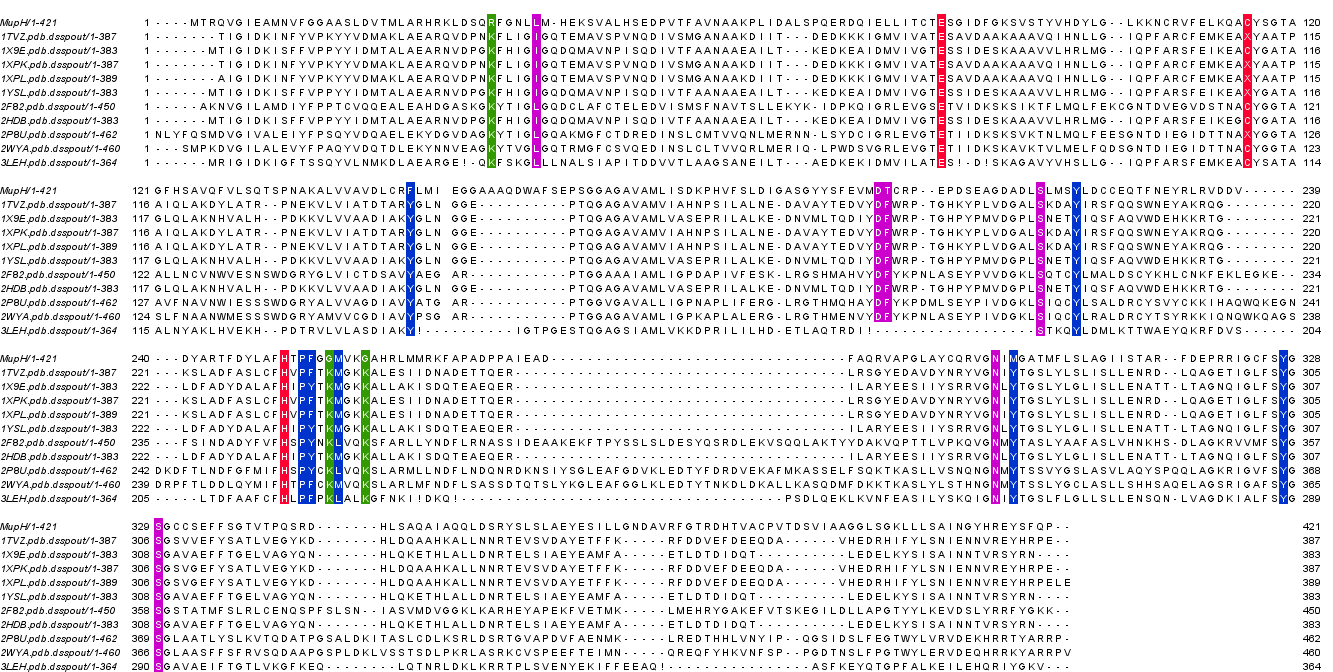
\includegraphics[width=\textwidth, resolution=600, keepaspectratio=true]{graphics/muphmodali.png}}
			%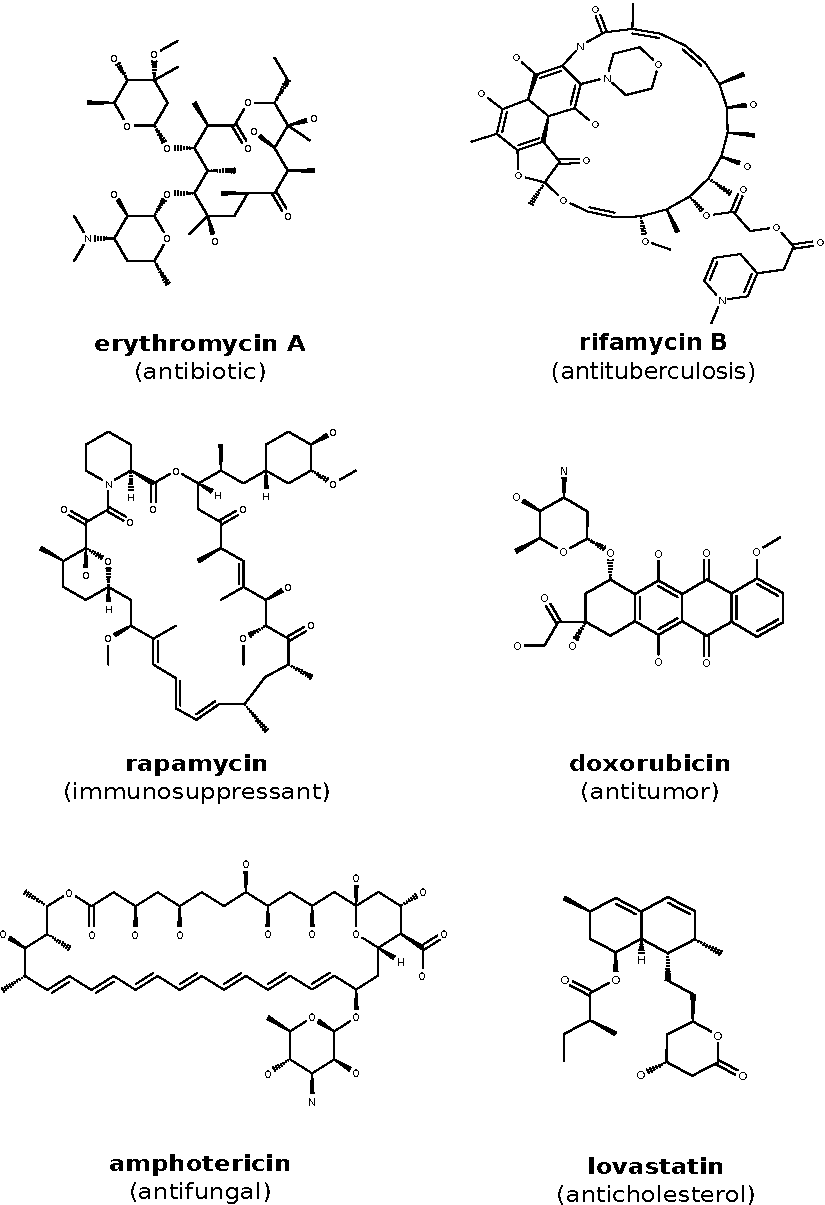
\includegraphics[width=\textwidth, resolution=200, keepaspectratio=true]{graphics/polyketides.png}
			\caption[Sequence alignment of the templates used for the MupH modelling.]{Sequence alignment of the templates used for the MupH modelling. Red: Catalytic Triad, Magenta: residues responsible for the substrate orientation in the active site, Blue: Tunnel residues, Green: Gate keeper residues. Sequences are taken from the template structures ! indicates a break in the chain associated with unresolved residues. }
			\label{fig:MuphModAli}
			\end{sidewaysfigure}
			
				%List of all the residue found conserved in the alignment with annotations from the literature
				\begin{table}[htbp]
				\begin{small}
				\caption{List of all the residues found conserved in the alignment with annotations from the literature}
				\label{tab:MupHconserved_residue}
				\begin{center}
				\begin{threeparttable}[b]
				\begin{tabular}{p{4cm} p{2.5cm} p{2.5cm} p{2.5cm} p{2.5cm} p{2.5cm} }
				\toprule[2pt]
				 & \textit{Homo sapiens} & \textit{Staphylococcus aureus} & \textit{Enterococcus faecalis} & \textit{Pseudomonas fluorescens} \\ 
				 \midrule[1pt]
				MupH orthologue & \multicolumn{1}{c}{} & \multicolumn{1}{c}{} & \multicolumn{1}{c}{} & \multicolumn{1}{c}{x} \\ 
				HMG-CoA orthologue & \multicolumn{1}{c}{x} & \multicolumn{1}{c}{x} & \multicolumn{1}{c}{x} & \multicolumn{1}{c}{} \\ 
				PDB ID & 2WYA & 1XPL, 1XPK & 1X9E, 1YSL & MupH \\ 
				 &  &  &  &  \\ 
				Active Site & GLU 132 & \textbf{GLU 79} & \textbf{GLU 79} & GLU 83 \\ 
				 & CYS 166 & \textbf{CYS 111} & \textbf{CYS 111} & CYS 115 \\ 
				 & HIS 301 & \textbf{HIS 233} & \textbf{HIS 233} & HIS 251 \\ 
				Other essential active site residues & ASN 380 & \textbf{ASN 275} & \textbf{ASN 275} & ASN 297 \\ 
				 & ASP 240 & ASP 184 & \textbf{ASP 184} & ASP 201 \\ 
				 & PHE 241 & PHE 185 & \textbf{PHE 185} & THR 202 \\ 
				 & SER 258 & SER 201 & SER 201 & SER 217 \\ 
				 & SER 414 & \textbf{SER 307} & \textbf{SER 308} & SER 329 \\ 
				 & LEU 88 & ILE 37 & ILE 37 & LEU 39 \\
				Tunnel Residues & TYR 200 & TYR 143 & \textbf{TYR 143} & PHE 149 \\ 
				 & TYR 262 & TYR 205 & TYR 205 & TYR 221 \\ 
				 & PHE 304 & PHE 236 & TYR 236 & PHE 254 \\ 
				 & TYR 382 & TYR 277 & TYR 277 & MET 299 \\ 
				 & TYR 412 & TYR 305 & TYR 306 & TYR 327 \\ 
				 & PRO 303 & PRO 235 & PRO 235 & PRO 253 \\ 
				 & MET 307 & MET 239 & MET 239 & MET 257 \\ 
				Gate Keeper Residues & LYS 83 & LYS 32 & LYS 32 & ARG 34 \\ 
				 & LYS 266 & LYS 238 & LYS 238 & GLY 256 \\ 
				 & LYS 310 & LYS 242 & LYS 242 & GLY 260 \\ 
				\bottomrule[2pt]
				\end{tabular}
				\begin{tablenotes}
					\item[*] Residues highlighted in bold are conserved and identified as important in the literature \parencite{Theisen2004, Steussy2005, Shafqat2010}. The non-bold residues are from the alignment
					\end{tablenotes}
				\end{threeparttable}
				\end{center}
				\end{small}
				\end{table}
	
		\subsubsection{Catalytic triad and the essential residues responsible for substrate orientation in the active site}
		\label{sec:catalytictriad}
		In the sequence and structure comparison of all the HMG-CoA homologue structures from \textit{Staphylococcus auereus, Enterococcus faecalis} and \textit{Homo sapiens} used in this study and MupH, the \textbf{catalytic triad} (Cys - His - Glu) is found to be conserved. The residues in the active site responsible for the correct orientation of the substrate are also absolutely conserved with some minor variation in MupH.
		
		The acetyl moiety bound to the catalytic cysteine (Figure \ref{fig:muphreact}) is constrained by interactions with  Tyr 143, Phe 185, His 233, Asn 275, Ser 307 (\textit{Staphylococcus aureus}, PDB ID 1XPK). Tyr 143 and Phe 185 residues are in hydrophobic contacts with the ligand as depicted in Figure \ref{fig:1XPKvsMupH}(A). In the MupH these residues are mutated to Phe 149 and Thr 202 respectively, however they are still in contact (Figure \ref{fig:1XPKvsMupH}(B)). The others are conserved, which may help to constrain the acetyl moiety and the rest of the substrate in the PKS bound intermediate. It was hypothesised that the orientation of the acetylated cysteine  in the \textit{Staphylococcus auereus} (PDB ID 1XPK) HMG-CoA synthase structure helps to form a hydrogen bond between the backbone amide of Ser 307 and the carbonyl oxygen of the thioester for stabilizing the oxyanion formed during the transfer of acetyl to the catalytic cysteine (Figure \ref{fig:HMGCO-Areact}) \parencite{Theisen2004}. In MupH this Ser 329 is also conserved which suggests a similar role.

		The HMG moiety of HMG-CoA occupies the catalytic pocket such that its \bet-hydroxyl group hydrogen bonds to His 301 as in Human HMG-CoA synthase structure (PDB ID 2WYA) and Asn 380 while the terminal carboxyl interacts with Glu 132 and the backbone amide of Ser 414 \parencite{Shafqat2010}. In Figure \ref{fig:1XPKvsMupH}(B), MupH His 251 and Asn 297 can be seen forming hydrogen bonds with the \bet-hydroxyl group of the ligand. However, since there is no terminal carboxyl in the mupirocin intermediate close to the corresponding Glu and Ser there is no interaction found.
		
		\subsubsection{Tunnel residues}
		\label{sec:tunnelresidues}
		A set of hydrophobic residues populates the middle portion of the active site \textbf{tunnel} forming a hydrophobic lining. No direct hydrogen bonds are made between the enzyme and the CoA as it passes through this hydrophobic sleeve. MupH is also found to have similar residues (Figure \ref{fig:MuphModAli}) and the homology model indicates a hydrophobic interaction with the ligand along the tunnel sleeve (Figure \ref{fig:1XPKvsMupH}(A)). These residues seem to interact with the phosphopantetheine arm of the CoA specifically, as the gate keeper residues are responsible for stabilizing the nucleotide moiety in the CoA. In avian HMG-Coa synthase, several of these residues have been mutated to leucine with only modest changes in enzyme kinetics. 
		
		\subsubsection{Gate keeper residues}
		\label{sec:gatekeeperresidues}
		In the standard HMG-CoA enzymes, the solvent exposed outer edge of the active site tunnel is populated by a number of basic residues, Lys 32, Lys 238, Lys 242 (PDB ID 1X9E), which hydrogen bond with ribose phosphate from the CoA moiety but not the phosphopantetheine moiety. These residues are not found to be conserved in MupH as shown in the alignment (Figure \ref{fig:MuphModAli}). This variation in the gate keeper residues may be because the likely substrate of MupH, unbranched monic acid is directly attached to the catalytic serine of the ACP via the phosphopantetheine arm and lacks the nucleotide moiety and associated phosphates that are found in CoA.
		
		Figure \ref{fig:MuphOrthoAli} represents the sequence alignment between the MupH orthologs as found by PSI -blast search against the NCBI's protein database for sequences with sequence similarity above 60\% and with keyword “polyketide” in the query, to make sure that the sequences are true MupH orthologs. The alignment highlights all the key conserved residues as found in the alignment of HMG-CoA orthologs. The alignment also highlights the conservation of the residues among the MupH orthologs which are found to be mutated in the HMG-CoA ortholog alignment.
		
			\setlength\fboxsep{5pt}
			\setlength\fboxrule{1.5pt}
			\begin{sidewaysfigure} []
			\centering
			\fbox{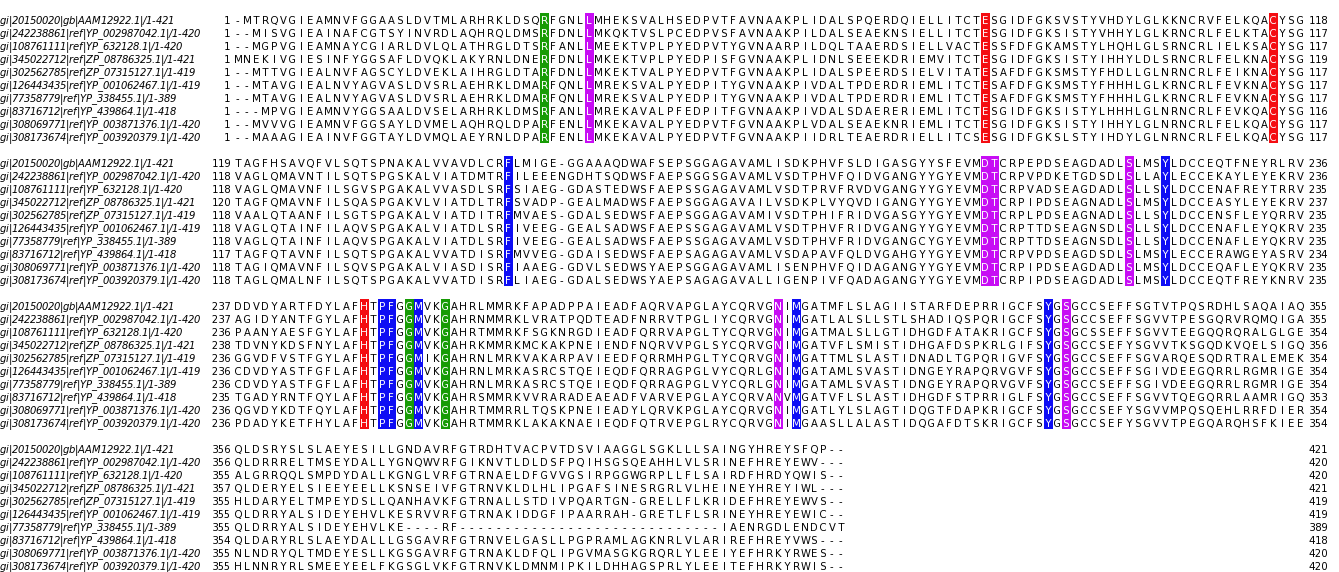
\includegraphics[width=\textwidth, resolution=600, keepaspectratio=true]{graphics/muph_homolog_ali.png}}
			%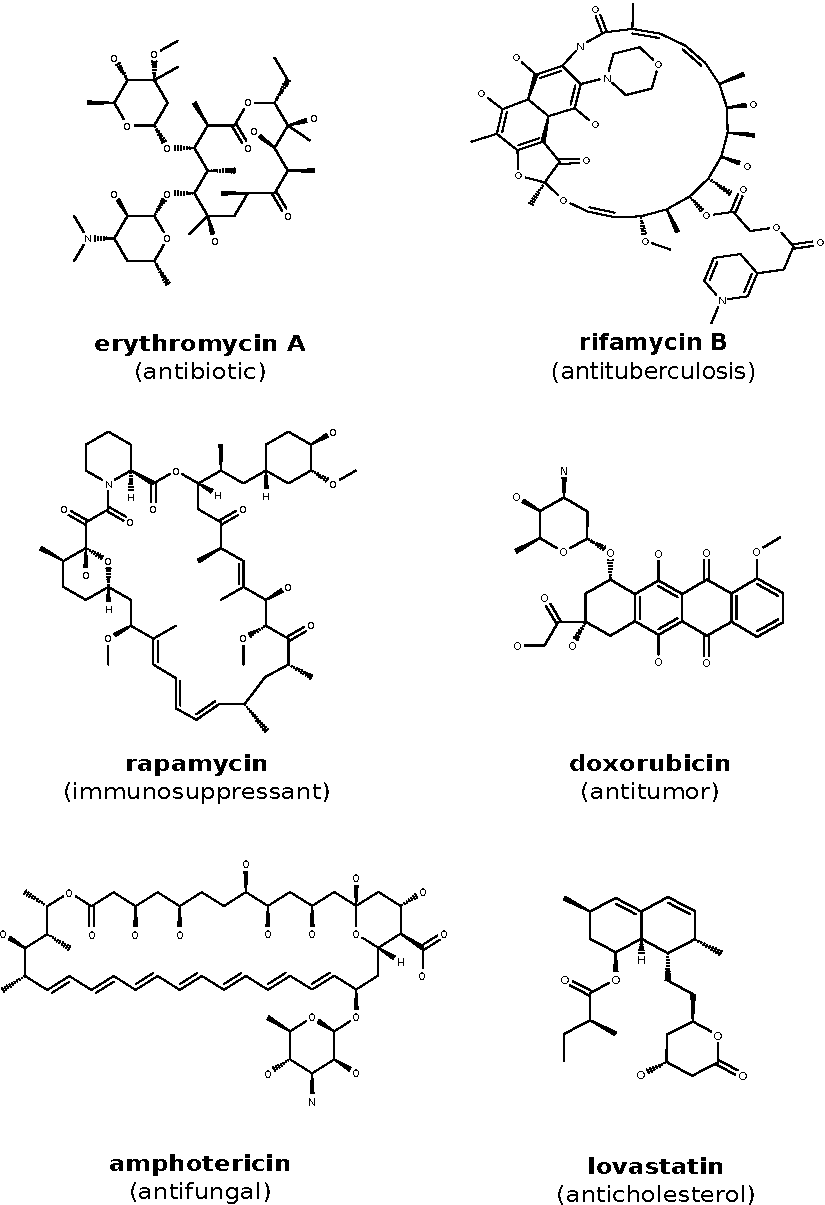
\includegraphics[width=\textwidth, resolution=200, keepaspectratio=true]{graphics/polyketides.png}
			\caption[Sequence alignment of the MupH orthologs.]{Sequence alignment of the MupH orthologs. Red: Catalytic triad, Magenta: residues responsible for the substrate orientation in the active site, Blue: Tunnel residues and Green: Gate keeper residues. }
			\label{fig:MuphOrthoAli}
			\end{sidewaysfigure}				
\newpage

	\subsection{Proposed MupH reaction mechanism}
	\label{sec:muphreact}
	The similarities between the sequence and structure of HMG-CoA synthase and MupH, and the conservation of key catalytic residues, may suggest a similar reaction mechanism for both enzymes. The acetyl moiety attached to mAacpC condenses with the \bet-ketothioester moiety bound to PKS (i.e. mACP3a and mACP3b). In the proposed mechanism, MupH His 251 (catalytic base) seems to attack catalytic Cys 115 which in turn would attack the carbonyl carbon of Ac-mAcpC, thereby transferring the acetyl group to the Cys-S atom and releasing the mAcpC-SH.		
	
	In the second step, the methyl group of acetylated-Cys is deprotonated by the general base Glu 83 to form a carbanion which attacks the \bet-carbonyl of the incoming thioester moiety of ACP-mupA3a/b bound intermediate (second substrate), followed by the condensation of Ac-S-Cys and \bet-ketothioester moiety of the PKS bound intermediate, which forms an enzyme:glutaryl thioester. Ser 329 seems to play a primary role in the formation of an oxyanion hole that stabilises the tetrahedral intermediate in this reaction \parencite{Wu2007}. The resultant enzyme:glutaryl thioester is hydrolysed to release the product glutaryl thioester and regenerate the reduced cysteine. Glu 83 mediates the hydrolysis step.
	
	The glutaryl thiolester is dehydrated by MupJ thus producing glutaconate intermediate, which on MupK mediated decarboxylation gives the 3-methylbut-2-enoyl thioester moiety in monic acid precursor (Figure \ref{fig:muphreact}).
	
			\setlength\fboxsep{5pt}
			\setlength\fboxrule{1.5pt}
			\begin{sidewaysfigure} [!]
			\centering
			\fbox{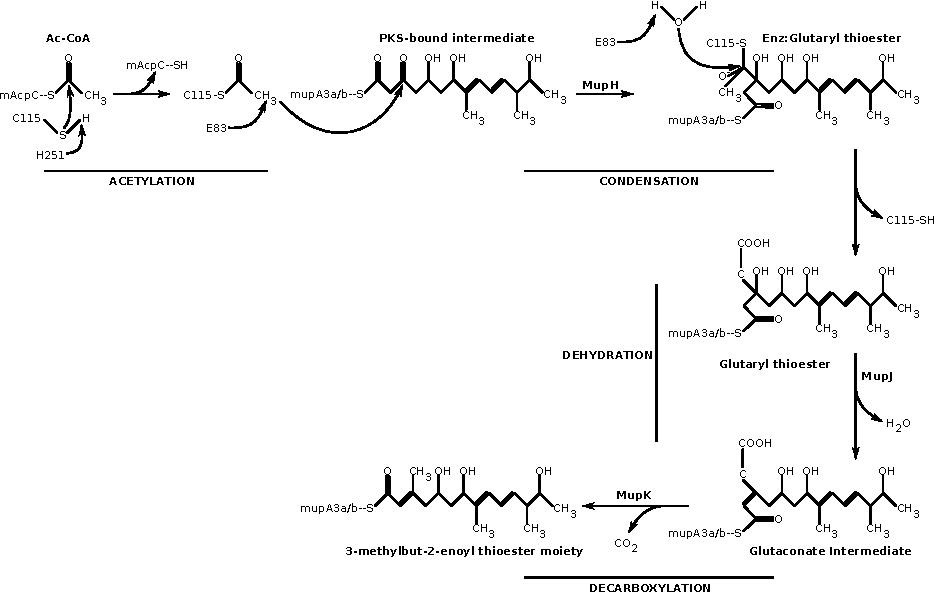
\includegraphics[width=0.9\textwidth, keepaspectratio=true]{graphics/muphreact.pdf}}
			\caption[Proposed reaction mechanism of MupH in the HCS cassette.]{Proposed reaction mechanism of MupH in the HCS cassette.}
			\label{fig:muphreact}
			\end{sidewaysfigure}					

\newpage
			
	\subsection{MupH and ACP (mupA3a and mupA3b) interaction}
	\label{sec:MupHACPInteraction}
	The modelled MupH and the NMR determined ACP structures were docked to predict the probable interaction between them. The HADDOCK \parencite{DeVries2010} program was used to carry out the docking analysis in two different ways (as described in Section \ref{sec:acpMuphDocking}). In the first method HADDOCK utilizes a set of active and passive residues in which it aims to maximise the interaction of each active residue with as many of the atoms of all passive and active residues as possible. Active residues should have a high degree of evidence that they are at the interface of the complex, e.g. residues with high chemical shift perturbation during NMR titration. Passive residues are typically residues with weaker evidence of involvement in the interface, or surface exposed residues neighbouring the active residues. The definitions thus make no presupposition that an interaction will occur and the system of ambiguous interaction restraints (AIR) is used to optimise the interaction of the active residues with all other residues (see Section \ref{sec:Docking} for details).
	
	The active residues were the catalytic serine (Ser 38) of ACP-mupA3a and Arg34, Leu 39, Glu 154 and Ala 214 of MupH, these residues were chosen based on the expected position in the MupH acive site tunnel opening of the phosphopantetheine, which must be covalently bound to serine of ACP-mupA3a. Passive residues were residue contiguous with the active residues and predicted by the program PIER as being part of the interacting interface (Table \ref{tab: active_and_passive}) . PIER uses the physicochemical properties of the atomic groups at the protein surface. Here all the residues for the ACP-mupA3a and MupH which had a PIER Value of 30 or above were defined as interface residues. Figure  \ref{fig:activepassive} shows the docked state of MupH and ACP-mupA3a along with the ligand inside the active site of MupH.
	
	\begin{table}[htbp]
	\begin{small}
	\caption{Interface residues as predicted by PIER and used in HADDOCK as Active and Passive residues.}
	\label{tab: active_and_passive}	
	\begin{center}
	\begin{tabular}{p{7.5cm} p{7.5cm}}
	\toprule[2pt]
	\multicolumn{1}{c}{\textbf{ACP}} & \multicolumn{1}{c}{\textbf{MupH}} \\ 
	\midrule[1pt]
	\textbf{Active} & \textbf{Active} \\ 
	\multicolumn{1}{l}{SER 38} & ARG 34, LEU 39, GLU 154, ALA 214 \\
	\textbf{Passive} & \textbf{Passive} \\ 
	ALA 15, MET 17, LEU 18, TYR 19, ILE 40, TYR 62, THR 63 & LEU 30, PHE 35, LEU 38, GLY 153, GLY 155, GLY 156, SER 168, GLY 212, ASP 213, ASP 215, SER 217, LEU 218, PHE 254, MET 257 \\ 
	\bottomrule[2pt]
	\end{tabular}
	\end{center}
	\end{small}
	\end{table}

			\setlength\fboxsep{5pt}
			\setlength\fboxrule{1.5pt}
			\begin{figure} [h!]
			\centering
			\fbox{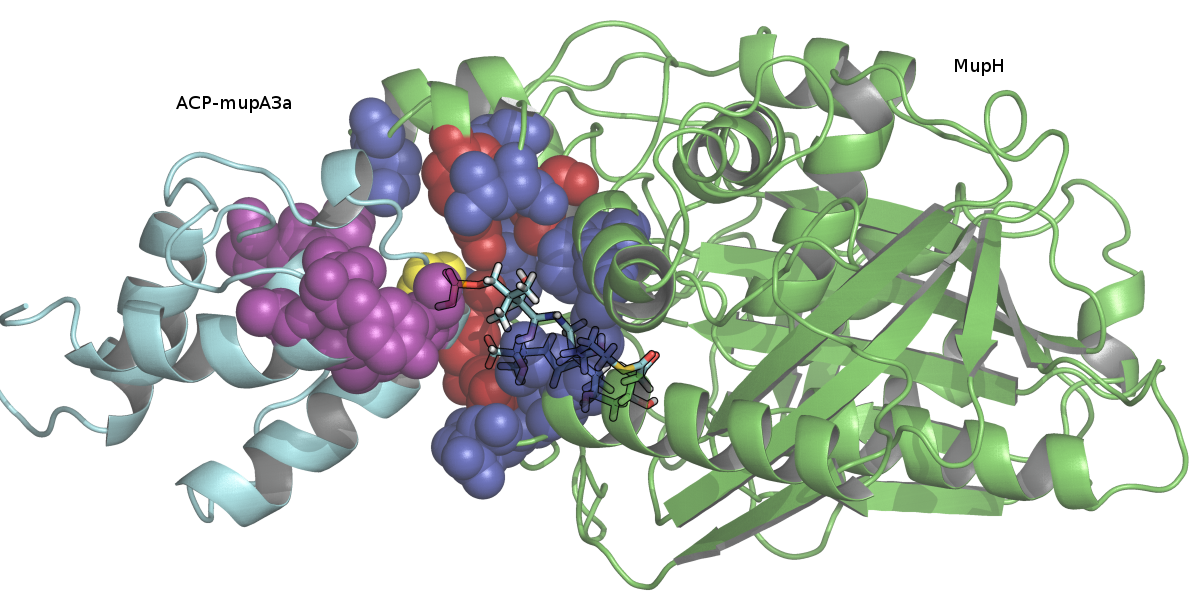
\includegraphics[width=0.9\textwidth, keepaspectratio=true]{graphics/activepassive.png}}
			\caption[The ACP-MupH complex structure predicted by HADDOCK.]{The ACP (cyan) - MupH (green) complex structure predicted by HADDOCK. Yellow: active residue on ACP, Purple: passive residues on ACP, Red: active residues on MupH and Blue: passive reisudes on MupH . The ligand (sticks) shows the location and probable orientation of the phosphopantetheine + mupirocin intermediate in the active site.}
			\label{fig:activepassive}
			\end{figure}					

	In the second method the docking of each of the ACP-mupA3a and ACP-mupA3b with the MupH ligand complex was carried out using the HADDOCK webserver with a  distance restraint of 2.0 \AA{} between the phosphorous of phosphopantetheine bound in the active site of MupH and the OG of the serine (S38/142) residue of ACP-mupA3a or mupA3b. To anchor the ligand in the active site, an additional restraint of 9.13 \AA{} was placed between the sulphur of the thioester linkage in the ligand and the C$ \alpha $ of the catalytic Cysteine (C115) of MupH. HADDOCK produced a single cluster for ACP-mupA3a and 3 clusters for ACP-mupA3b, each cluster represented by four complexes.

		\subsubsection{Interface analysis}
		\label{sec:InterfaceAnalysis}
		The residues at the interface of the ACP and MupH docked complex using distance restraints were determined using a PyMol script (\url{http://www.pymolwiki.org/}) (Table \ref{tab: interface_res}). The interacting pairs of residues between ACP-mupA3a/b and MupH were determined using the CONTAC module of WHATIF \parencite{Vriend1990} (Table \ref{tab: interacting_pairs}). Two of the ACP-mupA3b clusters mimic the binding seen in the ACP-mupA3a:MupH complex, whilst the other ACP ACP-mupA3b cluster binds to MupH at the opposite side of the active site entrance (a rotation of approximately 180 degrees around the ligand bind site, see figure \ref{fig:180opps}). Despite this variation, the residues Ser 38/142, Val 39/143, Asp 59/163, Tyr 62/166, Thr 63/167 of ACPs ACP-mupA3a/mupA3b were found at the interface of all 16 complexes, the latter three residues being on the surface of Helix III, and S38 being the active site serine. A representative complex is shown in figure \ref{fig:repcomplex} with an emphasis on helix III residues and their corresponding interacting residues Arg 34, Met 257 and Arg 263 on MupH. The central position of helix III of the ACPs in the complex, higher levels of conservation around this helix, and its shifted orientation compared to other ACPs all point to it being critical to the recognition of the ACPs by MupH and its orthologues.
		
			\setlength\fboxsep{5pt}
			\setlength\fboxrule{1.5pt}
			\begin{figure} [h!]
			\centering
			\fbox{\includegraphics[width=0.9\textwidth, keepaspectratio=true]{graphics/180opps.pdf}}
			\caption[The representative complex of MupH:ACP-mupA3b.]{The representative complex of MupH:ACP-mupA3b. The representative complex of MupH:ACP-mupA3b from the cluster 1 (green) with the representative complex from cluster 2 superposed (cyan). The cluster 2 representative is similar in position to the binding orientation of cluster 3 and cluster 4 of MupH:ACP-mupA3b and of the representative cluster of MupH:ACP-mupA3a. The docked states of ACP-mupA3b in cluster 1 are almost 180 degrees rotated around the ligand binding pocket of MupH compared to the other clusters.}
			\label{fig:180opps}
			\end{figure}				
			
			\setlength\fboxsep{5pt}
			\setlength\fboxrule{1.5pt}
			\begin{figure} [h!]
			\centering
			\fbox{\includegraphics[width=0.9\textwidth, keepaspectratio=true]{graphics/repcomplex.pdf}}
			\caption[A representative complex with ACP-mupA3a.]{A representative complex with ACP-mupA3a. A representative complex with ACP-mupA3a (red), polyketide intermediate bound to S38 in ACP (spheres) and MupH (blue) showing interface residues on ACP V39, D59, Y62 and T63 and their interacting partners R34, M257 and R263 on MupH. C115, H251and E83 are the catalytic triad in MupH.}
			\label{fig:repcomplex}
			\end{figure}				

			\begin{table}
			\begin{small}
			\caption{List of residues found at the interface of the predicted ACP-mupA3a:MupH complexes and of predicted ACP-mupA3b:MupH complexes}
			\label{tab: interface_res} 
			\begin{center}
			\begin{threeparttable}[b]
			\begin{tabular}{p{2cm} p{2cm} p{3.25cm} p{3.25cm} p{3.25cm}} \\
			\toprule[2pt]
			\multicolumn{ 2}{p{4cm}}{MupH (total 16 complexes, 4 with ACP-mupA3a and 12 with ACP-mupA3b)} & Residues in ACP-mupA3a that are found in cluster 1 of ACP-mupA3b:MupH complexes & Residues in ACP-mupA3b that are found in clusters¶ 2 and 3 of ACP-mupA3b:MupH complexes \tnote{a} & Residues in ACP-mupA3b that are found in cluster 1 of ACP-mupA3b:MupH complexes \tnote{b} \\ 
			\cmidrule[1pt]{1-2}
			\textit{Residue} & \multicolumn{1}{c}{\textit{Frequency}} &  &  &  \\
			\midrule[1pt]
			ARG 34 & 16 & ARG 30 & PHE 135 & GLY 139 \\
			LEU 38 & 16 & LEU 32 & GLY 139 & MET 140 \\ 
			LEU 30 & 15 & \textbf{SER 38} & \textbf{SER 142} & \textbf{SER 142} \\ 
			ALA 214 & 15 & \textbf{VAL 39} & \textbf{VAL 143} & \textbf{VAL 143} \\ 
			ARG 263 & 15 & ALA 42 & \textbf{ASP 163} & \textbf{ASP 163} \\ 
			ASP 31 & 14 & ARG 46 & \textbf{TYR 166} & ILE 165 \\ 
			GLN 33 & 14 & ALA 58 & \textbf{THR 167} & \textbf{TYR 166} \\
			ASP 215 & 13 & \textbf{ASP 59} &  & \textbf{THR 167} \\ 
			ASN 37 & 12 & \textbf{TYR 62} &  & PRO 169 \\ 
			MET 219 & 12 & \textbf{THR 63} &  &  \\
			LEU 218 & 11 & TYR 64 &  &  \\ 
			GLY 256 & 10 & PRO 65 &  &  \\ 
			GLY 154 & 9 & TRP 73 &  &  \\ 
			GLY 260 & 9 &  &  &  \\
			ARG 267 & 9 &  &  &  \\ 
			LEU 222 & 6 &  &  &  \\ 
			MET 257 & 6 &  &  &  \\ 
			GLY 153 & 5 &  &  &  \\ 
			ILE 152 & 4 &  &  &  \\ 
			\bottomrule[2pt]
			\end{tabular}
			\begin{tablenotes}
			\item[a] Residues in common with the interface of the predicted complexes of the ACP-mupA3b:MupH in cluster 1, 2 and 3 and the ACP-mupA3a:MupH cluster are highlighted in bold. In addition all ACP-mupA3b clusters have G139 at the interface.
			\item[b] Each cluster is comprised of 4 complexes, ACP-mupA3b clusters 2 and 3 bind MupH in a similar orientation to ACP-mupA3a, ACP-mupA3b cluster 1 is rotated through ~180 degrees around the phosphopantetheine with respect to the other clusters.
			\end{tablenotes}
			\end{threeparttable}
			\end{center}
			\end{small}
		    \end{table}
    	
			%List of interacting pairs in mupA3a and mupA3b with MupH.
			\begin{sidewaystable}
			\begin{small}
			\caption{List of interacting pairs in ACP-mupA3a and ACP-mupA3b with MupH.}
			\label{tab: interacting_pairs}
			\begin{center}
			\begin{threeparttable}[b]
			\begin{tabular}{l l l l l l l l l l}
			\toprule[2pt]
			\multicolumn{ 1}{p{1cm}}{MupH residues} & \multicolumn{ 1}{p{1cm}}{mupA3a residues} & \multicolumn{1}{p{2cm}}{mupA3b equivalent} & \multicolumn{1}{p{2cm}}{Frequency (Max. 4)} & \multicolumn{ 1}{p{1cm}}{MupH residues} & \multicolumn{ 1}{p{3cm}}{mupA3b residues clusters 2 and 3} & \multicolumn{1}{p{2cm}}{Frequency (Max. 8)} & \multicolumn{1}{p{1cm}}{MupH residues} & \multicolumn{1}{p{3cm}}{mupA3b residues cluster 1} & \multicolumn{1}{p{2cm}}{Frequency (Max. 4)} \\ 
			\midrule[1pt]
			\underline{GLN 33} & \underline{ARG 46} & \underline{ARG 150} & 4 & \underline{ARG 263} & \underline{ASP 163} & 8 & ARG 34 & GLY 139 & 4 \\ 
			\underline{ARG 34} & \underline{SER 38} & \underline{SER 142} & 4 & \underline{ARG 34} & \underline{VAL 143} & 7 & \textbf{ARG 34} & \textbf{SER 142} & 4 \\ 
			ASP 215 & ARG 30 & GLN 134 & 4 & ALA 214 & GLY 139 & 7 & LYS 29 & THR 167 & 3 \\ 
			ASP 215 & LEU 32 & LEU 136 & 4 & \underline{GLN 33} & \underline{ARG 150} & 6 & GLN 33 & PHE 135 & 3 \\ 
			\underline{MET 257} & \underline{TYR 62} & \underline{TYR 166} & 4 & \underline{ASP 31} & \underline{ARG 150} & 5 & ARG 34 & LEU 138 & 3 \\ 
			LEU 218 & LEU 32 & LEU 136 & 3 & ASP 215 & PHE 135 & 5 & LEU 38 & GLY 139 & 3 \\ 
			GLY 260 & TYR 62 & TYR 166 & 3 & ASN 37 & TYR 166 & 4 & ASP 31 & PHE 135 & 2 \\ 
			\underline{ARG 263} & \underline{ASP 59} & \underline{ASP 163} & 3 & ASP 215 & LEU 136 & 4 & ARG 28 & TYR 166 & 2 \\ 
			\underline{ARG 263} & \underline{THR 63} & \underline{THR 167} & 3 & \underline{\textbf{ARG 34}} & \underline{\textbf{SER 142}} & 3 & LEU 30 & TYR 166 & 2 \\ 
			ARG 267 & TRP 73 & GLU 177 & 3 & \underline{ASN 37} & \underline{ASP 163} & 3 & ARG 34 & TYR 166 & 2 \\ 
			MET 219 & ARG 30 & GLN 134 & 2 & \underline{LEU 38} & \underline{TYR 166} & 2 & LEU 38 & MET 140 & 2 \\ 
			ARG 263 & TYR 62 & TYR 166 & 2 & GLU 154 & MET 140 & 2 & ALA 214 & VAL 143 & 2 \\ 
			ASP 31 & ALA 42 & THR 146 & 1 & ALA 214 & MET 140 & 2 & LYS 29 & PRO 169 & 1 \\ 
			\underline{ASP 31} & \underline{ARG 46} & \underline{ARG 150} & 1 & \underline{LEU 218} & \underline{TYR 166} & 2 &  &  &  \\ 
			\underline{ARG 34} & \underline{VAL 39} & \underline{VAL 143} & 1 & LYS 259 & ASP 163 & 2 &  &  &  \\ 
			\underline{ASN 37} & \underline{ASP 59} & \underline{ASP 163} & 1 & ASP 31 & GLN 147 & 1 &  &  &  \\ 
			LEU 38 & ASP 59 & ASP 163 & 1 & GLN 33 & GLN 147 & 1 &  &  &  \\ 
			\underline{LEU 38} & \underline{TYR 62} & \underline{TYR 166} & 1 & ARG 34 & THR 146 & 1 &  &  &  \\ 
			ASP 215 & GLU 33 & ASP 137 & 1 & ARG 34 & THR 144 & 1 &  &  &  \\ 
			\underline{LEU 218} & \underline{TYR 62} & \underline{TYR 166} & 1 & LEU 38 & VAL 143 & 1 &  &  &  \\ 
			PHE 254 & TYR 62 & TYR 166 & 1 & ASP 215 & GLY 139 & 1 &  &  &  \\ 
			ARG 263 & TRP 73 & GLU 177 & 1 & ASP 215 & TYR 166 & 1 &  &  &  \\ 
			ARG 267 & GLN 77 & ARG 181 & 1 & LEU 216 & PHE 135 & 1 &  &  &  \\ 
			ARG 267 & THR 76 & ARG 180 & 1 & \underline{MET 257} & \underline{TYR 166} & 1 &  &  &  \\ 
			 		&  	     & 		   &   & GLY 260 & ASP 163 & 1 &  &  &  \\ 
			        &        &         &   & \underline{ARG 263} & \underline{THR 167} & 1 &  &  &  \\ 
			\bottomrule[2pt]
			\end{tabular}
				\begin{tablenotes}
				\item[] Residue pairs underlined are found at the interface of at least one ACP-mupA3a:MupH and ACP-mupA3b:MupH (clusters 2 and 3) complexes. Residue pairs in bold are found in both modes of ACP-mupA3b:MupH interaction. 
				\end{tablenotes}
			\end{threeparttable}
			\end{center}
			\end{small}
			\end{sidewaystable}
\newpage			
		\subsubsection{Real value evolutionary trace and PIER analysis}
		\label{sec:RVandPIER}
		It is commonly observed that functionally important residues such as catalytic residues are evolutionary conserved within a protein family. This evolutionary pressure is also seen in the residues which are involved in protein-protein interactions responsible for their function. Therefore, the conservation of the interface residues predicted in the HADDOCK docking experiment was determined using real value evolutionary trace analysis. Real value evolutionary trace analysis \parencite{Lichtarge1996} for ACP-mupA3a/mupA3b and MupH was performed using Evolutionary Trace Viewer \parencite{Morgan2006} (\url{http://mammoth.bcm.tmc.edu/traceview/index.html}). This trace gauges conservation within the context of the phylogenetic tree such that residues that are conserved within a clade but vary between them score highly as do totally conserved residues (details in Section \ref{sec:ET}). The multiple sequence alignment for real value evolutionary trace analysis was carried out using ClustalW with 95 and 75 sequences for ACP-mupA3ab and MupH respectively. Figure \ref{fig:ET} and Figure \ref{fig:etcomplex} show the real value evolutionary trace scores mapped on a representative complex structure of ACP-mupA3a and MupH. The scores are coloured through the spectrum from red to blue, with red indicating predicted importance and blue lack of importance. The ACP is shown as a pink ribbon. The figure shows three views of the same complex; Front View shows the hot (red) patch at the ACP+MupH complex interface. Left view is the clockwise 90 degree rotation from the front view. And the right view is the anti-clockwise 90 degree rotation from the front view. Right View also shows a hot patch at the MupH structure. This hot patch could be a dimer forming interface as the HMG-CoA homologues commonly exit as homodimers, Figure \ref{fig:etcomplex} shows the structure of the HMG-CoA homologue dimer (PDB ID 1X9E) superimposed, on the MupH+ACP complex. The strong evolutionary conserved patch at the interface supports the existence of MupH as a homodimer.

			\setlength\fboxsep{5pt}
			\setlength\fboxrule{1.5pt}
			\begin{figure} [h!]
			\centering
			\fbox{\includegraphics[width=0.9\textwidth, resolution=600, keepaspectratio=true]{graphics/ET.pdf}}
			%\includegraphics[width=\textwidth, resolution=200, keepaspectratio=true]{graphics/polyketides.png}
			\caption[Real value evolutionary trace of MupH homologues.]{Real value evolutionary trace of MupH homologues. The different view shows the functional patch on the predicted interface of MupH. The left view is a 90 degree rotation anticlockwise with respect to the centre, the right view a 90 degree rotation clockwise. Residues on the surface of the MupH are coloured through the spectrum from red to blue, with red indicating predicted importance, blue lack of importance, the ACP is shown as a pink ribbon.}
			\label{fig:ET}
			\end{figure}		

			\setlength\fboxsep{5pt}
			\setlength\fboxrule{1.5pt}
			\begin{figure} [h!]
			\centering
			\fbox{\includegraphics[width=0.9\textwidth, resolution=600, keepaspectratio=true]{graphics/etcomplex.png}}
			%\includegraphics[width=\textwidth, resolution=200, keepaspectratio=true]{graphics/polyketides.png}
			\caption[HmgCoA synthase homo-dimer (grey) from Enterococcous faecalis (PDB accession code 1X9E) superimposed on the MupH:ACP-mupA3a complex 1 from cluster 1.]{HmgCoA synthase homo-dimer (grey) from Enterococcous faecalis (PDB accession code 1X9E) superimposed on the MupH:ACP-mupA3a complex 1 from cluster 1. Residues are coloured by their real value evolutionary trace score, which highlights residues likely to be of functional importance; a rainbow colouring is used from red (most important) to violet (least important). As well as highlighting the ACP:MupH interface, the analysis also highlights some residues on the MupH surface that are distal from the proposed ACP binding site; these are where most HmgCoA synthases form homo dimmers. (Y 62, D 59 and T 63 are identified as being in the top 5.71\%, 22.85\% and 23.80\% respectively of residues for evolutionary importance).}
			\label{fig:etcomplex}
			\end{figure}					
		
		The PIER values calculated in the previous step for MupH were also mapped on the structure and coloured through the spectrum from red to blue, Figure \ref{fig:PIER}(A). It was interesting to see that the residues predicted the important in the real value evolutionary trace analysis also agree with the PIER calculations and similar hot and cold patches can be seen on the surface. However, PIER scores show an additional hot patch on the left view which was not identified in the real value evolutionary trace. For comparison the MupH homologues from kalamanticin (BatC) and thiomarinol (TmlH) clusters were also submitted to PIER analysis Figure \ref{fig:PIER}(B) and (C) respective. The structures of BatC and TmlH were predicted using the same template and alignment as that used for MupH and were superimposed on the MupH+ACP-mupA3a representative complex. These complexes also highlighting similar regions are being important for interface formation, including the additional hot patch of unspecified function. 

			\setlength\fboxsep{5pt}
			\setlength\fboxrule{1.5pt}
			\begin{figure} [!]
			\centering
			\fbox{\includegraphics[width=0.9\textwidth, resolution=600, keepaspectratio=true]{graphics/PIER.pdf}}
			%\includegraphics[width=\textwidth, resolution=200, keepaspectratio=true]{graphics/polyketides.png}
			\caption[PIER analysis of MupH, BatC and TmlH.]{PIER analysis of MupH, BatC and TmlH. The different view shows the functional patch on the predicted interface of (A) MupH, (B) BatC and (C) TmlH. The left view is a 90 degree rotation anticlockwise with respect to the centre, the right view a 90 degree rotation clockwise. Residues on the surface of the MupH are coloured through the spectrum from red to blue, with red indicating predicted importance, blue lack of importance, the ACP is shown as a pink ribbon.}
			\label{fig:PIER}
			\end{figure}

		\subsubsection{Loss of function with Y to F/A mutation in ACP-mupA3a}
		\label{sec:lossoffunc}
		The above mentioned docking results which were also supported by PIER and real value evolutionary trace analysis emphasized on the importance of helix III for the formation of the ACP:MupH interaction. This helix III carried Y62 which was conserved in 95\% of the \bet-branching ACPs and it can be seen pointing towards MupH at the interacting interface and possibly making a favourable methionine to aromatic contact, methionine aromatic interaction were recently reported as important interaction in protein structure \parencite{Valley2012}. M257 was conserved in all the MupH homologue studied except TaF (myxovirescin system). Mutagenesis experiments were carried out by colleagues in Prof. Thomas group to mutate Y62 to F and A in $ \Delta $ACP-mupA3b. Phenylalanine was the most commonly occurring residue at this position in non branching ACPs. Mutating Y62 to F and A lowered the mupirocin production by three to four folds and up to ten folds respectively \parencite{Haines2013}. 
	
	\subsection{BatC complementation failure}
	\label{sec:batccomplement}
	BatC is the MupH equivalent protein from the kalamanticin cluster and it was thought that it should be able to complement MupH and produce the beta-branch in mupirocin. However, the complementation experiments showed that \textit{batC} expressed \textit{in trans} in a $ \Delta $\textit{mupH} strain greatly decreases mupirocin production. Therefore, to answer the question of why BatC did not complement MupH, bioinformatics and molecular modelling analysis was carried out using the previously modelled BatC structure. Assuming that ACP-mupA3a docks to BatC in the same orientation as it docks to MupH, the BatC structure was superimposed on to the ACP-mupA3a+MupH complex and the ACP-mupA3a+BatC model produced was analysed by CONTAC module from WhatIf package. The contacting residues found were conserved and similar to the ACP-mupA3a+MupH complex (Table \ref{tab:batcCONTAC}). 
	
	\begin{table}[htbp]
	\caption{Comparison of the contacting residues in the BatC+ACP-mupA3a pair with the MupH+ACP-mupA3a}
	\begin{center}
	\begin{tabular}{lll}
		\toprule[2pt]
		\multicolumn{1}{l}{\textbf{MupH}} & \multicolumn{1}{l}{\textbf{BatC}} & \multicolumn{1}{l}{\textbf{ACP-mupA3a}} \\ \midrule[1pt]
		R34                                & R33                                & S38                                \\
		D215                               & D214                               & L32                                 \\
		L218                               & L217                               & Y62                                 \\
		L219                               & L218                               & P65                                 \\
		L222                               & L221                               & T63                                 \\
		M257                               & M256                               & Y62                                 \\
		G260                               & G259                               & Y62                                 \\
		R267                               & R266                               & T76                                 \\ \bottomrule[2pt]
	\end{tabular}
	\end{center}
	\label{tab:batcCONTAC}
	\end{table}

	Since the contacting pairs of the residues in the BatC+ACP-mupA3a complex were found to be similar to the MupH+ACP-mupA3a complex in the CONTAC analysis it was thought that it is possible that due to superimposing the BatC structure on the MupH+ACP-mupA3a complex the analysis was biased towards the similar positions. In order to address this issue modelled BatC structure was docked to the ACP-mupA3a using the similar distance restraints as it was used for the MupH+ACP-mupA3a complex. The BatC+ACP-mupA3a docked complex came out to be almost 180 degree flip of the MupH+ACP-mupA3a complex. It was not clear why it happened as the BatC interface when superimposed on MupH+ACP-mupA3a complex was visually similar. However, in the MupH docking to ACP-mupA3b one of the clusters out of the four was similar to the BatC docking therefore, the 180 degree flip orientation was plausible but it was not dominating. In BatC docking all the complexes from both the clusters had the same orientation.  To answer this question it was thought that it might be the electrostatic potentials on the interface which are different for MupH and BatC. The electrostatic potential shows the electrostatic properties on the surface of a molecule in solution. Therefore, for two molecules to interact with each other they should have complementary electrostatic potential. Similar potentials will obviously repel each other. 
	
	To test this hypothesis the APBS \parencite{Baker2001} plugin in PyMol was used in conjunction with PDB2PQR \parencite{Dolinsky2004}. The electrostatic potentials were calculated separately for MupH, BatC and ACP-mupA3a (docked as well as BatC superimposed on MupH+ACP-mupA3a complex) and the structures were superimposed to their respective complexes for comparison. The orientation of the MupH or BatC was kept the same. Three figures were rendered for each of the complex in three different orientations for the solvent accessible and the iso surfaces. The first is the \textquotedblleft front view\textquotedblright, which shows the interacting interface as flat as possible. The other two are in left and right orientation around Y axis. The degree of rotations used were slightly different for MupH and BatC in order to highlight their interesting features as far as possible. 
	
	The electrostatic potentials for both BatC and MupH were found to be very similar with only a few subtle differences. Those few differences might be significant but it was difficult to find any difference in the specificity of MupH and BatC based on the electrostatic potentials on the protein interface. 
	
			\setlength\fboxsep{5pt}
			\setlength\fboxrule{1.5pt}
			\begin{figure} [!]
			\centering
			\fbox{\includegraphics[width=0.9\textwidth, resolution=600, keepaspectratio=true]{graphics/solsurfmuphbatcacp.pdf}}
			%\includegraphics[width=\textwidth, resolution=200, keepaspectratio=true]{graphics/polyketides.png}
			\caption[Electrostatic potential mapped on the solution accessible surface of MupH, BatC and ACP.]{Electrostatic potential mapped on the solution accessible surface of MupH, BatC and ACP. BatC was superimposed on the MupH + ACP-mupA3a complex. The three different orientations (Front, Left and Right ) were made to clearly show the mapped potentials at the interface. The scale at the bottom shows the intensity of the negative (red) and positive (blue) potential.}
			\label{fig:solsurfmuphbatcacp}
			\end{figure}

			\setlength\fboxsep{5pt}
			\setlength\fboxrule{1.5pt}
			\begin{figure} [!]
			\centering
			\fbox{\includegraphics[width=0.9\textwidth, resolution=600, keepaspectratio=true]{graphics/isosurfmuphbatcacp.pdf}}
			%\includegraphics[width=\textwidth, resolution=200, keepaspectratio=true]{graphics/polyketides.png}
			\caption[Electrostatic potential mapped as the iso surface on MupH, BatC and ACP.]{Electrostatic potential mapped as the iso surface on MupH, BatC and ACP. BatC was superimposed on the MupH + ACP-mupA3a complex. The three different orientations (Front, Left and Right ) were made to clearly show the mapped potentials at the interface. The scale at the bottom shows the intensity of the negative (red) and positive (blue) potential.}
			\label{fig:isosurfmuphbatcacp}
			\end{figure}

			\setlength\fboxsep{5pt}
			\setlength\fboxrule{1.5pt}
			\begin{figure} [!]
			\centering
			\fbox{\includegraphics[width=0.8\textwidth, resolution=600, keepaspectratio=true]{graphics/dockedbatcacp.pdf}}
			%\includegraphics[width=\textwidth, resolution=200, keepaspectratio=true]{graphics/polyketides.png}
			\caption[Electrostatic potential mapped on the BatC and ACP-mupA3a docked complex.]{Electrostatic potential mapped on the BatC and ACP-mupA3a docked complex. The orientation of the BatC is kept same as that of the previous figures while the ACP can be seen as docked in almost 180 degree flip orientation. Both the solution accessible surface as well as the iso surface are shown in three different orientations (Front, Left and Right). The scale at the bottom shows the intensity of the negative (red) and positive (blue) potential.}
			\label{fig:dockedbatcacp}
			\end{figure}
		
		\subsubsection{Gain of function with L to M mutation in BatC complementation }
		\label{sec:LtoMBatC}
		The above mentioned docking and electrostatic potential analysis failed to project any striking difference between the interface of MupH with ACP-mupA3a compared to the equivalent interface between ACP-mupA3a and BatC. However, a possible answer to the riddle was in the previously determined contacting pairs of residues between the MupH/BatC and the mup ACPs. CONTAC analysis was carried out twice using a different VDW distance to define a contact each time (i.e. 0.25 \AA{} and 1.25\AA{}). Upon mapping those positions on a sequence alignment of MupH homologue from well studied systems it was revealed that the position 219 on the MupH sequence alternates between methionine and leucine an (observation made by Prof. C. M. Thomas). Interestingly TmlH, which successfully complements MupH, carried a methionine whereas BatC which failed to complement MupH carried a leucine. Looking back at the docked structure it was found that this position was at the edge of the interface and was found to be interacting with the arginine 30 of the ACP-mupA3a in 2 complexes out of 4. This methionine was not found in any of the 12 complexes with ACP-mupA3b. Figure \ref{fig:LtoMBatC} shows the position of the residues found in the CONTAC analysis as well as the key residues interacting with the ligand in the MupH active site. Mutating BatC M219L expressed in trans in the mup cluster restored mupirocin production \parencite{Haines2013}. 
		
			\setlength\fboxsep{5pt}
			\setlength\fboxrule{1.5pt}
			\begin{sidewaysfigure} [!]
			\centering
			\fbox{\includegraphics[width=0.9\textwidth, resolution=600, keepaspectratio=true]{graphics/contac.png}}
			%\includegraphics[width=\textwidth, resolution=200, keepaspectratio=true]{graphics/polyketides.png}
			\caption[Sequence alignment of MupH homologue from well studied clusters highlighting conserved interface and active site residues.]{Sequence alignment of MupH homologue from well studied clusters highlighting conserved interface and active site residues. Completely conserved interface residues with VDW distance of 0.25 \AA{} are highlighted in \colorbox{green}{light green} and residues which alternates between two residues are highlighted as \colorbox{yellow}{yellow}/\colorbox{cyan}{cyan}. Residues which are with VDW distance of 1.25 \AA{} are highlighted as \colorbox{OliveGreen}{\textcolor{white}{dark green with white text}}. The residues which are not on the interface but are in contact with the ligand are highlighted as \colorbox{magenta}{magenta}. The * symbol marks the M219.}
			\label{fig:LtoMBatC}
			\end{sidewaysfigure}		
			
\newpage	
\section{Discussion}
\label{sec:discussion}
The aim of the present work was be able to identify \bet-branching protein in PKS cluster and to elucidate the specificity mechanism involved in the ACP-HCS interaction, with a longer-term goal being to selectively introduce \bet-methylation or other HCS modifications such as cyclopropane, as part of the re-engineering of polyketide biosynthetic pathways for novel purposes.

In the mupirocin biosynthesis pathway \bet-branching is initiated by the interaction between mupA3ab tandem ACPs in module 5 of the MmpA subunit, with MupH, (the HMG-CoA homologue) in the HCS cassette. However, little was known about what governs this interaction. Sequence analysis by Dr. Anthony Haines showed that branching ACPs possess a conserved tryptophan six residues downstream of the catalytic serine but non-branching-ACPs do not. NMR studies on the tandem ACPs from the mupirocin biosynthesis pathway showed that the tryptophan and other highly conserved residues lie in the core (including L10/114, L14/118, L18/122 and F31/135) of the ACPs rather than on or near the surface. These observations raised the question as to what determines the specificity between the branching-ACPs and the MupH in the HCS cassette? Is it just the core motifs which are responsible for this specificity, if so how, or do the residues at the ACP-HCS interface also play some critical role?

In the present work, based on the previous preliminary data on the sequence analysis carried out by Dr. Anthony Hains and the NMR structures solved by Dr. Matthew Crump, further sequence analysis and molecular modelling was carried out to elucidate the specificity determinants in ACP-HCS interaction. Hidden Markov models (HMMs) were created to describe the set of branching-ACPs and the non-branching-ACPs, and were used to predict the clustering pattern between the two classes. It was seen that the HMMs were able to separate the branching-ACPs and the non-branching-ACPs into two distinct clusters with very few exceptions. The HMM models were also used to fetch more sequences from the public databases and the newly found sequences were characterised as branching or non-branching. These HMM models can be used for the annotation of newly found PKS clusters and the \bet-branching ACP HMM is now in corporated into the SMART database. The HMM models were also used to calculate the number of mutations that would be required to shift a non-branching-ACP to a branching-ACP cluster i.e. across the HMM score of 82. TmlD3-ACP from the thiomarinol cluster would require 6 mutations, with the mutation of valine to the tryptophan found conserved in the branching-ACPs being the first change.

The observation that the conserved tryptophan lies in the conserved core suggests that it might be responsible for the packing and stability of the ACP structure. Molecular dynamics simulations for the wild type and the mutant ACP in which the tryptophan was mutated to leucine showed relatively high flexibility in and around helix III in the mutant as compared to the wild type ACPs. Mutation studies carried out on T4 lysozyme structures have shown various general properties of protein folding and stability. Mutation of residues packed in the core of T4 lysozyme lowered the melting temperature of the protein whereas changes in the surface residues had little effect. These core residue changes were from \textquotedblleft hydrophobic to charged\textquotedblright \ residue, M102K (PBB ID 1L54), \textquotedblleft small to large\textquotedblright \ residue, A98F and A98W, \textquotedblleft large to small\textquotedblright \ residue, L99G (PDB ID 1QUD) and R95A disrupting various interactions made by arginine \parencite{Rennell1991, Tokuriki2009}. A \textquotedblleft large to small\textquotedblright \ residue change in the core of the T4 lysozyme seems to be similar to the W44L change in the \bet-branching ACPs. And so this suggests that we would expect W44L to destabilise the structure. Computational studies on T4 lysozyme structures also showed that the mutations primarily caused backbone shifts rather than changes in the side chain rotamers \parencite{Hurley1992, Dahiyat1997, Mooers2003}. Molecular dynamics simulations carried on \bet-branching ACPs have also showed increased flexibility in the backbone atoms of the helix III. %In T4 lysozyme structures mutations from \textquotedblleft large to small\textquotedblright \ of the rigidly buried cavity residues do not result in the collapse of protein in order to fill the space. However, mutations in more flexible cavity residues have shown the opposite \parencite{Xu1998}. In \bet-branching ACPs W44L mutant structures also does not seem to greatly affect the positions of the neighbouring packing residues. 

Docking analysis of ACPs with MupH revealed this helix III to be at the ACP-MupH interface. Helix III contains a tyrosine at the position 62 in ACP-mupA3a, which is highly conserved amongst \bet-branching ACPs, and which was found to interact with a methionine in a cleft at the MupH interface. This interaction is supported by a recent study done on methionine and aromatic residue interactions and their effect on protein structure stability \parencite{Valley2012}. Helix III in the HCS interacting ACPs was also identified to be important for halogenase activity in the curacin system \parencite{Busche2012}, also mediating an interaction with an HMG-CoA homologue. Experiments done by colleagues in Prof. Christopher M. Thomas' group mutated Y62 on helix III in ACP-mupA3a to F and A in the $\Delta$ACP-mupA3b strain and showed reduced mupirocin production  by three to four fold and ten fold respectively.  

Cross complementation experiments from Prof. Christopher M. Thomas\textquoteright group found that MupH orthologues TmlH and BatC from thiomarinol and Kalimanticin clusters respectively do restore MupH activity in an NCIMB 10586 $ \Delta $\textit{mupH} strain. However, the pseudomonic acid yield by BatC complementation is much lower than TmlH. Analysis of the predicted MupH:ACP interface residues, along with sequence analysis by Prof. Chris Thomas, suggest M219 as a specificity determining residue, being M in MupH and TmlH but L in BatC. \textit{batC} L218M was found to complement $ \Delta $\textit{mupH}, with 3 fold more antibiotic production than with wild type \textit{batC} complementation. This observation leads to a further question, if there exists a pair wise specificity between the branching ACPs and the HCS as well as a general determinant of \bet-branching ACPs the global properties of branching ACPs then replacement of ACP-mupA3ab with the ACP(s) from the kalimantacin system should either fail completely or perform poorly. However, as the mutation in the BatC helped to enhance the favourable interaction with the mupirocin ACPs analogous mutations on the kalimantacin ACP or on the mupirocin ACP should be able to help from favourable interactions between them and MupH or BatC respectively. 

Thus it can be concluded that the conserved core residues in the branching-ACPs helps in the correct packing of the branching ACPs. This packing helps the active site serine to present the substrate to the MupH active site and directing the angle of helix III which acts as another anchor at the interface. This two pin model in which the orientation of the active site serine acts as one pin and the tyrosine on the helix III another pin provides the general specificity to the ACP-MupH interaction. However, other residues found at the interface may be responsible for ACP-HCS pair wise specificity as seen in the two different ACP-HCS pairs in the myxovericin system. 











	

	
	


\chapter{Kalimantacin ACP swap in mupirocin cluster}
\label{cha:chap4}

\section{Introduction}
\label{sec:chap4-Intro}
The predicted structure of the ACP-MupH complex, described in the previous chapter, highlighted various key residues important for the ACP-HCS recognition required for \bet-branching. Tyrosine 62 on helix III in ACP-mupA3ab was predicted to be at the interface of the interacting models. Mutating Y62 to F or A in the $ \Delta $ACP-mupA3b strain reduced mupirocin production by four and ten fold respectively, as determined by HPLC. This loss in function confirmed the importance of helix III of the \bet-branching ACPs for the formation of a functional complex with an HCS protein. However, later experiments showed reduced complementation by \textit{batC} (kalimantacin cluster) in a $ \Delta $\textit{mupH} strain. Interface residues identified in the ACP-MupH complex included residue 219 on MupH which was a methionine in MupH and TmlH (thiomarinol cluster) but a leucine in BatC. BatC L218M has an improved ability to complement $ \Delta $\textit{mupH}, with three fold more mupirocin production compared to wild type BatC. This observation suggested that although the \bet-branching ACPs usually have a conserved tryptophan in the core, and a Y on helix III forming the interaction interface, there exists ACP-HCS pairwise subtype specificities. This pairwise specificity can be observed in the myxovirescin system where there are two sets of HCS cassettes that interact with their cognate ACPs.

Extending the observation that \textit{batC} failed to complement $ \Delta $\textit{mupH} in the mupirocin cluster due to a difference in the interaction specificity, it seemed that swapping ACP-mupA3ab in the mupirocin cluster with the \bet-branching ACP(s) from the kalimantacin cluster should also fail. However, it should be possible for complementation of ACP-mupA3ab by kalimantacin ACP(s) upon changing the residues at its interface, or if the kalimantacin ACPs were expressed together with the wild type \textit{batC} in the mupirocin system. Thus here, the kalimantacin ACP (ACP-K24a; K=kalimantacin, 2=second protein, 4=fourth module, a=first ACP) was amplified from a purified DNA sample obtained from our collaborators. The idea behind selecting ACP-K24a was that it was one of tandem ACPs similar to the branching ACPs in the  mupirocin cluster and it seemed to be performing only the addition of a methyl branch without any other modifications that were present in the other \bet-branching sites in the kalimantacin cluster. Two host strains,  \textit{P. fluorescens} $ \Delta $\textit{acp4} and \textit{P. fluorescens} $ \Delta $\textit{mupH} were used. The \textit{P. fluorescens} $ \Delta $\textit{mupH} strain lacks \textit{mupH} in the HCS cassette and was used to express \textit{mupH}, \textit{batC} and \textit{batC} L218M \textit{in trans}, described in detail in section \ref{sec:bactstrains}. 

\section{Results}
\label{sec:chap4-results}
	
	\subsection{Plasmid preparation and transfer for Suicide Mutagenesis}
	
	\subsubsection{Amplification of DNA fragments for ligation into a pAKE 604 suicide plasmid}
	\label{sec:chap4PCRresults}
	Replacement of the branching ACPs in the mupirocin pathway with kalimantacin ACP-K24a was through homologous recombination via suicide mutagenesis. A pAKE604 plasmid was used to clone DNA fragments from the mupirocin and the kalimantacin cluster. To ensure that sequence amplified for ACP-K24a includes all the secondary structures for an ACP, a sequence length equivalent to the length of the solved ACP-mupA3a structure was taken for PCR primer construction. For homologous recombination to happen ACP-K24a needs to be attached to the $ \approx$500 nucleotide long arms either side of the mupirocin cluster ACP-mupA3ab. The left and the right arms were amplified from both the ends of the ACP-mupA3a sequence using the \textit{P. fluorescens} $ \Delta $\textit{acp4} strain as the template. The details of the PCR setup and the primers used are described in section \ref{sec:pcr}. 
	
	The amplified fragments were analysed using 1\% agarose gel electrophoresis and were purified using the GE Healthcare Life Sciences Illustra-GRX PCR DNA and gel band purification kit. Figure \ref{fig:threefragments} shows the purified fragments for the left arm, right arm and ACP-K24a on the agarose gel. The concentration of the purified samples were quantified using the Nanodrop instrument in order to calculate the volume of samples to be used in the Gibson assembly reaction described later. Simultaneously, a pAKE604 vector was cut using two restriction enzymes (HindIII and SalI) at the multiple cloning site and the concentration of the purified product was also quantified using the Nanodrop instrument.  
	
		\setlength\fboxsep{5pt}
		\setlength\fboxrule{1.5pt}
		\begin{figure}[htbp]
		\centering
		\fbox{\includegraphics[keepaspectratio=true]{graphics/threefragments.pdf}}
		\caption[Purified fragments for the left arm, right arm and ACP-K24a on agarose gel.]{Purified fragments for the left arm, right arm and ACP-K24a on agarose gel. The size of the fragments include the homology regions required for Gibson assembly.}
		\label{fig:threefragments}
		\end{figure}
	
	\subsubsection{DNA fragments ligation into pAKE604 using Gibson assembly}
	\label{sec:chap4gibson}
	Gibson assembly is a method to ligate several DNA fragments in a single reaction (details in section \ref{sec:gibson}). In order to perform the ligation of the ACP-K24a to the two ACP-mupA3ab flanking arms and the multiple cloning site of pAKE604, a Gibson assembly kit from NEB was used. %For Gibson assembly NEB recommends a total DNA concentration of 0.2 to 1.0 pM when 4 to 6 DNA fragments are to be assembled. 
	The DNA concentration calculated for ACP-K24a was 68.1 ng/$ \mu $l, for the left arm it was 50.8 ng/$ \mu $l, for the right arm it was 98.1 ng/$ \mu $l and for the digested pKAE604 it was 121 ng/$ \mu $l. For the ACP-K24a of length 297 the volume required was 0.8 $ \mu $l, for the left arm of length 487 was 1.5 $ \mu $l, for the right arm of length 532 was 0.9 $ \mu $l and for pKAE604 of length 7219 was 9.7 $ \mu $l. Since the total amount of solution required for one Gibson assembly reaction was 20 $ \mu $l which include 10  $\mu $l of the Gibson assembly master mix the total volume of the three DNA fragments excluding vector was scaled down to 3 $ \mu $l from 3.2 $ \mu $l and the volume for the vector was scaled down to 7 $ \mu $l from 9.7 $ \mu $l. Volume equal to two Gibson assembly reactions was measured and split into three tubes of 13 $ \mu $l, 14 $ \mu $l, 13 $ \mu $l each and were incubated at 45\textcelsius,  50\textcelsius \ and 55\textcelsius \ respectively for one hour. The standard NEB manual protocol did not yield any ligated product so an alternative method for Gibson assembly was tried. The reaction mix prepared for the total volume of two reactions was divided into three tubes, which were incubated at three different temperatures. The three temperatures were 45\textcelsius,  50\textcelsius \ (recommend by NEB) and 55\textcelsius. The contents of the three reaction tubes were then pooled into a single tube  and the mix was then used for transforming the freshly prepare \textit{E. coli} DH5$ \alpha $ competent cells (section \ref{sec:compcell} and \ref{sec:transformation}) as recommended in the NEB Gibson assembly protocol. The idea behind pooling all the content into one tube was to reduce the transformations to be done for each temperature, if the Gibson assembly worked for any of the temperatures then the assembled plasmid should be taken up by the competent cells and only the transformed cells would survive the kanamycin selection. A disadvantage of this method is that which temperature(s) actually worked amongst the three remains unknown.
	
	The transformation plates showed fourteen colonies in total which were streaked to single colonies. From the streaked plates fourteen colonies were picked, one for each of the original fourteen streaks, and the PCR was performed using the left arm forward primer and the right arm reverse primer. Out of the fourteen samples, eleven gave DNA fragments of the required size as analysed on 1 \% agarose gel electrophoresis (Figure \ref{fig:gibsongel}). Four of the eleven successful PCR products were purified and two of these were sequenced using primers designed previously by Dr. Joanne Hothersall, which bind to the region outside the multiple cloning site of the pAKE604 plasmid. Of the two samples the forward and reverse reads for the second sample showed the expected sequence. The validated second sample was used to transform freshly prepared \textit{E. coli} S17-1 competent cells.

		\setlength\fboxsep{5pt}
		\setlength\fboxrule{1.5pt}
		\begin{figure}[htbp]
		\centering
		\fbox{\includegraphics[width=0.9\textwidth,keepaspectratio=true]{graphics/gibsongel.pdf}}
		\caption[Gibson assembly product on agarose gel.]{Gibson assembly product on agarose gel. Eleven out of fourteen samples showed the right size band of roughly 1.5 Kb in size. \textit{P. fluorescens} NCIMB 10586 was used as control and the amplified product contains both ACP-mupA3a/b.}
		\label{fig:gibsongel}
		\end{figure}

	\subsubsection{Conjugal transfer of the suicide plasmids into \textit{P. fluorescens} host strains}
	\label{sec:chap4mating}
	The suicide plasmid pAKE604 carrying the construct \textquotedblleft left arm - ACP-K24a - right arm\textquotedblright \ in \textit{E. coli} S17-1 was transferred to two different \textit{P. fluorescens} strains through mating. The strains were \textit{P. fluorescens} $ \Delta $\textit{acp4} and \textit{P. fluorescens} $ \Delta $\textit{mupH} (details in section \ref{sec:mating}). Trans conjugants were subjected to PCR using the ACP-K24a specific primers to detect the successful transfer of the plasmid into \textit{P. fluorescens} $ \Delta $\textit{acp4} and $\Delta $\textit{mupH} cells.
		
	For \textit{P. fluorescens} $ \Delta $\textit{acp4} trans conjugants eight colonies were subject to PCR along with non mated \textit{P. fluorescens} $ \Delta $\textit{acp4} and transformed \textit{E. coli} S17-1 strains as negative and positive controls respectively (Figure \ref{fig:delta4conju}). All the colonies as well as the positive control showed the presence of the plasmid sequence. 
	
		\setlength\fboxsep{5pt}
		\setlength\fboxrule{1.5pt}
		\begin{figure}[htbp]
		\centering
		\fbox{\includegraphics[width=0.9\textwidth,keepaspectratio=true]{graphics/delta4conju.pdf}}
		\caption[Validation of \textit{P. fluorescens} $ \Delta $\textit{acp4} trans-conjugants.]{Validation of \textit{P. fluorescens} $ \Delta $\textit{acp4} trans-conjugants. All the eight colonies as well as the positive control showed the presence of the plasmid carrying the ACP-K24a. No band was detected for the negative control.}
		\label{fig:delta4conju}
		\end{figure}		
		
	For \textit{P. fluorescens} $ \Delta $\textit{mupH} trans-conjugants ten colonies were subjected to PCR along with a transformed \textit{E. coli} S17-1 strain as a positive control (Figure \ref{fig:deltahconju}). Nine out of ten colonies as well as the positive control showed the presence of the plasmid sequence.

		\setlength\fboxsep{5pt}
		\setlength\fboxrule{1.5pt}
		\begin{figure}[htbp]
		\centering
		\fbox{\includegraphics[width=0.9\textwidth,keepaspectratio=true]{graphics/deltahconju.pdf}}
		\caption[Validation of \textit{P. fluorescens} $ \Delta $MupH trans-conjugants.]{Validation of \textit{P. fluorescens} $ \Delta $MupH trans-conjugants. Nine out of ten colonies as well as the positive control showed the presence of the plasmid.}
		\label{fig:deltahconju}
		\end{figure}

	\subsection{Sucrose selection and excisant validation}
	\label{sec:chap4suc selection}
	%After mating, the \textit{P. fluorescens} trans-conjugants should have allowed the plasmid to integrate into the mupirocin cluster. by growing them overnight in L-broth without any selection (see details in section \ref{sec:suc selection}). The $ \approx $500 bp arms attached to the ACP-K24a would guide the homologous recombination event to happen, integrating the ACP-K24a into the mupirocin cluster. In the event of integrating ACP-K24a into the mupirocin cluster the rest of the plasmid would also excise out simultaneously. These overnight cultures were further grown on the L-agar plates with sucrose selection.
	After mating  \textit{P. fluorescens} integrants were grown overnight in L-broth without any selection (see details in section \ref{sec:suc selection}). This would have allowed the integrated plasmid to excise out, leaving behind the desired gene integrated into the chromosome. These overnight cultures were further grown on the L-agar plates with sucrose selection. The pAKE604 plasmid contains a \textit{sacB} gene, which confers sensitivity to sucrose, so that if the plasmids have excised out successfully then the cells would grow, otherwise the \textit{sacB} gene would cause accumulation of the polymer levan in the periplasm which is toxic to Gram negative bacteria. 
	%To further confirm the successful excision of the plasmid from the cell, the colonies from the sucrose plates were patched on L-agar ampicillin and kanamycin plates respectively. All the colonies should grow on the ampicillin plates due to the inherent resistance of \textit{P. fluorescens} NCIMB 10586 towards ampicillin but only the colonies which still have the plasmid will grow on the kanamycin plate.
	The excision of the plasmid can occur in two ways, by leaving the ACP-K24a behind integrated into the chromosome or by the host chromosome reverting back to its original state. To detect that ACP-K24a was successfully integrated into the chromosome and not taken away at the time of excision, the colonies which grew on ampicillin and not on kanamycin plates were subjected to PCR with ACP-K24a specific primers. For \textit{P. fluorescens} $ \Delta $\textit{acp4} excisants, twelve colonies were subjected to PCR and the products were analysed using 1\% agarose gel electrophoresis; the right size band was detected in five out of twelve excisants. Assuming that the plasmids excised correctly and were destroyed in the cell, these five bands suggest that ACP-K24a has integrated into the chromosome in the mupirocin cluster (Figure \ref{fig:delta4integrands}). 
	
		\setlength\fboxsep{5pt}
		\setlength\fboxrule{1.5pt}
		\begin{figure}[htbp]
		\centering
		\fbox{\includegraphics[width=0.9\textwidth,keepaspectratio=true]{graphics/delta4integrants.pdf}}
		\caption[\textit{P. fluorescens} $ \Delta $\textit{acp4} integrants validation.]{\textit{P. fluorescens} $ \Delta $\textit{acp4} integrants validation. Five out of twelve colonies as well as the positive control showed the presence of the ACP-K24a.}
		\label{fig:delta4integrands}
		\end{figure}	
	
	The previous steps validated the integration of the ACP-K24a into the \textit{P. fluorescens} $ \Delta $\textit{acp4} chromosome but it did not detect whether the integration happened at the correct position in the mupirocin cluster. In order to validate the integration of the ACP-K24a at the correct position another PCR was carried out on the five integrants. Primers were used that bind to positions outside the left and right arms, which had been previously designed by Dr. Anthony Haines.  \textit{P. fluorescens} NCIMB 10586 and \textit{P. fluorescens} $ \Delta $\textit{acp4} were used as the controls, with \textit{P. fluorescens} $ \Delta $\textit{acp4} expected to give a band equivalent in size to the five integrants since they have a single ACP at the branching position, whereas \textit{P. fluorescens} NCIMB 10586 would give a slightly bigger band because of the two tandem ACPs (Figure \ref{fig:delta4extended}). 

		\setlength\fboxsep{5pt}
		\setlength\fboxrule{1.5pt}
		\begin{figure}[htbp]
		\centering
		\fbox{\includegraphics[width=0.9\textwidth,keepaspectratio=true]{graphics/delta4extended.pdf}}
		\caption[Five \textit{P. fluorescens} $ \Delta $\textit{acp4} integrants tested for correct location of ACP-K24a integration.]{Five \textit{P. fluorescens} $ \Delta $\textit{acp4} integrants tested for correct location of ACP-K24a integration.  The primers bind at locations outside the 500 bp arms thus the five integrants as well as $ \Delta $\textit{acp4}, have a band closer to 1.5 kb, which includes two arms of $ \approx $1 kb and an ACP of 331 nucleotides  while the wild type \textit{P. fluorescens} NCIMB 10586 which contains two ACPS and the linker region between them has slightly larger band. The primers also seem to mis-prime some where in the chromosome thus generating a smaller band of $ \approx $500 bp. }
		\label{fig:delta4extended}
		\end{figure}		

	The PCR product for the five integrants were further subjected to restriction digests using enzymes Blp I and Stu I. Blp I cuts approximately at the middle of the ACP-K24a but does not cut anywhere in ACP-mupA3a and Stu I cuts at the middle of the ACP-mupA3a as well as at the rear ends of the two arms. The restriction digest fragments were analysed with 1\% agarose gel electrophoresis, an uncut fragment was used as the control. Two samples verified by the restriction digestion of the PCR products were used for sequencing in the forward and reverse direction using the primers used in the previous step. Glycerol stocks of the two verified samples (two replicates for each i.e. $ \Delta $ 4-1a (tube 1 and 2) and 4-2b (tube 1 and 2)) were stored at -80\textcelsius.	
	
		\setlength\fboxsep{5pt}
		\setlength\fboxrule{1.5pt}
		\begin{figure}[htbp]
		\centering
		\fbox{\includegraphics[width=0.9\textwidth,keepaspectratio=true]{graphics/delta4restriction.pdf}}
		\caption[Restriction digestion of the five \textit{P. fluorescens} $ \Delta $\textit{acp4} integrants.]{Restriction digestion of the five \textit{P. fluorescens} $ \Delta $\textit{acp4} integrants using restriction enzymes Blp I and Stu I. BlP I cuts approximately at the middle of the ACP-K24a and Stu I cuts approximately at the middle of the ACP-mupA3a as well as at the rear ends of the two arms. The first five wells shows ACP-K24a cut approximately at the middle whereas the next five shows the fragments which were cut only at the rear ends of the arms. The last well shows the actual size of the uncut DNA fragment.}
		\label{fig:delta4restriction}
		\end{figure}			
	
	For \textit{P. fluorescens} $ \Delta $\textit{mupH} trans-conjugants sucrose selection was performed following the same steps as for the \textit{P. fluorescens} $ \Delta $\textit{acp4} trans-conjugants. To validate the excisions and integrants, nine samples were subjected to PCR using the primers designed to bind at the region outside the two arms (Figure \ref{fig:deltahexcisants}), one of which was of the right size and was sequenced. Compared to the treatment of the \textit{P. fluorescens} $ \Delta $\textit{acp4} integrants, the steps of PCR with ACP-K24a specific primers and subsequent restriction digestions were excluded, because running a PCR using only the outer primers and sequencing the PCR products gave an equivalent result in fewer steps and less time. Glycerol stocks of the sample (two replicates i.e. $ \Delta $ H-6d (tube 1 and 2)) were stored at -80\textcelsius.
	
		\setlength\fboxsep{5pt}
		\setlength\fboxrule{1.5pt}
		\begin{figure}[htbp]
		\centering
		\fbox{\includegraphics[width=0.9\textwidth,keepaspectratio=true]{graphics/deltahexcisants.pdf}}
		\caption[Nine \textit{P. fluorescens} $ \Delta $\textit{mupH} integrants tested for correct location of ACP-K24a integration.]{Nine \textit{P. fluorescens} $ \Delta $\textit{mupH} integrants tested for correct location of ACP-K24a integration. The primers used bind at the locations outside the 500 bp arms only one out of nine showed the band closer to 1.5 kb which includes two arms of $ \approx $1 kb and an ACP of 331 nucleotides while \textit{P. fluorescens} $ \Delta $\textit{mupH} which contains two ACPS and the linker region between them has slightly larger band along with all the other samples which probably reverted back to the wild type state during plasmid excision. The primers also seem to mis-prime some where in the chromosome thus generating a very faint band of $ \approx $500 bp.}
		\label{fig:deltahexcisants}
		\end{figure}

	\subsection{Overlay Bioassay to test for antibiotic production in the constructed strains}
	\label{sec:chap4bioassay}	
	To test the two hypothesises that the ACP-K24a from the kalimantacin cluster would not work with MupH but will work with BatC, three previously prepared pJH10 plasmids containing \textit{mupH}, \textit{batC} or the \textit{batC} L218M mutant were expressed \textit{in trans} in the newly constructed \textit{P. fluorescens} $ \Delta $H-6d strain. One pJH10 plasmid containing \textit{batC} was also expressed \textit{in trans} in the newly constructed  \textit{P. fluorescens} $ \Delta $4-1a strain (see details in section \ref{sec:bioassay}). Since, $ \Delta $H-6d strain lacks \textit{mupH} in the HCS cassette, the \textit{in trans} expression of any of \textit{mupH}, \textit{batC} or \textit{batC} L218M mutant in this strain would test for a functional interaction with ACP-K24a. It was thought that the interaction of ACP-K24a with \textit{mupH}, whether \textit{in trans} or on the chromosome (as in  $ \Delta $4-1a strain), would be unfavourable. On the other hand the interaction of ACP-K24a with \textit{batC} \textit{in trans} should be favourable in the $ \Delta $H-6d strain and it should also have some favourable effect in $ \Delta $4-1a strain, since the \textit{batC} expressed \textit{in trans} would compete with the chromosomal \textit{mupH} to interact with ACP-K24a. The three plasmids that were previously transformed into the \textit{E. coli} S17-1 strain were used for the conjugal transfer of the plasmids into \textit{P. fluorescens} $ \Delta $H-6d and 4-1a cells. The trans-conjugants were purified over minimal media to get rid of the \textit{E. coli} S17-1 strain and were validated by plasmid extraction and gel electrophoresis.
	
	For the bioassay three replicates of each strain were spotted and the antibiotic efficacy was measured as the diameter of the clearance zone, excluding the size of the central disc. The average of two diameters was calculated and the standard deviation between the averages of the three replicates were plotted as error bars in a bar graph (Figure \ref{fig:bioassaygraph}). A bioassay for each sample was carried out with and without IPTG induction.
	
		\setlength\fboxsep{5pt}
		\setlength\fboxrule{1.5pt}
		\begin{figure}[htbp]
		\centering
		\fbox{\includegraphics[width=0.9\textwidth,keepaspectratio=true]{graphics/bioassaygraph.png}}
		\caption[Bioassay results for \textit{in trans} expression of \textit{mupH}, \textit{batC} or the \textit{batC} L218M mutant.]{Bioassay results for \textit{in trans} expression of \textit{mupH}, \textit{batC} or the \textit{batC} L218M mutant with and without IPTG induction. \textit{P. fluorescens} NCIMB 10586 is the wild type mupirocin producer, $ \Delta $H-6d and $ \Delta $4-1a carry ACP-K24a in place of mupA3a\&b-ACP in the mupirocin cluster. $ \Delta $H-6d lacks chromosomal \textit{mupH}. \textit{mupH}, \textit{batC} and \textit{batC} L218M were the genes on pJH10 plasmid expressed \textit{in trans}. Error bars represents the standard deviation of three replicates with two diameters measured per strain.}
		\label{fig:bioassaygraph}
		\end{figure}	
	
	The bioassay results showed the $ \Delta $4-1a strain had a diameter for the clearance zone that was 50 \% of WT. A similar change was  observed in the  $ \Delta $H-6d strain which does not contain chromosomal \textit{mupH} in the HCS cassette. Upon expressing \textit{batC} \textit{in trans} in the $ \Delta $4-1a strain the clearance zone diameter was found to be almost half of that of the $ \Delta $4-1a strain without \textit{batC}, both with and without IPTG induction. Expressing \textit{mupH} \textit{in trans} in the $ \Delta $H-6d strain gave a clearance zone slightly smaller with IPTG and much smaller without IPTG, as compared to the $ \Delta $4-1a strain. The clearance zone of the  $ \Delta $H-6d strain with \textit{in trans} expression of \textit{batC} did not differ greatly from  $ \Delta $H-6d with \textit{mupH} \textit{in trans}. A similar clearance zone was also observed for $ \Delta $H-6d with \textit{batC} L218M expressed \textit{in trans}. Figure \ref{fig:bioassayplates} shows the plate bioassay for one of the replicates of each sample with and without IPTG induction.

	
		\setlength\fboxsep{5pt}
		\setlength\fboxrule{1.5pt}
		\begin{sidewaysfigure}[htbp]
		\centering
		\fbox{\includegraphics[width=0.9\textwidth,keepaspectratio=true]{graphics/bioassayplates.png}}
		\caption[Plate bioassay for one of the replicates of each sample with and without IPTG induction.]{Plate bioassay for one of the replicates of each sample with and without IPTG induction. WT is the \textit{P. fluorescens} NCIMB 10586 wild type mupirocin producer, $ \Delta $H-6d and $ \Delta $4-1a carry ACP-K24a in place of mupA3a\&b-ACP in the mupirocin cluster. $ \Delta $H-6d lacks chromosomal \textit{mupH}. \textit{mupH}, \textit{batC} and \textit{batC} L218M were the genes on pJH10 plasmid expressed \textit{in trans}.}
		\label{fig:bioassayplates}
		\end{sidewaysfigure}		
\newpage
	\subsection{HPLC analysis for \textit{in trans} expression of MupH, BatC and BatC L218M mutant}
	\label{sec:chap4HPLC}
	In order to detect pseudomonic acids produced by the \textit{in trans} expression of \textit{mupH}, \textit{batC} or \textit{batC} L218M in \textit{P. fluorescens} $ \Delta $H-6d and $ \Delta $4-1a strains, HPCL were performed. \textit{P. fluorescens} NCIMB 10586 and \textit{P. fluorescens}  $ \Delta $H-6d and $ \Delta $4-1a with blank pJH10 plasmid were used as controls (see methods section \ref{sec:hplc}). The chromatograms plotted in Figures \ref{fig:hplcwt} to \ref{fig:hplcdelta4batc} were zoomed in on the 5 min to 30 min retention time. Figure \ref{fig:hplcwt} shows a representative chromatogram of the elution profile of pseudomonic acid A produced by \textit{P. fluorescens} NCIMB 10586. For the three replicates the average retention time and peak area were 20:21 min and 48273600 respectively. Figures \ref{fig:hplcdeltahphj10} to \ref{fig:hplcdeltahbatclm} show the chromatograms of the elution profile for the products produced by \textit{P. fluorescens} $ \Delta $H-6d strain , and Figures \ref{fig:hplcdelta41a} to \ref{fig:hplcdelta4batc} show the chromatograms of the elution profile for the products produced by \textit{P. fluorescens} $ \Delta $4-1a strain. No observable peak was detected for any of the known pseudomonic acids in any of these figures, however, a distinct peak for an unknown product was observed at around 17:57 min retention time for all \textit{P. fluorescens} $ \Delta $4-1a strain (Figure \ref{fig:hplcdelta41a} to \ref{fig:hplcdelta4batc}). 
	
		\setlength\fboxsep{5pt}
		\setlength\fboxrule{1.5pt}
		\begin{figure}[htbp]
		\centering
		\fbox{\includegraphics[width=0.9\textwidth,keepaspectratio=true]{graphics/wt.png}}
		\caption[HPLC trace for \textit{P. fluorescens} NCIMB 10586. ]{HPLC trace for \textit{P. fluorescens} NCIMB 10586.}
		\label{fig:hplcwt}
		\end{figure}

		\setlength\fboxsep{5pt}
		\setlength\fboxrule{1.5pt}
		\begin{figure}[htbp]
		\centering
		\fbox{\includegraphics[width=0.9\textwidth,keepaspectratio=true]{graphics/deltahpjh102.png}}
		\caption[HPLC trace for \textit{P. fluorescens} $ \Delta $H-6d strain with blank pJH10 plasmid. ]{HPLC trace for \textit{P. fluorescens} $ \Delta $H-6d strain with blank pJH10 plasmid.}
		\label{fig:hplcdeltahphj10}
		\end{figure}

		\setlength\fboxsep{5pt}
		\setlength\fboxrule{1.5pt}
		\begin{figure}[htbp]
		\centering
		\fbox{\includegraphics[width=0.9\textwidth,keepaspectratio=true]{graphics/deltahmuph2.png}}
		\caption[HPLC trace for \textit{P. fluorescens} $ \Delta $H-6d strain with \textit{mupH} expressed \textit{in trans}. ]{HPLC trace for \textit{P. fluorescens} $ \Delta $H-6d strain with \textit{mupH} expressed \textit{in trans}.}
		\label{fig:hplcdeltahmuph}
		\end{figure}			

		\setlength\fboxsep{5pt}
		\setlength\fboxrule{1.5pt}
		\begin{figure}[htbp]
		\centering
		\fbox{\includegraphics[width=0.9\textwidth,keepaspectratio=true]{graphics/deltahbatc2.png}}
		\caption[HPLC trace for \textit{P. fluorescens} $ \Delta $H-6d strain with \textit{batC} expressed \textit{in trans}. ]{HPLC trace for \textit{P. fluorescens} $ \Delta $H-6d strain with \textit{batC} expressed \textit{in trans}.}
		\label{fig:hplcdeltahbatc}
		\end{figure}

		\setlength\fboxsep{5pt}
		\setlength\fboxrule{1.5pt}
		\begin{figure}[htbp]
		\centering
		\fbox{\includegraphics[width=0.9\textwidth,keepaspectratio=true]{graphics/deltahbatcLM2.png}}
		\caption[HPLC trace for \textit{P. fluorescens} $ \Delta $H-6d strain with \textit{batC} L to M mutant expressed \textit{in trans}. ]{HPLC trace for \textit{P. fluorescens} $ \Delta $H-6d strain with \textit{batC} L to M mutant expressed \textit{in trans}.}
		\label{fig:hplcdeltahbatclm}
		\end{figure}					

		\setlength\fboxsep{5pt}
		\setlength\fboxrule{1.5pt}
		\begin{figure}[htbp]
		\centering
		\fbox{\includegraphics[width=0.9\textwidth,keepaspectratio=true]{graphics/delta41a3.png}}
		\caption[HPLC trace for \textit{P. fluorescens} $ \Delta $4-1a strain. ]{HPLC trace for \textit{P. fluorescens} $ \Delta $4-1a strain}
		\label{fig:hplcdelta41a}
		\end{figure}	

		\setlength\fboxsep{5pt}
		\setlength\fboxrule{1.5pt}
		\begin{figure}[htbp]
		\centering
		\fbox{\includegraphics[width=0.9\textwidth,keepaspectratio=true]{graphics/delta4pjh102.png}}
		\caption[HPLC trace for \textit{P. fluorescens} $ \Delta $4-1a strain with blank pJH10 plasmid. ]{HPLC trace for \textit{P. fluorescens} $ \Delta $4-1a strain with blank pJH10 plasmid.}
		\label{fig:hplcdelta4phj10}
		\end{figure}

		\setlength\fboxsep{5pt}
		\setlength\fboxrule{1.5pt}
		\begin{figure}[htbp]
		\centering
		\fbox{\includegraphics[width=0.9\textwidth,keepaspectratio=true]{graphics/delta4batc1.png}}
		\caption[HPLC trace for \textit{P. fluorescens}  $ \Delta $4-1a strain with \textit{batC} expressed \textit{in trans}. ]{HPLC trace for \textit{P. fluorescens}  $ \Delta $4-1a strain with \textit{batC} expressed \textit{in trans}.}
		\label{fig:hplcdelta4batc}
		\end{figure}

\newpage		

	\subsection{Molecular dynamics simulation of ACP-mupA3a+MupH complex}
	\label{sec:chap4acpmuphmd}
	Molecular dynamics simulations were carried out on the ACP-mupA3a + MupH complex obtained from HADDOCK (see section \ref{sec:MupHACPInteraction}). The starting conformation was setup to mimic the condensation stage in the HMG-CoA reaction mechanism (see Figure \ref{fig:HMGCO-Areact}), with monic acid attached to the phosphopantetheine arm of ACP-mupA3a and acetyl attached to C115 of MupH, to mimic the \bet-branching step. Three independent simulations were run for 50 ns each. Coordinate files were extracted at every 4 ns from the trajectory and residues in ACP-mupA3a that were within 5 \AA \ distance of M219 (MupH) were selected. Residue R30 and L32 were found to be highlighted in all the frames whereas Y62 and P65 were highlighted in most of the frames (Figure \ref{fig:lmsimulation}).

		\setlength\fboxsep{5pt}
		\setlength\fboxrule{1.5pt}
		\begin{figure}[htbp]
		\centering
		\fbox{\includegraphics[width=0.9\textwidth,keepaspectratio=true]{graphics/lmsimulation.png}}
		\caption[ACP-mupA3a + MupH complex interface refined by molecular dynamics simulation.]{ACP-mupA3a + MupH complex interface refined by molecular dynamics simulation. Blue: complex I of the ACP-mupA3a + MupH docked complex; Green: first frame (10 ps) of the ACP-mupA3a + MupH simulation; Grey: last frame (50 ns)  of of the ACP-mupA3a + MupH simulation. R30 and L32 were highlighted within 5 \AA of M219 in all the frames whereas Y62 and P65 were mostly highlighted.}
		\label{fig:lmsimulation}
		\end{figure}	
	
	Based on this observation it was proposed that either these positions or their neighbours were responsible for the ACP recognition specificity associated with position M219 of MupH and its homologues. To test this hypothesis and plan mutagenesis experiments Dr. Anthony Haines segregated the \bet-branching ACPs from well characterised clusters into two groups based on whether their cognate HCS protein carried a methionine or a leucine. Figure \ref{fig:lmalignment} shows the alignment of the two groups. Figure \ref{fig:lmlogo} shows sequence logos built from these alignments. Neither the R30 or the  L32 position equivalent or their neighbouring positions were differentially conserved in one set compared to the other.

		\setlength\fboxsep{5pt}
		\setlength\fboxrule{1.5pt}
		\begin{figure}[htbp]
		\centering
		\fbox{\includegraphics[width=0.9\textwidth,keepaspectratio=true]{graphics/lmalignment.pdf}}
		\caption[Sequence alignment of the \bet-branching ACPs segregated into two groups based on their cognate HCS protein.]{Sequence alignment of the \bet-branching ACPs segregated into two groups based on their cognate HCS protein. Green/Yellow: residue position which was always/mostly highlighted with 5 \AA \ of M219 in all the frames of molecular dynamics simulation respectively.}
		\label{fig:lmalignment}
		\end{figure}		

		\setlength\fboxsep{5pt}
		\setlength\fboxrule{1.5pt}
		\begin{figure}[htbp]
		\centering
		\fbox{\includegraphics[width=0.9\textwidth,keepaspectratio=true]{graphics/lmlogo.pdf}}
		\caption[Sequence logo built on the alignment of the \bet-branching ACPs segregated into two groups based on their cognate HCS protein.]{Sequence logo built on the alignment of the \bet-branching ACPs segregated into two groups based on their cognate HCS protein. Arrows shows the residue positions which were always/mostly highlighted with 5 \AA \ of M219 in all the frames of molecular dynamics simulation.}
		\label{fig:lmlogo}
		\end{figure}		

\newpage

\section{Discussion}
\label{sec:chap4discussion}
These experiments were designed to gain a deeper understanding of the interaction of \bet-branching ACPs with the HCS proteins by replacing the mupirocin \bet-branching ACPs with one from the kalimantacin cluster. It was proposed in the previous chapter that \bet-branching is a phenomenon that is dependent on the recognition specificity of a subclass of ACPs by proteins in the HCS cassette and it was demonstrated that this subclass required a conserved tryptophan in the core of the ACP, six residues downstream of the catalytic serine. This tryptophan packing in the core of the ACP appears to allow helix III to be presented at an angle which facilitates its interaction with MupH. It was also found that a residue at the position 219 on MupH alternates between a methionine and a leucine in the MupH orthologues. Moreover MupH and TmlH, which complement a $ \Delta $MupH strain, have methionine, whereas BatC, which doesn't complement $ \Delta $MupH, has leucine. Mutating this leucine in BatC into methionine does allow complementation of $ \Delta $MupH. This gain of function experiment, along with other mutations, supported the computationally predicted ACP-MupH complex and suggested the possibility of engineering \bet-branching into different positions in PKS pathways. It also suggested that there exists an ACP-HCS subtype pairwise specificity. Pairwise specificity is indeed observed in the myxovirescin system, where the two HCS cassettes interact with different cognate ACPs,  without apparent cross talk.

The next obvious question was to test whether the \bet-branching ACPs from the kalimantacin cluster can complement the \bet-branching ACPs in the mupirocin cluster. It was hypothesised that, as \textit{batC} was very poor at complementing $ \Delta $\textit{mupH} mutant in the mupirocin cluster, ACP-K24a will not complement \bet-branching ACPs in the mupirocin cluster. However, either by expressing \textit{batC} \textit{in trans} or upon mutating ACP-K24a to favourably interact with MupH there should be an increase in the production of pseudomonic acids. To test this hypothesis, \bet-branching ACP-mupA3a and ACP-mupA3ab in the \textit{P. fluorescens}  $ \Delta $\textit{acp4} and  $ \Delta $\textit{mupH} strains respectively were replaced with ACP-K24a from the kalimantacin cluster. Suicide mutagenesis lead to the formation of the \textit{P. fluorescens} $ \Delta $H-6d strain which lacked \textit{mupH} and \textit{acp-mupA3ab} on the chromosome but had \textit{acp-K24a} incorporated into the chromosome, and the \textit{P. fluorescens} $ \Delta $4-1a strain which had \textit{mupH} and \textit{acp-K24a} on the chromosome, but no \textit{acp-mupA3ab}. Bioassay and HPLC analysis was carried out by expressing \textit{mupH}, \textit{batC} or \textit{batC} L218M mutant \textit{in trans} in the $ \Delta $H-6d strain and BatC \textit{in trans} in the $ \Delta $4-1a strain.

Bioassay results showed the $ \Delta $4-1a strain had a diameter for the clearance zone that was 50\% of WT, this observation was consistent with the original hypothesis that there would be either no or an unfavourable interaction between ACP-K24a and MupH. However, a similar drop was also observed in the  $ \Delta $H-6d strain which does not contain chromosomal \textit{mupH} in the HCS cassette. It was also thought that \textit{in trans }expression of \textit{batC} in $ \Delta $4-1a strain might increase the antibiotic production as BatC will compete with MupH for ACP-K24a and would make a more favourable interaction. However, the clearance zone was found to have almost half the diameter of that of the $ \Delta $4-1a strain without \textit{batC} expressed \textit{in trans}, both with and without IPTG induction. $ \Delta $H-6d with \textit{in trans} expression of \textit{mupH} should have given a similar clearance zone to that of the $ \Delta $4-1a strain as the only difference was that \textit{mupH} is on the pJH10 plasmid in the former and on the chromosome in the latter. However, the clearance zone was much smaller without IPTG and slightly smaller with IPTG, as compared to the $ \Delta $4-1a strain. $ \Delta $H-6d strain with \textit{in trans} expression of BatC, which was thought to have a favourable interaction with ACP-K24a, did not have any results that were different from  $ \Delta $H-6d with MupH \textit{in trans}. Similar clearance zones were also observed for $ \Delta $H-6d with BatC L218M expressed \textit{in trans}. Thus, because of the mixed results in the bioassay, it was difficult to conclude whether the hypothesis stands true or not. HPLC performed on the control samples showed the characteristic peak of pseudomonic acid A at an average time of 20:21 min. However, no peaks for pseudomonic acids were detected in any of the $ \Delta $H-6d samples. No observable peak was detected for pseudomonic acids in the $ \Delta $4-1a strain but all the samples had a small peak at around 17:57 min retention time. The samples were sent to our collaborators in Bristol for the structural elucidation of the metabolite produced at this previously unknown retention time.

It was hypothesised that owing to the proposed pairwise specificity between the branching ACPs and their cognate HCS proteins there would be an incompatibility between ACP-K24a and MupH, however, ACP-K24a should be able to perform well with the \textit{batC} expressed \textit{in trans} in the mupirocin cluster. Previous experiments showed that BatC L218M mutation was capable of functioning well with the HCS proteins in the mupirocin cluster, which suggests that the incompatibility may not be because of the BatC but because of the ACP-K24a which was unable to interact efficiently with the other domains in the mupirocin cluster. There could be many possibilities that caused ACP-K24a not to allow production of pseudomonic acids in the mupirocin cluster. It is possible that the ACP-K24a did interact with MupH or its orthologues but failed to interact with the other HCS cassette proteins. It is also possible that the ACP-K24a failed to interact with its cognate KS and hence it couldn't transfer the extender unit for the Claisen condensation. It could also be possible that the ACP-K24a was successful in interacting with the KS as well as with the HCS cassette protein thus producing a \bet-branch but that it failed to pass on the product to MmpB. If it fails to pass on the \bet-branched monic acid moiety to MmpB then it is possible that some of the methylated-monic acid would leak out of the ACP and that would explain the small peak observed in the $ \Delta $4-1a samples. Monic acid being less hydrophobic would elute earlier as compared to the pseudomonic acid A. However, this leak would also be observed in the $ \Delta $H-6d strain with MupH expressed \textit{in trans}. The efficiency of MupH being expressed \textit{in trans} or on the chromosome may be in question. Thus, it would only be conclusive once the structure of the metabolite produced at the retention time around 17:57 min is solved by our collaborators. 

An alternative method for investigating pairwise specificity might be to make changes in the ACP-mupA3ab \bet-branching ACPs native to the mupirocin cluster, to allow them to function efficiently with the \textit{batC} when expressed \textit{in trans}. In earlier experiments the BatC L218M mutant showed successful complementation which implies its suitability in the mupirocin cluster. Therefore, to identify residues on the ACPs that might be responsible for determining the specificity of the interaction with BatC, molecular dynamics simulations were carried out on the ACP-mupA3a + MupH complex (as described in Section \ref{sec:mdAcpMuph}), to refine the structure and identify ACP residues interacting with M219. MD simulation highlighted four positions which were always or mostly present within 5 \AA \ distance of the M219. These four positions  R30, L32, Y62 and P65 in ACP-mupA3a were proposed to Dr. Anthony Haines in order to plan mutagenesis experiments. In order to find out to what residue type these positions should be mutated, Dr. Haines built two separate sequence alignments of the \bet-branching ACPs from well studied clusters, one alignment for each of the two types, MupH homologues which carry an M219 and the ones which carry an L at the equivalent position. The sequence alignment of these two groups of ACPs did not reveal any information about the difference between them, there being no obvious correlation between ACP residues predicted to interact with L/M219 and the presence of L or M.. 

Assuming that ACPs can be sub grouped according to their cognate HCS protein type, a more sophisticated method such as hidden Markov models could be used to cluster the ACPs. As mentioned in the previous chapter HMMs were successful in clustering the \bet-branching ACPs from the standard ACPs, constructing HMM models for the two above mentioned sequence alignments and scoring them against each other may reveal the ACP subgroups. Utilizing the technique mentioned in section \ref{sec:MinumChanges} it would be possible to identify the minimum number of changes required to shift an ACP from one subtype to another, which would help to design mutagenesis experiments.  

\chapter{On the dynamics of acyl carrier protein}
\label{cha:chap5}

\section{Introduction}
\label{sec:chap5-Intro}
Acyl carrier proteins play an important role in shuttling substrates and products in fatty acid and polyketide biosynthesis. Inspite of being expressed in a minuscule amount (e.g. $ \approx $0.25\% of all the soluble proteins in an \textit{E. coli} cell), the dynamic nature of these proteins helps them to interact with several different core and auxiliary domains in the FAS and PKS machinery. An ACP is a four helix bundle with three helices I, II and IV running parallel to each other, while helix III runs perpendicular to the others. A holo ACP is an ACP charged with phosphopantetheine, a prosthetic linker derived from coenzyme A, which is transferred to the ACP  by ACP synthases. The Holo ACP then tethers an acyl group to the terminal sulfhydryl of its phosphopantetheine via a thioester linkage. Experiments and molecular dynamics studies on FAS ACPs have shown the sequestering of acyl substrates within the hydrophobic core formed by the four helix bundle. However, it is not known if there is a similar mechanism in PKS ACPs. 

\textcite{Chan2008} conducted molecular dynamics simulations on apo, holo, and acyl forms of \textit{E. coli} FAS ACP which suggested a mechanism for acyl chain binding inside the ACP core. Simulations were performed using an experimentally determined holo FAS ACP structure (PDB ID 1L0I) with a butyryl molecule trapped inside the core of a holo ACP. Several different lengths of acyl chain were constructed by extending the butyryl molecule by two carbons at a time up to eighteen carbons. Simulations were conducted starting with the acyl chains in solvent exposed as well as in buried states and solvent exposed acyl chains up to ten carbons long easily found their way into the hydrophobic core of the ACP, stably residing in the core till the end of a 50 ns simulation. However, longer acyl chains found it difficult to find there way into the ACP core, and were not consistently stable in the core till the end of simulations. \textcite{Chan2008} proposed an eight carbon acyl chain as the optimal for stable accommodation by this FAS ACP (PDB ID 1L0I). They also found a novel binding pocket in which the acyl chain was directed towards helix I as opposed to the binding pocket in the solved structure. Simulations also highlighted residues T39 and E60 as stabilizing the position of the phosphopantetheine linker through hydrogen bonds at the opening of the hydrophobic tunnel. 

Here, molecular dynamics (MD) simulations of the apo, holo, and acyl forms of ACP-mupA3a and the acyl form of ACP-mupA2a from the mupirocin cluster are presented in order to investigate the dynamic behaviour of the PKS ACPs upon phosphopantetheine and acyl chain attachment. The main property of interest was to detect the formation of a cavity or tunnel that could sequester a PKS substrate, similar to that seen in the FAS ACP. MD simulation trajectories were analysed to calculate the hydrogen bonds formed by the phosphopantetheine and by the substrates, in the holo and acyl forms respectively, with the protein surface and the solvent. MD trajectories were also analysed to calculate the solvent accessible surface area (SASA) of the phosphopantetheine and the substrates in the holo and acyl forms respectively. %A correlation was calculate between the change in the number of hydrogen bonds and the change in the cavity volume during the simulations. 
To test whether the PKS ACPs become more like FAS ACPs in their holo and acyl forms, root mean square deviations (RMSD) of the PKS ACPs from the reference FAS ACP (PDB ID 1LOI) were calculated. %A corrleation was also calculated between the change in the RSMD and the change in the cavity volume during the simulations.    %Molecular dynamics simulations of the apo, holo, and acyl forms of ACP-mupA3a and the acyl form of ACP-mupA2a For ACP-mupA3a both the NMR determined structure of the wild type as well as a model of the W44L mutant were simulated in their apo, holo and acyl forms. For ACP-mupA2a a wild type modelled structure in the acyl form was used. Acyl forms of ACP-mupA3a and its W44L mutant were charged with unbranched monic acid and a fourteen carbon fully saturated carbon chain (mimicking the monic acid backbone). The acyl form of ACP-mupA2a was charged with a fourteen carbon mupirocin intermediate. Three independent simulations were run for 50 ns each for all the structures and one of the three simulations that showed a transition into the binding mode for holo and acyl forms was extended to 200 ns. One simulation for the wild type ACP-mupA3a charged with the unbranched monic acid was extended to 1 $ \mu $s.

\section{Results}
\label{sec:Chap5Results}

	\subsection{Molecular dynamics simulation setup and parameter determination}
	\label{sec:simSetup}
	In order to carry out molecular dynamics simulations of the apo, holo, and acyl forms of ACP-mupA3a and the acyl form of ACP-mupA2a, the first step was to generate the starting structures and assign the force field parameters. 
	
	For ACP-mupA3a two structures were used, a wild type (WT) and a W44L mutant. For the apo ACP-mupA3a WT, the NMR determined structure (PDB ID 2L22) was used as the starting conformation. For the apo ACP-mupA3a W44L, the same ACP-mupA3a structure was used but with the point mutation created by PyMol. To create the holo ACP structures, the catalytic S38 of their respective apo structures was extended with a phosphopantetheine. Two acyl forms of ACP-mupA3a WT were created, the first structure consists of the cognate substrate of the ACP-mupA3a (as shown in Figure \ref{fig:cognateSubstrates}) built directly onto the phosphopantetheine and was referred to as \textquotedblleft Acyl ACP-mupA3a WT\textquotedblright. The second acyl form consists of a fourteen carbon saturated chain built directly onto the phosphopantetheine of the holo ACP-mupA3a WT and was referred to as \textquotedblleft Acyl 14C ACP-mupA3a\textquotedblright. One acyl form of ACP-mupA3a W44L was also created by extending the phosphopantetheine of the holo ACP-mupA3a W44L with the cognate substrate of ACP-mupA3a and was referred to as \textquotedblleft Acyl ACP-mupA3a W44L\textquotedblright.
	 
	For ACP-mupA2a, as there was no experimentally determined structure available, a homology model was generated using as the template the ACP (PDB ID 2LIU) from the CurA module of the curacin system in \textit{Lyngbya Majuscula} (as described in Section \ref{sec:ACP2modelling}). To create the acyl form of ACP-mupA2 the catalytic serine of the modelled structure was extended with the phosphopantetheine followed by its cognate substrate (as shown in Figure \ref{fig:cognateSubstrates}) and was referred to as \textquotedblleft Acyl ACP-mupA2\textquotedblright. 

		\setlength\fboxsep{5pt}
		\setlength\fboxrule{1.5pt}
		\begin{figure}[htbp]
		\centering
		\fbox{\includegraphics[width=0.5\textwidth, keepaspectratio=true]{graphics/cognateSubstrates.pdf}}
		\caption[Cognate substrates for ACP-mupA2 and ACP-mupA3a in the mupirocin pathway.]{Cognate substrates for ACP-mupA2 and ACP-mupA3a in the mupirocin pathway.}
		\label{fig:cognateSubstrates}
		\end{figure}		
	
	Following the structure preparation the force field parameters were assigned to the atoms. Parameters from the AMBER99SB-ILDN force field were used for the protein atoms and GAFF parameters were used for the phosphopantetheine and the acyl chains with charges calculated using the RED server \parencite{Vanquelef2011}. A detailed description of the molecular dynamics simulations protocol and the procedure used to determine the parameters for the ligands is given in Section \ref{sec:MolecularDynamicSimulation} and Section \ref{sec:MDparameters} respectively.
	
	Multiple independent simulations were carried out for 50 ns for each of the holo and acyl forms, and one of the simulations that showed a transition into the binding mode was extended to 200 ns. One simulation for the Acyl ACP-mupA3a WT was further extended to 1 $ \mu $s. Simulation for the apo ACP-mupA3a WT was also extended to 1 $ \mu $s as a control. Table \ref{tab:simulationSetupSummary} summarizes the different simulations setup with reference to the methods sections for details. 
	
	\begin{table}[htbp]
	\caption{ACP simulation setup summary}
	\begin{tabularx}{\textwidth}{XXp{2cm}p{2cm}}
	\toprule[2pt]	
	\textbf{Structure} & \textbf{Ligand} &\textbf{Simulation} & \textbf{Method Section } \\
	\midrule[1pt]
	Apo ACP-mupA3a WT & -  & 1 X 1 $\mu$s & \ref{sec:WtoL_MD} B\\[5pt] 
	Apo ACP-mupA3a W44L & - & 1 X 200 ns & \ref{sec:WtoL_MD} B\\[5pt] 
	Holo ACP-mupA3a WT & phosphopantetheine & 4 X 50 ns  \newline 1 X 200 ns & \ref{sec:SPTsimulation}\\[5pt] 
	Holo ACP-mupA3a W44L & phosphopantetheine & 4 X 50 ns  \newline 1 X 200 ns & \ref{sec:SPTsimulation}\\[3pt] 
	Acyl ACP-mupA3a WT & ACP-mupA3a cognate substrate & 4 X 50 ns \newline 1 X 1 $\mu$s & \ref{sec:SPMsimulation} \\[5pt] 
	Acyl ACP-mupA3a W44L & ACP-mupA3a cognate substrate  & 4 X 50 ns \newline 1 X 200 ns & \ref{sec:SPMsimulation} \\[5pt] 
	Acyl 14C ACP-mupA3a & fourteen carbon saturated chain& 2 X 50 ns \newline 1 X 200 ns & \ref{sec:SPCsimulation} \\[5pt] 
	Acyl ACP-mupA2 & ACP-mupA2 cognate substrate & 2 X 50 ns \newline 1 X 200 ns &  \ref{sec:SPBsimulation}  \\
	\bottomrule[2pt]
	\end{tabularx}
	\label{tab:simulationSetupSummary}
	\end{table}
	
	
	\subsection{ACP backbone dynamics over time}
	\label{sec:backbonedynamics}
	All the simulations were stable, as indicated by the RMSD and RMSF calculations. The RMSD values of the backbone atoms from the reference starting structures remained below 2.5 \AA \ for all the simulations and plateaued within the first 50 ns. The root mean square fluctuation (RMSF) \nomenclature{RMSF}{Root mean square fluctuation} calculated for the backbone atoms, averaged per residue (as described in Section \ref{sec:RMSDstartingStructure}), showed a higher fluctuation in the mutant structures as compared to the wild type. This observation is consistent with the MD simulations mentioned in the Chapter 3, Section \ref{sec:WtoLMD}. However, upon attaching the cognate substrate of ACP-mupA3a, 200 ns and $ \mu $s simulations of the acyl ACP-mupA3a WT showed more fluctuation than the 200 ns simulations of acyl ACP-mupA3a W44L (Figure \ref{fig:allrmsf}). Acyl 14C ACP-mupA3a also showed more fluctuation than the acyl ACP-mupA3a W44L. However, the residues showing most fluctuation were different in the acyl ACP-mupA3a WT and the acyl 14C ACP-mupA3a. Interestingly, fluctuations in the simulation of acyl ACP-mupA3a WT across 1 $ \mu $s remained similar to the fluctuations observed in an independent 200 ns long simulation of the acyl ACP-mupA3a W44L.  Most of the differences in fluctuations between the simulations of the wild type and the mutant ACPs were in the region of residues from 34 to 44 (around the catalytic serine) and 52 to 68 (loop II and helix III) (Figure \ref{fig:allrmsf}). 

		\setlength\fboxsep{5pt}
		\setlength\fboxrule{1.5pt}
		\begin{sidewaysfigure}[htbp]
		\centering
		\fbox{\includegraphics[width=0.9\textwidth, keepaspectratio=true]{graphics/allrmsf_new.png}}
		\caption[Root mean square fluctuation (RMSF) of the backbone atoms per residue.]{Root mean square fluctuation (RMSF) of the backbone atoms per residue. Thick blue line represents the apo ACP-mupA3a WT and the thick red like represents apo ACP-mupA3a W44L. Straight blue line represents the mean of the apo ACP-mupA3a WT RMSF values. Simulation lengths are 200 ns unless otherwise specified. Apo ACP-mupA3a WT 200 ns and acyl ACP-mupA3a WT 200 ns are the first 200 ns of the 1 $ \mu $s simulations.}
		\label{fig:allrmsf}
		\end{sidewaysfigure}	

\clearpage
\newpage	 	 
	\subsection{Formation and change in cavity volume in PKS ACPs over time}
	\label{sec:cavvolume}
	After verifying the quality of the simulations, the first macroscopic property of interest was to detect the formation of a cavity similar to that seen by \textcite{Chan2008}. The cavity volume calculation was performed by using a third party GROMACS plugin \textit{trj\textunderscore cavity} as described in Section \ref{sec:calCavVolume}. Monitoring the change in the cavity volume over time in ACP-mupA3a and ACP-mupA2a ACPs revealed the formation of larger cavities in the holo and acyl forms. Table \ref{tab:averages} shows the mean and  modal cavity volumes formed by the different structures over time, the apo form having the lowest volume with a mean value of 62.856 \AA$ ^{3} $ in the 1$ \mu $s long simulation. The holo as well as the different acyl forms in both ACP-mupA3a (wild and mutant types) and ACP-mupA2a showed higher mean volumes than the apo ACP-mupA3a structures. Thus, suggesting the role of the prosthetic linker as well as the acyl group attachment in the induction of a larger cavity. It was also observed, that the mean cavity volume in holo ACP-mupA3a W44L and acyl ACP-mupA3a W44L structures, were lower than their wild type counter parts. The mean cavity volume of the apo ACP-mupA3a W44L was found to be larger than the apo ACP-mupA3a WT structure however, the modal cavity volume was smaller in the mutant than the wild type. This observation suggests, the mutation at the core of the ACP might have changed the packing of the helices, thus affecting the cavity formation at the surface. Although there is an induction of cavity formation and a change in the volume during the simulations of holo and acyl states, in both cases the cavity is a solvent exposed groove (see example in Figure \ref{fig:spm_cavities} A \& B) rather than a buried tunnel (see example in Figure \ref{fig:fas_cavity} A). Figures from \ref{fig:CavityVolumeACPWild_nonzero} to \ref{fig:CavityVolumeACP2_nonzero} in the Appendix III shows graphs of the change in the cavity volume (non zero time frames) over time, along with the running average over 500 frames and a mean value line. 
	
	%Averages Table
	\begin{sidewaystable}[htbp]
	\begin{small}
	\caption{Average values for cavity volume, hydrogen bonds and solvent accessible surface.}
	\label{tab:averages} 
	\begin{tabular}{p{3cm}|cc|cccc|cccc|cc}
	\toprule[2pt]
	\textbf{Simulation} & \multicolumn{ 2}{m{5cm}|}{\textbf{Mean \& modal cavity volume (\AA$ ^{3} $)}} & \multicolumn{ 4}{m{5cm}|}{\textbf{Mean number of hydrogen bonds with PPT}} & \multicolumn{ 4}{m{5cm}|}{\textbf{Mean number of hydrogen bonds with acyl chain}} & \multicolumn{ 2}{m{3cm}}{\textbf{Mean of SASA (nm$ ^{2} $)}} \\
	
	& \multicolumn{1}{c}{\textbf{WT}} & \multicolumn{1}{c|}{\textbf{W44L}} & \multicolumn{ 2}{c}{\textbf{WT}} & \multicolumn{ 2}{c|}{\textbf{W44L}} & \multicolumn{ 2}{c}{\textbf{WT}} & \multicolumn{ 2}{c|}{\textbf{W44L}} & \multicolumn{ 1}{c}{\textbf{WT}} & \multicolumn{ 1}{c}{\textbf{W44L}} \\  

	
	&  &  & \multicolumn{1}{p{1cm}}{\textbf{Protein}} & \multicolumn{1}{p{1cm}}{\textbf{Solvent}} & \multicolumn{1}{p{1cm}}{\textbf{Protein}} & \multicolumn{1}{p{1cm}|}{\textbf{Solvent}} & \multicolumn{1}{p{1cm}}{\textbf{Protein}} & \multicolumn{1}{p{1cm}}{\textbf{Solvent}} & \multicolumn{1}{p{1cm}}{\textbf{Protein}} & \multicolumn{1}{p{1cm}|}{\textbf{Solvent}} &  &  \\ 
	
	\midrule[1pt]
	Apo ACP-mupA3a (200ns) & 64.951 / 52.728 & 75.408 / 50.531 & - & - & - & - & - & - & - & - & - & - \\ 
	Apo ACP-mupA3a (1 $ \mu $s) & 62.856 / 52.728 & - & - & - & - & - & - & - & - & - & - & - \\ 
	Holo ACP-mupA3a & 107.303 / 109.85 & 95.976 / 92.274 & 1.180 & 11.612 & 2.376 & 10.473 & - & - & - & - & 5.876 & 5.275 \\ 
	Acyl ACP-mupA3a (200ns) & 107.452 / 103.259 & 99.163 / 57.122 & 0.415 & 10.341 & 0.445 & 9.346 & 2.618 & 5.719 & 1.295 & 6.825 & 4.943 & 4.920 \\ 
	Acyl ACP-mupA3a (1$ \mu $s) & 82.463 / 72.501 & - & 0.376 & 10.012 & - & - & 2.221 & 5.493 & - & - & 4.901 & - \\ 
	Acyl 14C ACP-mupA3a & 94.186 / 96.668 & - & 0.574 & 10.649 & - & - & - & - & - & - & 4.288 & - \\ 
	Acyl ACP-mupA2a & 101.973 / 92.274 & - & 1.430 & 7.504 & - & - & 1.060 & 5.748 & - & - & 4.433 & - \\ 
	\bottomrule[2pt]
	\end{tabular}
	\end{small}
	\end{sidewaystable}
		
	The largest cavity (avoiding any cavity with spill overs) recorded among all the structures was 266 \AA$ ^{3} $ in acyl ACP-mupA3a WT (Figure \ref{fig:spm_cavities}). Here, spill overs means that the probe couldn't find protein in five directions and hence ran off the intended cavity space until it finds the protein. This usually happens with flatter and surface exposed cavities. The parameters used should detect a cavity in as many time frames in the simulation as possible including the possibility of detecting slightly flatter surface  cavities without producing  spill overs. However, finding perfect parameters to detect a cavity in all the time frames whilst avoiding any spill overs was difficult. On visual inspection of 10000 time frames for 100ns of apo ACP-mupA3a WT simulation, showed fewer instances of spill overs with the chosen parameters compared to the other parameters tried, as detailed in Section \ref{sec:calCavVolume}. Table \ref{tab:largestcavity} lists the largest as well as the modal cavity volumes (for comparison) recorded for all the structures. Using the same cavity detection parameters, the volume for the FAS ACP (PDB ID 1L0I) structure was found to be 253 \AA$ ^{3} $. Comparing this FAS cavity size from the crystal structure with the largest recorded in the PKS acyl ACP-mupA3a WT, the difference is $ \approx $13 \AA$ ^{3} $ (around 5 \%). However, the shape of the FAS ACP looks more like a narrow deep tunnel as compared to the shallow but wide surface exposed channel of ACP-mupA3a. Figure \ref{fig:fas_cavity} (A) shows a space filled drawing of the cavity volume detected in the FAS ACP and Figure \ref{fig:fas_cavity} (B) shows the orientation of the butyryl acyl group attached to the phosphopantetheine inside the FAS ACP hydrophobic tunnel. Comparing largest and modal cavities from the simulations of other PKS ACP structures also revealed shallow but wide surface exposed channels (see Figures from \ref{fig:acp_wild} to \ref{fig:acp2} in the Appendix III). Not having a deep tunnel shaped cavity means that the ligand was partially accessible to the solvent throughout the ACP-mupA3a simulations. This observation was supported by measuring the change in the solvent accessible surface area (SASA) of the ligands (phosphopantetheine and the acyl groups) over time. Table \ref{tab:averages} shows the mean of the SASA for different ligands which was found to range in between 4 to 6 nm$ ^{2} $ (see Figures from \ref{fig:sasACPPPTWild_area} to \ref{fig:sasACP2_area} in the Appendix III).  
	
		\setlength\fboxsep{5pt}
		\setlength\fboxrule{1.5pt}
		\begin{figure}[htbp]
		\centering
		\fbox{\includegraphics[width=0.75\textwidth,keepaspectratio=true]{graphics/fas_cavity.png}}
		\caption[Cavity volume detected in the reference FAS ACP (PDB ID 1L0I) structure.]{Cavity volume detected in the reference FAS ACP (PDB ID 1L0I) structure. (A) space filled (yellow spheres) drawing of the cavity detected (B) orientation of the butyryl acyl group attached to the phosphopantetheine inside the FAS ACP hydrophobic tunnel. Helices are shown as cartoon drawing and numbered.}
		\label{fig:fas_cavity}
		\end{figure}	
		
		\setlength\fboxsep{5pt}
		\setlength\fboxrule{1.5pt}
		\begin{figure}[htbp]
		\centering
		\fbox{\includegraphics[width=0.9\textwidth,keepaspectratio=true]{graphics/spm_cavities.png}}
		\caption[Largest cavity detected in the acyl ACP-mupA3a WT.]{Largest cavity detected in the acyl ACP-mupA3a WT. (A \& B) space filled (yellow spheres) drawing of the largest and the modal cavity volume respectively. (C \& D) orientation of the ligand in the cavity formed in two different views.}
		\label{fig:spm_cavities}
		\end{figure}

\newpage			
	%Largest volume Table
	\begin{table}[h]
	\caption{Largest and modal cavity volume for each simulation}
	\label{tab:largestcavity}
	\begin{tabular}{p{4cm}|c c|c c}
	\toprule[2pt]
	\textbf{Simulation} & \multicolumn{ 2}{c|}{\textbf{WT}} & \multicolumn{ 2}{c}{\textbf{W44L}} \\ 
	\textbf{} & \multicolumn{1}{p{3cm}}{\textbf{Largest cavity volume}} & \multicolumn{1}{p{2cm}|}{\textbf{Modal volume}} & \multicolumn{1}{p{3cm}}{\textbf{Largest cavity volume}} & \multicolumn{1}{p{2cm}}{\textbf{Modal volume}} \\ 
	\midrule[1pt]
	Apo ACP-mupA3a (200ns) & 151.593 & 52.728 & 173.563 & 50.531 \\ 
	Apo ACP-mupA3a (1$ \mu $s) & 151.593 & 52.728 & - & - \\ 
	Holo ACP-mupA3a & 228.488 & 109.85 & 243.867 & 92.274 \\ 
	Acyl ACP-mupA3a (200ns) & 265.837 & 103.259 & 243.867 & 57.122 \\ 
	Acyl ACP-mupA3a (1$ \mu $s) & 265.837 & 72.501 & - & - \\ 
	Acyl 14C ACP-mupA3a & 195.533 & 96.668 & - & - \\ 
	Acyl ACP-mupA2a & 248.261 & 92.274 & - & - \\ 
	\bottomrule[2pt]
	\end{tabular}
	\end{table}

	
	
\newpage	
	\subsection{Change in RMSD of PKS ACPs from FAS ACP over time}
	\label{sec:rmsd}
	In watching movies of the simulations it seemed that holo and acyl forms of the PKS ACPs become more like FAS ACPs in structure. It seemed that the structure might be responding to the presence of the ligands to produce a cavity. To quantify whether there was a relationship between cavity volume and similarity to FAS structure the correlation was calculated 
	%As it was observed, that the binding of the ligand to the PKS ACPs induces the formation of the cavity, it was interesting to test whether the PKS ACPs change and become more like FAS type, in order to accommodate the ligand inside the core. 
	between the cavity volume at every ns and the RMSD of the backbone atoms of the PKS ACPs from the FAS ACP reference structure (Table \ref{tab:correlations}). A weak negative correlation was observed in all the structures except in the acyl ACP-mupA2a i.e. as the volume increases the similarity to FAS increases, albeit only slightly. The correlations were slightly stronger in the ACP-mupA3a W44L structures with the strongest in holo ACP-mupA3a W44L simulation. Comparing the Figures \ref{fig:CavityVolumeACPPTMutant_nonzero} and \ref{fig:RmsdAcpPPTMutant1} shows a high rise in the RMSD between 120 and 160 ns which strongly correlates with the sudden dip in the cavity volume in the same time frame. Figures from \ref{fig:RmsdAcpWild} to \ref{fig:RmsdACP2} in the Appendix III show the change in the RMSD of the backbone atoms of each PKS ACP from the FAS ACP over time. Taken individually these correlation coefficients might seem insignificant but the fact that they are all negative does point to a small but significant effect.
	
		\setlength\fboxsep{5pt}
		\setlength\fboxrule{1.5pt}
		\begin{figure}[htbp]
		\centering
		\fbox{\includegraphics[width=0.9\textwidth, keepaspectratio=true]{graphics/CavityVolumeACPPPTMutant_nonzero.png}}
		\caption[Formation and change in cavity volume over time in the holo ACP-mupA3a W44L.]{Formation and change in cavity volume over time in the holo ACP-mupA3a W44L. The time frames which had a zero value for the volume were omitted from the plot. Red line represents the running average over 500 frames and green line represents the mean.}
		\label{fig:CavityVolumeACPPTMutant_nonzero}
		\end{figure}	
		
		\setlength\fboxsep{5pt}
		\setlength\fboxrule{1.5pt}
		\begin{figure}[htbp]
		\centering
		\fbox{\includegraphics[width=0.9\textwidth, keepaspectratio=true]{graphics/RmsdAcpPPTMutant.png}}
		\caption[RMSD between FAS ACP and the holo ACP-mupA3a W44L over time.]{RMSD between FAS ACP and the holo ACP-mupA3a W44L over time. Green line represents the mean.}
		\label{fig:RmsdAcpPPTMutant1}
		\end{figure}	
	
	\subsection{Hydrogen bonding between the phosphopantetheine, acyl groups and protein/solvent}
	\label{sec:hb}
	In watching movies of the simulations, the phosphopantetheine and acyl chains were seen to interact with the protein. However, as the cavity detected during the simulation was shallow and solvent exposed the ligands seemed to be in partial interaction with the solvent as well. To detect the interaction of the ligands with the protein and solvent hydrogen bonds were measured between the ligands and the protein/solvent throughout the simulation. Table \ref{tab:averages} shows the mean number of hydrogen bonds per frame formed with the protein and solvent (columns 3 and 4 respectively) by the phosphopantetheine and the acyl groups. It was observed that the phosphopantetheine constantly makes hydrogen bonds with the solvent, with a very slight drop in the average number when an acyl group is attached, as compared to without substrate. No significant correlation was found between the cavity volume and the hydrogen bonds formed between the ligand and the protein. However, a negative correlation was observed between the hydrogen bonds formed by the ligand with the protein and the solvent. This negative correlation showed a general trend of a rise of hydrogen bonds made by the ligand with the protein and fall of hydrogen bonds made by the ligand with the solvent over time (see Figures from \ref{fig:HbondACPPPTWild_protein} to \ref{fig:HbondACP2_solvent} in Appendix III). A general trend where for every hydrogen bond formed between ligand and protein one between ligand an solvent is lost would be expected.

	
	%Correlation table
	\begin{sidewaystable}[htbp]
	\caption{Correlation between cavity volume and RMSD / hydrogen bonds. }
	\label{tab:correlations}
	\begin{small}
	\begin{tabular}{l|cc|cc|cc}
	\toprule[2pt]
	\multicolumn{1}{p{5cm}|}{\textbf{Simulation}} & \multicolumn{ 2}{p{5cm}|}{\textbf{Correlation between cavity volume and RMSD from the FAS ACP}} & \multicolumn{ 2}{p{5cm}|}{\textbf{Correlation between cavity volume and hydrogen bonds with the protein}} & \multicolumn{ 2}{p{5cm}}{\textbf{Correlation between the hydrogen bonds formed by the ligand with protein and solvent}} \\ 
	\textbf{} & \textbf{Wild} & \textbf{W44L} & \textbf{Wild} & \textbf{W44L} & \textbf{Wild} & \textbf{W44L} \\ 
	 &  &  &  &  &  &  \\ 
	 \midrule[1pt]
	\multicolumn{1}{p{5cm}|}{Apo ACP-mupA3a (200ns)} & -0.241 & -0.309 & - & - & - & - \\ 
	\multicolumn{1}{p{5cm}|}{Apo ACP-mupA3a (1$ \mu $s)} & -0.241 & - & - & - & - & - \\ 
	\multicolumn{1}{p{5cm}|}{Holo ACP-mupA3a} & -0.225 & -0.601 & 0.041 & 0.021 & -0.433 & -0.222 \\ 
	\multicolumn{1}{p{5cm}|}{Acyl ACP-mupA3a (200ns)} & -0.111 & -0.435 & 0.164 & 0.015 & -0.653 & -0.323 \\ 
	\multicolumn{1}{p{5cm}|}{Acyl ACP-mupA3a (1$ \mu $s)} & -0.245 & - & 0.203 & - & -0.429 & - \\ 
	\multicolumn{1}{p{5cm}|}{Acyl 14C ACP-mupA3a} & -0.538 & - & - & - & - & - \\ 
	\multicolumn{1}{p{5cm}|}{Acyl ACP-muA2a} & 0.143 & - & 0.012 & - & -0.207 & - \\ 
	\bottomrule[2pt]
	\end{tabular}
	\end{small}

	\end{sidewaystable}
	
	\subsection{Structural and sequence comparison of the \textit{E. coli} FAS ACP and ACP-mupA3a}
	\label{sec:PKSFASACP}
	In order to understand what might be preventing ACP-mupA3a from forming a deep tunnel shaped cavity, FAS ACP (PB ID 1L0I) and ACP-mupA3a structures were compared by structural and sequence alignments. Figure \ref{fig:pks_fas_comp} shows the superimposed structures of the reference FAS ACP (PDB ID 1L0I) and apo ACP-mupA3a WT. Two noticeable differences in the residue positions were observed which might be associated (amongst others) with the tunnel shaped cavity found in the FAS ACPs. Residue 59 on helix III of the FAS ACP is an alanine, but is equivalent to I61 in the ACP-mupA3a. In Figure \ref{fig:pks_fas_comp} (B) the bulky isoleucine can be seen as a hindrance in the path leading to the deep tunnel. Similarly A34 in the FAS ACP is equivalent to L36 in ACP-mupA3a, this position corresponds to the residue between G and D in the GXDS motif and is usually a bulky residue in PKS ACPs.
	
		\setlength\fboxsep{5pt}
		\setlength\fboxrule{1.5pt}
		\begin{figure}[htbp]
		\centering
		\fbox{\includegraphics[width=0.9\textwidth, keepaspectratio=true]{graphics/pks_fas_comp.png}}
		\caption[Structural comparison of an FAS ACP (PDB ID 1L0I) and an apo ACP-mupA3a WT.]{Structural comparison of an FAS ACP (PDB ID 1L0I; green) and an apo ACP-mupA3a WT (cyan). (A) positions A59/I61, L42/W44 and a butyryl molecule attached to the phosphopantetheine in the FAS ACP are drawn as sticks and position A34/L36 as lines. (B) surface drawing of the FAS ACP (green) highlighting the orientation of the ligand and opening of the tunnel shaped cavity I61 (cyan sticks) can be seen as a blockage in the tunnel.}
		\label{fig:pks_fas_comp}
		\end{figure}	
	
	In order to understand the sequence conservation of these positions in the FAS and PKS ACPs two sets of similarity searches were carried out using PHI BLAST against the NCBI's non redundant protein database. The first search used the sequence of FAS ACP (PDB ID 1L0I) as the query along with the motif GADS, a highly conserved motif in the FAS ACPs. This search matched 1055 unique sequences with 95\% query coverage or greater (sequences with large insertions were removed from the alignment). These 1055 unique sequences represented species from 473 genera with an average sequence identity of 65\%.  Figure \ref{fig:gads_95} shows the sequence logo built on the multiple sequence alignment of the 1055 unique FAS ACP sequences. A59 of helix III was found to be absolutely conserved in all the sequences, along with the two highly conserved glutamic acid residues immediately before and one highly conserved glutamic acid residue immediately after position 59 (i.e. an EEAE motif). Searching the FAS ACP sequence against the NCBI's non redundant protein database with the EEAE motif yielded 472 unique sequences with at least 95\% query coverage. Figure \ref{fig:eeae_95} shows the sequence logo built using the multiple sequence alignment of the 472 unique FAS ACP sequences with the EEAE motif. It was interesting to observe that by searching with the GADS motif A59 was found absolutely conserved and while searching with the EEAE motif A34 was found absolutely conserved as well. Comparing the two sequence logos one can say that the FAS ACPs are highly conserved with an average sequence identity of 65\% and 76\% when searched with the GADS and EEAE motifs respectively. The FAS ACP sequence was also searched against the PDB database with the GADS and EEAE motifs, which matched 11 and 8 FAS ACP structures respectively with the similar sequence conservation pattern as shown in sequence logos in Figures \ref{fig:gads_95} and \ref{fig:eeae_95}. 

		\setlength\fboxsep{5pt}
		\setlength\fboxrule{1.5pt}
		\begin{figure}[htbp]
		\centering
		\fbox{\includegraphics[width=\textwidth, keepaspectratio=true]{graphics/gads_95.png}}
		\caption[Sequence logo built on 1055 unique FAS ACP sequences containing a GADS motif.]{Sequence logo built on 1055 unique FAS ACP sequences containing a GADS motif (position 34-36).}
		\label{fig:gads_95}
		\end{figure}	

		\setlength\fboxsep{5pt}
		\setlength\fboxrule{1.5pt}
		\begin{figure}[htbp]
		\centering
		\fbox{\includegraphics[width=\textwidth, keepaspectratio=true]{graphics/eeae_95.png}}
		\caption[Sequence logo built on 472 unique FAS ACP sequences containing a EEAE motif.]{Sequence logo built on 472 unique FAS ACP sequences containing a EEAE motif (position 57-60).}
		\label{fig:eeae_95}
		\end{figure}			
	
	Searching with the \textit{E. coli} FAS ACP sequence (PDB ID 1L0I) without any additional motif constraint against NCBI's non redundant protein database matched 2078 unique sequences with 95\% or greater query coverage. Alignment of these sequences revealed three broad groups: group one contains the GADS motif (1280 sequences), group two contains a GLDS motif instead of the GADS motif (257 sequences) and group three has neither a GADS or a GLDS motif (541 sequences). The third group also lacked the conservation of G in the GXDS motif. Figures from \ref{fig:gadsnopattern} to \ref{fig:neithersnopattern} in Appendix III show the sequence logos built on the above mentioned three sets of sequences. The sequences which carry a GADS motif show a high conservation of alanine at the 59th position of the FAS ACP structure. The sequences which carry a GLDS motif have a position 59 with predominantly A, L and R but also other residues. The alignment/logo of FAS ACP sequences which did  not carry either of these motifs indicates poor conservation at most of the positions. 
	
	FAS ACP sequences carrying a GLDS motif are more like PKS ACPs with a bulky residue	at the X position in the GXDS motif and another bulky reside at the equivalent position of I61 in ACP-mupA3a, equivalent to A59 in the FAS ACP structure discussed in the previous paragraph. Figures \ref{fig:branchingacplogo} and \ref{fig:standardacplogo} show the sequence logos built on the ACPs from 15 well characterised PKS clusters grouped into ACPs associated with \bet-branching and standard ACPs as used in Chapter \ref{cha:ACP-HCS}. Both the sequence logos show the presence of a bulky residue at the X position in the GXDS motif, which co-occurs with the bulky reside at the equivalent position of I61 (ACP-mupA3a). These observations suggest that having a less bulky residue at the position A59/I61 is correlated with a sequence being an FAS ACP and presumably allows the formation of a deep tunnel shaped cavity in the FAS ACPs. Owing to a high level of sequence conservation in the FAS ACPs this structural feature would be shared widely. 
	
		\setlength\fboxsep{5pt}
		\setlength\fboxrule{1.5pt}
		\begin{figure}[htbp]
		\centering
		\fbox{\includegraphics[width=\textwidth, keepaspectratio=true]{graphics/branchingacplogo.png}}
		\caption[Sequence logo built on the \bet-branching ACP sequences from 15 well characterized polyketide synthase clusters.]{Sequence l ogo built on the \bet-branching ACP sequences from 15 well characterized polyketide synthase clusters. \textcolor{red}{- - - - -} indicates the GXDS position and \textcolor{red}{*} indicates the position 55 equivalent to A59 in the FAS ACPs or I61 in MupA.}
		\label{fig:branchingacplogo}
		\end{figure}			
		
		\setlength\fboxsep{5pt}
		\setlength\fboxrule{1.5pt}
		\begin{figure}[htbp]
		\centering
		\fbox{\includegraphics[width=\textwidth, keepaspectratio=true]{graphics/standardacplogo.png}}
		\caption[Sequence logo built on the standard ACP sequences from 15 well characterized polyketide synthase clusters.]{Sequence logo built on the standard ACP sequences from 15 well characterized polyketide synthase clusters. \textcolor{red}{- - - - -} indicates the GXDS position and \textcolor{red}{*} indicates the position 55 equivalent to A59 in the FAS ACPs.}
		\label{fig:standardacplogo}
		\end{figure}			

\newpage					
\section{Discussion}
\label{sec:chap5discussion}
In order to investigate the possible formation of a cavity and the sequestering of phosphopantetheine and acyl chains in the ACP core, a series of molecular dynamics simulations were performed on the apo, holo and acyl forms of the ACPs from the MmpA module of the mupirocin cluster (ACP-mupA3a and ACP-mupA2a). Experimentally determined ACP structures and molecular dynamics studies on FAS ACPs have shown the formation of a hydrophobic tunnel within the ACP core, which sequesters the growing saturated fatty acid chain, protecting it from the outer hydrophilic environment, but this had not been seen for PKS ACPs. \textcite{Chan2008} have shown that an optimal acyl chain length from eight carbons up to ten carbons can be stably accommodated by the \textit{E. coli} FAS ACP. In this chapter, the acyl chains were of 12C and 14C backbone atoms long. Three independent simulations of 50 ns each were set up for all the structures namely apo ACP-mupA3a (WT and W44L), holo ACP-mupA3a (WT and W44L), acyl ACP-mupA3a (WT and W44L), acyl 14C ACP-mupA3a and acyl ACP-mupA2 were setup. The starting structures for the holo as well as the acyl structures had solvent exposed ligands attached to the catalytic serine. \textcite{Chan2008} ran 50 ns simulations for the structures with solvent exposed acyl chains, the time scale was enough for acyl chains of four, six, eight, ten and sixteen carbons in length to find their way into the cavity. Acyl chains with twelve, fourteen and eighteen carbons failed to find the cavity even in extended simulations. 

Here, three independent 50 ns simulations per holo and acyl structure seem to be a good starting point for sampling enough phase space for the ligands to find their way into the proposed cavity. However, as there was no experimental evidence of cavity formation and sequestering of acyl chains in the PKS systems, there was no clear idea of how long a simulation should be to see the sequestering of the ligand, if indeed sequestering occurred. Therefore, one of the multiple 50 ns simulations that showed a transition of the acyl chain into the proposed cavity space was extended upto 200 ns for apo and holo ACPs, with one simulation of the wild type ACP-mupA3a charged with its cognate substrate simulated for 1$ \mu $s. The simulation of the apo ACP-mupA3a WT was also extended to 1 $ \mu $s as a control.

The root mean square deviation (RMSD) of the backbone atoms of the simulated structures from their reference starting structure remained under 2.5 \AA, suggesting that the structures in apo, holo or acyl forms did not undergo any extreme unfolding events. This observation was crucial to test the stability of the holo and acyl forms since the solved ACP-mupA3a structure did not have the coordinates for the phosphopantetheine or for any of the acyl chains. The topology information for the phosphopantetheine and the acyl chains were built manually and the bond, angle, dihedral and van der Waals forcefield parameters were derived from the General Amber Force Field (GAFF), with partial charges  derived by the RESP method, since these parameters were not in the GROMACS suite. The GAFF parameters and RESP charges were designed to be compatible with the AMBER99SB-ILDN forcefield.

\textcite{Chan2008} utilized the GROMOS96 43a2 forcefield for their ACP simulation and most of the atom types in the acyl chain and parameters for the for the atom types which were not present in the parent GROMOS96 43a2 forcefield database were generated through GAUSSIAN quantum mechanics software. Observations from their simulations were similar to what was observed here. RMSF values showed a general trend of more fluctuation in the mutant structures as compared to their wild type counter parts, these observations are consistent with the MD simulations mentioned in Chapter 3, Section \ref{sec:WtoLMD}. Most of the fluctuation was observed from residues 34 to 40 (around the catalytic S38) and 52 to 68 (loop II and helix III).

A cavity was detected in more time frames during the holo and ACP simulations as compared to the apo ACP-mupA3a structures. The cavity volumes detected for the holo as well as the acyl forms were also larger in size as compared to the apo structures. These observations suggested that the attachment of phosphopantetheine and acyl chains not only induced the formation of the cavity but that the attachment also influenced the size of the cavity formed. Upon utilizing the same parameters for the cavity detection the reference FAS ACP (PDB ID 1L0I) structure recorded a volume of 253 \AA$ ^{3} $ which was comparable to the largest cavity detected for acyl ACP-mupA3a WT. However, the shape of the cavity for the FAS ACP was found to be like a deep tunnel as compared to the wide, shallow and surface exposed cavity in the PKS ACPs. A similar trend for wide, shallow and surface exposed cavities, as those seen in the ACP-mupA3a WT was seen in the other simulations of PKS ACPs performed here. 

\textcite{Chan2008} found that the average cavity volume continuously increases in size according to the size of the ligand for upto ten carbons and but for chains between 10 and 18 carbon long remained unchanged. Here the acyl chains are twelve and fourteen backbone carbons long and the cavity volumes seen in these simulations do not seem to vary with chain length. Interestingly the average size of the cavity induced by the phosphopantetheine alone was also of the same size as that induced by the fourteen backbone carbon long acyl form. Visual inspection of the MD simulation trajectory revealed that the phosphopantetheine occupies the same cavity space as the substrate occupies in the acyl ACP-mupA3a simulations, in the latter case the phosphopantetheine is in solvent. This observation may be because the size of the phosphopantetheine backbone is similar to the size of the ACP-mupA3a cognate substrate backbone (i.e. 14C). and because the shape of the cavity is surface exposed the highly polar phosphopantetheine can hydrogen bond with the solvent while still residing in the cavity.

The shallow surface exposed cavities also meant that no part of the acyl chains was buried inside the ACP but rather the acyl chains were in constant interaction with the solvent. This hypothesis was based on the thinking that the polyketide molecules usually have some polar groups which can hydrogen bond with the solvent and do not necessarily require a hydrophobic casing to segregate them from the solvent. This does not equally apply to the FAS ACPs because the acyl chains in fatty acid synthesis are usually saturated and non polar in nature (except the \bet-carbon processed intermediates) and would experience a constant repulsion from the solvent. It would rather be energetically favourable for a highly hydrophobic chain to envelope itself within a hydrophobic core. In principle a hydrophobic chain without such sequestration inside the ACP, could also attach itself to other hydrophobic entities in the cell making it not available to the FAS proteins. 

The hypothesis that the acyl chains were in constant interaction with the solvent was also supported by the observation that the SASA calculated for the phosphopantetheine and the acyl chains (once the ligands have associated themselves with the protein)  over time was constant,  avoiding any further dips which would have suggested a transition from a less to more buried state. \textcite{Chan2008} showed a very low solvent accessible surface area (SASA) for the acyl chains upto eight carbons long, which increases rapidly for an acyl chain of ten to eighteen carbons long, as the FAS ACP could not shield completely a carbon chain more than ten carbons long. The lowest SASA value recorded for an acyl chain in the PKS ACPs was for acyl 14C ACP-mupA3a, which was $ \approx $43 \AA$ ^{2} $, $ \approx $9.5 \AA$ ^{2} $ more than the SASA value calculated for the 14C acyl chain by \textcite{Chan2008}. Not surprisingly the highest SASA value calculated was for the phosphopantetheine, which was $ \approx $16 \AA$ ^{2} $ more than the SASA for the 14C saturated acyl chain. The SASA calculations were also supported by the number of hydrogen bonds made between the ligands (phosphopantetheine and the acyl chains) and the protein/solvent. Phosphopantetheine as well as the acyl chains were constantly making hydrogen bonds with the solvent as well as the protein, although the number of H-bond to solvent did not correlate with the size of the cavity induced. 

During the smulations, as the PKS ACPs become more like the FAS ACP structure the volume of the cavity increased, as evidenced by the RMSD between the PKS and FAS ACPs decreasing as the cavity volume increased (negative correlation) in all the structures except one. %The idea behind calculating a correlation between the two was, to test whether the PKS ACP fold draw towards the FAS ACP fold, while enveloping the phosphopantetheine or acyl chains. A negative correlation between the cavity volume and the backbone atom RMSD of the PKS ACPs from FAS ACP suggests that the PKS ACPs backbone was drawing closer to the FAS ACP reference structure. 
However, as the cavity formed in the PKS structures is wide, shallow and surface exposed, as compared to deep tunnel in the FAS ACP, it is clear that only part of the structure was changing to be like an FAS ACP. A stronger correlation between the FAS and W44L mutant ACP structures suggested that having a less bulky residue in the PKS ACP core might allow the PKS ACPs structures to move closer to the reference FAS ACP. 

Comparing the PKS apo ACP-mupA3a WT structure with the reference FAS ACP, revealed I61 in the ACP-mupA3a (which is an A59 in the FAS ACP) blocking the entry of the tunnel. Multiple sequence alignment of FAS and PKS ACPs revealed that position I61/A59 is highly conserved with an alanine in the FAS ACP and a bulkier residue in the PKS ACPs. This position also seems to have co-evolved with the X of the GXDS motif (active site serine) in the PKS and FAS ACPs, with a bulky residue at the position X in the PKS ACPs and an alanine in the FAS ACPs. It would be interesting to mutate position I61 and/or X in the GXDS motif to alanine in the ACP-mupA3a and possibly monitor a deeper transition of the acyl chain through NMR.

The observations here support the hypothesis that the PKS ACPs do form a cavity upon the attachment of the phosphopantetheine and acyl chains. However, whether different chain lengths influence the size of the cavity was not tested. %The length of the acyl chain might also influence the size of the cavity however, as the length of the acyl chain here were of similar sizes therefore it was difficult to distinguish between them. 
The cavity formed does not form a deep tunnel that envelopes the acyl chain and thus shields it from the solvent, but is solvent exposed which enables the polar groups on the acyl chain to hydrogen bond with the solvent. It was also seen that I61 in the PKS ACPs is bulkier than A59 in the FAS ACPs and prohibits the formation of a deep tunnel. In the absence of any experimental data in this regard another set of MD simulations in a different PKS system for example ACP from module 2 of DEBS system (PDB ID 2JU1) and ACP from curacin system (PDB ID 2LIU) could be performed to verify a similar mechanism of acyl chain sequestering as observed here. It would also be interesting to test whether an FAS ACP would envelope a polyketide molecule into its  hydrophobic core in lieu of a fatty acid acyl chain. These studies might explain the dynamic mechanism through which small proteins like an ACP recognize/interact with various domains in a complex PKS machinery. The information gathered from such studies not only helps to gain a deeper understanding of protein structure and function in general but would also help to re-engineer PKS pathways for the production of novel compounds. 
\chapter{Ligand specificity and dynamics in the \textit{mup} cluster domains}
\label{cha:chap6}

\section{Introduction}
\label{sec:chap6-Intro}
This chapter focusses on understanding two observations made in two different unrelated studies in the \textit{mup} cluster. The first study builds on work conducted in Prof. Thomas' group by Dr. Joanne Hothersall in order to identify the tailoring enzyme responsible for the synthesis of the 6-hydroxyl of mupirocin. According to the position of the 6-hydroxyl (Figure \ref{fig:mupirocin}) in the mupirocin molecule it was hypothesized that the enzyme responsible must be acting after MmpD. Dr. Hothersall proposed MupA may be the likely candidate and therefore in order to confirm her prediction she created two different mutants \textit{$ \Delta $mupA} and \textit{mupA} G127A, D134A. The point mutations were chosen by comparison of MupA with other oxygenases, e.g. PedJ, to identify the active site residues. MupA belongs to the reduced flavin mononucleotide (FMNH$ _{2} $)-dependent oxygenase family of proteins that are responsible for the addition of a hydroxyl group to the substrates in many different metabolic pathways \parencite{El-Sayed2003}. Bioassay and HPLC showed that the deletion strain had no biological activity and wasn't producing pseudomonic acid A; and that the \textit{mupA} G127A, D134A mutant strain was essentially like wild type \textit{Pseudomonas fluorescens} NCIMB 10586. The strains were sent to our collaborators in Bristol for analysis by HPLC, LC-MS and proton NMR, which confirmed these results. They found that the deletion strain produced mupiric acid but not mupirocin H \parencite{Wu2008}. Mupiric acid is thought to be formed by the release of an intermediate from module 4 of MmpD. Since no intermediates longer than mupiric acid were found this fits with the idea that MupA is acting after MmpD. However, it doesn't confirm that it is the 6-hydroxylase. 

This observation raised a new question that, if MupA is responsible for 6-hydroxylation and the deletion strain therefore produces a product with no 6-hydroxyl ($ \alpha $-hydroxyl) and does not progress beyond MmpD, what prohibits the non hydroxylated molecule from proceeding further in the synthesis pathway. It was hypothesized that the KS-mupA2 in the second module of the MmpA subunit might be specific for the $ \alpha $-hydroxylated intermediate and that in the absence of a $ \alpha $-hydroxyl it does not catalyse Claisen condensation. To determine what in the KS-mupA2 might recognise the $ \alpha $-hydroxyl, a docking study was performed in which the modelled KS-mupA2 dimer was docked with the expected cognate mupirocin intermediate. The docking was performed to reproduce the decarboxylation stage of the Claisen condensation with the substrate attached to the catalytic cysteine in the KS active site and the extender molecule (malonate) attached to phosphopantetheine of the ACP, positioned ready for decarboxylation and subsequent elongation of the substrate. The cognate ACP-mupA2 was docked attached to the phosphopantetheine with distance restraints to ensure that the phosphopantetheine was stretched along the active site tunnel. Key residues for hydroxyl recognition as suggested by docking and sequence analysis were investigated by mutagenesis experiments carried out by Miss Yousra Alsamarraie from Prof. Thomas' group. 

The second study discussed here arose from observations during the molecular dynamics simulations of an ACP-mupA3a:MupH complex described in Chapter \ref{cha:chap4}, Section \ref{sec:chap4acpmuphmd}. The 50 ns long simulations of the complex revealed a movement in two loop regions covering the MupH active site. These loop movements suggested that they might be assisting in the accommodation of the ligand upon ACP-mupA3a/b docking to MupH. In order to understand this phenomenon, the variation in distance between the two loops was measured during the ACP-mupA3a:MupH simulations as well as simulations of the, ACP-mupA3a:MupH dimer, MupH wild type monomer and MupH monomer C115 acetylated. The idea behind simulating the ACP-mupA3a:MupH dimer was to see if the dimeric state of MupH (if it exists as a dimer) would affect the loop movements. The MupH monomer acetylated at C115 was simulated to see if the acetylation of the catalytic cysteine in the MupH alone would also trigger the same loop movements. Simulation of the non-acetylated wild type MupH monomer was used as a control.

\section{Results}
\label{chap6:results}
	
	\subsection{A loop at the KS dimer interface appears to be responsible for the substrate specificity}
	\label{sec:ksspecificity}
	In order to understand what might be responsible for KS-mupA2 not to accepting the acyl chain that lacks the $ \alpha $-hydroxyl (6-hydroxyl in the final mupirocin molecule), the expected natural substrate of KS-mupA2 was docked into a homology model of the KS-mupA2 dimer structure (as described in Section \ref{sec:Ks2Docking}). The KS-mupA2 dimer along with the docking domains was modelled using the X-ray structure of the KS-AT dimer from DEBS module 3 (PDB ID 2QO3, \parencite{Tang2007}), as described in Section \ref{sec:KS2modelling}. Docking was performed to reproduce the decarboxylation stage of the Claisen condensation reaction mechanism described in Section \ref{sec:KS}. KS dimer crystal structures show that the active site is made from atoms from both the KS subunits, which was thus also seen in our MupH model and MupH residues within a 5 \AA \ radius of the docked $ \alpha $-hydroxyl included a motif D128, N129, Y130, K131 on the loop of the subunit not covalently carrying the substrate. 
	
	Figure \ref{fig:cartoonAndSurface} shows the overall docked complex with the lowest energy. Figure \ref{fig:closeuploop} shows the closeup view of the loop with the residues within 5 \AA \ radius of the $ \alpha $-hydroxyl highlighted. Figure  \ref{fig:closeuploop} also shows the backbone NH atoms of residues C158 and A403 which were used to restrain the acyl chain close to the catalytic cysteine (C158) in order to mimic the oxyanion hole during acyl chain transfer. Residues F219, H293 and H333 were used to restrain malonate within the active site in order to mimic the decarboxylation step, since these are implicated in decarboxylation as discussed in Section \ref{sec:KS}. The catalytic serine S38 of ACP-mupA2 was restrained to be within 2 \AA \ of the phosphate of the phosphopantetheine. 
	
		\setlength\fboxsep{5pt}
		\setlength\fboxrule{1.5pt}
		\begin{sidewaysfigure}[htbp]
		\centering
		\fbox{\includegraphics[width=\textwidth,keepaspectratio=true]{graphics/cartoonAndSurface.png}}
		\caption[Cartoon and surface drawings of the KS-mupA2 dimer with ACP-mupA2 docked.]{Cartoon and surface drawings of the KS-mupA2 dimer with ACP-mupA2 docked. Chains A and B of the KS-mupA2 dimer are coloured green and blue respectively with their interface loop coloured pink, ACP-mupA2 is coloured purple. (A) cartoon rendering with phosphopantetheine and polyketide intermediate shown as sticks surrounded by key catalytic residues a zoomed in view of this can be seen in Figure \ref{fig:closeuploop} (B) surface rendering.}
		\label{fig:cartoonAndSurface}
		\end{sidewaysfigure}	

		\setlength\fboxsep{5pt}
		\setlength\fboxrule{1.5pt}
		\begin{figure}[htbp]
		\centering
		\fbox{\includegraphics[width=\textwidth,keepaspectratio=true]{graphics/closeuploop.png}}
		\caption[Close up view of the KS-mupA2 dimer and ACP-mupA2 docking interface.]{Close up view of the KS-mupA2 dimer and ACP-mupA2 docking interface. This configuration of substrates represents the decarboxylation/condensation stage of the KS reaction mechanism. Chains A and B of the KS-mupA2 dimer are coloured as green and blue respectively with their interface loop coloured pink, ACP-mupA2 is coloured purple. The DNYK motif is shown as sticks. The malonate extender unit attached to the phosphopantetheine was docked inside the KS-mupA2 active site with three distance restraints requiring it to be 3 \AA \ from each of F219, H293 and H333. The distance between phosphopantetheine and S38 of ACP-mupA2 was restrained to be 2 \AA. The natural substrate of KS-mupA2 was docked inside the active site with three distance restraints of 1.8 \AA \ to the sulphur of C158, and 2.93 \AA \ each to the backbone NH of C185 and A403. The substrate is bound to chain A of the KS whereas the D128NYK motif is predicted to recognise the substrate is on Chain B.}
		\label{fig:closeuploop}
		\end{figure}		
	
	A multiple sequence alignment (Figure \ref{fig:ks_alignment}) of the KS sequences from the mupirocin and thiomarinol clusters revealed that the DNYK motif was conserved in KSs of the second module of MmpA and its equivalent TmpA but not in the other KSs. On the whole much less conservation was found among the other positions in the loop connecting an $ \alpha $-helix at the N-terminus and a \bet-strand at the C-terminus (Figure \ref{fig:ks_alignment}). Based on this observations it was hypothesized that if this loop were swapped with the loops from KS-mupA1 or KS-mupA3, which do not require a substrate with an $ \alpha $-hydroxyl, then the KS mutant might allow the pathway to proceed further. Figure \ref{fig:loopswap} shows the loop region of interest on the KS-mupA2 and the sections of KS-mupA1 and KS-mupA3 to replace it. Miss Yousra Alsamarraie carried out suicide mutagenesis to swap the loops and HPLC to detect antibiotic production.   

		\setlength\fboxsep{5pt}
		\setlength\fboxrule{1.5pt}
		\begin{figure}[htbp]
		\centering
		\fbox{\includegraphics[width=\textwidth,keepaspectratio=true]{graphics/ks_alignment.pdf}}
		\caption[Portion of the multiple sequence alignment of the KS domains from mupirocin (MmpA/D) and thiomarinol (TmpA/D) clusters. ]{Portion of the multiple sequence alignment of the KS domains from mupirocin (MmpA/D) and thiomarinol (TmpA/D) clusters.}
		\label{fig:ks_alignment}
		\end{figure}	

		\setlength\fboxsep{5pt}
		\setlength\fboxrule{1.5pt}
		\begin{figure}[htbp]
		\centering
		\fbox{\includegraphics[width=\textwidth,keepaspectratio=true]{graphics/loopswap.pdf}}
		\caption[Region of the loop on the KS-mupA2 which was proposed to be swapped by the loops from KS-mupA1 and KS-mupA3. ]{Region of the loop on the KS-mupA2 which was proposed to be swapped by the loops from KS-mupA1 and KS-mupA3.}
		\label{fig:loopswap}
		\end{figure}	
%		
		At the time of writing this thesis Miss Y. Alsamrarraie was able to replace the loop from KS-mupA2 with the loop of KS-mupA1 in \textit{P. fluorescens} NCIMB 10586 wild type and \textit{P. fluorescens} $\Delta$\textit{mupA} strains. The blue line in Figures \ref{fig:ks1DeltaMupa} and \ref{fig:ks1WildType} show the HPLC trace for the \textit{P. fluorescens} $\Delta$\textit{mupA} strain which was used as the control, there is no peak at 21 mins, which would correspond to pseudomonic acid A production. The red line in Figure \ref{fig:ks1DeltaMupa} shows the HPLC trace for the KS-mupA2 loop replaced with the loop from KS-mupA1 expressed in the \textit{P. fluorescens} $\Delta$\textit{mupA} strain. The trace shows a small peak at around 22:30 mins, which suggests that the substrate was processed by KS-mupA2 however, the metabolite produced still needs to be characterised. The red line in Figure \ref{fig:ks1WildType} shows the HPLC trace for the KS-mupA2 loop replaced with the loop from KS-mupA1 expressed in \textit{P. fluorescens} NCIMB 10586 wild type strain. This trace also shows a small peak at around 22 mins, suggesting that the KS-mupA1 loop is tolerant to both the substrates with and without $ \alpha $-hydroxyl. These samples have been sent to our collaborators in Bristol for LC-MS analysis to determine the structures of the metabolite produced. 

		\setlength\fboxsep{5pt}
		\setlength\fboxrule{1.5pt}
		\begin{figure}[htbp]
		\centering
		\fbox{\includegraphics[width=0.9\textwidth,keepaspectratio=true]{graphics/ks1DeltaMupa_new.png}}
		\caption[HPLC trace for the KS-mupA2 loop replaced with the loop from KS-mupA1 in \textit{P. fluorescens} $ \Delta $\textit{mupA} strain.]{HPLC trace for the KS-mupA2 loop replaced with the loop from KS-mupA1 in \textit{P. fluorescens} $ \Delta $\textit{mupA} strain, shown in red. The blue line represents the HPLC trace for \textit{P. fluorescens} $ \Delta $\textit{mupA} strain used as control.}
		\label{fig:ks1DeltaMupa}
		\end{figure}						

		\setlength\fboxsep{5pt}
		\setlength\fboxrule{1.5pt}
		\begin{figure}[htbp]
		\centering
		\fbox{\includegraphics[width=0.9\textwidth,keepaspectratio=true]{graphics/ks1WildType.png}}
		\caption[HPLC trace for the KS-mupA2 loop replaced with the loop from KS-mupA1 in \textit{P. fluorescens} NCIMB 10586 wild type strain.]{HPLC trace for the KS-mupA2 loop replaced with the loop from KS-mupA1 in \textit{P. fluorescens} NCIMB 10586 wild type strain, shown in red. The blue line represents the HPLC trace for \textit{P. fluorescens} $ \Delta $\textit{mupA} strain used as control. }
		\label{fig:ks1WildType}
		\end{figure}				

\newpage		
	\subsection{Movement of MupH surface loops may have a role in ligand binding}
	\label{sec:loopMovement}
	Three independent molecular dynamics simulations of the ACP-mupA3a:MupH complex with the bound substrate, each of 50 ns length, revealed large movements in two loop regions causing a separation between the loops which would otherwise cover the MupH active site tunnel, loop I and II in Figure \ref{fig:muphAligned}. To further explore this observation, each of the three simulations were extended to 100 ns, as described in Section \ref{sec:mdAcpMuph}. Out of the two loops, loop II showed greater movement (Figure \ref{fig:acpMuphMonomerRmsf}) and upon visualizing the movie for the simulation of the ACP-mupA2a:MupH complex the loop movement appears to aid the accommodation of the ligand in the active site by widening the active site tunnel (Figure \ref{fig:muphAligned}). This observation also lead to the hypothesis that such a loop movement in MupH may be required to let a large ligand, like monic acid attached to a phosphopantetheine, to enter inside its active site. Plotting the average of the distances between P207 in loop II and each of L150, M151 and I152 in loop I, for simulation replicate 1 (Figure \ref{fig:AcpSpmMuphCyaSim0}), as well as the average distances between D208 and S209 in loop II and L150, M151 and I152 in loop I %Measuring the distance between the C$ \alpha $ of three residues on loop I and II each replicate 1 
	revealed that the loops widen up to 3 nm during the first 30 ns and then narrow down to around 1 nm the remaining 70 ns. Replicate 2 did not show any huge fluctuation in the distance and replicate 3 showed only moderate fluctuation on two different occasions along the trajectory (Figure \ref{fig:AcpSpmMuphCyaSim1} and \ref{fig:AcpSpmMuphCyaSim2}). The procedure to measure the distances between the loops is described in the methods Section \ref{sec:distLoops}. Table \ref{tab:mupHSimulationSetupSummary} summarizes the different simulations setup for the analysis of loop movements in MupH.

	
	
		\setlength\fboxsep{5pt}
		\setlength\fboxrule{1.5pt}
		\begin{figure}[htbp]
		\centering
		\fbox{\includegraphics[width=\textwidth,keepaspectratio=true]{graphics/muphAligned.png}}
		\caption[Simulation of ACP-mupA3a:MupH monomer with substrate shows movements of loops over the MupH active site.]{Simulation of ACP-mupA3a:MupH monomer with substrate shows movements of loops over the MupH active site. (A) without and (B) with cognate substrate of MupH attached to the side chain of ACP-mupA3a S38 rendered as spheres. Snapshots at every 5 ns of the 50 ns molecular dynamics simulation revealed the movement in the loop I (residue 147-171) and II (residue 198-214) which may assist in the binding of the ligand. Loop II showed greater movement than loop I. Different coloured loops represent different snapshots. }
		\label{fig:muphAligned}
		\end{figure}	
		
		\setlength\fboxsep{5pt}
		\setlength\fboxrule{1.5pt}
		\begin{figure}[htbp]
		\centering
		\fbox{\includegraphics[width=0.8\textwidth,keepaspectratio=true]{graphics/acpMuphMonomerRmsf.png}}
		\caption[MupH atomic RMSF for the ACP-mupA3a:MupH monomer simulation.]{MupH atomic RMSF for the ACP-mupA3a:MupH monomer simulation. RMSF values for the residues in loop II (residue 198-214) can be seen larger than the residues on the loop I (residue 147-171). Blue, red and yellow lines represents the three replicates respectively.}
		\label{fig:acpMuphMonomerRmsf}
		\end{figure}					

		\setlength\fboxsep{5pt}
		\setlength\fboxrule{1.5pt}
		\begin{figure}[htbp]
		\centering
		\fbox{\includegraphics[width=0.8\textwidth,keepaspectratio=true]{graphics/AcpSpmMuphCyaSim0.png}}
		\caption[Distances between residues in loop I and loop II for the ACP-mupA3a:MupH monomer complex simulation replicate 1.]{Distances between residues in loop I and loop II for the ACP-mupA3a:MupH monomer complex simulation replicate 1. Distances were measured between the three C$ \alpha $ on the loop I (L150, M151 and I152) and three C$ \alpha $ on the loop II (P207, D208 and S209). Red, green and blue lines represents the average distance of P207, D208 and S209 respectively from the three residues on the loop I. The distance between the loops rise upto 3nm within 30 ns and then stabilized around 1nm.}
		\label{fig:AcpSpmMuphCyaSim0}
		\end{figure}	

		\setlength\fboxsep{5pt}
		\setlength\fboxrule{1.5pt}
		\begin{figure}[htbp]
		\centering
		\fbox{\includegraphics[width=0.8\textwidth,keepaspectratio=true]{graphics/AcpSpmMuphCyaSim1.png}}
		\caption[Distances between residues in loop I and loop II for the ACP-mupA3a:MupH monomer complex simulation replicate 2.]{Distances between residues in loop I and loop II for the ACP-mupA3a:MupH monomer complex simulation replicate 2. Distances were measured between the three C$ \alpha $ on the loop I (L150, M151 and I152) and three C$ \alpha $ on the loop II (P207, D208 and S209). Red, green and blue lines represents the average distance of P207, D208 and S209 respectively from the three residues on the loop I.}
		\label{fig:AcpSpmMuphCyaSim1}
		\end{figure}	

		\setlength\fboxsep{5pt}
		\setlength\fboxrule{1.5pt}
		\begin{figure}[htbp]
		\centering
		\fbox{\includegraphics[width=0.8\textwidth,keepaspectratio=true]{graphics/AcpSpmMuphCyaSim2.png}}
		\caption[Distances between residues in loop I and loop II for the ACP-mupA3a:MupH monomer complex simulation replicate 3.]{Distances between residues in loop I and loop II for the ACP-mupA3a:MupH monomer complex simulation replicate 3. Distances were measured between the three C$ \alpha $ on the loop I (L150, M151 and I152) and three C$ \alpha $ on the loop II (P207, D208 and S209). Red, green and blue lines represents the average distance of P207, D208 and S209 respectively from the three residues on the loop I.}
		\label{fig:AcpSpmMuphCyaSim2}
		\end{figure}			

	\begin{table}[htbp]
	\caption{MupH simulation setup summary}
	\begin{tabularx}{\textwidth}{XXp{2cm}p{2cm}}
	\toprule[2pt]	
	\textbf{Structure} & \textbf{Ligand/modification} &\textbf{Simulation} & \textbf{Methods Section } \\
	\midrule[1pt]
	ACP-mupA3a:MupH monomer & MupH C115 acetylated \newline ACP-mupA3a cognate substrate  & 3 X 100 ns  &\ref{sec:mdAcpMuph}\\[5pt] 
	ACP-mupA3a:MupH dimer & MupH C115 acetylated \newline ACP-mupA3a cognate substrate  & 3 X 50 ns   & \ref{sec:mdAcpMuph}\\[5pt] 
	MupH monomer WT & -  & 3 X 50 ns & \ref{sec:muphCya}\\[5pt] 
	MupH acetylated C115 & C115 acetylated  & 3 X 50 ns & \ref{sec:muphCya}\\
	\bottomrule[2pt]
	\end{tabularx}
	\label{tab:mupHSimulationSetupSummary}
	\end{table}		

\newpage					
	A similar simulation with three independent replicates of 50 ns each, was also carried out with MupH in the dimeric form together with ACP-mupA3a docked to one of the monomers of MupH (as described in Section \ref{sec:mdAcpMuph}). It is quite likely that MupH exists as a dimer since other HMG-CoA orthologues exist as dimers and PIER analysis of a MupH model suggested an interface consistent with that seen in the crystal structure (Chapter 3, Section \ref{sec:RVandPIER}). The RMSF calculated for all atoms averaged per residue of MupH in the simulation of the ACP-mupA3a:MupH dimer complex showed lower values for the loop II than loop I (Figure \ref{fig:acpMuphDimerRmsf}). The distance measured between the two loops in the simulation of the ACP-mupA3a:MupH dimer complex also showed slightly lowered values for the largest distance reached between the two loops as compared to the ACP-mupA3a:MupH monomer simulation. The distance between the two loops remained constant throughout 50 ns in all the three replicates averaging around 1 nm and 1.5 nm with a rise up to 2 nm in two out of three replicates (Figures from \ref{fig:AcpSpmMuphCyaDimerSim0} to \ref{fig:AcpSpmMuphCyaDimerSim2}). Figure \ref{fig:AcpSpmMuphCyaDimerSim2} shows replicate 3 for the ACP-mupA3a:MupH dimer simulation in which the distance between the loops reached and remained at 2 nm and stayed plateaued for around 15 ns. These observations support the hypothesis that the dimer formation hinders the loop II movement, both in terms of its fluctuation on its position as well as its relative distance from loop I. This could be because loop II, being close to the dimer interface, interacts with the residues from the other monomer and hence stabilizes its position. Simulating the MupH dimer for a longer time scale might allow better sampling of the large ACP-mupA3a:MupH dimer complex which may not be enough within the 50 ns of simulations here. Due to lack of time it was not possible to run longer simulation on this complex. 

		\setlength\fboxsep{5pt}
		\setlength\fboxrule{1.5pt}
		\begin{figure}[htbp]
		\centering
		\fbox{\includegraphics[width=0.8\textwidth,keepaspectratio=true]{graphics/acpMuphDimerRmsf.png}}
		\caption[ACP-mupA3a:MupH dimer complex, RMSF of all atoms averaged per residue of MupH.]{ACP-mupA3a:MupH dimer complex, RMSF of all atoms averaged per residue of MupH. RMSF values for the residues in loop II (residue 198-214) can be seen smaller than the residues on the loop I (residue 147-171). Blue, red and yellow lines represents the three replicates respectively.}
		\label{fig:acpMuphDimerRmsf}
		\end{figure}	

		\setlength\fboxsep{5pt}
		\setlength\fboxrule{1.5pt}
		\begin{figure}[htbp]
		\centering
		\fbox{\includegraphics[width=0.8\textwidth,keepaspectratio=true]{graphics/AcpSpmMuphCyaDimerSim0.png}}
		\caption[ACP-mupA3a:MupH dimer complex simulation replicate 1, distance measured between the loop I and II over the time of 50ns.]{ACP-mupA3a:MupH dimer complex simulation replicate 1, distance measured between the loop I and II over the time of 50ns. Distances were measured between the three C$ \alpha $ on the loop I (L150, M151 and I152) and three C$ \alpha $ on the loop II (P207, D208 and S209). Red, green and blue lines represents the average distance of P207, D208 and S209 respectively from the three residues on the loop I.}
		\label{fig:AcpSpmMuphCyaDimerSim0}
		\end{figure}

		\setlength\fboxsep{5pt}
		\setlength\fboxrule{1.5pt}
		\begin{figure}[htbp]
		\centering
		\fbox{\includegraphics[width=0.8\textwidth,keepaspectratio=true]{graphics/AcpSpmMuphCyaDimerSim1.png}}
		\caption[ACP-mupA3a:MupH dimer complex simulation replicate 2, distance measured between the loop I and II over the time of 50ns.]{ACP-mupA3a:MupH dimer complex simulation replicate 2, distance measured between the loop I and II over the time of 50ns. Distances were measured between the three C$ \alpha $ on the loop I (L150, M151 and I152) and three C$ \alpha $ on the loop II (P207, D208 and S209). Red, green and blue lines represents the average distance of P207, D208 and S209 respectively from the three residues on the loop I.}
		\label{fig:AcpSpmMuphCyaDimerSim1}
		\end{figure}	

		\setlength\fboxsep{5pt}
		\setlength\fboxrule{1.5pt}
		\begin{figure}[htbp]
		\centering
		\fbox{\includegraphics[width=0.8\textwidth,keepaspectratio=true]{graphics/AcpSpmMuphCyaDimerSim2.png}}
		\caption[ACP-mupA3a:MupH dimer complex simulation replicate 3, distance measured between the loop I and II over the time of 50ns.]{ACP-mupA3a:MupH dimer complex simulation replicate 3, distance measured between the loop I and II over the time of 50ns. Distances were measured between the three C$ \alpha $ on the loop I (L150, M151 and I152) and three C$ \alpha $ on the loop II (P207, D208 and S209). Red, green and blue lines represents the average distance of P207, D208 and S209 respectively from the three residues on the loop I.}
		\label{fig:AcpSpmMuphCyaDimerSim2}
		\end{figure}
\newpage
	One hypothesis that the loop movement may be triggered by the acetylation of the catalytic cysteine in MupH, that would signal MupH to open up the loops to let the ligand in. To test this hypothesis three independent 50 ns simulations were setup for the MupH monomer with C115 acetylated (as described in Section \ref{sec:muphCya}). RMSFs calculated for all atoms averaged per residue of MupH do not seem to be very different between loop I and II (Figure \ref{fig:muphCyaRmsf}). Figures \ref{fig:muphcyaSim0} to \ref{fig:muphcyaSim1} show the distances measured between the loops for the MupH monomer with C115 acetylated simulations. Distances measured in the three replicates remained below 2 nm averaging around 1 nm. These loop movements do not seem to be different from the movements seen in the ACP docked simulations. 

		\setlength\fboxsep{5pt}
		\setlength\fboxrule{1.5pt}
		\begin{figure}[htbp]
		\centering
		\fbox{\includegraphics[width=0.8\textwidth,keepaspectratio=true]{graphics/muphCyaRmsf.png}}
		\caption[MupH monomer with C115 acetylated simulation, RMSF of all atoms averaged per residue of MupH.]{MupH monomer with C115 acetylated simulation, RMSF of all atoms averaged per residue of MupH. RMSF values for the residues in loop II (residue 198-214) and loop I (residue 147-171) does not seem to be very different from each other. Blue, red and yellow lines represents the three replicates respectively.}
		\label{fig:muphCyaRmsf}
		\end{figure}			
			
		\setlength\fboxsep{5pt}
		\setlength\fboxrule{1.5pt}
		\begin{figure}[htbp]
		\centering
		\fbox{\includegraphics[width=0.8\textwidth,keepaspectratio=true]{graphics/muphcyaSim0.png}}
		\caption[MupH monomer with C115 acetylated simulation replicate 1, distance measured between the loop I and II over the time of 50ns.]{MupH monomer with C115 acetylated simulation replicate 1, distance measured between the loop I and II over the time of 50ns. CYA was the acytylated cysteine. Distances were measured between the three C$ \alpha $ on the loop I (L150, M151 and I152) and three C$ \alpha $ on the loop II (P207, D208 and S209). Red, green and blue lines represents the average distance of P207, D208 and S209 respectively from the three residues on the loop I.}
		\label{fig:muphcyaSim0}
		\end{figure}

		\setlength\fboxsep{5pt}
		\setlength\fboxrule{1.5pt}
		\begin{figure}[htbp]
		\centering
		\fbox{\includegraphics[width=0.8\textwidth,keepaspectratio=true]{graphics/muphcyaSim1.png}}
		\caption[MupH monomer with C115 acetylated simulation replicate 2, distance measured between the loop I and II over the time of 50ns.]{MupH monomer with C115 acetylated simulation replicate 2, distance measured between the loop I and II over the time of 50ns. CYA was the acytylated cysteine. Distances were measured between the three C$ \alpha $ on the loop I (L150, M151 and I152) and three C$ \alpha $ on the loop II (P207, D208 and S209). Red, green and blue lines represents the average distance of P207, D208 and S209 respectively from the three residues on the loop I.}
		\label{fig:muphcyaSim1}
		\end{figure}

		\setlength\fboxsep{5pt}
		\setlength\fboxrule{1.5pt}
		\begin{figure}[htbp]
		\centering
		\fbox{\includegraphics[width=0.8\textwidth,keepaspectratio=true]{graphics/muphcyaSim2.png}}
		\caption[MupH monomer with C115 acetylated simulation replicate 3, distance measured between the loop I and II over the time of 50ns.]{MupH monomer with C115 acetylated simulation replicate 3, distance measured between the loop I and II over the time of 50ns. CYA was the acytylated cysteine. Distances were measured between the three C$ \alpha $ on the loop I (L150, M151 and I152) and three C$ \alpha $ on the loop II (P207, D208 and S209). Red, green and blue lines represents the average distance of P207, D208 and S209 respectively from the three residues on the loop I.}
		\label{fig:muphcyaSim2}
		\end{figure}

\newpage
	The next obvious question was to see if this loop movement can be observed in the non-acetylated wild type MupH monomer, without being docked to ACP or with a ligand in its active site. If the loop movement is triggered by the docking of ACP or the presence of the ligand then there shouldn't be any huge fluctuation in the distances between the loops throughout the simulation. In order to test this hypothesis three independent simulations were run for a non-acetylated wild type MupH monomer for 50 ns each. RMSFs calculated for all atoms averaged per residue of MupH showed larger fluctuation in loop II than loop I, similar to the ACP-mupA3a:MupH monomer simulation (Figure \ref{fig:muphRmsf}). Figure \ref{fig:MuphSim1} shows the replicate 2 of the non-acetylated wild type MupH monomer simulation and it can be seen that the distance between the loops could fluctuate beyond 3 nm which was even more than with the bound ligand. Figures \ref{fig:MuphSim0} to \ref{fig:MuphSim2} show the distances measured for all the three replicates. These observations suggest that maybe this loop movement is intrinsic to MupH monomer proteins and it does not require binding of ACP or ligand to trigger it. However, it would also be interesting to see if this inter loop distance is consistent in the wild type ACP free MupH dimer as well. Due to lack of time it was not possible to run the non-acetylated wild type MupH dimer or MupH dimer with C115 acetylated simulations.		

		\setlength\fboxsep{5pt}
		\setlength\fboxrule{1.5pt}
		\begin{figure}[htbp]
		\centering
		\fbox{\includegraphics[width=0.8\textwidth,keepaspectratio=true]{graphics/muphRmsf.png}}
		\caption[Non-acetylated wild type MupH monomer simulation, RMSF of all atoms averaged per residue of MupH.]{Non-acetylated wild type MupH monomer simulation, RMSF of all atoms averaged per residue of MupH. RMSF values for the residues in loop II (residue 198-214) can be seen larger than the residues on the loop I (residue 147-171). Blue, red and yellow lines represents the three replicates respectively.}
		\label{fig:muphRmsf}
		\end{figure}	
		
		\setlength\fboxsep{5pt}
		\setlength\fboxrule{1.5pt}
		\begin{figure}[htbp]
		\centering
		\fbox{\includegraphics[width=0.8\textwidth,keepaspectratio=true]{graphics/MuphSim0.png}}
		\caption[Non-acetylated wild type MupH monomer simulation replicate 1, distance measured between the loop I and II over the time of 50ns.]{Non-acetylated wild type MupH monomer simulation replicate 1, distance measured between the loop I and II over the time of 50ns. Distances were measured between the three C$ \alpha $ on the loop I (L150, M151 and I152) and three C$ \alpha $ on the loop II (P207, D208 and S209). Red, green and blue lines represents the average distance of P207, D208 and S209 respectively from the three residues on the loop I.}
		\label{fig:MuphSim0}
		\end{figure}	

		\setlength\fboxsep{5pt}
		\setlength\fboxrule{1.5pt}
		\begin{figure}[htbp]
		\centering
		\fbox{\includegraphics[width=0.8\textwidth,keepaspectratio=true]{graphics/MuphSim1.png}}
		\caption[Non-acetylated wild type MupH monomer simulation replicate 2, distance measured between the loop I and II over the time of 50ns.]{Non-acetylated wild type MupH monomer simulation replicate 2, distance measured between the loop I and II over the time of 50ns. Distances were measured between the three C$ \alpha $ on the loop I (L150, M151 and I152) and three C$ \alpha $ on the loop II (P207, D208 and S209). Red, green and blue lines represents the average distance of P207, D208 and S209 respectively from the three residues on the loop I.}
		\label{fig:MuphSim1}
		\end{figure}

		\setlength\fboxsep{5pt}
		\setlength\fboxrule{1.5pt}
		\begin{figure}[htbp]
		\centering
		\fbox{\includegraphics[width=0.8\textwidth,keepaspectratio=true]{graphics/MuphSim2.png}}
		\caption[Non-acetylated wild type MupH monomer simulation replicate 3, distance measured between the loop I and II over the time of 50ns.]{Non-acetylated wild type MupH monomer simulation replicate 3, distance measured between the loop I and II over the time of 50ns. Distances were measured between the three C$ \alpha $ on the loop I (L150, M151 and I152) and three C$ \alpha $ on the loop II (P207, D208 and S209). Red, green and blue lines represents the average distance of P207, D208 and S209 respectively from the three residues on the loop I.}
		\label{fig:MuphSim2}
		\end{figure}					
		

%
%		\setlength\fboxsep{5pt}
%		\setlength\fboxrule{1.5pt}
%		\begin{figure}[htbp]
%		\centering
%		\fbox{\includegraphics[width=\textwidth,keepaspectratio=true]{graphics/MuphSim1.png}}
%		\caption[Distance measured between the loop I and II over the time of 50ns in the MupH wild type replicate 2.]{Distance measured between the loop I and II over the time of 50ns in the MupH wild type replicate 2. CYA was the acytylated cysteine. Distances were measured between the three CA on the loop I (L150, M151 and I152) and three CA on the loop II (P208, D208 and S209). Red, green and blue lines represents the average distance of P207, D208 and S209 respectively from the three residues on the loop I.}
%		\label{fig:MuphSim1_iv}
%		\end{figure}				

\newpage		
\section{Discussion}
\label{sec:chap6Discussion}
	\subsection{A loop at the KS dimer interface appears to be responsible for the substrate specificity}
	\label{sec:chap6Discussionksspecificity}
	To find out what in the mup cluster is responsible for the addition of the 6-hydroxyl ($ \alpha $-hydroxyl), Dr. Joanne Hothersall from Prof. Thomas group carried out mutagenesis to delete \textit{mupA}, a tailoring gene. According to the position of occurrence of the 6-hydroxyl in the mupirocin (Figure \ref{fig:mupirocin}) it was hypothesized that MupA must be acting after MmpD. She found that the deletion strain produced mupiric acid but not mupirocin H \parencite{Wu2008}. It was inferred that this was formed by the release of an intermediate from module 4 of MmpD. Since no intermediates longer than mupiric acid were found this fits with the idea that MupA is acting after MmpD and if it is acting as a hydrolase, as hypothesised, then it suggests the non-hydroxylated monic acid intermediate cannot be recognised by the first extender domain of MmpA. Supposing that MupA was responsible for the addition of the 6-hydroxyl and that a lack of it would produce an intermediate without an $ \alpha $-hydroxyl, then what might be stopping KS-mupA2 from recognizing the non $ \alpha $-hydroxylated substrate? 
	
	Previous studies on the \textit{cis}-AT DEBS systems have shown that the KSs were able to be acylated by	unnatural substrates but were not able to carry out the elongation step, suggesting that the pathway stalled at the KS with the clogged intermediate \parencite{Watanabe2003}. In a recent study, \textcite{Busch2013} have shown a gate keeping mechanism in iterative  KSs from the \textit{cis}-AT aureothin system. However, studies conducted by \textcite{Menzella2005} showed PKSs accepting unnatural substrates in a \textit{cis}-AT system. Thus the substrate recognition mechanisms in the \textit{cis}-AT KSs are still not very well understood. 
	
	In the \textit{trans}-AT PKSs, \textcite{Nguyen2008} showed a strong correlation between the KS sequences and their preferred substrates. Based on this association of different substrates with different KS clades \textcite{Jenner2013} determined the basis of substrate specificity of a \textit{trans}-AT KS associated with accepting \bet-branched substrates. Using a novel mass spectrometry method they identified a position in the \textit{trans}-AT BaeL KS5 (bacillaene cluster) which is responsible for accepting only \bet-branched substrates. 
	
	To investigate the hypothesis that KS-mupA2 is specific for an $ \alpha $-hydroxylated precursor of monic acid the expected $ \alpha $-hydroxylate substrate was docked into a model of the KS-mupA2 dimer structure. A malonate molecule attached to the phosphopantetheine was also docked, while keeping the substrate C158 interaction, to mimic the decarboxylation stage of the Claisen condensation, with the phosphopantetheine attached to a modelled ACP-mupA2. The final docked conformation mimics the system ready to carry out the carbon-carbon bond formation and the acyl chain transfer to the phosphopantetheinylated ACP. Docking results revealed a motif, DNYK, within 5 \AA \ of the $ \alpha $-hydroxyl, in a loop contributed by the opposite subunit at the dimer interface. This loop connects an $ \alpha $-helix at its N-terminus to a \bet-strand at its C-terminus. The loop is similar to its counterpart in the thiomarinol TmpA module, whose synthetic pathway also produces a product hydroxylated at the same position, with TmpA and MmpA both having the conserved DNYK motif, but this loop is not conserved among the other KSs from the mupirocin and thiomarinol clusters. It was hypothesized that if this loop were to be swapped with the loops from KS-mupA1 or KS-mupA3 then the KS which does not process a substrate with an $ \alpha $-hydroxyl might allow the pathway to proceed further.
	
	There seems to be no similar DNYK motif present in the structures available in the PDB, determined by using the PDBe Motif webserver. Limiting the search to a motif in a helical context found only the Vaccinia Virus H7 protein (PDB ID 4W5X) containing this motif, however no ligand information was present. Looking into the structure of Vaccinia Virus H7 protein, the DNYK motif lies in a loop with the D of the motif (D56) at the C-terminus of a helix. Vaccinia Virus H7 protein has a unique fold with no sequence homology outside poxvirus family. The Vaccinia Virus H7 protein shares some similarity in secondary structure and surface properties with the PX domains,  which highlights surface residues K108, R109 and K112 forming a basic patch that are found to be important for binding phosphoinositides \parencite{Kolli2015}. However, the DNYK motif is structurally far away ($ \approx $25 \AA) from this basic patch and seems to have no role in the binding of phosphoinositides. Moreover, the loop points to solvent with no obvious interaction partners in the crystal lattice and in no way looks like a binding site. Limiting the search finding a DNYK motif in a loop context did not find any matching structure. Searching the motif without limiting the search for any secondary structure information found 31 structures with only a rabbit IGG fc fragment (PDB ID 2VUO) associated with ligand binding information. In the rabbit IGG fc fragment structure the backbone atoms of D389 are in van der Waals contact with an azide ion and the backbone nitrogen of N390 is making a hydrogen bond with the azide ion. The NZ of K392 is in van der Waals contact with the carbon of a formic acid molecule. Although this structure shows the DNYK motif to be in contact with the bound ligands, neither of the ligands carries an $ \alpha $-hydroxyl and the motif is on a $ \beta $-strand rather than on a loop or helix. Searching for DLYK, DLFK and DLLK variants did not yield any results different results from the DNYK motif search.
	
	To test the importance of this loop in recognizing the substrate, Miss. Y. Alsamrarraie from Prof. Thomas group inserted the key loop from KS-mupA1 into KS-mupA2 in a \textit{P. fluorescens} $ \Delta $\textit{mupA} strain and in the wild type \textit{P. fluorescens} NCIMB 10586. HPLC traces revealed a peak for both the mutant strains which was not detected in the parent \textit{P. fluorescens} $ \Delta $\textit{mupA} strain. This implies that the pathway has produced a full length substrate, and thus must have been successfully processed by the KS-mupA2 mutants. Thus, the chimera of KS-mupA2 with KS-mupA1 loop processed the substrates from WT and $ \Delta $mupA strains, presumed to be with and without $ \alpha $-hydroxyl. This could mean that the wild type KS-mupA2 serves as a checkpoint, which only allows an $ \alpha $-hydroxylated substrate to pass through and stalls the pathway in case of an $ \alpha $-dehydroxylated substrate. The structure of the metabolites produced are still to be confirmed from our collaborators at Bristol but is likely to be more hydrophobic than pseudomonic acid since it has a longer retention on the column, which is consistent with 6-dehydroxylated pseudomonic acid A. Once it is confirmed that the pathway has produced a molecule which lacks 6-hydroxyl further point mutations can be done to pin point the residue(s) responsible for the $ \alpha $-hydroxyl substrate specificity. Target point mutations may also help not only to modulate the specificity of KS-mupA2 towards accepting an non $ \alpha $-hydroxylated substrate but might also increase the amount of the metabolite produced as compared to swapping the whole loop. These insights would eventually lead towards successfully re-engineering \textit{trans}-AT KSs for accepting non natural substrates for the production of novel compounds, and may also apply to \textit{cis}-AT systems but further experiments are required. 
	 
	
	\subsection{Movement of MupH surface loops may have a role in ligand binding}
	\label{sec:chap6DiscussionLoopMovement}
	A large movement in two of the surface loops over the active site of MupH was seen in the simulations of an ACP-mupA3a:MupH complex (Chapter \ref{cha:chap4}, Section \ref{sec:chap4acpmuphmd}) with the ACP-mupA3a cognate substrate attached to the ACP and an acetyl molecule covalently bound to the catalytic C115 in MupH. This observation lead to the hypothesis that this large movement of MupH surface loops at the opening of the MupH active site might be assisting in accommodating the ligand inside the MupH active site. To test the hypothesis that the movement may be triggered either by the acetyl transfer to the catalytic C115 in MupH (see HMG-CoA reaction mechanism in Section \ref{fig:HMGCO-Areact}) or due the ACP-mupA3a docking to the MupH, three independent simulations were performed for each of the systems: ACP-mupA3a:MupH monomer, ACP-mupA3a:MupH dimer, MupH monomer with C115 acetylated and wild type MupH monomer structure.
	
	The simulations of the MupH monomer structure showed a general trend of larger movement in loop II, both in terms of its over all fluctuation (RMSF) and the distance between loop II and loop I, however, these fluctuations decreased in the simulations with a dimeric MupH. This could be because loop II, being close to the dimer interface, would interact with the residues from the other monomer, which might restrict its movement. It was also seen that the loops in the MupH monomer with ligand docked in the active site tend to have a large distance between them at the beginning of the simulation which decreases eventually and then remains at a roughly constant value of 10 \AA. One interpretation is that the MupH monomer structures may allow easy access to the active site until the substrate is bound. Whether these observations are biologically relevant or not is difficult to say with the available data. Multiple or longer simulation runs with monomeric and dimeric states might provide more evidence.
	
	Determining experimentally that MupH exists as a monomer or dimer may provide some insight into the simulations or may lead to further experiments.  In my previous analysis in Chapter \ref{cha:ACP-HCS}, Section \ref{sec:RVandPIER} real value evolutionary trace and PIER analysis showed a strong signal on the MupH surface corresponding to the dimer interface in the HMG-CoA homologue structure, hence suggesting that MupH is also a dimer. To test this experimentally a simple technique such as electrospray ionization mass spectrometry (ESI-MS) may be utilized. Since, ESI-MS is a \textquoteleft soft ionization\textquoteright technique which produces very few fragments, it would be straight forward to determine the mass of the whole MupH or MupH dimer (preserving the noncovlent interactions \parencite{Huang1993}). ESI-MS can also be utilized to quantify protein-protein association constant \parencite{BoeriErba2011}.
\chapter{General discussion}
\label{cha:chap7}

\section{Overview}
\label{sec:chap7Overview}
	The aim of the thesis was to explore details of the mupirocin biosynthesis pathway, focussing in particular on aspects of the function of the MmpA complex and its \textit{in trans} interactions. Generalizing some of the principles found should aid in the redesign of existing PKS, for the synthesis of novel compounds, with particular interest in medicinal compounds such as new antibiotics or potential anticancer agents. 
	
	In order to investigate the mechanism of MmpA this thesis focused mainly on exploiting already existing molecular modelling methods and proposes some protocols which can be used for similar purposes. Along with utilizing various pre existing molecular modelling methods the projects in this thesis heavily relied on Perl scripts written during the course of the project for various purposes for example HMM analysis and integrating GAFF parameters into GROMACS software. The computational protocols used along with the experimental validation of the predictions underlines the importance of molecular modelling in modern biological research, allowing the prediction of key residues in  MmpA and its interacting partner MupH that would have been expensive and very time consuming to discover solely by experiments. 
	
	At the inception of this thesis the major outstanding question was the \bet-branching mechanism in the mupirocin as well as other polyketide biosynthesis pathway. \bet-branching which is the addition of a methyl branch at the \bet \ position was hypothesised to be caused by the concerted action of five proteins collectively called the HCS cassette. Out of the five proteins an HMG-CoA homologue (MupH in the mupirocin system) protein is the first to interact with an ACP carrying the substrate to be \bet-branched. It was not understood what MupH recognizes on the C-terminal ACPs of MmpA. There are 16 ACPs associated with the PKSs and 5 discrete ACPs associated with the tailoring proteins in the mupirocin cluster. Out of the 21 ACPs how does MupH recognizes its partner ACP?  According to the position of the \bet-branch in the monic acid moiety it was easy to deduce that the \bet-branching happens at the end of the third module of MmpA. However, it does not tell us how does MupH exclude all the 21 possible partner APCs and only choose the two tandem ACPs in the MmpA.
	
	Sequence analysis carried out by Dr. Tony Haines discovered the presence of a conserved tryptophan six residues downstream of the catalytic cysteine in the ACPs associated with the \bet-branching but never conserved in the non-branching ACPs. Structure determination of the ACP-mupA3ab didomain by Dr. Matt Crump indicated that the tryptophan is buried at the core of the ACPs surrounded by the other highly conserve hydrophobic residues. Cross complementation experiments in Prof. Thomas' group showed that the branching ACPs from the thiomarinol system complements branching ACPs in the mupirocin system but that the non-branching ACPs do not. These experiments established that the branching ACPs differ from the non-branching ACPs and probably the structural variations between the two helps MupH in recognizing the correct ACP. However, a mechanistic view of what is happening at the interface of the two proteins when they interact was missing. Computational studies which included docking, molecular dynamics, hidden Markov model analysis, and sequence and structure based interface prediction carried out in this regard proposed the importance of the tryptophan at the core of the protein in maintaining the correct packaging of the core. This correct packaging would lead to the correct orientation of the helix III which forms the interface of the ACP with MupH. One residue mutation on the helix III, Y62F/A showed the importance of helix III at the interface. 
	
	Although the predicted ACP:MupH complex laid down the general rules for the \bet-branching ACP and HCS interaction there are more residues involved at the interface which define pair wise specificity between the ACP:HCS pairs in the different systems. Cross complementation experiments showed that BatC (the MupH homologue from kalimantacin system) failed to complement MupH in the mupirocin cluster. A sequence analysis revealed one residue near the ACP:MupH interface, that differs between the TmlH and MupH, which complements $ \Delta $\textit{mupH} \textit{in trans} and BatC that does not. The L to M mutation was found to lead to gain of function with BatC L219M complements $ \Delta $\textit{mupH}.
	
	Another way to resume the failed complementation of  $ \Delta $\textit{mupH} by BatC might be to swap the mupirocin ACPs for the cognate ACPs of BatC from the kalimantacin system. Suicide mutagenesis experiments were conducted to express the \bet-branching ACPs from the kalimantacin cluster in the mupirocin cluster. No pseudomonic acid production was detected in the HPLC traces for the strains expressing kalimantacin ACPs and the wild type MupH. This observation was in line with the initial hypothesis. However, upon expressing kalimantacin ACPs with the wild type BatC there was also no pseudomonic acid production detected. However, a new peak was detected which may correspond to a new metabolite being produced similar to the pseudomonic acids and experiments are on going to characterise it. 
	
	An alternative method for investigating pairwise specificity might be to make changes in the ACP-mupA3ab \bet-branching ACPs native to the mupirocin cluster, to allow them to function efficiently with the \textit{batC} when expressed \textit{in trans}, as previous experiments have shown the suitability of BatC in the mupirocin cluster. Molecular dynamics simulation of the ACP-mupA3a:MupH complex helped to refine the docking interface proposing residues at the interface which might play role in improving ACP-mupA3a's ability to interact well with the BatC. However, comparing the sequences of ACPs from the clusters which are likely to complement MupH and the ones which do not, there were no obvious patterns that identified putative key residues. 
	
	The docking experiments of ACP-mupA3a and MupH have shown that in order to reach the ligand in the correct orientation for the \bet-branching almost all of the phosphopantetheine along with the 16C monic acid precursor needs to get completely inside the MupH active site.  It has always been intriguing on how a large substrate like this is accommodated in the MupH active site. The docking analysis of rigid static structures does not tell us if there is an involvement of a dynamic element during the process. Molecular dynamics simulations on the ACP-mupA3a:MupH complex revealed a large movement in two loops at the surface of MupH at the opening of the MupH active site. Upon visualising the simulation trajectories it seems that these loop movement assist in the accommodation of the ligand in the active site. The distance between the mobile loops was found to be larger in the MupH monomer structures as compared to the MupH dimer structure. HMG-CoA orthologues exists as a dimer therefore its quite likely that MupH also exists as a dimer however, an experimental validation will be required to support this hypothesis. These large loop movements were not previously reported either through experiments or computational methods.
	
	Dynamic change in the structure upon ligand binding  was also identified in the ACPs. FAS ACPs are shown to sequester the acyl chains within their hydrophobic core through experiments as well as molecular dynamics simulations. However, no such observations had been made in the PKS ACPs. In order to explore this phenomenon in the PKS ACPs different apo, holo, and acyl forms of ACPs from the mupirocin cluster were simulated in explicit solvent for upto 1 $ \mu $s. The molecular dynamics simulations revealed that the PKS ACPs do form a cavity upon the attachment of the phosphopantetheine and acyl chains. The length of the acyl chain might also influence the size of the cavity. The cavity formed does not form a deep tunnel as in the FAS ACPs but, is rather a shallow, solvent exposed, surface groove, enabling the polar groups on the acyl chain to hydrogen bond with the solvent whilst shielding the hydrophobic parts of the polyketide.  It was also seen that a bulky residue at the proposed tunnel opening in the PKS ACPs prohibits the formation of a deep tunnel as opposed to the smaller residue at the equivalent position in the FAS ACPs. These dynamic behaviours were seen for the first time in the PKS ACPs in this work. %As explained earlier the ACP:MupH interaction can be exploited to either add or remove a \bet-branch similar interaction of ACPs with other proteins in the PKSs can be utilized to add diversity in the molecule. And understanding the dynamic behaviour of the PKS ACPs would help to re-engineer the interaction of ACPs with the myriad of domains involved in the polyketide synthesis.
	
	In re-engineering polyketides there are two major problems, the recognition specificity between the protein domains and the recognition specificity of the substrate. In the present work I worked on analysing the KS substrate specificity for an $ \alpha $-hydroxylated polyketide substrate by molecular docking of the cognate substrate of KS-mupA2 with the KS-mupA2 homo dimer. Dr. Joanne Hothersall knocked out MupA, which is thought to hydroxylate pseudomonic acid at the 6-OH position. For $ \Delta $\textit{mupA} the longest intermediate found was mupric acid which is produced by MmpD. This observation led to the hypothesis that an un $ \alpha $-hydroxylated substrate cannot be recognized by the KS-mupA2, the first condensing domain in the MmpA, resulting in the pathway shutdown. Docking the expected $ \alpha $-hydroxylated cognate substrate to the KS-mupA2 homo dimer revealed a loop in the opposite monomer at the dimer interface interacting with the $ \alpha $-OH. A sequence alignment of this loop from KS-mupA2 with all the other KSs from the mupirocin and thiomarinol cluster showed a similar loop in the equivalent KS from the thiomarinol system but no conservation was found with the other KSs. With this observation it was hypothesised that replacing this loop in KS-mupA2 with the equivalent loops from the KSs preceding and following it, KS-mupA1 and KS-mupA3, for which the cognate substrates does not have an $ \alpha $-OH, might allow the pathway to proceed further. By the time of writing this thesis Miss Yousra Alsamarraie from Prof. Thomas group was able to replace the KS-mupA2 loop with KS-mupA1 loop. The HPLC trace showed no peak for pseudomonic acid A or B but a new peak with larger retention time suggested that the pathway has produced a full length substrate, that is slightly more hydrophobic than pseudomonic acid A, consistent with dehydroxylated form of the product. More detailed structural analysis of the product is awaited, but the experiments do seem to show that these loops are important for specificity.

%\section{Future work}
%\label{sec:chap7FutureWork}	
%	\subsection{HMM analysis for sub-grouping ACPs on the basis of their cognate HCS type}	
%	\label{sec:acpHcsHmm}
%	Multiple sequence alignment and ACP:MupH modelling has not found indicated residues in the ACP that might define a subtype of residues associated with ACP:MupH interaction. A more sophisticated method like HMMs could be carried out to subgroup ACPs according to their cognate HCS protein type. This would enable the prediction of the mutations required to shift an ACP from one subgroup to another (using the method described in Section \ref{sec:MinumChanges}). Such an experiment would allow us to understand the pairwise specificity involved between ACP and HCS proteins in the \bet-branching mechanism. 
%	
%	\subsection{Molecular dynamics simulations of further ACP structures}
%	\label{sec:mdOnOtherAcps}
%	Molecular dynamic simulations carried on apo, holo and acyl forms of mupirocin ACPs revealed that the PKS ACPs can form a cavity upon the attachment of the phosphopantetheine and acyl chains similar to FAS ACPs. However, in the lieu of any experimental data available on the PKS ACPs another set of MD simulations in a different PKS system for example the ACP from module 2 of DEBS system (PDB ID 2JU1) and the ACP from curacin system (PDB ID 2LIU) could be performed to verify/extend the observations. It would also be interesting to test whether an FAS ACP would envelope a polyketide molecule into its  hydrophobic core in lieu of a fatty acid acyl chain. These studies might explain the dynamic mechanism through which small proteins like an ACPs recognize/interact with various domains in complex PKS machinery. The information gathered from such studies not only helps to gain a deeper understanding of protein structure and function in general but should also help to re-engineer PKS pathways for the production of novel compounds.	
%	
%	\subsection{Point mutations in PKS ACPs for investigating tunnel formation}
%	\label{sec:acpTunnelMutations}
%	Structural and sequence comparison of FAS and PKS ACPs revealed a bulky residue, isoleucine at the position 61 in the ACP-mupA3a  and a bulky residue at the position X in the GXDS motif, which seem to block the space equivalent to the ligand binding tunnel in the FAS ACP structure. It would be interesting to mutate position I61 and/or X in the GXDS motif to alanine in the ACP-mupA3a and possibly monitor a deeper transition of the acyl chain through NMR or further simulations. 
%	
%	\subsection{Identifying key residues determining KS specificity by point mutation}
%	\label{sec:ksLoopPointMutations}
%	The KS-mupA2 loop swap experiment have supported the dimer interface loop in KS-mupA2 as providing specificity for an $ \alpha $-hydroxylated substrate. It would now be interesting to carry out point mutations on the residues in the loop to pin point the key residue(s) responsible for the specificity of the $ \alpha $-hydroxylated substrates. It could also be beneficial to carry out an all atom molecular dynamics simulation on the whole complex in order to refine the KS dimer interface and map any favourable interaction between the docked ligand and the residue(s) in the specificity loop. %These point mutations would allow us not only to make a pathway pass through the KSs specific for an $ \alpha $-hydroxylated substrate but would also allow us to produce the un $ \alpha$-hydroxylated analogue in higher amounts. 
%	
%	\subsection{Carrying out sequence analysis to associate substrates based on the KS recognition loop}
%	\label{sec:substrateLoop}
%	 In the \textit{trans}-AT PKSs, \textcite{Nguyen2008} showed a strong correlation between the KS sequences and their preferred substrates. With the specificity for the substrates following the clades of a cladogram, \textcite{Jenner2013} showed the substrate specificity of a \textit{trans}-AT KS associated with the clade of \bet-branched substrates. A similar analysis could be carried out by comparing this recognition loop region from different systems and mapping the substrates associated with them. It could be possible that as the KS-mupA2 from the mupirocin system shared the same motif on the loop with the equivalent KS in the thiomarinol system, a clustering analysis would group KSs according to their recognition loops associated with a substrate type. This would in principle enable us to design mutagenesis experiments to re-engineer KSs by replacing the recognition loop with the type of substrate we want to be recognized.	 
%	 
%	\subsection{Building a model of module 5 of MmpA based on the KS-ACP docking complex and other available data}
%	\label{sec:mmpaRebuilding}
%	Till the year 2014 there was no structure available for a complete PKSs module. Two KS-AT di domains structures from the DEBS system and the mammalian FAS structure were used to serve as the scaffold for modelling PKSs from other systems. It was generally accepted that the module of a type I modular PKS would resemble the mammalian FAS structure owing to the similarity in the domain arrangement of the DEBS KS-AT didomain and the mammalian FAS structure. However, a cryo-EM structure published in 2014 by \textcite{Dutta2014} showed a very different scaffold for the complete module of type I PKS from pikromycin cluster, from the previously presumed domain architecture for the type I \textit{cis}-AT PKSs. There is also no complete module structure available for the \textit{trans}-AT PKSs. The only information available for the \textit{trans}-AT PKSs which could potentially be extended to model a complete module is the homodimeric KS structure with the post KS linker regions from the bacillaene cluster published by \textcite{Gay2014}. The variations observed between the cryo-EM structure from the pikromycin cluster and the previously presumed structure for type I \textit{cis}-AT PKSs suggests that the PKS modules in different systems may fold into different conformations and only share few overall similarities. These variations in conformations will lead to different interacting interfaces and different recognition specificity between the domains in the PKSs. Hence, in order to exploit effectively the recognition specificity between different domains in the PKSs it becomes necessary to deduce the complete modular structure either through experiments or through computational modelling. 
%	
%	Here, the docked complex of KS-mupA2 dimer with its cognate substrate and the ACP in the conformation which represents decarboxylation stage of the Claisen condensation reaction mechanism can be utilized to extend it further by docking KR and AT domains to the starting structure. The crystal structure of the \textit{trans}-AT KS dimer by \textcite{Gay2014} can be utilized to place the post KS linker domain correctly which could serve as a docking site for the \textit{trans} AT domain. Mapping rvET and PIER values should help to verify the correct placement of the interacting interface. Once a complete docked model is produced the whole complex can be subjected to a coarse grained simulation for example utilizing the MARTINI force field \parencite{Monticelli2008} in order to let the domains arrange themselves in an energetically favourable arrangement. PIER and rvET values can again be used to verify any improvements made at the interacting interfaces due to coarse grained simulations. 
%		
%%	\subsection{Carrying out molecular dynamics simulations on the wild type and C115Acetylated-cysteine MupH dimer structures}
%%	\label{sec:muphDimerSimulations}
%	
%	\subsection{Understanding protein-protein and protein-substrate specificity may lead to the creation of an automated platforms for synthetic biology purposes}
%	\label{sec:pipelineSyntheticBiology}
%	The advancements in the understanding of protein-protein and protein-substrate specificity involved in the PKS domains should lead to the development of automated platforms to predict the combination of domains required to produce a molecule of desired structure. At present there are many webservers that detect the PKS domains in a data (Table \ref{tab:pks_res}). Prediction of the metabolite produced by a PKS gene cluster is also possible based on domain function and specificity, for example the extender unit specificity of AT domains in a \textit{cis}-AT systems. However, there is no tool available that predict a likely expression system with the combination of PKS domains and tailoring enzymes to produce a molecule of desired structure. In terms of re-engineering PKSs most of the PKS researchers till now have concentrated on re-engineering their choice of system for producing a closely related molecule and most of these studies were done as a proof of concept rather than an attempt to produce a molecule with novel properties.  
%	 
%	In principle using a computer program it could be possible to break down the structure of a desired molecule into small moieties or allow a user to construct a molecule using the predefined building blocks which represent one condensation cycle or a post condensation modification. Using the knowledge we have about protein-protein and protein-substrate specificity various computational models can be trained to associate these building blocks with the domains/modules which can be combined together to produce the molecule of desired structure. Once an assembly line is predicted a synthetic DNA cluster could be created which can be expressed in a suitable host. 
	
\section{Conclusions}
\label{sec:conclusions}
The body of the work here shows the effectiveness of a range of modelling and bioinformatics techniques for the analysis of the protein-protein, domain-domain and protein-substrate interaction involved in polyketide synthesis. Combined with experiments performed by me and others elucidated key details of control of substrate flow at the start of the MmpA subunit from mupirocin system and of the \bet-methylation step at the end of the MmpA subunit. The methods used here and the results obtained should be applicable to other systems. In the future this may lead to experimental and computational tools to design and synthesis novel compounds de novo.

	
	
	


%5begin{comment}
%  A P P E N D I C E S
%\appendix
%\def\chaptername{Appendix}
%\begin{singlespace}

	% Include any appendix files without their .tex extensions
	% No, I have no idea why.
	%\include{appendix}
%\end{singlespace}
%\end{comment}

%  R E F E R E N C E S

\renewcommand{\bibname}{List of References}
\addcontentsline{toc}{chapter}{\quad\,\,{List of References}}

\begin{singlespacing}
\setlength\bibitemsep{8pt}
\printbibliography
\end{singlespacing}


	% Include any appendix files without their .tex extensions

\appendix
%\renewcommand\chaptername{Appendix}
\chapter{Appendix I}
\label{cha:AppendixI}
%\addcontentsline{toc}{chapter}{\quad\,\,{Appendix I}}
\begin{singlespacing}

\section{Steps involved in the HMM analysis}
\begin{enumerate}[label=Step \arabic*., align=left, leftmargin=*]

\item Built the HMM models for the branching ACPs (38 seq; wacp.hmm) and non-branching ACPs (178 seq; stdacp.hmm) using the sequences provided by Dr. Anthony Haines.
\item Searched, scored and plotted the HMMs against the sequences used for model building of both the models, to identify the respective clusters.
\item Searched, scored and plot the HMMs against the test sequences (provided by Dr. Anthony Haines) for both the models, to confirm the selectivity of the models and clustering.
\item Fetched the sequences using stdACP hmm from Refseq microbial (6408654 seq) and Uniprot Trembl (20127441 seq) database. 
\item Used Perl scripts (Script \ref{sec: RefSeqExtract} and Script \ref{sec: TrEMBLExtract}) to read the hmmsearch (a tool in HMMER3 suite) output, extracted the sequence for the each domain matched and arranged the results in decreasing order of sequence length. Only the sequences above the length of 60 residues were considered. The length of the model used was 67.
\item Duplicate sequences were removed from both the sets using Script \ref{sec: FilterDuplicate}.
\item A multiple sequence alignment was carried out for both the sets and checked for the presence of the active site serine (Script \ref{sec: CheckS}). The sequences which lacked the active site serine at the aligned position were removed.
\item Both the sets were merged and again searched for any duplicates resulting in the final set of 10076 sequences.
\item The filtered set resulted in 16490 sequences which were then further extended by 7 residues on both the ends to ensure they would cover the full length of the models (Script \ref{sec: Extend}). 
\item The final set of 16490 extended sequences was then scored using both the HMM models and plotted.
\end{enumerate}

\section{Scripts used in the HMM analysis}
\label{sec:HMMScripts}
	\subsection{Script to extract the individual domain sequence matched by stdACP model against the RefSeq database}
	\label{sec: RefSeqExtract}
	\lstinputlisting{scripts/extractdomains_refseq_debugged.pl}

	\subsection{Script to extract the individual domain sequence matched by stdACP model against the TrEMBL database}
	\label{sec: TrEMBLExtract}
	\lstinputlisting{scripts/extractdomains_trembl_debugged.pl}

	\subsection{Script to eliminate the duplicate sequences}
	\label{sec: FilterDuplicate}
	\lstinputlisting{scripts/filter_duplicate.pl}

	\subsection{Script to check for active site serine in the multiple sequence alignment output file}
	\label{sec: CheckS}
	\lstinputlisting{scripts/checkS.pl}

	\subsection{Script to extend the sequences on either ends by 7 residues} 
	\textit{Note: This script was written with the help of Dr. Anthony Haines.}
	\label{sec: Extend}
	\lstinputlisting{scripts/extend.pl}

\section{Script to generate the mutant sequences}
\label{sec:MinChangesScript}
\lstinputlisting{scripts/minchanges.pl}

\section{Scripts to convert GAFF parameters into Gromacs format}
\label{sec:gafftogro}
These scripts were written during the course of the PhD and were used to convert GAFF parameters into Gromacs format in order to integrate the values into the AMBER 99sb-ILDB forcefield parameter databases. 

	\subsection{Script to convert atom type parameters from GAFF to Gromacs format}
	\label{sec:atomtype}
	\lstinputlisting{scripts/atomtype.pl}

	\subsection{Script to convert bond length parameters from GAFF to Gromacs format}
	\label{sec:bondlength}
	\lstinputlisting{scripts/bonds.pl}
	
	\subsection{Script to convert bond angle parameters from GAFF to Gromacs format}
	\label{sec:bondangle}
	\lstinputlisting{scripts/angle.pl}	

	\subsection{Script to convert dihedral angle parameters from GAFF to Gromacs format}
	\label{sec:dihedral}
	\lstinputlisting{scripts/dihedral.pl}	

	\subsection{Script to convert improper angle parameters from GAFF to Gromacs format}
	\label{sec:improper}
	\lstinputlisting{scripts/dihedralimpropers.pl}

	\subsection{Script to convert nonbonded parameters from GAFF to Gromacs format}
	\label{sec:improper}
	\lstinputlisting{scripts/nonbonded.pl}	

\section{Script to calculate RMSD using Matt program}
\label{sec:rmsdMatt}
	\lstinputlisting{scripts/rmsd_matt.pl}
	
\end{singlespacing}
	

\newpage
\chapter{Appendix II}
\label{cha:AppendixII}
%\addcontentsline{toc}{chapter}{\quad\,\,{Appendix II}}
\begin{singlespacing}

%\section{K24a-ACP, left and right arms sequences to be amplified.}
%\label{sec:appIIsequeces}
%\lstinputlisting{scripts/fragments_seperate.fasta}

\section{List of new residues with charges added to the AMBER99SB-ILDN forcefield in Gromacs format}
\label{sec:newresidues}
	
	\subsection{Charges for phosphopantetheine}
	\label{sec:SPTcharge}
	\lstinputlisting{scripts/spt.charge}

	\subsection{Charges for unbranched monic acid attached to phosphopantetheine}
	\label{sec:SPMcharge}
	\lstinputlisting{scripts/spm.charge}	
	
	\subsection{Charges for fully saturated carbon chain attached to phosphopantetheine}
	\label{sec:SPCcharge}
	\lstinputlisting{scripts/spd.charge}	

	\subsection{Charges for C14 mupirocin intermediate attached to phosphopantetheine}
	\label{sec:SPBcharge}
	\lstinputlisting{scripts/spb.charge}	

	\subsection{Charges for acetyl moiety attached to a cysteine}
	\label{sec:CYAcharge}
	\lstinputlisting{scripts/cya.charge}	


\end{singlespacing}

\newpage
\chapter{Appendix III}
\label{cha:AppendixIII}
%\addcontentsline{toc}{chapter}{\quad\,\,{Appendix II}}
\begin{singlespacing}

%	\section{Root mean square fluctuation (RMSF) of the backbone atoms per residue}
%	\label{sec:allrmsf}

	
%\newpage	
	\section{Formation and change in cavity volume in PKS ACPs over time}
	\label{sec:AppII:MDApoACP-mupA3a}

		\setlength\fboxsep{5pt}
		\setlength\fboxrule{1.5pt}
		\begin{figure}[htbp]
		\centering
		\fbox{\includegraphics[width=0.9\textwidth, keepaspectratio=true]{graphics/CavityVolumeACPWild_nonzero.png}}
		\caption[Formation and change in cavity volume over time (200 ns) in the apo ACP-mupA3a WT.]{Formation and change in cavity volume over time (200 ns) in the apo ACP-mupA3a WT. The time frames which had a zero value for the volume were omitted from the plot. Red line represents the running average over 500 frames and green line represents the mean.}
		\label{fig:CavityVolumeACPWild_nonzero}
		\end{figure}

		\setlength\fboxsep{5pt}
		\setlength\fboxrule{1.5pt}
		\begin{figure}[htbp]
		\centering
		\fbox{\includegraphics[width=0.9\textwidth, keepaspectratio=true]{graphics/CavityVolumeACPWild1000_nonzero.png}}
		\caption[Formation and change in cavity volume over time (1 $ \mu $s) in the apo ACP-mupA3a WT.]{Formation and change in cavity volume over time (1 $ \mu $s) in the apo ACP-mupA3a WT. The time frames which had a zero value for the volume were omitted from the plot. Red line represents the running average over 500 frames and green line represents the mean.}
		\label{fig:CavityVolumeACPWild1000_nonzero}
		\end{figure}		

		\setlength\fboxsep{5pt}
		\setlength\fboxrule{1.5pt}
		\begin{figure}[htbp]
		\centering
		\fbox{\includegraphics[width=0.9\textwidth, keepaspectratio=true]{graphics/CalvityVolumeACPMutant_nonzero.png}}
		\caption[Formation and change in cavity volume over time in the apo ACP-mupA3a W44L.]{Formation and change in cavity volume over time in the apo ACP-mupA3a W44L. The time frames which had a zero value for the volume were omitted from the plot. Red line represents the running average over 500 frames and green line represents the mean.}
		\label{fig:CalvityVolumeACPMutant_nonzero}
		\end{figure}		

		\setlength\fboxsep{5pt}
		\setlength\fboxrule{1.5pt}
		\begin{figure}[htbp]
		\centering
		\fbox{\includegraphics[width=0.9\textwidth, keepaspectratio=true]{graphics/CavityVolumeACPPPTWild_nonzero.png}}
		\caption[Formation and change in cavity volume over time in the holo ACP-mupA3a WT.]{Formation and change in cavity volume over time in the holo ACP-mupA3a WT. The time frames which had a zero value for the volume were omitted from the plot. Red line represents the running average over 500 frames and green line represents the mean.}
		\label{fig:CavityVolumeACPPPTWild_nonzero}
		\end{figure}

		\setlength\fboxsep{5pt}
		\setlength\fboxrule{1.5pt}
		\begin{figure}[htbp]
		\centering
		\fbox{\includegraphics[width=0.9\textwidth, keepaspectratio=true]{graphics/CavityVolumeACPPPTMutant_nonzero.png}}
		\caption[Formation and change in cavity volume over time in the holo ACP-mupA3a W44L.]{Formation and change in cavity volume over time in the holo ACP-mupA3a W44L. The time frames which had a zero value for the volume were omitted from the plot. Red line represents the running average over 500 frames and green line represents the mean.}
		\label{fig:CavityVolumeACPPPMutant_nonzero}
		\end{figure}	

		\setlength\fboxsep{5pt}
		\setlength\fboxrule{1.5pt}
		\begin{figure}[htbp]
		\centering
		\fbox{\includegraphics[width=0.9\textwidth, keepaspectratio=true]{graphics/CavityVolumeACPSPMWild200_nonzero.png}}
		\caption[Formation and change in cavity volume over time (200ns) in the acyl ACP-mupA3a WT.]{Formation and change in cavity volume over time (200ns) in the acyl ACP-mupA3a WT. The time frames which had a zero value for the volume were omitted from the plot. Red line represents the running average over 500 frames and green line represents the mean.}
		\label{fig:CavityVolumeACPSPMWild200_nonzero}
		\end{figure}

		\setlength\fboxsep{5pt}
		\setlength\fboxrule{1.5pt}
		\begin{figure}[htbp]
		\centering
		\fbox{\includegraphics[width=0.9\textwidth, keepaspectratio=true]{graphics/CavityVolumeACPSPMWild1000_nonzero.png}}
		\caption[Formation and change in cavity volume over time (1 $ \mu $s) in the acyl ACP-mupA3a WT.]{Formation and change in cavity volume over time (1 $ \mu $s) in the acyl ACP-mupA3a WT. The time frames which had a zero value for the volume were omitted from the plot. Red line represents the running average over 500 frames and green line represents the mean.}
		\label{fig:CavityVolumeACPSPMWild1000_nonzero}
		\end{figure}
				

		\setlength\fboxsep{5pt}
		\setlength\fboxrule{1.5pt}
		\begin{figure}[htbp]
		\centering
		\fbox{\includegraphics[width=0.9\textwidth, keepaspectratio=true]{graphics/CavityVolumeACPSPMMutant_nonzero.png}}
		\caption[Formation and change in cavity volume over time in the acyl ACP-mupA3a W44L.]{Formation and change in cavity volume over time in the acyl ACP-mupA3a W44L. The time frames which had a zero value for the volume were omitted from the plot. Red line represents the running average over 500 frames and green line represents the mean.}
		\label{fig:CavityVolumeACPSPMMutant_nonzero}
		\end{figure}		

		\setlength\fboxsep{5pt}
		\setlength\fboxrule{1.5pt}
		\begin{figure}[htbp]
		\centering
		\fbox{\includegraphics[width=0.9\textwidth, keepaspectratio=true]{graphics/CavityVolumeACPSPD_nonzero.png}}
		\caption[Formation and change in cavity volume over time in the acyl 14C ACP-mupA3a.]{Formation and change in cavity volume over time in the acyl 14C ACP-mupA3a. The time frames which had a zero value for the volume were omitted from the plot. Red line represents the running average over 500 frames and green line represents the mean.}
		\label{fig:CavityVolumeACPSPD_nonzero}
		\end{figure}
		
		\setlength\fboxsep{5pt}
		\setlength\fboxrule{1.5pt}
		\begin{figure}[htbp]
		\centering
		\fbox{\includegraphics[width=0.9\textwidth, keepaspectratio=true]{graphics/CavityVolumeACP2_nonzero.png}}
		\caption[Formation and change in cavity volume over time in the acyl ACP-mupA2a.]{Formation and change in cavity volume over time in the acyl ACP-mupA2a. The time frames which had a zero value for the volume were omitted from the plot. Red line represents the running average over 500 frames and green line represents the mean.}
		\label{fig:CavityVolumeACP2_nonzero}
		\end{figure}		
		
		\setlength\fboxsep{5pt}
		\setlength\fboxrule{1.5pt}
		\begin{figure}[htbp]
		\centering
		\fbox{\includegraphics[width=0.9\textwidth, keepaspectratio=true]{graphics/acp_wild.png}}
		\caption[Space filled diagram of the largest and the modal cavity volume in the apo ACP-mupA3a WT.]{Space filled diagram of the largest (A) and the modal (B) cavity volume in the apo ACP-mupA3a WT.}
		\label{fig:acp_wild}
		\end{figure}

		\setlength\fboxsep{5pt}
		\setlength\fboxrule{1.5pt}
		\begin{figure}[htbp]
		\centering
		\fbox{\includegraphics[width=0.9\textwidth, keepaspectratio=true]{graphics/acp_mutant.png}}
		\caption[Space filled diagram of the largest and the modal cavity volume in the apo ACP-mupA3a W44L.]{Space filled diagram of the largest (A) and the modal (B) cavity volume in the apo ACP-mupA3a W44L.}
		\label{fig:acp_mutant}
		\end{figure}		

		\setlength\fboxsep{5pt}
		\setlength\fboxrule{1.5pt}
		\begin{figure}[htbp]
		\centering
		\fbox{\includegraphics[width=0.9\textwidth, keepaspectratio=true]{graphics/ppt_wild.png}}
		\caption[Space filled diagram of the largest and the modal cavity volume in the holo ACP-mupA3a WT.]{Space filled diagram of the largest (A) and the modal (B) cavity volume in the holo ACP-mupA3a WT.}
		\label{fig:ppt_wild}
		\end{figure}


		\setlength\fboxsep{5pt}
		\setlength\fboxrule{1.5pt}
		\begin{figure}[htbp]
		\centering
		\fbox{\includegraphics[width=0.9\textwidth, keepaspectratio=true]{graphics/ppt_mutant.png}}
		\caption[Space filled diagram of the largest and the modal cavity volume in the holo ACP-mupA3a W44L.]{Space filled diagram of the largest (A) and the modal (B) cavity volume in the holo ACP-mupA3a W44L.}
		\label{fig:ppt_mutant}
		\end{figure}

		\setlength\fboxsep{5pt}
		\setlength\fboxrule{1.5pt}
		\begin{figure}[htbp]
		\centering
		\fbox{\includegraphics[width=0.9\textwidth, keepaspectratio=true]{graphics/spm_mutant.png}}
		\caption[Space filled diagram of the largest and the modal cavity volume in the acyl ACP-mupA3a W44L.]{Space filled diagram of the largest (A) and the modal (B) cavity volume in the acyl ACP-mupA3a W44L.}
		\label{fig:spm_mutant}
		\end{figure}

		\setlength\fboxsep{5pt}
		\setlength\fboxrule{1.5pt}
		\begin{figure}[htbp]
		\centering
		\fbox{\includegraphics[width=0.9\textwidth, keepaspectratio=true]{graphics/spd.png}}
		\caption[Space filled diagram of the largest and the modal cavity volume in the acyl 14C ACP-mupA3a.]{Space filled diagram of the largest (A) and the modal (B) cavity volume in the acyl 14C ACP-mupA3a.}
		\label{fig:spd}
		\end{figure}

		\setlength\fboxsep{5pt}
		\setlength\fboxrule{1.5pt}
		\begin{figure}[htbp]
		\centering
		\fbox{\includegraphics[width=0.9\textwidth, keepaspectratio=true]{graphics/acp2.png}}
		\caption[Space filled diagram of the largest and the modal cavity volume in the acyl ACP-mupA2a.]{Space filled diagram of the largest (A) and the modal (B) cavity volume in the acyl ACP-mupA2a.}
		\label{fig:acp2}
		\end{figure}

								
		
\newpage
	\subsection{Change in RMSD of PKS ACPs from FAS ACP over time}
	\label{sec:AppIII:rmsd}	
	
		\setlength\fboxsep{5pt}
		\setlength\fboxrule{1.5pt}
		\begin{figure}[htbp]
		\centering
		\fbox{\includegraphics[width=0.9\textwidth, keepaspectratio=true]{graphics/RmsdAcpWild.png}}
		\caption[RMSD between FAS ACP and apo ACP-mupA3a WT over time (200 ns).]{RMSD between FAS ACP and apo ACP-mupA3a WT over time (200 ns). Green line represents the mean.}
		\label{fig:RmsdAcpWild}
		\end{figure}	

		\setlength\fboxsep{5pt}
		\setlength\fboxrule{1.5pt}
		\begin{figure}[htbp]
		\centering
		\fbox{\includegraphics[width=0.9\textwidth, keepaspectratio=true]{graphics/RmsdAcpWild_1000.png}}
		\caption[RMSD between FAS ACP and apo ACP-mupA3a WT over time (1 $ \mu $s).]{RMSD between FAS ACP and apo ACP-mupA3a WT over time (1 $ \mu $s). Green line represents the mean.}
		\label{fig:RmsdAcpWild_1000}
		\end{figure}	
		
		\setlength\fboxsep{5pt}
		\setlength\fboxrule{1.5pt}
		\begin{figure}[htbp]
		\centering
		\fbox{\includegraphics[width=0.9\textwidth, keepaspectratio=true]{graphics/RmsdAcpMutant.png}}
		\caption[RMSD between FAS ACP and apo ACP-mupA3a W44L over time.]{RMSD between FAS ACP and apo ACP-mupA3a W44L over time. Green line represents the mean.}
		\label{fig:RmsdAcpMutant}
		\end{figure}	

		\setlength\fboxsep{5pt}
		\setlength\fboxrule{1.5pt}
		\begin{figure}[htbp]
		\centering
		\fbox{\includegraphics[width=0.9\textwidth, keepaspectratio=true]{graphics/RmsdAcpPPTWild.png}}
		\caption[RMSD between FAS ACP and the holo ACP-mupA3a WT over time.]{RMSD between FAS ACP and the holo ACP-mupA3a WT over time. Green line represents the mean.}
		\label{fig:RmsdAcpPPTWild}
		\end{figure}

		\setlength\fboxsep{5pt}
		\setlength\fboxrule{1.5pt}
		\begin{figure}[htbp]
		\centering
		\fbox{\includegraphics[width=0.9\textwidth, keepaspectratio=true]{graphics/RmsdAcpPPTMutant.png}}
		\caption[RMSD between FAS ACP and the holo ACP-mupA3a W44L over time.]{RMSD between FAS ACP and the holo ACP-mupA3a W44L over time. Green line represents the mean.}
		\label{fig:RmsdAcpPPTMutant}
		\end{figure}
		
		\setlength\fboxsep{5pt}
		\setlength\fboxrule{1.5pt}
		\begin{figure}[htbp]
		\centering
		\fbox{\includegraphics[width=0.9\textwidth, keepaspectratio=true]{graphics/RMSDACPSPMWild_200.png}}
		\caption[RMSD between FAS ACP and the acyl ACP-mupA3a WT over time (200 ns).]{RMSD between FAS ACP and the acyl ACP-mupA3a WT over time (200 ns). Green line represents the mean.}
		\label{fig:RMSDACPSPMWild_200}
		\end{figure}

		\setlength\fboxsep{5pt}
		\setlength\fboxrule{1.5pt}
		\begin{figure}[htbp]
		\centering
		\fbox{\includegraphics[width=0.9\textwidth, keepaspectratio=true]{graphics/RMSDACPSPMWild_1000.png}}
		\caption[RMSD between FAS ACP and the acyl ACP-mupA3a WT over time (1 $ \mu $s).]{RMSD between FAS ACP and the acyl ACP-mupA3a WT over time (1 $ \mu $s). Green line represents the mean.}
		\label{fig:RMSDACPSPMWild_1000}
		\end{figure}		

		\setlength\fboxsep{5pt}
		\setlength\fboxrule{1.5pt}
		\begin{figure}[htbp]
		\centering
		\fbox{\includegraphics[width=0.9\textwidth, keepaspectratio=true]{graphics/RMSDACPSPMMutant_200.png}}
		\caption[RMSD between FAS ACP and the acyl ACP-mupA3a W44L over time.]{RMSD between FAS ACP and the acyl ACP-mupA3a W44L over time. Green line represents the mean.}
		\label{fig:RMSDACPSPMMutant_200}
		\end{figure}		


		\setlength\fboxsep{5pt}
		\setlength\fboxrule{1.5pt}
		\begin{figure}[htbp]
		\centering
		\fbox{\includegraphics[width=0.9\textwidth, keepaspectratio=true]{graphics/RmsdACPSPD.png}}
		\caption[RMSD between FAS ACP and the acyl 14C ACP-mupA3a over time.]{RMSD between FAS ACP and the acyl 14C ACP-mupA3a over time. Green line represents the mean.}
		\label{fig:RmsdACPSPD}
		\end{figure}

		\setlength\fboxsep{5pt}
		\setlength\fboxrule{1.5pt}
		\begin{figure}[htbp]
		\centering
		\fbox{\includegraphics[width=0.9\textwidth, keepaspectratio=true]{graphics/RmsdACP2.png}}
		\caption[RMSD between FAS ACP and the acyl ACP-mupA2a over time.]{RMSD between FAS ACP and the acyl ACP-mupA2a over time. Green line represents the mean.}
		\label{fig:RmsdACP2}
		\end{figure}

\newpage
	\subsection{Hydrogen bonding between the phosphopantetheine, acyl groups and protein/solvent}
	\label{sec:AppIII:hb}

		\setlength\fboxsep{5pt}
		\setlength\fboxrule{1.5pt}
		\begin{figure}[htbp]
		\centering
		\fbox{\includegraphics[width=0.9\textwidth, keepaspectratio=true]{graphics/HbondACPPPTWild_protein.png}}
		\caption[Number of hydrogen bonds formed between the phosphopantetheine and the ACP-mupA3a WT surface residues.]{Number of hydrogen bonds formed between the phosphopantetheine and the ACP-mupA3a WT surface residues.  Red line represents the running average over 500 frames and green line represents the mean.}
		\label{fig:HbondACPPPTWild_protein}
		\end{figure}

		\setlength\fboxsep{5pt}
		\setlength\fboxrule{1.5pt}
		\begin{figure}[htbp]
		\centering
		\fbox{\includegraphics[width=0.9\textwidth, keepaspectratio=true]{graphics/HbondACPPPTMutant_protein.png}}
		\caption[Number of hydrogen bonds formed between the phosphopantetheine and the ACP-mupA3a W44L surface residues.]{Number of hydrogen bonds formed between the phosphopantetheine and the ACP-mupA3a W44L surface residues.  Red line represents the running average over 500 frames and green line represents the mean.}
		\label{fig:HbondACPPPTMutant_protein}
		\end{figure}

		\setlength\fboxsep{5pt}
		\setlength\fboxrule{1.5pt}
		\begin{figure}[htbp]
		\centering
		\fbox{\includegraphics[width=0.9\textwidth, keepaspectratio=true]{graphics/HbondACPPPTWild_solvent.png}}
		\caption[Number of hydrogen bonds formed between the phosphopantetheine and the solvent in the ACP-mupA3a WT.]{Number of hydrogen bonds formed between the phosphopantetheine and the solvent in the ACP-mupA3a WT.  Red line represents the running average over 500 frames and green line represents the mean.}
		\label{fig:HbondACPPPTWild_solvent}
		\end{figure}	
		
		\setlength\fboxsep{5pt}
		\setlength\fboxrule{1.5pt}
		\begin{figure}[htbp]
		\centering
		\fbox{\includegraphics[width=0.9\textwidth, keepaspectratio=true]{graphics/HbondACPPPTMutant_solvent.png}}
		\caption[Number of hydrogen bonds formed between the phosphopantetheine and the solvent in the ACP-mupA3a W44L.]{Number of hydrogen bonds formed between the phosphopantetheine and the solvent in the ACP-mupA3a W44L.  Red line represents the running average over 500 frames and green line represents the mean.}
		\label{fig:HbondACPPPTMutant_solvent}
		\end{figure}	


		\setlength\fboxsep{5pt}
		\setlength\fboxrule{1.5pt}
		\begin{figure}[htbp]
		\centering
		\fbox{\includegraphics[width=0.9\textwidth, keepaspectratio=true]{graphics/HbondACPSPMWild200_protein.png}}
		\caption[Number of hydrogen bonds formed between the ACP-mupA3a cognate substrate and the ACP-mupA3a WT surface residues over time (200 ns).]{Number of hydrogen bonds formed between the ACP-mupA3a cognate substrate and the ACP-mupA3a WT surface residues over time (200 ns).  Red line represents the running average over 500 frames and green line represents the mean.}
		\label{fig:HbondACPSPMWild200_protein}
		\end{figure}

		\setlength\fboxsep{5pt}
		\setlength\fboxrule{1.5pt}
		\begin{figure}[htbp]
		\centering
		\fbox{\includegraphics[width=0.9\textwidth, keepaspectratio=true]{graphics/HbondACPSPMWild1000_protein.png}}
		\caption[Number of hydrogen bonds formed between the ACP-mupA3a cognate substrate and the ACP-mupA3a WT surface residues over time (1 $ \mu $s).]{Number of hydrogen bonds formed between the ACP-mupA3a cognate substrate and the ACP-mupA3a WT surface residues over time (1 $ \mu $s).  Red line represents the running average over 500 frames and green line represents the mean.}
		\label{fig:HbondACPSPMWild1000_protein}
		\end{figure}

		\setlength\fboxsep{5pt}
		\setlength\fboxrule{1.5pt}
		\begin{figure}[htbp]
		\centering
		\fbox{\includegraphics[width=0.9\textwidth, keepaspectratio=true]{graphics/HbondACPSPMMutant_protein.png}}
		\caption[Number of hydrogen bonds formed between the phosphopantetheine and the ACP-mupA3a W44L surface residues over time.]{Number of hydrogen bonds formed between the phosphopantetheine and the ACP-mupA3a W44L surface residues over time.  Red line represents the running average over 500 frames and green line represents the mean.}
		\label{fig:HbondACPSPMMutant_protein}
		\end{figure}

		\setlength\fboxsep{5pt}
		\setlength\fboxrule{1.5pt}
		\begin{figure}[htbp]
		\centering
		\fbox{\includegraphics[width=0.9\textwidth, keepaspectratio=true]{graphics/HbondACPSPMWild200_solvent.png}}
		\caption[Number of hydrogen bonds formed between the ACP-mupA3a cognate substrate and the solvent in the acyl ACP-mupA3a WT simulation (200 ns).]{Number of hydrogen bonds formed between the ACP-mupA3a cognate substrate and the solvent in the acyl ACP-mupA3a WT simulation (200 ns).  Red line represents the running average over 500 frames and green line represents the mean.}
		\label{fig:HbondACPSPMWild200_solvent}
		\end{figure}

		\setlength\fboxsep{5pt}
		\setlength\fboxrule{1.5pt}
		\begin{figure}[htbp]
		\centering
		\fbox{\includegraphics[width=0.9\textwidth, keepaspectratio=true]{graphics/HbondACPSPMWild1000_solvent.png}}
		\caption[Number of hydrogen bonds formed between the ACP-mupA3a cognate substrate and the solvent in the acyl ACP-mupA3a WT simulation (1 $ \mu $s).]{Number of hydrogen bonds formed between the ACP-mupA3a cognate substrate and the solvent in the acyl ACP-mupA3a WT simulation (1 $ \mu $s).  Red line represents the running average over 500 frames and green line represents the mean.}
		\label{fig:HbondACPSPMWild1000_solvent}
		\end{figure}			
		
		\setlength\fboxsep{5pt}
		\setlength\fboxrule{1.5pt}
		\begin{figure}[htbp]
		\centering
		\fbox{\includegraphics[width=0.9\textwidth, keepaspectratio=true]{graphics/HbondACPSPMMutant_solvent.png}}
		\caption[Number of hydrogen bonds formed between the ACP-mupA3a cognate substrate and the solvent in the acyl ACP-mupA3a W44L simulation.]{Number of hydrogen bonds formed between the ACP-mupA3a cognate substrate and the solvent in the acyl ACP-mupA3a W44L simulation.  Red line represents the running average over 500 frames and green line represents the mean.}
		\label{fig:HbondACPSPMMutant_solvent}
		\end{figure}	

		\setlength\fboxsep{5pt}
		\setlength\fboxrule{1.5pt}
		\begin{figure}[htbp]
		\centering
		\fbox{\includegraphics[width=0.9\textwidth, keepaspectratio=true]{graphics/HbondACP2_protein.png}}
		\caption[Number of hydrogen bonds formed between the ACP-mupA2 cognate substrate and the ACP-mupA2a surface residues over time.]{Number of hydrogen bonds formed between the ACP-mupA2 cognate substrate and the ACP-mupA2a surface residues.  Red line represents the running average over 500 frames and green line represents the mean.}
		\label{fig:HbondACP2_protein}
		\end{figure}

		\setlength\fboxsep{5pt}
		\setlength\fboxrule{1.5pt}
		\begin{figure}[htbp]
		\centering
		\fbox{\includegraphics[width=0.9\textwidth, keepaspectratio=true]{graphics/HbondACP2_solvent.png}}
		\caption[Number of hydrogen bonds formed between the ACP-mupA2 cognate substrate and the solvent in the acyl ACP-mupA2a simulation.]{Number of hydrogen bonds formed between the ACP-mupA2 cognate substrate and the solvent in the acyl ACP-mupA2a simulation.  Red line represents the running average over 500 frames and green line represents the mean.}
		\label{fig:HbondACP2_solvent}
		\end{figure}

\newpage
	\subsection{Change in solvent accessible surface area of the ligand over time}
	\label{sec:AppIII:SASA}							

		\setlength\fboxsep{5pt}
		\setlength\fboxrule{1.5pt}
		\begin{figure}[htbp]
		\centering
		\fbox{\includegraphics[width=0.9\textwidth, keepaspectratio=true]{graphics/sasACPPPTWild_area.png}}
		\caption[Change in the solvent accessible surface (SAS) of phosphopantetheine over time in the holo ACP-mupA3a WT simulation.]{Change in the solvent accessible area of phosphopantetheine over time in the holo ACP-mupA3a WT simulation. Blue line represents hydrophobic SAS, red line represents hydrophilic SAS, yellow line represents total SAS and green line represents the mean of the total SAS.}
		\label{fig:sasACPPPTWild_area}
		\end{figure}

		\setlength\fboxsep{5pt}
		\setlength\fboxrule{1.5pt}
		\begin{figure}[htbp]
		\centering
		\fbox{\includegraphics[width=0.9\textwidth, keepaspectratio=true]{graphics/sasACPPPTMutant_area.png}}
		\caption[Change in the solvent accessible surface (SAS) of phosphopantetheine over time in the holo ACP-mupA3a W44L simulation.]{Change in the solvent accessible surface (SAS) of phosphopantetheine over time in the holo ACP-mupA3a W44L simulation. Blue line represents hydrophobic SAS, red line represents hydrophilic SAS, yellow line represents total SAS and green line represents the mean of the total SAS.}
		\label{fig:sasACPPPTMutant_area}
		\end{figure}

		\setlength\fboxsep{5pt}
		\setlength\fboxrule{1.5pt}
		\begin{figure}[htbp]
		\centering
		\fbox{\includegraphics[width=0.9\textwidth, keepaspectratio=true]{graphics/sasACPSPMWild200_area.png}}
		\caption[Change in the solvent accessible surface (SAS) of the ACP-mupA3a cognate substrate over time (200 ns) in the acyl ACP-mupA3a WT simulation.]{Change in the solvent accessible area of the ACP-mupA3a cognate substrate over time (200 ns) in the acyl ACP-mupA3a WT simulation. Blue line represents hydrophobic SAS, red line represents hydrophilic SAS, yellow line represents total SAS and green line represents the mean of the total SAS.}
		\label{fig:sasACPSPMWild200_area}
		\end{figure}

		\setlength\fboxsep{5pt}
		\setlength\fboxrule{1.5pt}
		\begin{figure}[htbp]
		\centering
		\fbox{\includegraphics[width=0.9\textwidth, keepaspectratio=true]{graphics/sasACPSPMWild1000_area.png}}
		\caption[Change in the solvent accessible surface (SAS) of the ACP-mupA3a cognate substrate over time (1 $ \mu $s) in the acyl ACP-mupA3a WT simulation.]{Change in the solvent accessible surface (SAS) of the ACP-mupA3a cognate substrate over time (1 $ \mu $s) in the acyl ACP-mupA3a WT simulation.. Blue line represents hydrophobic SAS, red line represents hydrophilic SAS, yellow line represents total SAS and green line represents the mean of the total SAS.}
		\label{fig:sasACPSPMWild1000_area}
		\end{figure}
		
		\setlength\fboxsep{5pt}
		\setlength\fboxrule{1.5pt}
		\begin{figure}[htbp]
		\centering
		\fbox{\includegraphics[width=0.9\textwidth, keepaspectratio=true]{graphics/sasACPSPMMutant_area.png}}
		\caption[Change in the solvent accessible surface (SAS) of the ACP-mupA3a cognate substrate over time in the acyl ACP-mupA3a W44L simulation.]{Change in the solvent accessible surface (SAS) of the ACP-mupA3a cognate substrate over time in the acyl ACP-mupA3a W44L simulation. Blue line represents hydrophobic SAS, red line represents hydrophilic SAS, yellow line represents total SAS and green line represents the mean of the total SAS.}
		\label{fig:sasACPSPMMutant_area}
		\end{figure}

		\setlength\fboxsep{5pt}
		\setlength\fboxrule{1.5pt}
		\begin{figure}[htbp]
		\centering
		\fbox{\includegraphics[width=0.9\textwidth, keepaspectratio=true]{graphics/sasACPSPD_area.png}}
		\caption[Change in the solvent accessible surface (SAS) of the 14C saturated chain over time in the acyl 14C ACP-mupA3a simulation.]{Change in the solvent accessible surface (SAS) of the 14C saturated chain over time in the acyl 14C ACP-mupA3a simulation. Blue line represents hydrophobic SAS and green line represents the mean of the total SAS.}
		\label{fig:sasACPSPD_area}
		\end{figure}

		\setlength\fboxsep{5pt}
		\setlength\fboxrule{1.5pt}
		\begin{figure}[htbp]
		\centering
		\fbox{\includegraphics[width=0.9\textwidth, keepaspectratio=true]{graphics/sasACP2_area.png}}
		\caption[Change in the solvent accessible surface (SAS) of the ACP-mupA2 cognate substrate over time in the acyl ACP-mupA2a simulation.]{Change in the solvent accessible surface (SAS) of the ACP-mupA2 cognate substrate over time in the acyl ACP-mupA2a simulation. Blue line represents hydrophobic SAS, red line represents hydrophilic SAS, yellow line represents total SAS and green line represents the mean of the total SAS.}
		\label{fig:sasACP2_area}
		\end{figure}		

\clearpage
	\subsection{Sequence logos}
	\label{sec:sequence logos}		
	On the next page. 
		
		\setlength\fboxsep{5pt}
		\setlength\fboxrule{1.5pt}
		\begin{sidewaysfigure}[htbp]
		\centering
		\fbox{\includegraphics[width=\textwidth, keepaspectratio=true]{graphics/gadsnopattern.png}}
		\caption[Sequence logo built on 2078 unique FAS ACP sequences with GADS motif.]{Sequence logo built on 2078 unique FAS ACP sequences with GADS motif. These sequences were searched with normal BLASTp without any pattern and post search filtered for sequences carrying GADS motif. \textcolor{red}{- - - - -} indicates the GADS position and \textcolor{red}{*} indicates the position equivalent to A59 in the FAS ACPs.}
		\label{fig:gadsnopattern}
		\end{sidewaysfigure}	

		\setlength\fboxsep{5pt}
		\setlength\fboxrule{1.5pt}
		\begin{sidewaysfigure}[htbp]
		\centering
		\fbox{\includegraphics[width=\textwidth, keepaspectratio=true]{graphics/gldsnopattern.png}}
		\caption[Sequence logo built on 257 unique FAS ACP sequences with GLDS motif.]{Sequence logo built on 257 unique FAS ACP sequences with GLDS motif. These sequences were searched with normal BLASTp without any pattern and post search filtered for sequences carrying GLDS motif. \textcolor{red}{- - - - -} indicates the GLDS position and \textcolor{red}{*} indicates the position equivalent to A59 in the FAS ACPs.}
		\label{fig:gldsnopattern}
		\end{sidewaysfigure}			

		\setlength\fboxsep{5pt}
		\setlength\fboxrule{1.5pt}
		\begin{sidewaysfigure}[htbp]
		\centering
		\fbox{\includegraphics[width=\textwidth, keepaspectratio=true]{graphics/neithernopattern.png}}
		\caption[Sequence logo built on 541 unique FAS ACP sequences with neither GADS or GLDS motif.]{Sequence logo built on 541 unique FAS ACP sequences with neither GADS or GLDS motif. These sequences were searched with normal BLASTp without any pattern and post search filtered for sequences devoid of GADS or GLDS motif. \textcolor{red}{- - - - -} indicates the GXDS position and \textcolor{red}{*} indicates the position equivalent to A59 in the FAS ACPs.}
		\label{fig:neithersnopattern}
		\end{sidewaysfigure}			


							
									
\end{singlespacing}

\newpage
\chapter{Appendix IV}
\label{cha:AppendixIV}
%\addcontentsline{toc}{chapter}{\quad\,\,{Appendix II}}
\begin{doublespacing}

		\section{Computational Tools available for the PKS researcher.}
		\label{sec:comptools}%		
		Comparing all the resources mentioned in Section \ref{sec:BioinfoPKS} the various tasks that can be performed can be divided into four major categories: 1) obtaining a well curated PKS/NRPS cluster database for further analysis; 2) domain detection for various modular PKSs and NRPs; 3) predicting substrate specificity for various starter and extender units; and 4) correlating identified clusters to their corresponding metabolites.
		
		The NRPS-PKS database serves as an amalgamated source for PKS clusters (both modular and iterative), NRPS clusters and chalcone like products. At the time of first publication data in this database was derived from the PKSDB (19 modular PKS cluster), NRPSDB (17 NRPS clusters and 5 hybrid PKS+NRPS clusters), ITERDB (21 iterative PKSs) and CHSDB (11 plant chalcone PKSs and 3 bacterial chalcone PKSs) databases \parencite{Yadav2003a}. Another database ASMPKS at the time of publication contained 41 characterized PKS pathways including everything in PKSDB, with more entries being added \parencite{Tae2007}. Users may also add or delete their own entries. NORINE is a database for non-ribosomal peptides containing 1122 peptide products and over 500 monomers as of 04/2010, however it does not provide information on biosynthesis \parencite{Caboche2008}.
		
		Why is there a need for specialized databases for PKS/NRPS research when databases like CDD \parencite{Marchler-Bauer2011} and interPro \parencite{Hunter2012}, or domain finding software like SMART \parencite{Letunic2012} exist? It was observed by \textcite{Yadav2003} during the construction of PKSDB/SEARCHPKS that inspite of CDD and interPro being a vast source of protein domains they suffer from being general and not tailored for a specific purpose. Comparing the CDD results from their domain identification program they found that at that time CDD failed to detect any of the DH domains in the modular PKS clusters and was also not able to distinguish between the KR and ER domains. However, over the time CDD has improved and in my analysis with the MmpD subunit from the mupirocin pathway it is able to predict all the domains except the catalytically inactive DH domain in module 1.
		
		Tailored NRPS/PKS domain prediction has been achieved by either a BLAST \parencite{Altschul1990} search of the query sequence against a backend database or through querying a database of profile hidden markov models (HMMs) trained on domains from PKS/NRPS clusters. The domain detection algorithms in NRPS-PKS, ASMPKS and SBSPKS use BLAST whereas ClustScan, NRPSsp, CLUSEAN and antiSMASH uses profile HMMs. HMMs have also been used by Ansari and coworkers \parencite{Ansari2008} to identify methyl transferase (MT) domains present in type I PKS and NRPS megasynthases and to sub-group them into N-MT, C-MT and O-MT groups based on the prediction of their site of methylation. In another study,  \textcite{Foerstner2008} used HMMs to screen eight metagenomics shot gun data sets in order to estimate the frequency of type I PKSs, using HMMs for eight domains. They also incorporated analysis of maximum-likelihood phylogenetic trees to increase the reliability and resolution of the dataset and to discriminate true PKS I domains from evolutionarily related but functionally different ones. 
		
		ClustScan \parencite{Starcevic2008} also utilizes profile HMMs, both extracted from Pfam and specifically constructed profiles. ClustScan works as a client server application with the main program running on a linux server and a Java client running on the user's computer, making it compatible with Windows, Mac OS and Linux operating systems. It uses Glimmer or GeneMark for the gene prediction followed by HMMs for the domain identification in PKS/NRPS/PKS-NRPS hybrid clusters. At the time of publication ClustScan database contained data for 57 PKS clusters, 51 NRPS clusters and 62 PKS-NRPS hybrid clusters \parencite{Starcevic2008}. Apart from domain identification and substrate specificity detection ClustScan can also exports the chemical structures of predicted products in a SMILES/SMARTS format for further analysis by standard chemistry programs. ClustScan also acts as a graphical interface to CompGen, a tool that undertakes \textit{in silico} homologous recombination of PKS gene clusters, predicting whether a particular recombination is likely to be functional, and the polyketide product to be expected \parencite{Starcevic2012}. ClustScan can be accessed using a 30-day evaluation license; the database behind ClustScan, ClustScanDB is freely available via a web interface (\url{http://csdb.bioserv.pbf.hr/csdb/ClustScanWeb.html}).
		
		To facilitate the systematic mapping of secondary metabolites in fungal genomes \textcite{Khaldi2010} developed the SMURF (Secondary Metabolite Unknown Region Finder). SMURF is a web based tool which relies on hidden Markov model searches against Pfam and TIGRFAMs \parencite{Haft2001} domains to detect backbone genes in sequenced fungal genomes. SMURF is not only capable of predicting backbone genes but also tailoring enzymes and \textcite{Khaldi2010} used SMURF to catalogue putative clusters in 27 publically available fungal genomes. They also compared the predicted results with genetically characterized clusters from 6 fungal species and demonstrated that SMURF is capable of predicting accurately all of these clusters. 
		
		Recently NRPSpredictor2 \parencite{Rottig2011} used an innovative method employing a machine learning algorithm called a transductive support vector machine (SVM) for predicting the specificity of adenylation domains in NRPs from amino acid sequence data. The method is based on previous work \parencite{Rausch2005} from the same group however the new version outperforms the previous version by predicting the specificity of adenylation domains at four hierarchical levels, ranging from gross physicochemical properties of an A-domain's substrate to single amino acid substrates as well as predicting A-domain specificity in fungal systems, which was not achieved in the previous version. The NRPSpredictor2 utilizes the active site lining residues within 8 \AA{} of the bound phenylalanine ligand in the crystal structure (PDB ID 1AMU) of the peptide synthetase gramicidin S synthetase 1 (GrsA). These 34 extracted positions were then located in the A-domain sequences of the training data set, and this data was input into the SVM to train predictors of substrate specificity. The NRPSpredictor2 also has a larger database of training data including the sequences from fungal counterparts, as compared to its previous version, thus enabling a wider and more accurate prediction rate. This work is an extension of ideas built up by a number of researchers over a number of years, as discussed further below.
		
		Many research groups have used structural data to determine conserved residues lining the active site, which they then use for the prediction of substrate specificity. In the case of PKS this is typically specificity for extender or starter units, in the case of NRPs specificity for amino acids. Prior to NRPSpredictor2, Stachelhaus and coworkers \parencite{Stachelhaus1999} had utilized the 10 active site lining residues from the same crystal structure of the peptide synthetase gramicidin S synthetase 1 (GrsA, PDB ID 1AMU) and succeeded in predicting the specificity of the A-domain for 20 substrates. Shortly after their work Challis et al. \parencite{Challis2000}, adopting a similar strategy, extended the number of predictable NRPS substrates to 33. \textcite{Challis2000} used 8 amino acids within the binding pocket combined the phylogenetic clustering. They also performed modelling for the structures of a variety of binding pockets.
		
		Similarly, during the compilation of the first polyketide synthase database (PKSDB) and associated domain prediction program SEARCHPKS, \textcite{Yadav2003} identified 13 active site positions in AT domains required to discriminate between malonate and methylmalonate as starter and extender units in type I modular polyketide synthases. The 13 active site residues were identified on the basis of the crystal structure of acyltransferase from \textit{Escherichia coli} FAS (PDB ID 1MLA). By modelling malonate and methylmalonate in the active site of the AT they identified the residue which is responsible for controlling substrate specificity. The online server at SEARCHPKS assigns a substrate for the AT domain if all the 13 positions in the query amino acid sequence match identically to the corresponding positions in any of the AT domains found in the PKSDB database.
		
		Further utilizing structural modelling of the active site \textcite{Yadav2009} identified that certain residues in iterative KS domains can potentially control the size of final product by governing the total number of iterations. In the same work Yadav et al. also utilized profile HMMs to distinguish KS domains between modular PKSs and iterative PKSs, they also observed that HMMs are not only capable of broadly classifying KSs as modular or iterative but also of grouping them into subtypes. They proposed that such a method can help the sequencing projects as just by analyzing the KS domains of a novel PKS cluster one can identify its type and subtype and decide whether sequencing the entire cluster would be of interest. From these recent works HMMs prove to be a promising tool for various types of analysis ranging from domain identification to substrate specificity. 
		
		Recently available coordinates of crystal structures of various type I PKS catalytic domains \parencite{Keatinge-Clay2006, Khosla2007, Tang2007, Keatinge-Clay2008, Khosla2009, Tsai2009} and an almost complete module of the homo dimeric mammalian FAS protein \parencite{Maier2008} allow the modelling of PKS domains in a homo dimeric modular context, assuming the PKSs have a similar structure to the mammalian FAS \parencite{Gokhale2007, Tsai2009}. Based on this, Mohanty's group developed SBSPKS \parencite{Anand2010}. SBSPKS is a web based tool and probably the first which can model the 3D structures of a PKS module in a biologically active dimeric conformation. SBSPKS consists of three main components, MODEL\_3D\_PKS, DOCK\_DOM\_ANAL and an updated version of NRPS-PKS which was previously developed by the same group. MODEL\_3D\_PKS component models the 3D structures of a complete module of a type I modular PKS protein in dimeric form. The homology modelling protocol used involves aligning the query module sequence to the sequence of the templates by standalone BLAST and side chain modelling using SCRWL \parencite{Canutescu2003}. The templates used for the various domains of PKSs were PDB ID 2HG4, 3LE6, 1IZ0 and 2FR0 along with nine threading model based on 2FR0 for modelling structural sub-domains of KR in the cases where DH-KR and DH-ER linkers lacked homology to 2FR0. The modelled domains are then superimposed on to the corresponding mammalian FAS module to provide the relative orientation of the PKS domains in a dimeric state. MODEL\_3D\_PKS can model 3D structures for any of the four typical combinations of modular PKS i.e. KS-AT-ACP, KS-AT-KR-ACP, KS-AT-DH-KR-ACP, KS-AT-DH-ER-KR-ACP, excluding the ACP domain as there is no experimental information available to provide the relative orientation of ACP domains to the rest of the domains in the module. Although MODEL\_3D\_PKS can model the typical combinations of domains found in modular PKSs it is not designed to model the module from trans AT systems, although it may be possible to “trick” the system into modelling this. The MODEL\_3D\_PKS web interface also has an embedded JMOL applet for quick visualization of the modelled structure.
		
		The DOCK\_DOM\_ANAL module of the SBSPKS analyses the docking domains between the related subunits in a modular PKS. The docking domains are the inter-subunit linker region characterized by a four helical bundle, one helix is from the C-terminus of the preceding protein and three helices are from the N-terminus of the succeeding protein. In previous studies \parencite{Broadhurst2003, Weissman2006, Weissman2008} a \textquotedblleft docking code\textquotedblright \ was proposed, in which the electrostatic interaction between two residues in the docking domains were responsible for the inter-subunit contacts. DOCK\_DOM\_ANAL estimates the crucial inter-subunit contacts and predict the preferred order of substrate channelling utilizing the method developed by \textcite{Yadav2009}. As a point of terminology these inter subunit docking domains should not be confused with intra module segments seen in trans AT PKS I systems, which show sequence similarity to the N and C termini of \textit{cis}-AT domain, and may thus be remnants of such domains although their role is still poorly understood \parencite{Gurney2011}.
		
		The most important updated feature in NRPS-PKS component of SBSPKS is a wider range of substrate specificity detection for the AT domain. The initial version of the AT domain specificity protocol was only able to discriminate between the malonate and methyl malonate selectivity while the new version can now detect specificity for a total of 13 substrates. Another enhanced feature is its integration into the SBSPKS interface, thus providing links for automated input of its results to various other programs in the suite. 
		
		Apart from the easy-to-use web servers and client server based applications like ClustScan, recent initiatives by Weber and co-workers resulted in CLUSEAN which is \textquotedblleft a computer-based framework for the automated analysis of bacterial secondary metabolite biosynthetic gene clusters\textquotedblright \ \parencite{Weber2009}. CLUSEAN (CLUster SEquence ANalyzer) is an open source resource for semi-automatic analysis of secondary metabolite gene clusters. It is a modular framework of Bioperl \parencite{Rausch2007} programs that are compatible with LINUX, UNIX, or MS Windows systems. It currently includes BLAST and HMMER as the tools for sequence annotation and domain identification respectively. CLUSEAN scripts search the NCBI non redundant protein database with BLASTp, and use HMMER to search the following Hidden Markov Models: Pfam domains, PKS/NRPS domains and motifs, and the C-domain types and NRPS adenylation domain models developed by Rausch and co-worker \parencite{Rausch2005, Rausch2007}. %Although CLUSEAN offers a comprehensive analyses it seems difficult to operate by researchers who are not comfortable with scripts and requires manual analysis of the output.
		
		Another software pipeline probably the first and most recent of its type called antiSMASH (antibiotics and Secondary Metabolite Analysis Shell) \parencite{Medema2011} has been developed for identifying secondary metabolite biosynthesis gene clusters with the advanced features providing the analysis and annotation of the identified clusters. It serves as a meta server which amalgamates the data and methods available from various sources \parencite{Rausch2007, Ansari2008, Yadav2009, Weber2009, Letunic2009, DeJong2010, Finn2010}. It is capable of analyzing not only PKS/NRPS clusters as most of the software mentioned above do, but also for the identification of the biosynthetic loci for various other secondary metabolites as listed in Table \ref{tab:pks_res}. AntiSMASH can be accessed via a web server or it can be run as a standalone Java graphical user interface. It utilizes Glimmer3/GlimmerHMM for the gene prediction in the input sequence data and HMMER3 for the prediction of biosynthetic gene clusters using both existing profile HMMs as well as new profile HMMs from seed alignments. The substrate specificity of AT and adenylation domains were performed as proposed by \parencite{Yadav2003} and \parencite{Rottig2011} respectively along with the method proposed by \parencite{Minowa2007} for both. % Finally the predictions from all the methods are integrated into a consensus by a majority vote. 
		The stereochemistry predictions for PKSs based on the Ketoreductase (KR) domain were carried out using the method used in the program ClustScan \parencite{Starcevic2008}. To predict the biosynthetic order of PKS/NRPS modules antiSMASH uses the same method as SBSPKS to match the docking domain residues in the ORFs of type I modular PKSs, and otherwise assumes colinearity in the biosynthetic gene cluster. It also generates the SMILES string for the final predicted core chemical structure along with its picture. antiSMASH can also annotate the accessory genes by utilizing the HMMs constructed on smCOG (secondary metabolite clusters of orthologous groups). It also provides features like ClusterBlast which can be used for comparative gene cluster analysis between the queried cluster and the clusters in the database. Utilizing CLUSEAN framework modules antiSMASH can also perform various other genome-wide analysis. 



\end{doublespacing}


\end{document}
